\documentclass{report}
\usepackage[utf8]{inputenc}
\usepackage{graphicx} 
\usepackage{tikz}
\usepackage{setspace}
\usetikzlibrary{positioning,calc}
\usepackage{color}
\usepackage{graphicx}
\usepackage{titlesec}
\usepackage{tocloft} 
\usepackage{amsfonts}
\usepackage{amssymb}
\usepackage[english]{babel}
\usepackage{amsthm}
\usepackage{amsmath}
\usepackage[shortlabels]{enumitem}
\usepackage{float}
\usepackage{chngcntr}
\usepackage{pgfplots}
\usepackage{mathtools}
\usepackage{subfigure}
\usepackage{array}
\usepackage{cite}
\usepackage{notoccite}
\usepackage{natbib}
\usepackage{listings}
\usepackage{lmodern}
\usepackage{xcolor}
\usepackage[left=1.25in,top=1.25in,right=1.25in,bottom=1.25in]{geometry} % Doc margins
\usepackage{pdfpages}
\usepackage{microtype}
\usepackage{hyperref}

\usepackage{setspace}


\usepackage[utf8]{inputenc} % Required for inputting international characters
\usepackage[T1]{fontenc} % Output font encoding for international characters


\usepackage{braket}
\usepackage{physics}
\usepackage{graphicx}

\usepackage{indentfirst}



\lstset{
  basicstyle=\ttfamily,
  columns=fullflexible,
  frame=single,
  breaklines=true,
  postbreak=\mbox{\textcolor{red}{$\hookrightarrow$}\space},
}

\title{Formal Report}
\author{Ira Shokar}
\date{March 2020}
 

\begin{document}



\begin{titlepage} % Suppresses displaying the page number on the title page and the subsequent page counts as page 1

\begin{figure}
    \vspace{-3.2cm} \hspace{-3.9in}
    
\includegraphics[width=1.855 \textwidth]{Images/UCL Logo.png}
     \vspace{2cm}
\end{figure}


	\newcommand{\HRule}{\rule{\linewidth}{0.5mm}} % Defines a new command for horizontal lines, change thickness here
	
	\center % Centre everything on the page
	
	
	
	%------------------------------------------------
	%	Headings
	%------------------------------------------------
	
	\textsc{\LARGE Formal Report}\\[1.5cm] % Main heading such as the name of your university/college
	
	\vspace{-0.5cm}
	
		\HRule\\[0.4cm]
	
	{\huge\bfseries Deep-Learning Classifier Robustness in Neutrino Experiments}\\[0.2cm] % Title of your document
	
	\HRule\\[1.5cm]
	
	\vspace{-0.5cm}
	
	\textsc{\Large Theoretical Physics BSc Project}\\[0.5cm] % Major heading such as course name
	
	\textsc{\large University College London}\\[0.5cm] % Minor heading such as course title
	
	
    \vspace{0.5cm}
	
	\begin{minipage}{0.4\textwidth}
		\begin{flushleft}
			\large
			\textit{Student}\\
			I.J.S. \textsc{Shokar - 17066988} % Your name
		\end{flushleft}
	\end{minipage}
	~
	\begin{minipage}{0.4\textwidth}
		\begin{flushright}
			\large
			\textit{Supervisor}\\
			Dr. C \textsc{Backhouse} % Supervisor's name
		\end{flushright}
	\end{minipage}
	
	% If you don't want a supervisor, uncomment the two lines below and comment the code above
	%{\large\textit{Author}}\\
	%John \textsc{Smith} % Your name
	
	%------------------------------------------------
	%	Date
	%------------------------------------------------
	
	\vfill\vfill\vfill % Position the date 3/4 down the remaining page
	
	{\large\ April 2020} % Date, change the \today to a set date if you want to be precise
	
	%------------------------------------------------
	%	Logo
	%------------------------------------------------
	
	%\vfill\vfill
	%\includegraphics[width=0.2\textwidth]{placeholder.jpg}\\[1cm] % Include a department/university logo - this will require the graphicx package
	 	
\end{titlepage}
  
  
\setcitestyle{square}
\onehalfspacing



\newpage
\addtocounter{page}{1}

\chapter*{Declaration of Own Work}

\noindent I confirm that all this work is my own except where indicated, and that I have: \vspace{-0.2cm}

\begin{itemize}
 \item Clearly referenced/listed all sources as appropriate;\vspace{-0.2cm}  
 \item Referenced and put in inverted commas all quoted text (from books, web, etc); \vspace{-0.2cm}
 \item Given the sources of all pictures, data etc. that are not my own;\vspace{-0.2cm}
 \item Not made any use of the report(s) or essay(s) of any other student(s) either past  or present; \vspace{-0.2cm}
 \item Not sought or used the help of any external professional agencies for the work; \vspace{-0.2cm}
 \item Complied with any other plagiarism criteria specified in the Course handbook; \vspace{-0.2cm}
 \item I understand that any false claim for this work will be penalised in accordance with the University regulations. \vspace{-0.2cm}
\end{itemize}

\noindent Ira Shokar

\newpage

\chapter*{Abstract}

  \noindent{\normalsize \textbf{The project being undertaken is looking at using Convolutional Neural Networks (CNNs) to classify neutrino interaction types from the NO$\nu$A experiment and attempting to ensure robustness of the classification algorithms to be able to generalise to incoming data by introducing the addition of a Domain Adversarial Neural Network (DANN). This project also looks to explore the differences between the GENIE and GiBUU event generators that are used to train the networks, and how these differences may cause bias in the classification of events.}}
   \newline
   
\newpage
\tableofcontents

\addtocontents{toc}{\vspace{-0.7cm}}

\chapter{Introduction}
\onehalfspacing

\section{Neutrino Research}

\noindent Neutrinos are the most abundant non-massless particle \cite{Vitagliano}, yet due to their nature very little is known about them. Neutrinos are charge neutral particles and only interact through the weak interaction (and the force of gravity), meaning detecting them can is extremely difficult \cite{Maki}. Every second, a large number of neutrinos pass through the earth and through people in the form of solar neutrinos and high energy cosmic rays \cite{Szadowski}. \medskip

\noindent To isolate the detectors from other background radiation many experiments and detectors are placed deep underground. Many cosmic neutrinos penetrate through the ground and to the detectors, however they are able to be accounted for and excluded from the analysis. There are a number of underground neutrino experiments, notably MINER$\nu$A \cite{Perdue}, IceCube, \cite{Brenzke}, Super-Kamiokande \cite{Fukuda_1} and Dune \cite{Acciarri_1}, however the experiment that this project is working on is the NOvA experiment at Fermilab \cite{Aurisano}. \medskip

\noindent It was observed that two thirds of atmospheric neutrinos that were expected to reach earth, which led to the observation that neutrinos have a mass and the ability to oscillate between the different flavours \cite{Fukuda_2}. This explained how the neutrinos expected to be observed changed to a different flavour, a discovery that was awarded the 2015 Nobel prize, however, the exact masses of the the flavours as well as the precise values of the oscillation parameters are still unknown \cite{Capozzi}. The three neutrino flavours, each named due to the associated lepton that is produced or absorbed with the neutrino, do not correlate to the mass eigenstates, but are a superposition of them, where $\ket{\nu_\alpha}$ is a neutrino with flavour $\alpha$ = $e$, $\mu$, $\tau$ for electron, muon and tau, and $\ket{\nu_i}$  a neutrino with definite mass $m_i$ for $i =1,2,3$, where $U$ is the PMNS matrix \cite{Giganti}. \medskip

 \[\ket{\nu_\alpha} = \sum_{i}U^ {*}_\alpha i  \ket{\nu_i}\]

\noindent Neutrinos interact with other particles in their flavour eigenstates, but travel as mass eigenstates. As a neutrino travels, the quantum mechanical phases of the mass eigenstates advance at different rates due to mass differences, which results in a changing superposition of mass eigenstates corresponding to a different flavour. This violated the Standard Model which predicted neutrinos as massless, requiring exploration beyond the Standard Model which could produce new unknown properties of fundamental particles \cite{Sonneveld}. \medskip


\section{NOvA Experiment}

\noindent To measure these oscillations, neutrino energy and flavours need to be reconstructed; as neutrinos are invariant to charge and magnetic fields they travel without deflection they indicate their sources of production, this means they can easily be traced back to an inception vertex, examples of these images are shown in Figure 1. If the flavour can be determined, which is the case for charged-current interactions (CC) from the associated lepton that is produced. The two charged current neutrino variants that are observed are $\nu_\mu$ and  $\nu_e$ events, as the lifetime of the  $\nu_\tau$ is short, and not visible to the detector \cite{Aurisano}.\medskip

\noindent The dominant CC interactions are: quasi-elastic - where the nucleon recoils from the scattering lepton; resonant - where the nucleon is deflected into baryonic resonance; deep-inelastic-scattering - where the nucleon breaks up in the process of hadronisation, and meson exchange currents - where two-nucleon emission takes place \cite{Aurisano}.\medskip

\noindent Neutral-current (NC) interactions don’t indicate an associated lepton, as they are observed though the interacting hadron, with the outgoing lepton being a neutrino - which goes on undetected- thus their flavour cannot be determined. \medskip

\begin{figure}
\centering
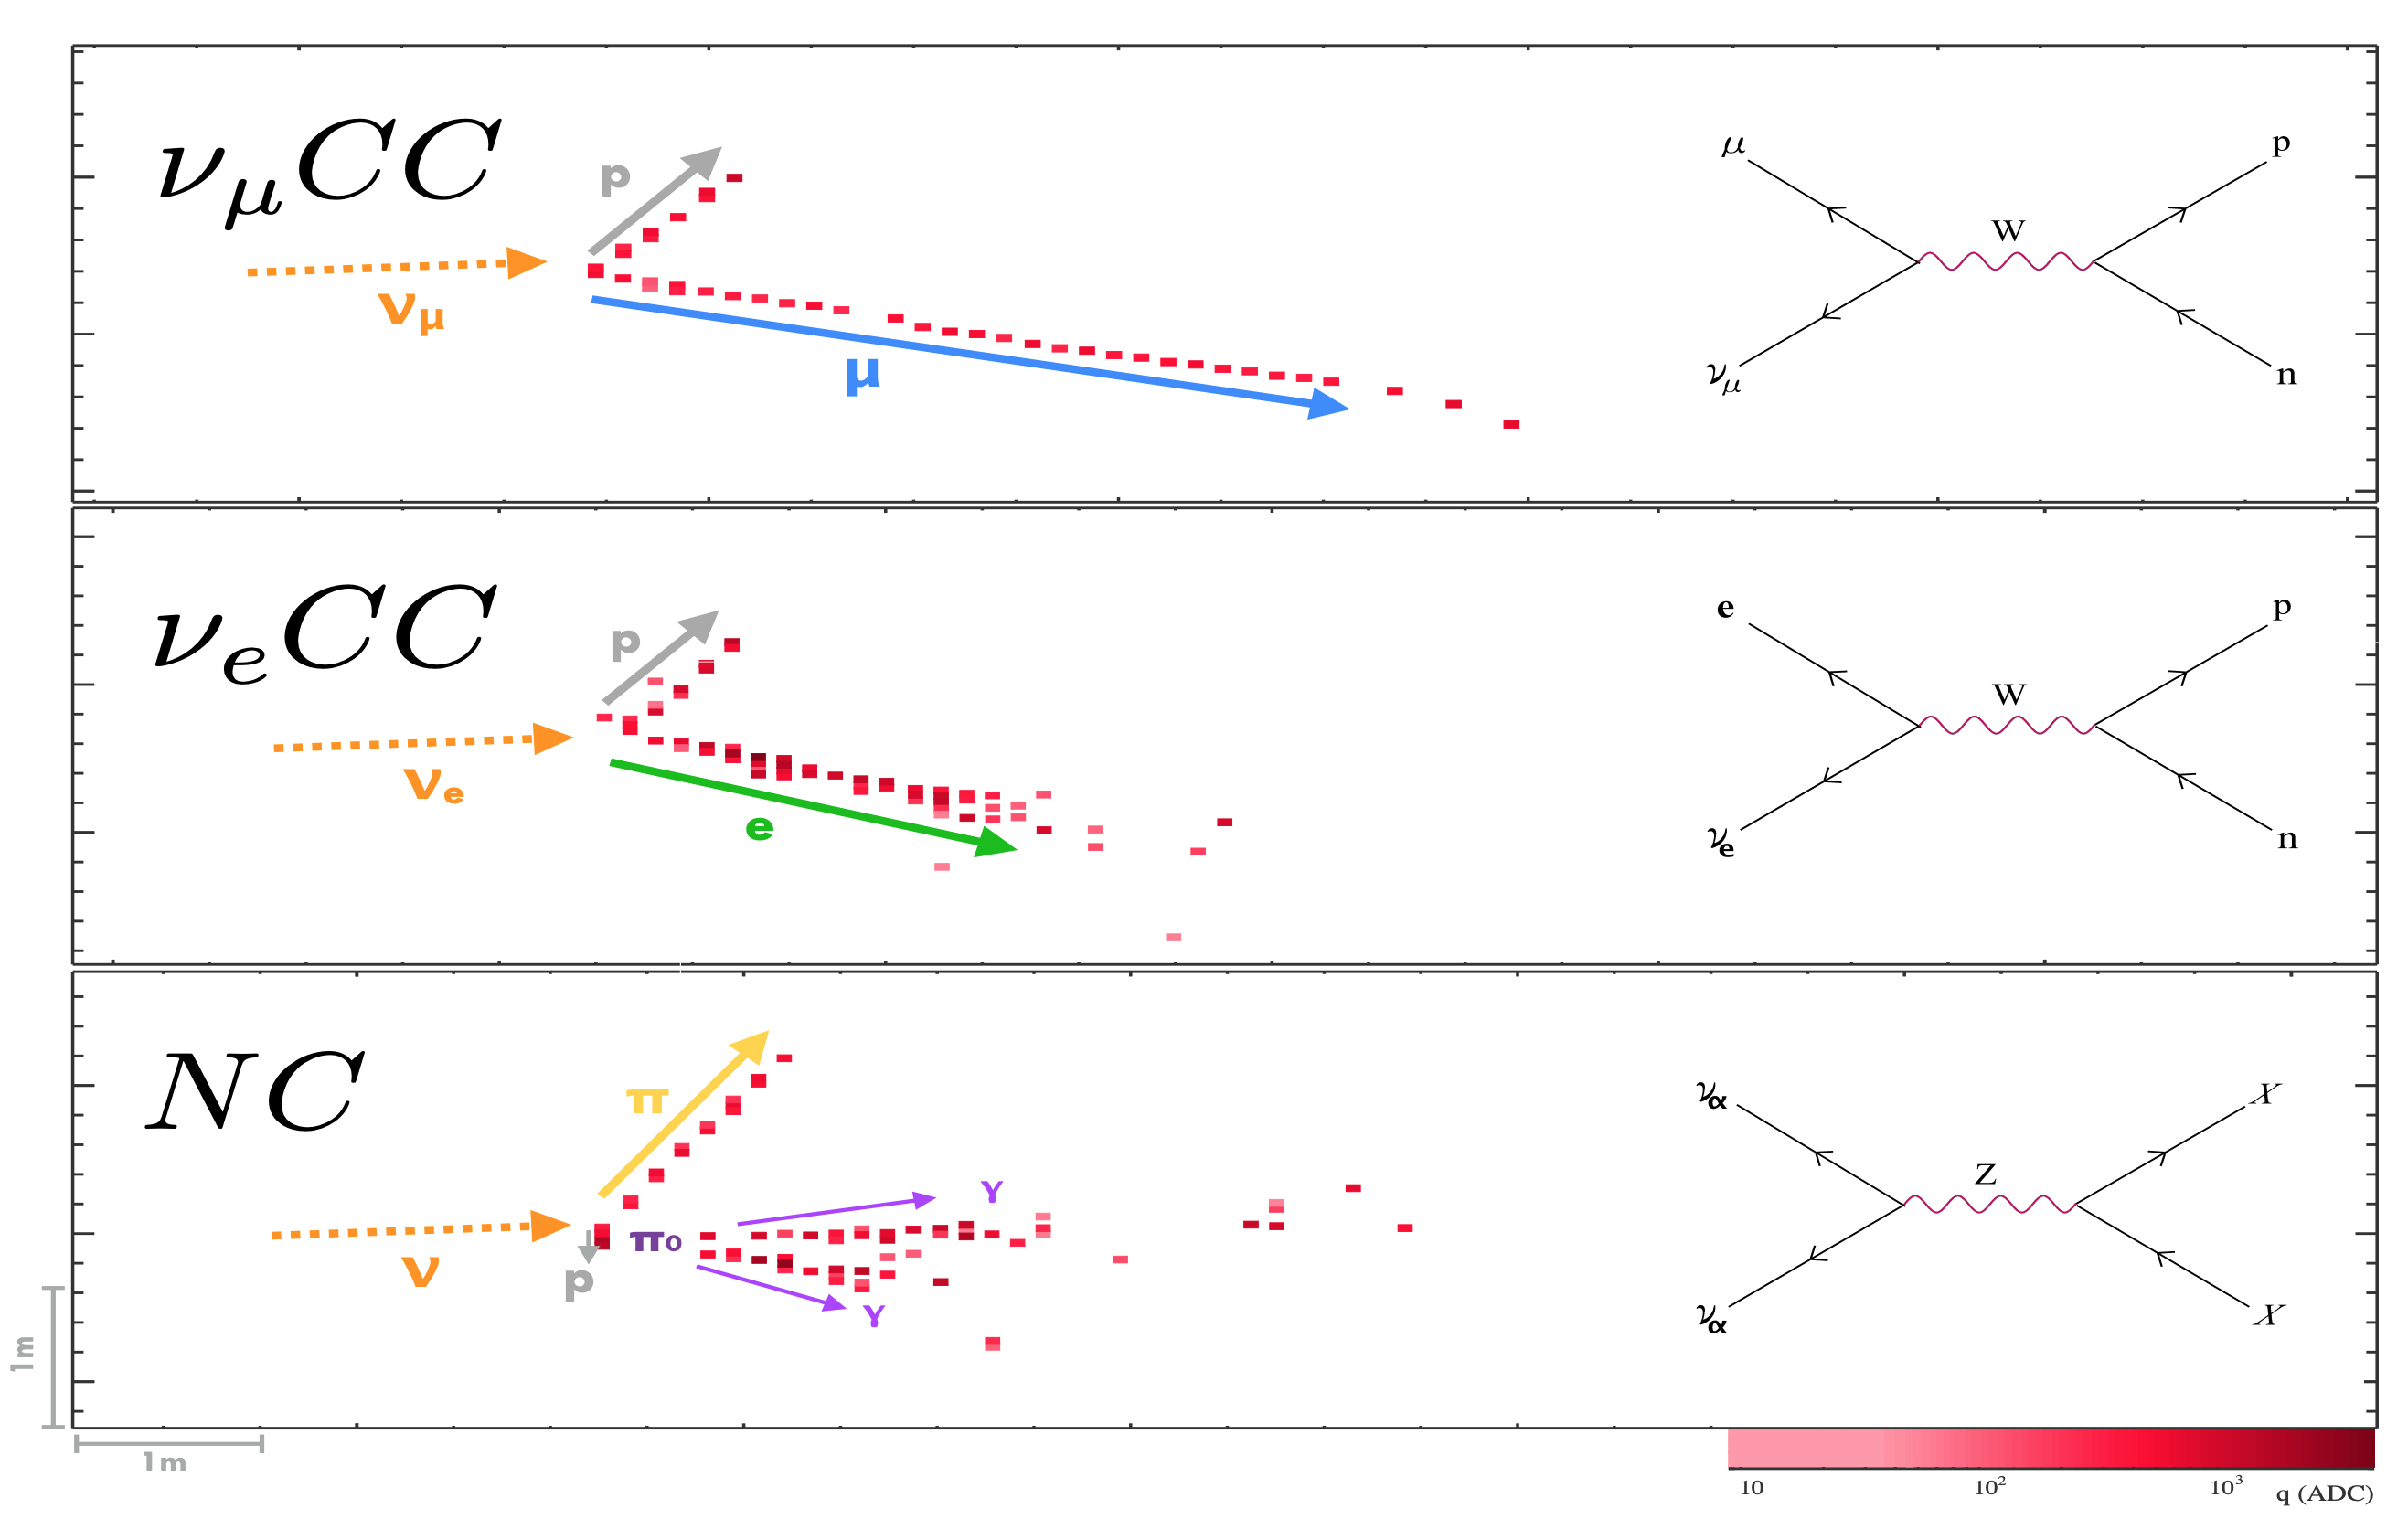
\includegraphics[scale=0.25]{Images/tracks.png}

 \textbf{Figure 1.} \textit{Three of the event topologies, for charged-current muon and electron neutrinos as well as a charged-neutral interaction, with their associated Feynman diagrams \cite{Singh}.}
\end{figure}

\noindent At NOvA a near detector, placed 1 km from the beam source, and a far detector, 810 km away, are used to determine the flavour of neutrino passing at each, and any changes to the neutrinos over the distance can be compared. By comparing the number of neutrinos of each flavour at the detectors, oscillation calculations can be made. \medskip

\noindent The detectors are a pair of finely grained liquid scintillator detectors. The near detector is 4m x 4m x 15m in size, with cells filled with liquid scintillator. Fibre optic cables collect the scintillation light to be stored. \medskip

\noindent The scintilator cells are arranged into planes, which are configured into horizontal and vertical alignments to provide separate, interleaved X-Z, and Y-Z views. The data therefore is displayed as the top view and side view of the detector, and these are what are used as inputs to the classification algorithm, see Figure 2 for a schematic of the detector and the output views.\medskip

\noindent A NuMI (Neutrinos at the Main Injector) beam, made of muon neutrinos is produced by firing protons into a graphine target, which produces pions amongst other particles. These pions are able to be directed by magnets in an intended direction of travel , before the pions decay into Muons and muon neutrinos. \cite{Ishitsuka} \medskip

\begin{figure}[t]
 \centering
 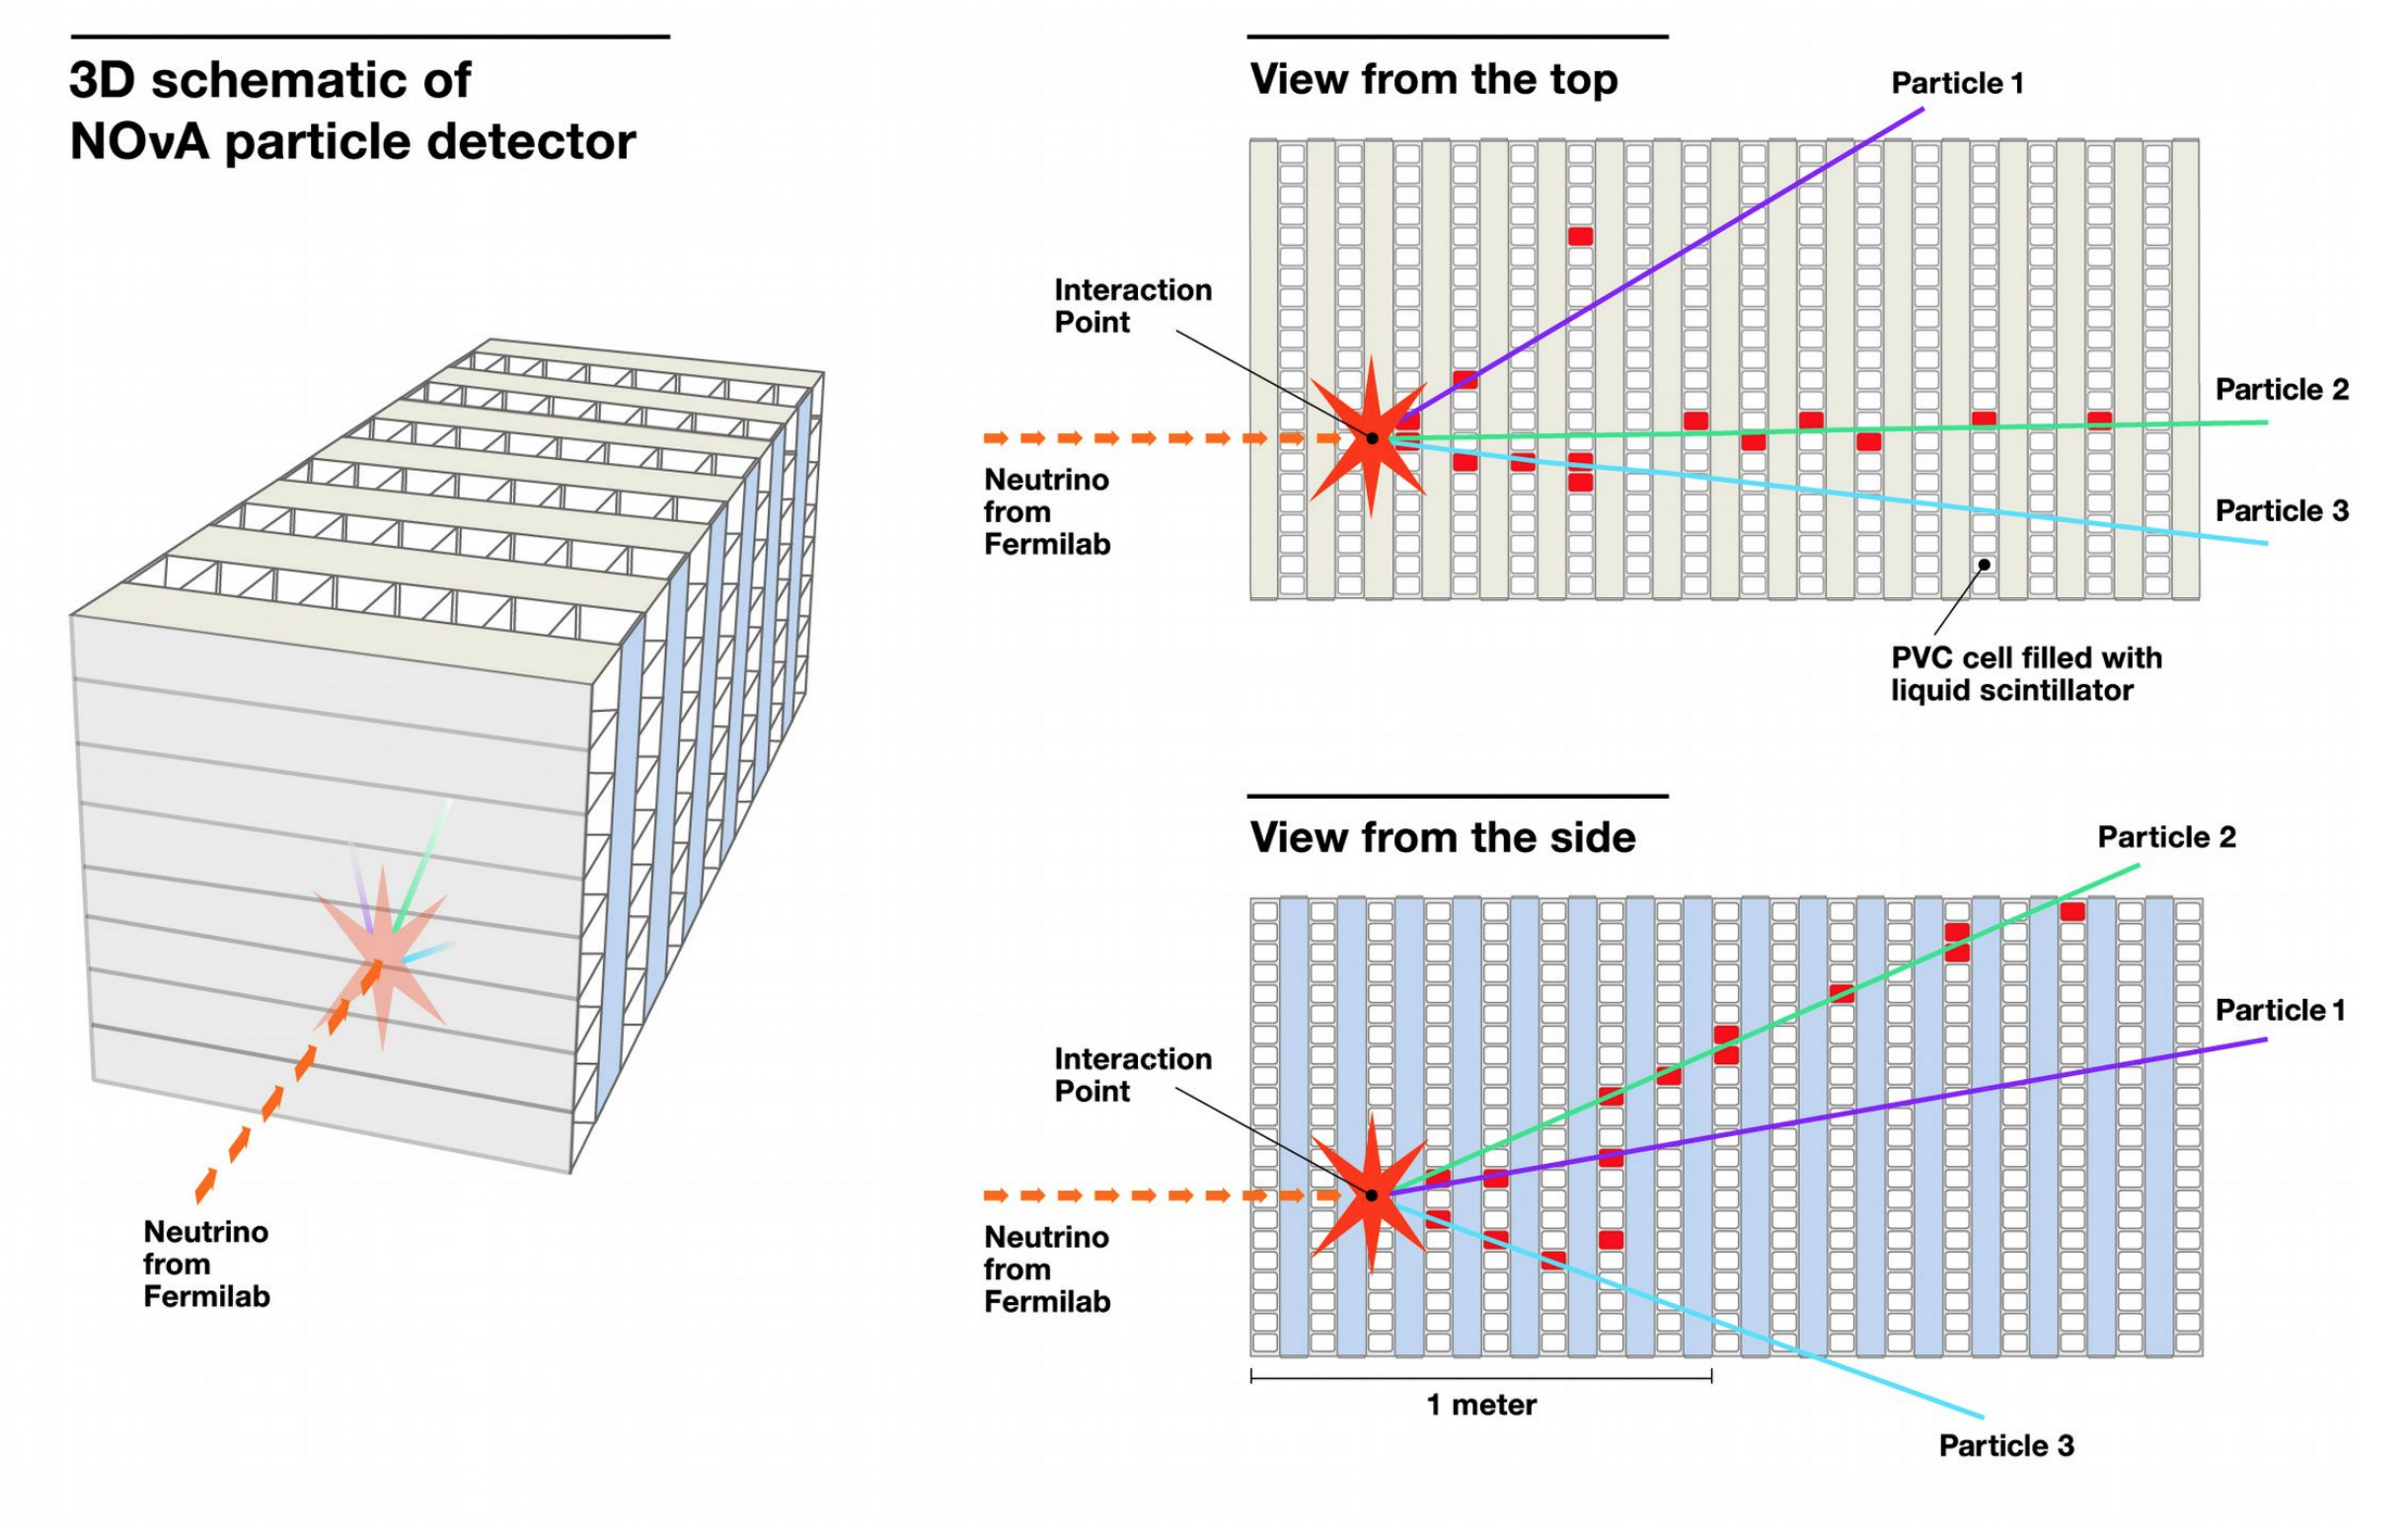
\includegraphics[scale=0.25]{Images/nova_nd.png} 
 
\textbf{ Figure 2.} \textit{Schematic of the NO$\nu$A scintilator detectors. The diagram on the left shows the 3D representation of the detector, while the diagrams on the right show the top view and side view planes where cell activation in each row or column indicate the tracks of the particles \cite{Aurisano}}.
\end{figure}

\noindent Traditionally classification required reconstructing high-level components associated with particle interactions such as clusters, tracks, showers, jets, and rings and summing the directions, and shapes of these objects, \cite{Aurisano}. However, the method now implemented at NOvA is a machine learning algorithm, where the model learns how to classify the interaction type from examples, a process known as supervised learning. Currently a CNN is being used, which has been found to be capable of pattern detection and particularly effective at image classification with real world photographs. \medskip

\noindent The network will look to classify the events based on features from the event topologies. $\nu_\mu$ events are indicated by a long, low dE/dx (energy loss per unit distance) track which is that of a minimally ionizing $\mu$, while $\nu_e$ events display a shower rather than a track . NC events can display both $\nu_\mu$ and  $\nu_e$ interaction like features- if the interaction produces pions. A charged pion track appears similar to that of a muon, except for an energy deposition spike at the end of the tracks; while the lifetime of a neutral pion is short, and it decays to produce electromagnetic shower, with the gap between the event vertex and shower the distinguishing factor from a $\nu_e$ event \cite{Aurisano}. \medskip

\noindent These similarities make the challenge of classification difficult, even for state of the art computer vision networks, however the performance compared to traditional reconstruction analysis showed positive results for these methods. NOvA's classifier, which at the time, was based on the GoogLeNet algorithm, that achieved an error rate of only 6.7\% on images \cite{Szegedy}, it now also uses the MobileNet algorthym that we will be using in this study, however they are yet to publish results of its performance. The network at NOvA outperforms the previous track-based modestly with a measurement-optimised efficiency of 58\% over the of 57\% from \cite{Adamson_1} for $\nu_\mu$ CC interactions and for $\nu_e$ CC interactions 49\% over the 35\% when compared to results from \cite{Adamson_2}. \medskip

\noindent In order to both learn how to classify as well as to validate the predictions against the actual classifications, the algorithms require labeled classification data as well as the event images. Data from the detector will not be labeled, thus simulated Monte Carlo event generators will provide the training examples; the two simulators that will be used are GENIE \cite{Andreopoulos_1} and GiBUU \cite{Lalakulich} however there are many different models that all simulate events uniquely. The GENIE Monte Carlo Simulation simulations the initial iteration of a neutrino with nuclei in the detector and the resulting scattered products to the surface of the nucleus \cite{Andreopoulos_2}. It mainly reproduces neutrino-nucleon scattering data but limited neutrino-nucleus scattering data means there are deficiencies in the primary physics model \cite{Perdue}. While the GiBUU simulation based on the Giessen–Boltzmann–Uehling– Uhlenbeck model which is a semiclassical transport model which describes the evolution of a many-body system in the presence of potentials and a collision term, with the addition  of neutrino-induced interactions. \medskip

\section{Machine Learning}

\noindent Artificial Neural networks (ANNs) \cite{McCulloch} are not a new phenomenon, however the recent increase in their popularity has come about due to the advances in hardware that allows the computationally expensive training of networks, which led to improvements in architectures and training processes. Neural networks increase in performance when given more data to learn from, and the volumes of data that are produced in this digital age has led to increased research into the development of theses algorithms. \medskip

\noindent In a traditional Feed Forward  Neural Network (FFNN), the most basic ANN, each neuron in each layer the output will be a weighted sum of the inputs from every neutron in the preceding layer, with this sum being passed to an activation function, which brings non-linearity allowing the modelling of more complex patterns \cite{Acciarri_2}. The output, $y_k$, for the $k^{th}$ neuron in a layer where $i = 1, 2,..., n$ where $n$ is the number of neutrons in the previous layer, and $x_{i}$ their corresponding outputs, with $w$, the weights, $b$, the bias, and $\sigma$ the activation function. \medskip

\[y_k = \sigma(\sum_{i}w_{ki} x_i +b)\]

\begin{figure}[t]
 \centering
 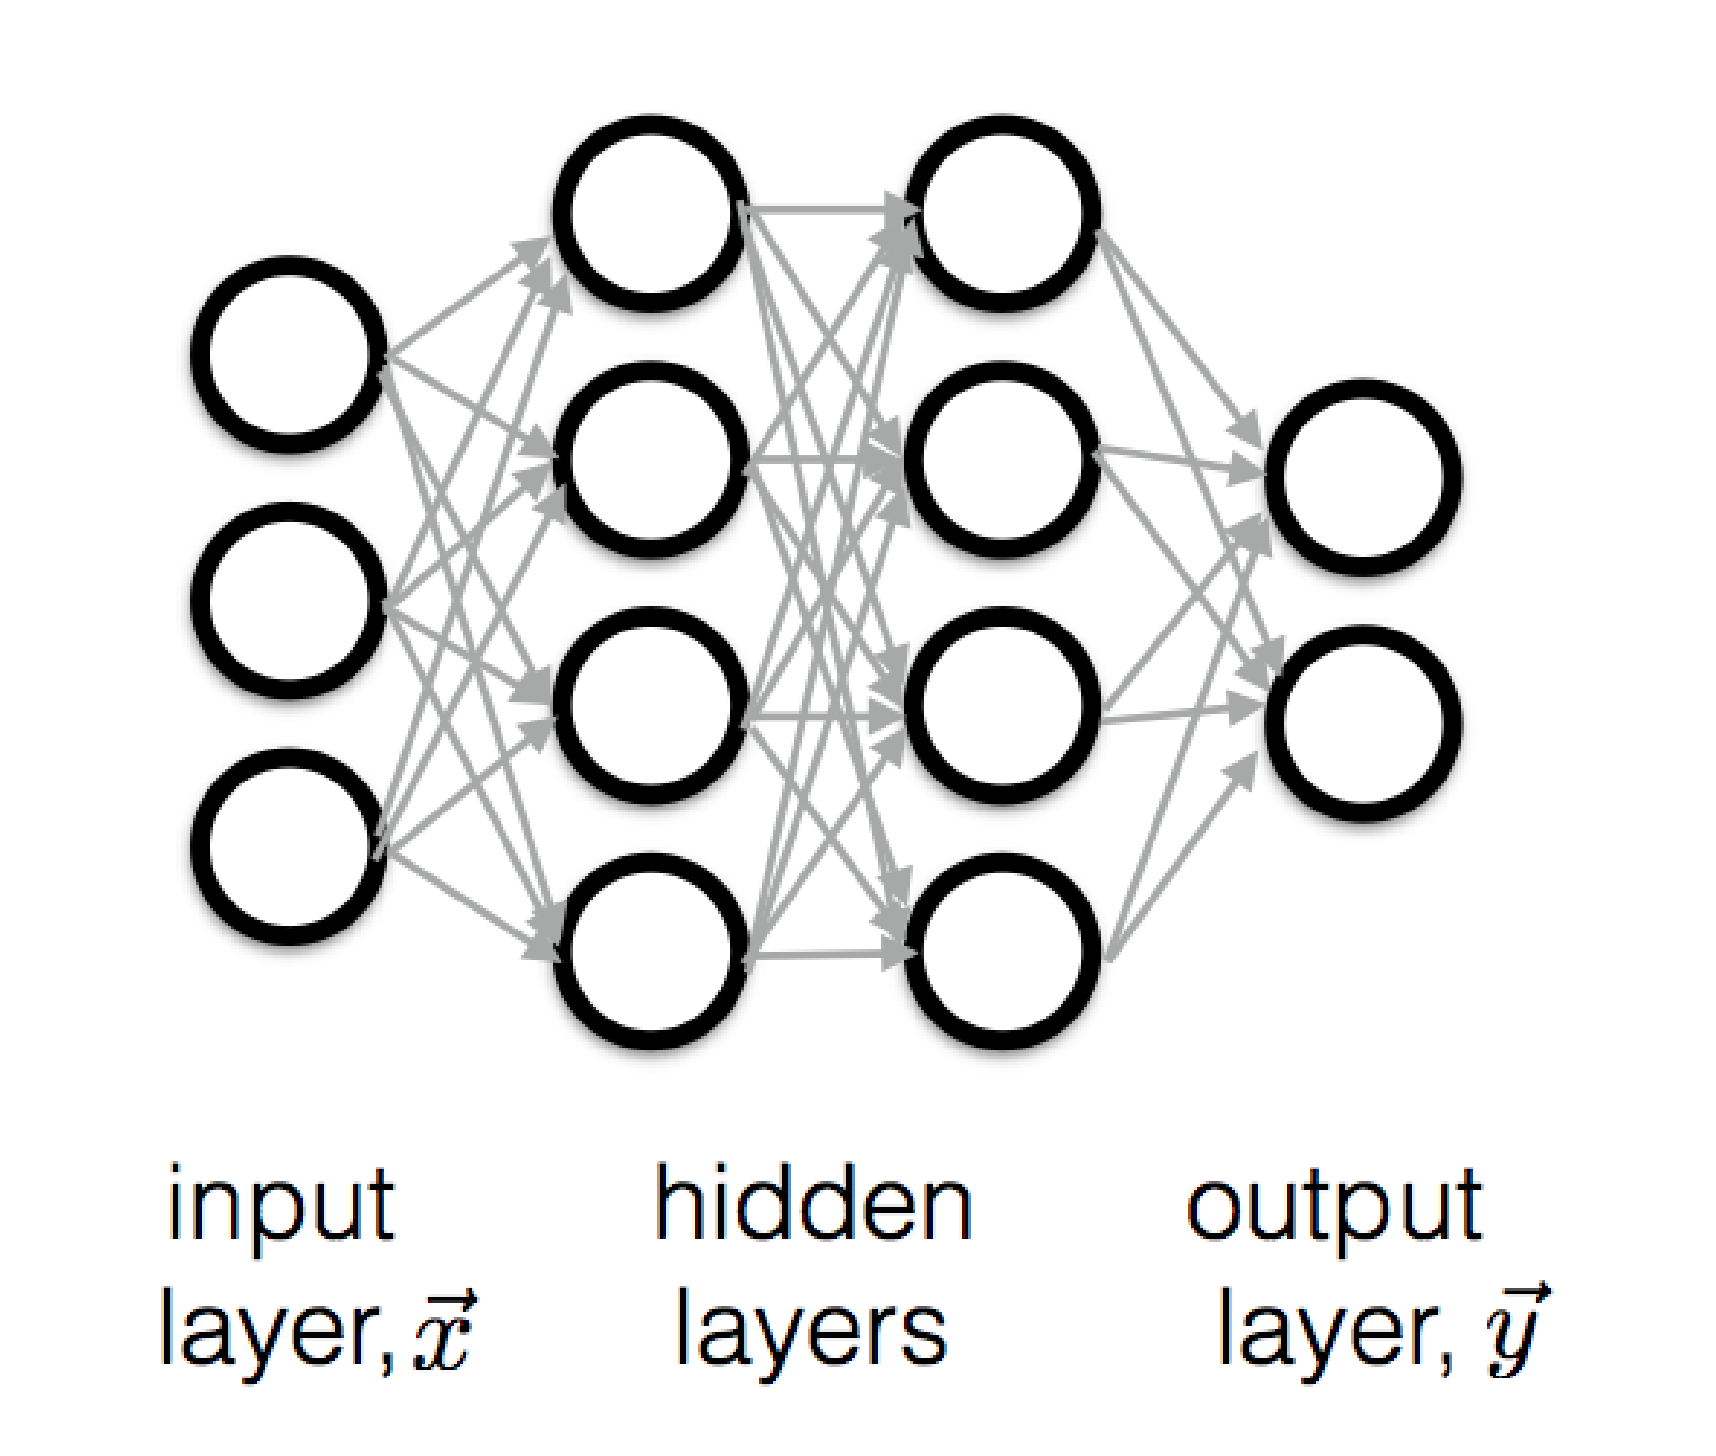
\includegraphics[scale=0.25]{Images/FFNN.png} 
 
 \textbf{Figure 3.} \textit{A graph of a simple FFNN with two hidden layers, that takes in 3 inputs that either classifies into one of two categories or produces two values depending on if the model is completing a classification or regression task. \cite{Acciarri_2}}
\end{figure}

\noindent The algorithm becomes connected network of these weighted sums, where the parameter weights, which are initially random, are learned by giving examples. The network will determine which patterns, or features, correspond to which event, and the algorithm tunes the weights values to produce the desired output through backpropagation. \medskip

\noindent The metric used to determine how effective the model is at the task is the loss function, which is measure of the error between the predicted output and the truth label. For a simple regression task this could be calculated using the mean absolute error or the mean squared error. In the case of particle identification, the problem is one of classification, and the loss function often takes the form of a cross-entropy function, which can be calculated by: 

\[L(y, \hat{y}) = - \sum_{i} y_{i} log(\hat{y}_{i})\]

\noindent where $y$ is the prediction, and $\hat{y}$ is the truth value, over the entire dataset. Here the functions compares the distribution of predictions to the one-hot-encoded true distribution, and the closer the the confidence of that class is to 1, the smaller the loss value. \medskip

\noindent The network looks to minimise the loss by updating the weights and biases of the network with each training step, a process that will fit the network to the data. In order to determine if the loss function is at a minimum, a method of gradient descent is used. The gradient of the loss function is calculated, and the is scaled by a learning rate. A large learning rate will mean that large steps are made, which will reduce the training time, but the optimisation may skip over the minima, while a small learning rate will take longer to converge, but will find the optimal value. Both these methods are subject to finding local minima, rather than the global minima, so stochastic optimiser algorithms are often used to allow for escaping minima, and over time should converge on the correct value. Optimisers often couple these gradient calculations with  variable learning rates, that start of large to allow the algorithm to search the surface, and then reduce in size to allow convergence to take place. \medskip

\noindent In order to prevent the network from continually converging on sub-optimal values, the initial weights are randomly determined. This means that each training process is unique, and the final model will be an ensemble of the models that are produced during each epoch- each pass over the training dataset. The neural networks have a large number of paramaters in order to be able to fit to complex input features, however the model may become too reliant on a small number of weights- which leads to overfitting to the training data, and struggling to generalise to new data. This is an area that will be discussed throughout this report. \medskip

\section{Convolutional Neural Networks}

\noindent In the field of computer vision, the most successful algorithms for pattern detection of images have proved to be Convolutional Neural Networks (CNN). These are ANNs that have been designed to space invariant, which makes them suited to processing images.

\noindent Much like a traditional FFNN, CNNs take in an input, have a number of hidden layers, and return an output; but work differently in that rather than every neuron being connected to each input value, a kernel, a small matrix, is passed over the image, pixel by pixel. This is due to the size of the input which can be several million pixels, where the process would become too computationally expensive to have fully connected layers. This kernel will apply a convolution function, using the pixel and the surrounding pixels as inputs to produce a weighted sum, see Figure 4, which it will produce another image from, with these convolutions detecting local structures \cite{Brenzke} such as edges or other patterns, building several feature maps and through training determining which combinations of these are most important to producing the correct output class, see Figure 5. Each layer passes multiple kernels over the same input, to produce a number of output matrices, all applying a different convolution, to form a tensor as the output.  (In this way, convolutional layers [29] produce many alternative representations of the input image, each serving to extract some feature which is learned from the training sample. \medskip

\begin{figure}[t]
 \centering
 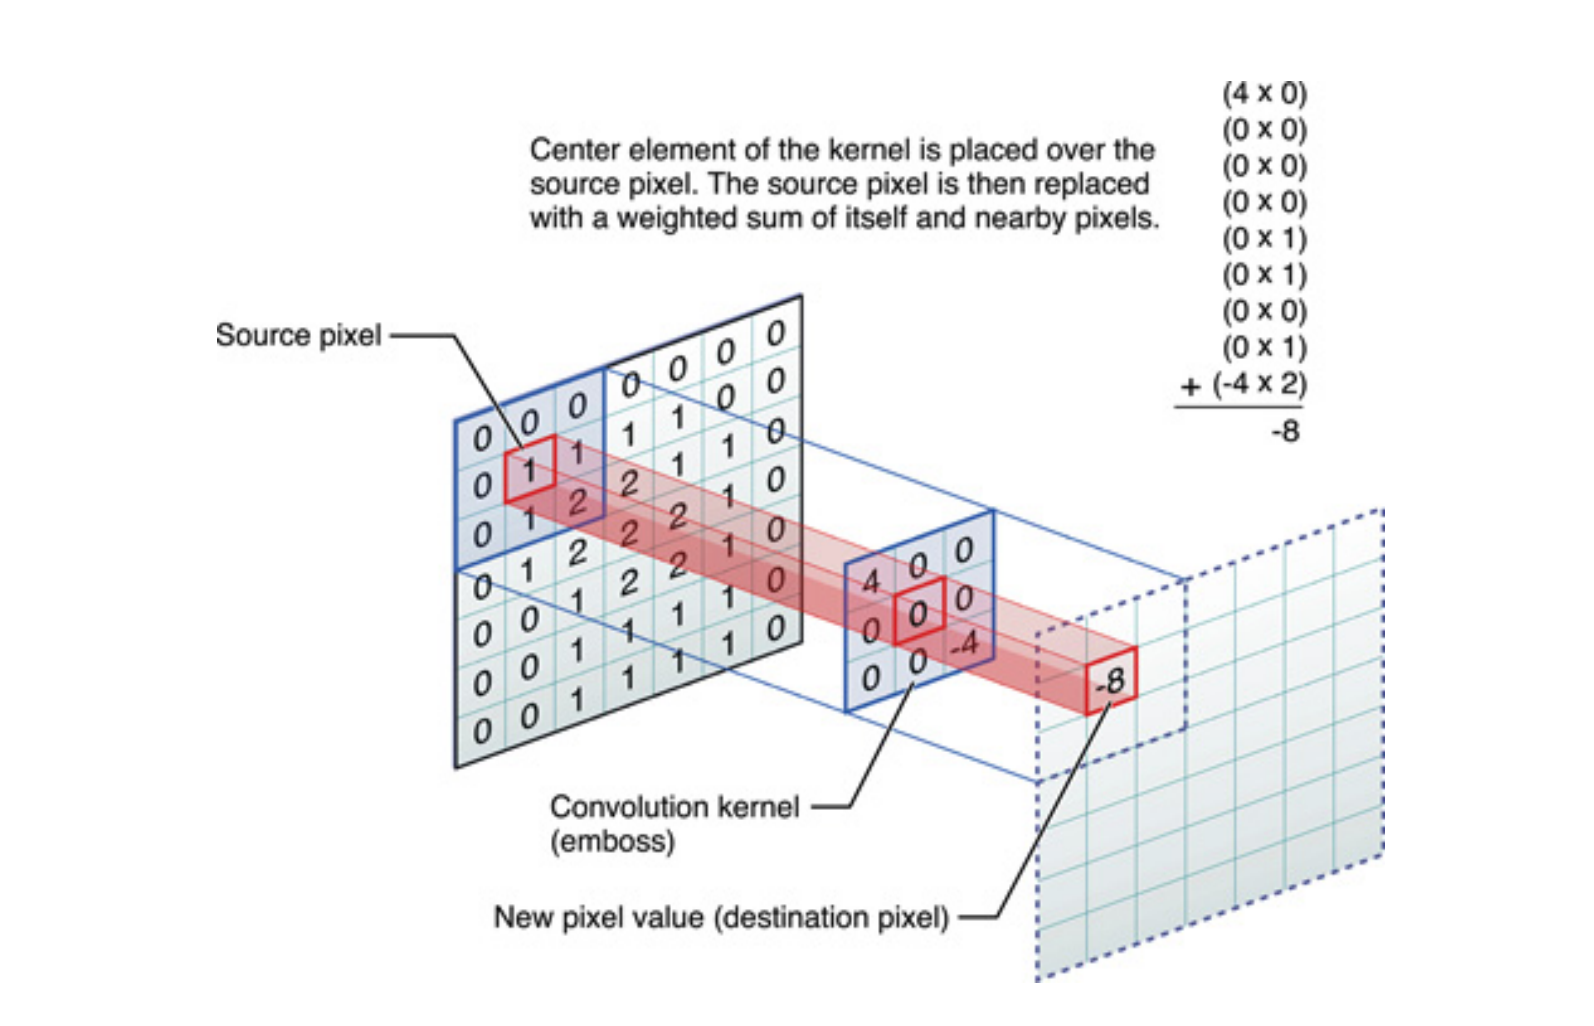
\includegraphics[scale=0.35]{Images/Conv.png} 
 
 \textbf{Figure 4.} \textit{Diagram of a Convolutional Kernel acting on a source matrix. The kernel is placed over a sub grid of the matrix, and the output value is determined by the product of the values in the input grid and the values in the kernel. The kernel then slides across the entire source matrix. \cite{Brenzke}.}
 \end{figure}
 
 \begin{figure}
 \centering
 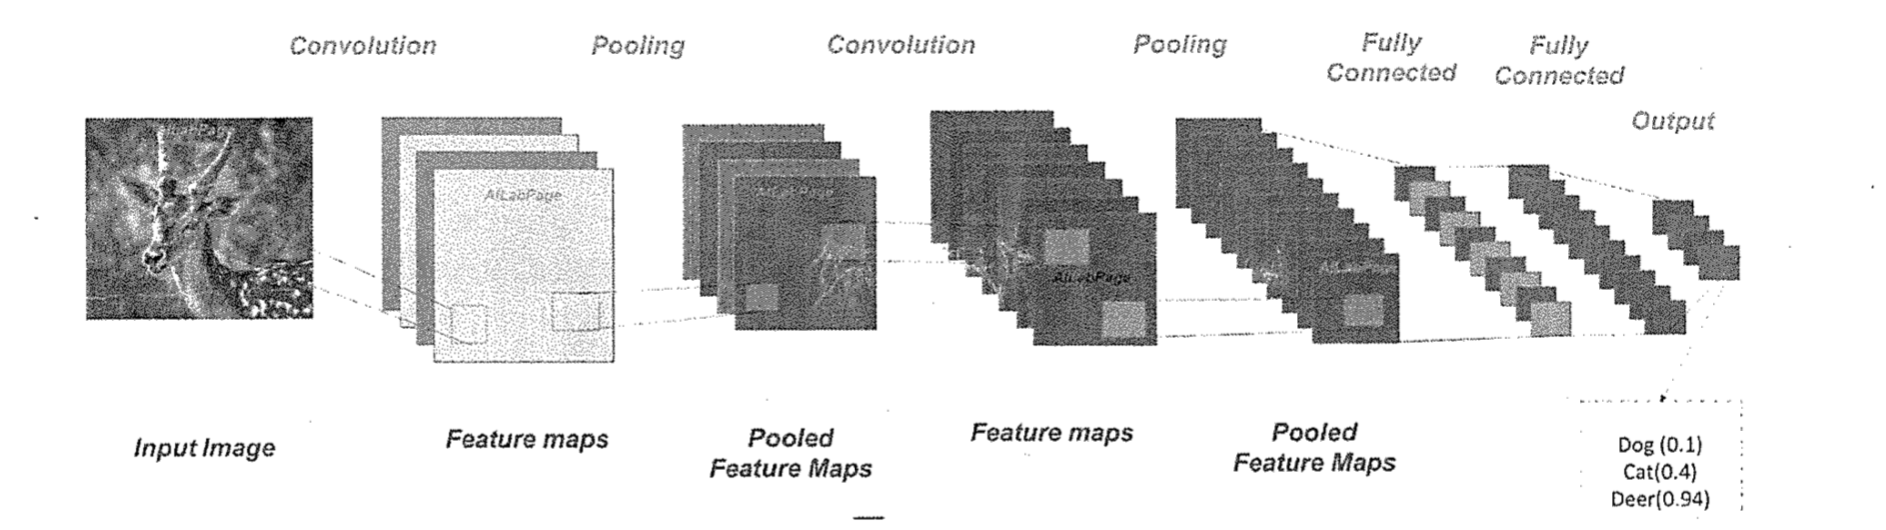
\includegraphics[scale=0.5]{Images/cnn_layers.png} 
 
  \textbf{Figure 5.} \textit{Architecture of a basic CNN, displaying the hidden convolution and pooling layers.}
 \end{figure}

\noindent In order for the network to be able to complete the process in a reasonable amount of time, each convolution layer is followed by a pooling layer, which reduces the size of output feature map by partitioning each matrix into subsections, where either the maximum value of the set (max pooling) or the average of the values (average pooling) is taken, reducing the number of parameters for each subsection to a single value. With these steps of convolutions and pools making up the majority of the layers in the network, producing a final vector, that feeds into a traditional FFNN to produce scores for the confidence level for each label it thinks it may be classifying. It is this output value that cuts are taken on when analysing data, using the simulation results where the score from the network is over a threshold value. \medskip

\section{Robustness}

\noindent A large problem that faces neural networks is the problem of overfitting. This is whereby the model becomes very good at picking up details from the dataset and essentially learns the dataset so much so that it struggles to then generalise on new data. In a CNN as there are fewer free parameters than with a fully connected network then the chance of overfitting is reduced \cite{Brenzke} and methods such as Dropout, which is zeroing random neurons in training so that that the network doesn’t rely on a small number of neurons, can help reduce this. Over a large number of training epochs, the  final network will be ensemble of smaller networks. However, they are still subject to becoming too specialised to the data they have been trained on, and the CNN being used to identify particle events, the model will be trained on the Monte Carlo simulations, neither of which perfectly model real events. This means that the model is susceptible to learning on these unrealistic data sets and becomes inaccurate when fitting for real data. \medskip

\noindent As the two simulations, GibUU differ on how they simulate different interactions, a part of the project was looking at how the models classify events from the two detectors. The robustness of the classifier will be determined by its ability to not show a domain-bias from the generators it was trained on, with the simulations based on models that are not identical to nature.\cite{Perdue} and that the model is able to generalise to incoming detector data. A classifier that is trained to pick up on small details in a dataset, that may be considered noise, will perform poorly on new data that is used in inference, especially if that data is from a different production source, such as a different generator or real detector data. By then poorly classifying incoming data, the experiment loses it's ability to make accurate measurements and identification of the neutrino flavours that are passing through the detector, and as a result loses the ability for accurate oscillation calculations to be made that look at the proportion of neutrinos that change flavour. \medskip

\noindent Many see machine learning algorithms, and in particular deep learning architectures, as black boxes because it is extremely difficult to interpret why they make the decisions they do. As discussed earlier,  the feed forward networks, after training, are a linear combination of the outputs from the nodes in the previous layer, passed through an activation function. Even by looking at the values of these weights and biases, one cannot understand how these values were chosen, and often they are not unique, as training an identical model with identical data will yield a different network, that may produce the same classification output, but have a different set of weights. This is due to the stochastic processes that underpin how the networks are trained, in both the initial weights values before training, and the stochastic processes that determine the loss function backpropagation gradients through the optimiser algorithms such as Adam or Stochastic Gradient Descent \cite{Kingma} . \medskip

\noindent When trying to interpret CNNs the feature maps range from high level features such as edges, to lower more abstract features that would be very difficult for a human to infer meaning from. Research is being undertaken to try and understand these black box algorithms such as \cite{Zhang} which looks at returning a filter over the input image that indicates which parts of the image were the strongest indicators to the network as to why the classification was made. \medskip

\noindent In the case of the particle physics events, the images represent the particle tracks and as a result do not contain as many features themselves as a picture of a object will making the training process for the network more difficult, and the features that the model uses to classify the image potentially more abstract. \medskip

\noindent This problem of interpretability posses a large problem with machine learning algorithms, not because of how they perform, but of whether they can be trusted to make decisions on the part of human experts, whether this being screening for cancers, determining how an autonomous car should act in a critical scenario, or determining whether to approve a mortgage. As a result, it is important that methods are developed to produce understand why these algorithms come to the decisions they do. \medskip

\section{Domain Adversarial Neural Networks}

\noindent An alternative network architecture that will be explored in this project is that of a DANN, which will be joined to the CNN classifier in order to reduce the domain dependence of the model \cite{Bousmalis}. Two sources of data, or domains, are introduced, a source domain where labels are available but not used so that the input is similar to unlabelled data from the target domain where labels are not available. The network produces two classified outputs, a features classifier, which predicts class labels in a way similar to a normal ANN, but also a domain classifier that discriminates between the source and target domains- determining which inputs are from simulations or detector data \cite{Ganin} or in the case of this project determining the inputs from the two different generators, as a proof of concept that in the future these techniques could improve the classification of detector data. \medskip

\noindent DANNs can also be applied to compare multiple simulation only datasets \cite{Perdue}, such as GENIE and GiBUU, to determine whether the network can tell which raw images belong to which. To have a robust model the network will need be invariant to the differences between these, as well as between the simulations and real data. Only data from the source domain is used to determine the parameters for the features classifier, with data from both domains determining those of the domain discriminator. By optimising for accuracy on the features classifier and maximising the error for the domain discriminator the classifier is trained to only use features in both domains. When an equilibrium is reached the domain discriminator is only able to distinguish samples from the sources by chance \cite{Louppe}. Figure 5 shows this additional part of the network, which in theory should produce a network trained to be invariant to the differences in the simulations as well as with real data, and results from \cite{Perdue} at MINERvA showed a small increase in accuracy at ~96\% to ~94.5\% for the domain trained networks.  \medskip

\begin{figure}[b!]
 \centering
 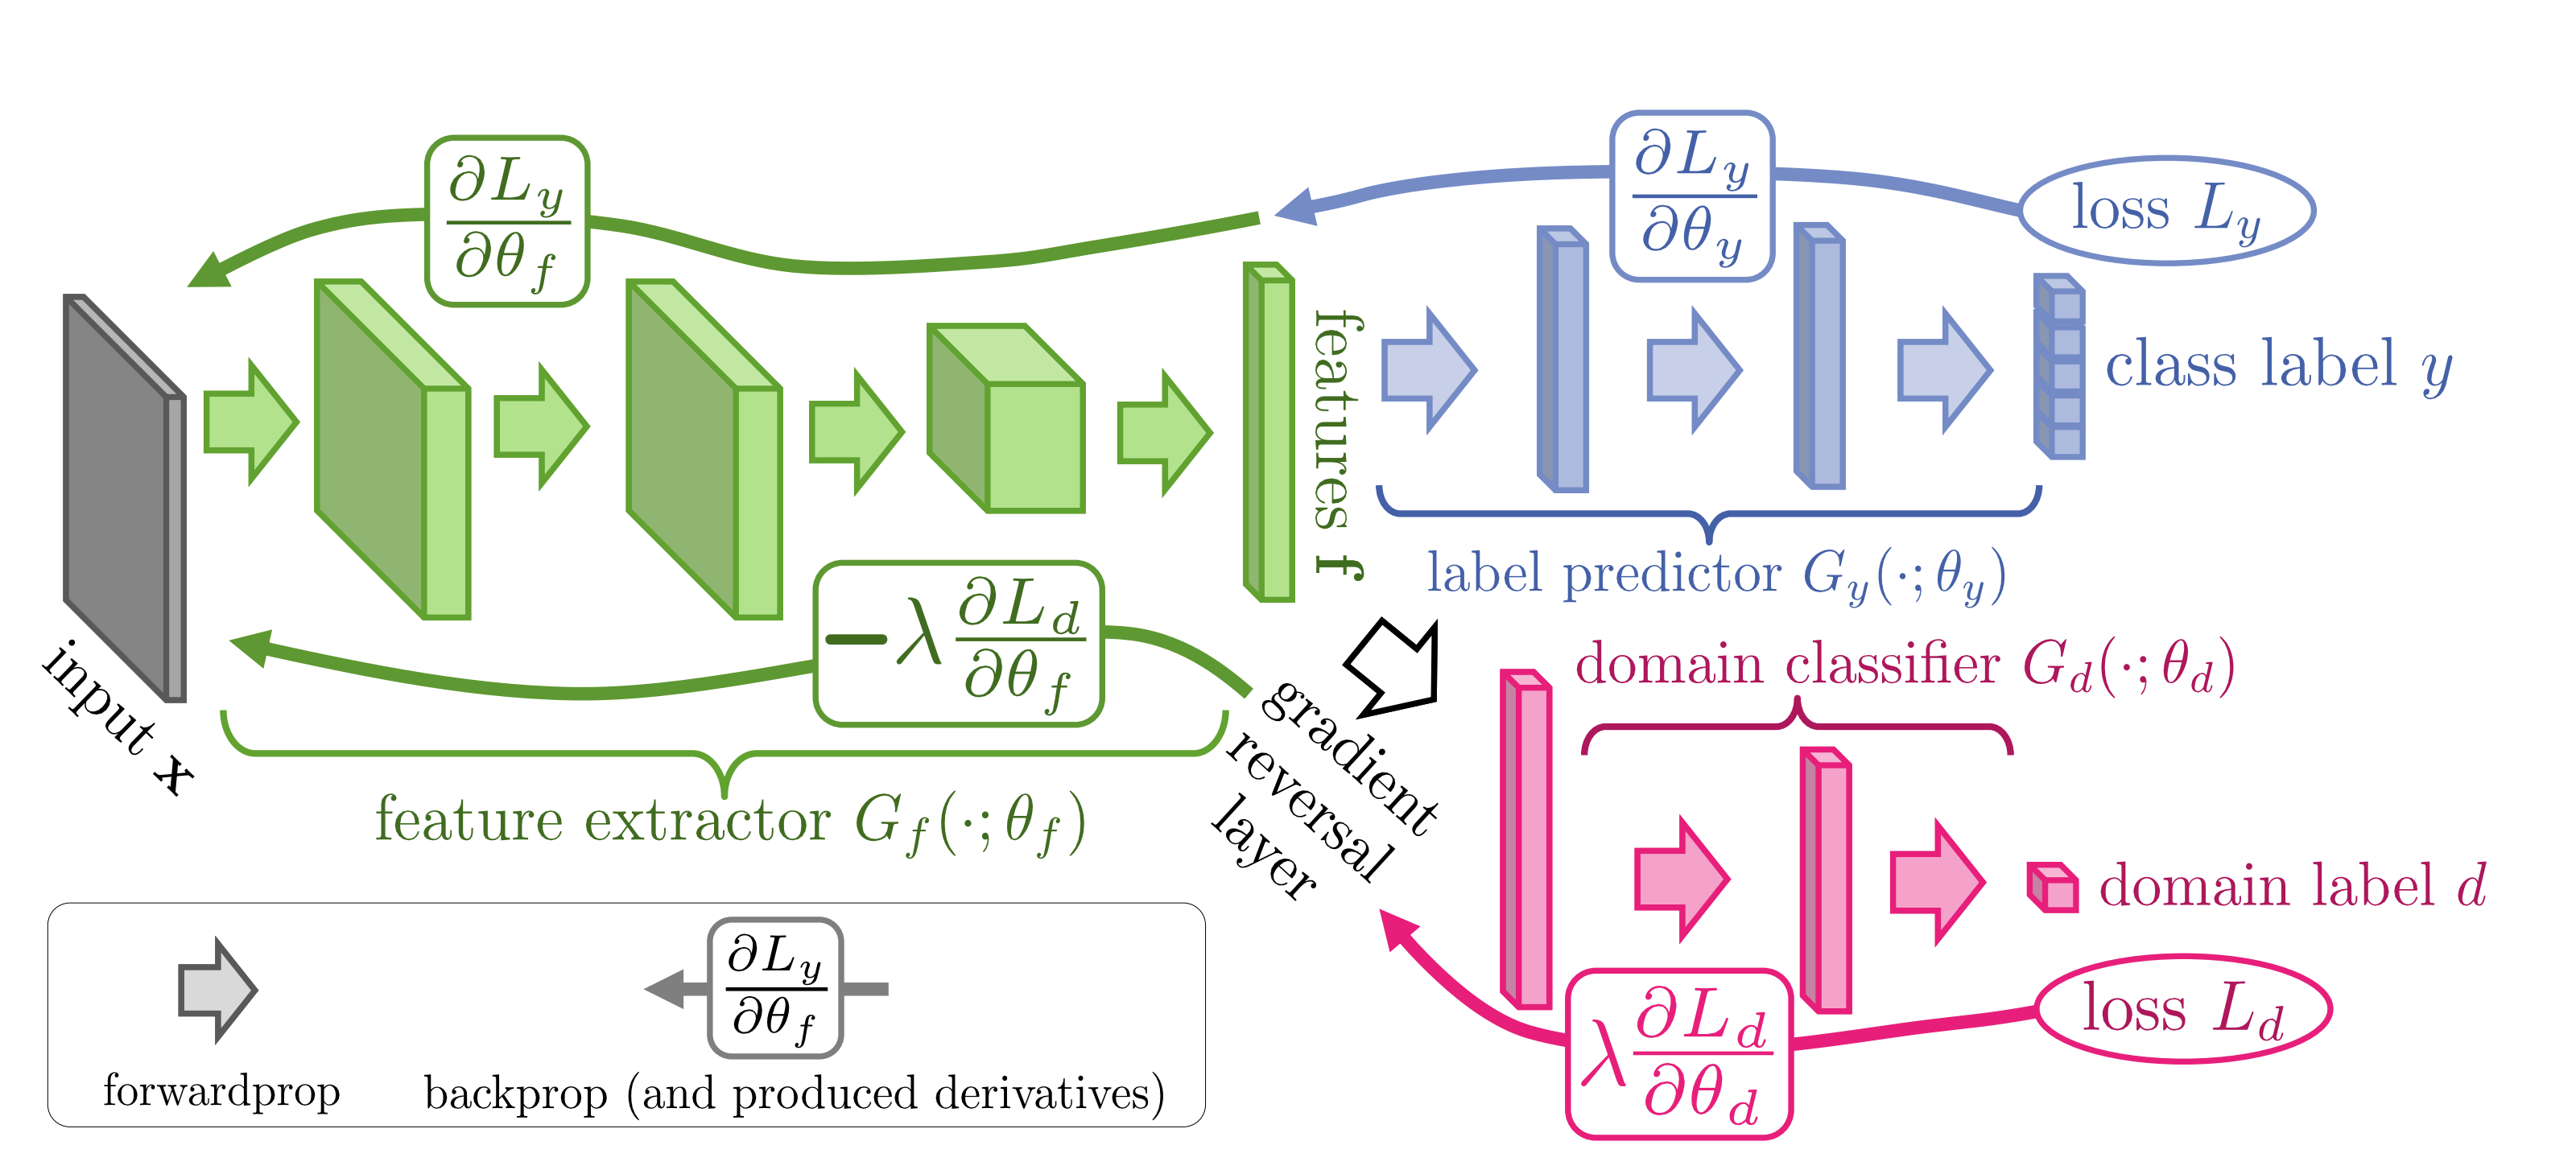
\includegraphics[scale=0.3]{Images/Dann.png} 
 
  \textbf{Figure 6.} \textit{Plot of the architecture of a DANN joined to a network, where $y$ is the outputs from the feature classifier and $d$ the  outputs of the domain classifier. The gradients show the error, or loss, functions that back-propogate to determine the weights and biases. \cite{Ganin}}
\end{figure}
\addtocontents{toc}{\vspace{-0.1cm}}
\chapter{Method}
\onehalfspacing

\section{Software}

\noindent The initial part of the project involved becoming familiar with the various technologies that are being used to analyse the data at NO$\nu$A. The data and software used to analyse the data are stored on the High Energy Physics group’s Linux cluster of machines, running both Scientific Linux, meaning that it was essential understand the Linux command line in order to navigate the file system and software packages, as well as run and debug scripts. \medskip

\noindent NO$\nu$ASoft is a software package, developed by Fermilab, that builds on the ROOT data analysis software \cite{Brun}, developed by CERN. CAFAna is the framework that NO$\nu$ASoft uses to run functions and produce plots by specifying cuts on the data. The  analysis framework is written in C++, a language I had no prior experience of, so a proportion of the time was spent trying to interpret pre-existing C++ scripts in NO$\nu$ASoft, as well as the doxygen documentation. \medskip



\section{Training data}

\noindent The MC data is stored as ROOT files, as well as HDF5 files that contain the training data. The image data comes in the form of an array and the interaction targets in the form of a ‘pdg’ (particle data group) value. The event labels are stored as part of ‘mc’ branch of the HDF5 file, while the input images are stored in a ‘training’ branch. \medskip

\noindent The data stored in these HDF5 files has already undergone preselection cuts- this was indicated by the fact that the number of subevents stored in the ‘mc’ branch is larger than that of the ‘training’ branch. Because of this, the events could not simply be matched up based on their index value, but on the following values: ‘run’, ‘subrun’, ‘evt’ (event), ‘subevt’ (sub event) and ‘cycle’ to indicate which subevent is being referenced. \medskip

\noindent After reshaping the image maps from a 1D array to two 100 x 80 pixel images representing the z-x and z-y planes of the detector (see Figure 7 for plots of an event in the two detector planes), the images were written to a 4D tensor with dimensions:
{\begin{itemize}
 \vspace*{-3mm}
\item event index (determined by the order that the images were added),
 \vspace*{-3mm}
\item plane (z-x or z-y),
 \vspace*{-3mm}
\item z value,
 \vspace*{-3mm}
\item x or y value.
 \vspace*{-3mm}
  \end{itemize}}
    
\begin{figure}[t!]
 \centering
 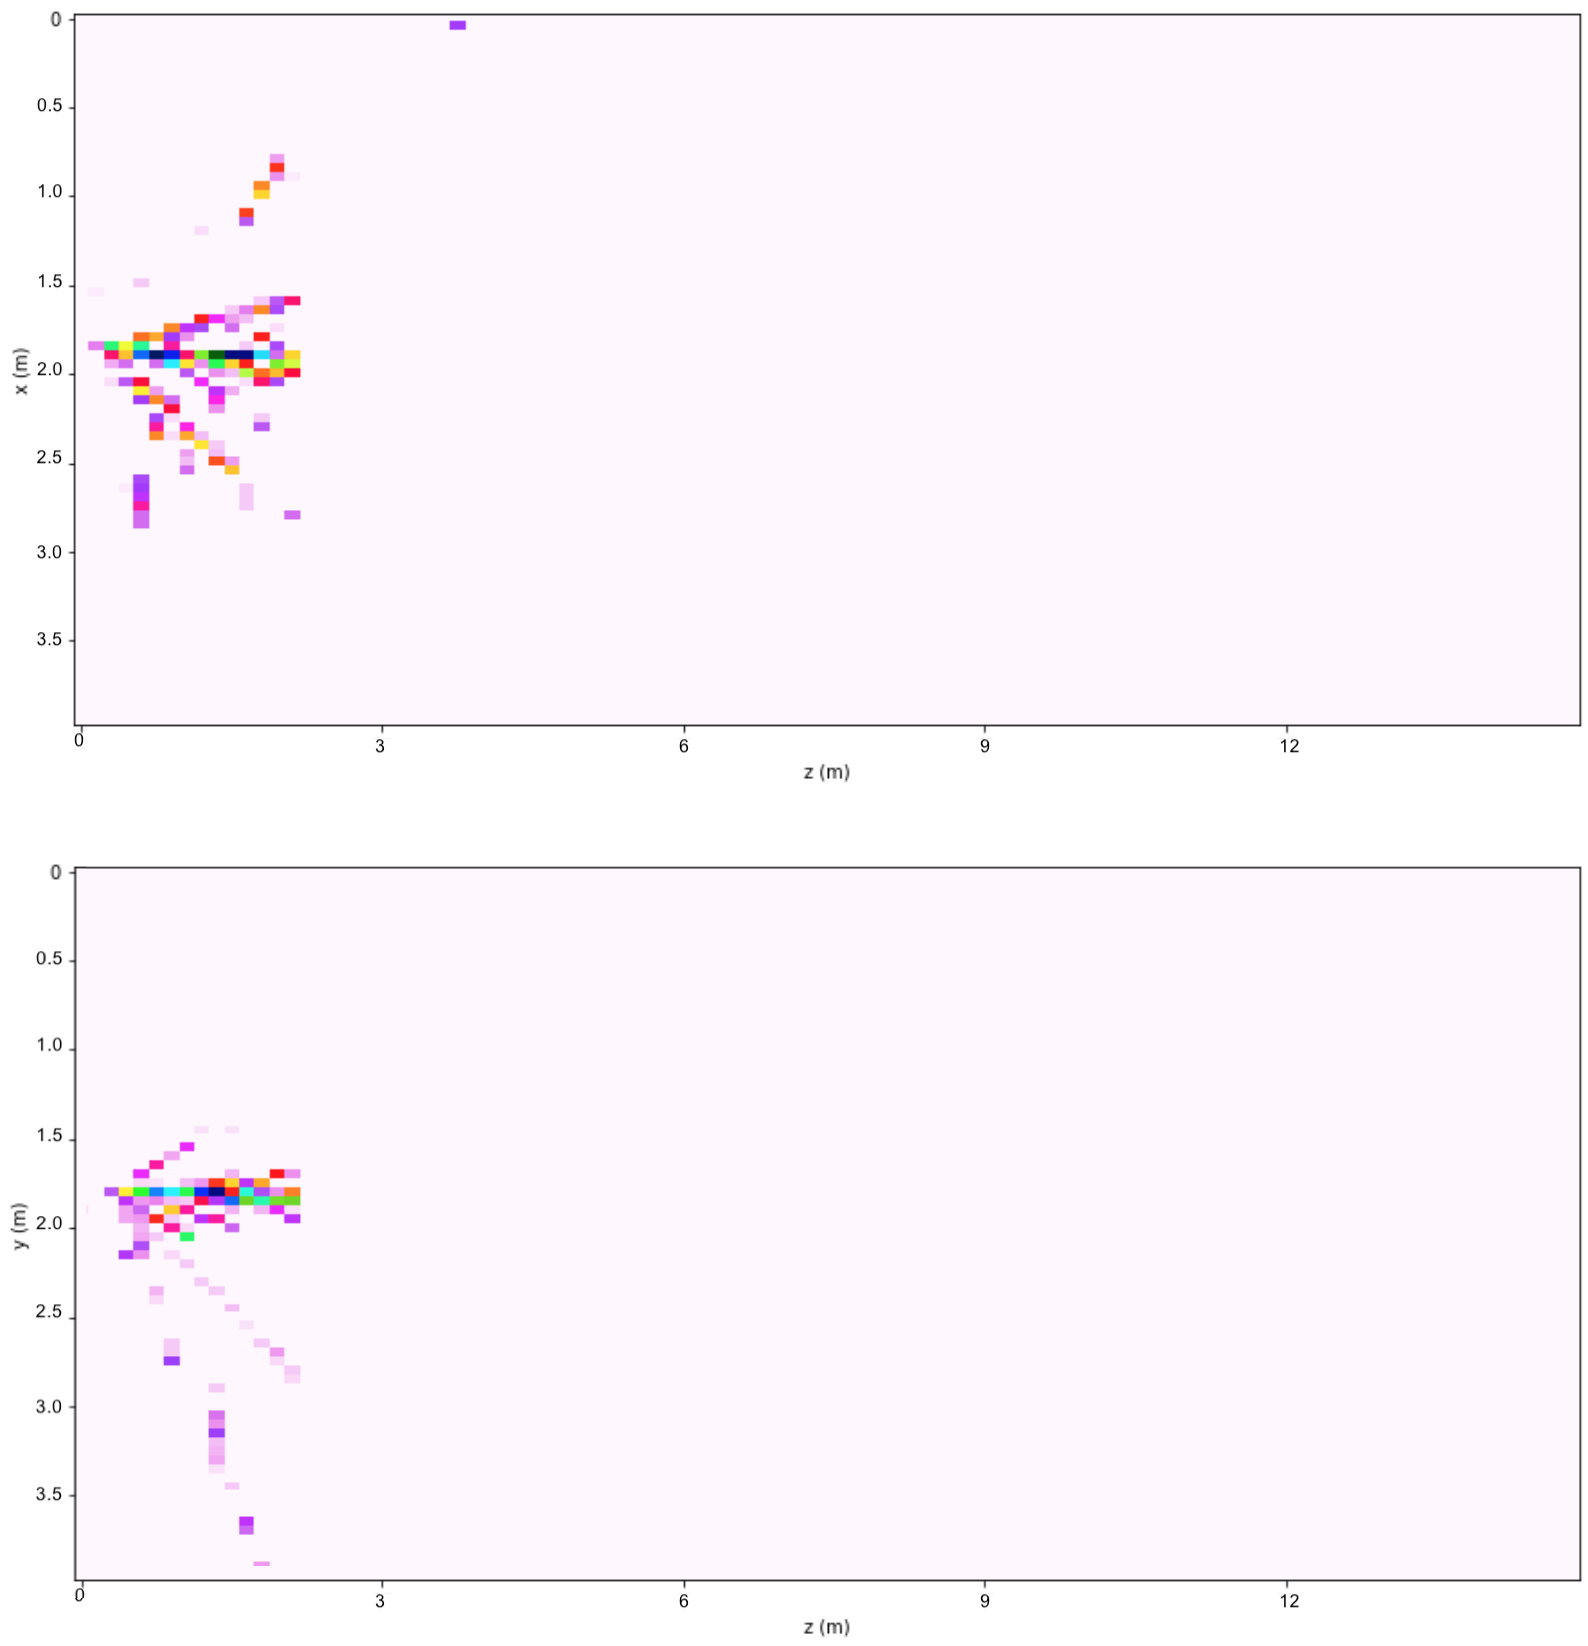
\includegraphics[width=120mm]{Images/xyzplots.png}
 
 \textbf{Figure 7.} \textit{Plot showing an event from the two planes of the detector (z-x and z-y) .}
\end{figure}

\noindent The HDF5 files also store data about each event, and this was used to apply the basic quality and preselection cuts. The cuts were outlined in the NO$\nu$A doxygen with the $\nu_\mu$ cuts as to remove any events that could be considered background events. These could be, for example atmospheric neutrinos, as well as neutrinos produced on earth, or from another process, and would be removed by the Cosmic Rejection cuts and the preselection cuts, as well as basic quality cuts.\medskip

\noindent Much like the the code already for the NO$\nu$A project and NO$\nu$Asoft, these are written in C++ and use the branch like structure of the ROOT files. A package has been developed for Python, called Pandana, however, I am unfamiliar with the syntax associated with the package and the documentation seems to focus on network analysis, so I deemed it a simpler option to simply implement the cuts using if statements with a loop over all the events. \medskip

\noindent While this meant that the computational process is much slower, I didn't see that as a problem as the cuts need only be applied once, for each generator, and the events that pass can be stored and then used as model inputs from then onward. In order to verify that the cuts that I had made were correct, a function had been written in NO$\nu$ASoft, ‘MakeEventListFile’, that listed the events that pass a specific cut, in order to be able to cross reference with the results I obtained.\medskip

\noindent It may be useful to learn and then implement the Pandana approach if more training data needs to be used in the future, or if the network was to be trained dynamically in the future.\medskip

\noindent While Keras does have a C++ API, as well as the option to export a model from Python, as Python is the language I am more comfortable with I decided that it was worthwhile interpreting the cuts and implementing them in Python rather than using the pre-existing C++ functions.\medskip

\section{Models}

\noindent The data that passed the preselection cuts, now in the form of image maps and labels indicating the interaction type, were now able to be passed to a model for training. Initially this was done on a smaller scale, using just 10 of the available 1150 files in order to ensure that all components were working properly. The interaction labels are one hot encoded into three classes: neutral current (NC), charged current  (CC) $\nu_e$  (and  ${\overline{\nu}_e}$) , CC $\nu_\mu$  (and  ${\overline{\nu}_\mu}$) as the classifier makes predictions for if an event belongs to each class.\medskip

\noindent Initially I produced a small network containing 6 sequential blocks containing convolution, max pooling and drop out layers in Keras. I did this to understand whether there were any errors in the formatting of the data as I was familiar with what was required for my rudimentary model. This worked with no hiccups, although the classifier was not particularly accurate. \medskip

\noindent The next stage was to run the small dataset using the MobileNet \cite{Sandler} architecture, developed by Google.  MobileNet is designed for implementation on mobile devices with a reduced computing power and thus reduced the training time significantly. As the computational facilities at the HEP Linux cluster I was using for the project do not have GPU cores to train the models, this more memory and processor efficient network made training more efficient that even my simple sequential network, despite being a more complex and having a much larger number of trainable parameters.\medskip

\noindent Literature stated that MobileNet does experience a reduction in classification performance \cite{Brun}, however the increase in performance time is significant and more valuable to a project with a limited timeframe, which is looking to see if new methods can be implemented, as opposed to producing a final production model.\medskip

\noindent The MobileNet architecture, officially known as MobileNetV2, uses 'depthwise separable convolutions', 'linear bottlenecks' and 'inverted residuals' to improve the training time and memory efficiency. \cite{Sandler}. MobileNet applies 3 x 3 depthwise separable convolutions that replace conventional convolutions, by first applying a single convolutional filter before a 1x1 convolution builds new feature maps through linear combinations of the inputs. Linear bottlenecks project, or embed, the feature maps to a lower-dimensional spaces, and it is this projection that leads to the loss in information, but reduced training time. Rather than use a non-linear activation function such as ReLU, a linear one is used instead to prevent a loss of information during the transform. The inverted residuals act as feature map expansions from the low-dimensional space.\medskip

\noindent In this project the MobileNet architecture was altered to take in two images per event, for the two planes of the detector, and process these in parallel before concatenated them together before rest of the network processed the inputs.\medskip

\noindent The network produces probabilities for each category indicating the confidence level that the network has in belonging to each label class. By taking the category that the model is most confident of we can compare this to the MC truth data we obtain the accuracy values, and the loss values that the loss values that the training process uses to indicate the success of the training. \medskip

\section{Generator Method}

\noindent While it was possible to write the required data to an array when working with a relatively small dataset, this was not possible when using all of the available files in the directory- 1150 GENIE HDF5 files, each with approximately 8370 events, totalling 9625500 events in total.
As a result I decided to produce a data frame for the events that passed the cuts, storing the following data about the event, but not the image map itself. The columns of the dataframe were as follows:
{\begin{itemize}
 \vspace*{-3mm}
\item ‘run’ ,
 \vspace*{-3mm}
\item ‘subrun’,
 \vspace*{-3mm}
\item ‘evt’ (event),
 \vspace*{-3mm}
\item ‘subevt’ (sub event),
 \vspace*{-3mm}
 \item ‘cycle’,
 \vspace*{-3mm}
\item ‘train\_index’:  location index within the ‘training branch’ of the image,
 \vspace*{-3mm}
\item ‘label’ : pdg interaction value,
 \vspace*{-3mm}
\item ‘file’: path to the relevant HDF5 file. 
  \end{itemize}}

\noindent The data frames were then concatenated to produce three: one for training containing 335,456 sub events, one for training validation containing 67,092 sub events, and one for testing the model containing 93,248 sub events.\medskip

\noindent As the data was not stored locally, the data could not be loaded into the model all at once. Keras allows for a generator to load the data to the model in various batch sizes. This sources the image data from the relevant HDF5 file using the location stored in the ‘file’ column of the data frame and the 'train\_index' value from that row to identify the array in question. This is then reshaped the same way as before and written to a 4D tensor identical to the one for the entire dataset, with the only difference being the event index dimension is the size of the batch size that is specified, rather than the entire dataset. The default batch size is 32, as is the case with the results produced by NO$\nu$A\cite{Aurisano}. The target values are again one-hot encoded based on the ‘label’ value for the row.\medskip

\noindent The GiBUU events are similar to the genie events in the way that the data is stored in the HDF5 files, so an identical approach could be used to preselect data and store the corresponding data regarding the events in a dataframe, that also contained the location of the training images, as was with the GENIE events. The GiBUU events have an additional property, being that each event is given a weight value. These weight values were contained in the HDF5 files, however they were incorrect- with values ranging from the order of 10\textsuperscript{-3} to 10\textsuperscript{4}. A NO$\nu$ASoft function had been written to correct this, but as I was not using the ROOT files, but the HDF5 files I could not directly apply the function to the values in the HDF5 files. As well as this the function relied on a large number of C++ dependency files that made it an unreasonable task to try and replicate the function in Python, as had been done with the preselection cuts.\medskip

\noindent Once again the ‘MakeEventListFile' function could be used to create a text file with the associated weight value for each event. Then a mapping function could be used to add the weight value to the correspoding event.\medskip

\noindent In the training process the weight was used to provide a the weighing that each particular event should have on the overall statistics of the dataset. In our case that indicated the importance of the event to the training process. I was unable to find a method in Keras that allowed for a weighted training procedure, that being one where the magnitudes of the gradients calculated for the gradient descent backpropagation process were scaled in accordance with the GiBUU weights. This gradient scaling was used when training the DANN as will be discussed later, however every event was scaled by a constant value in that case, rather than changing for every event here. The tensor batch preprossessing in the MobileNet architecture applies a 'Subnet' process to the batch that meant that I could not ensure that the associated weight would correspond correctly when calculating the gradients for each event without extensive testing that I did not think could be completed within the timeframe of the project.\medskip

\noindent Alternatively, the weight was used as a value that indicated the likelihood that the event would be included in the training procedure. A random number was generated between 1 and 10, which was the range in which almost all of the weights values were contained, with the exception of a few that were greater in value. If the weight value of an event that had passed the preselection cuts was greater than the random generated value the event data was written to the dataframe. If it was lower it was passed and the next event was evaluated in the same way.As the GENIE events did not contain this weight value, all the GENIE events that passed the preselection cuts were written to the train, validate and test dataframes.\medskip

\noindent This process did mean that a large proportion of the GiBUU events were not used in the training process, however this was not as large of a problem, as the number of GiBUU events given far exceeded the number of GENIE events available, and as will be discussed in the imbalanced dataset section, as we as the computational expense section, I would not have been reasonable to train the model using all of these events anyway.\medskip

\noindent Once these dataframes had been produced, a generator function could load in the data to the models for training.

\section{Hyperarameters}

\noindent A neural network is defined by a number of hyperparamters, which are parameters that are defined in order to build the model and include the number of hidden layers, the number of nodes in dense layers, the learning rate, the optimiser as some examples.\medskip

\noindent The majority of these values are predefined by the MobileNet network architecture, and thus were remained unchanged when training and testing (but were altered when the network was stripped back for debugging purposes), these include the network architecture regarding the depth and width of the network, the activation functions- which are the non-linear functions that are applied as the output of a node, the reguliser- which applied penalties to layer operations to avoid exploding, or vanishing of gradients, and the dropout values- which are the percentage of nodes that are zeroed during that training epoch to avoid overfitting. \medskip

\noindent The hyperparamters that were experimented with were the batch size of the network- which is the number of samples that are processed at one time when calculating the backpropogation gradients, the learning rate- which is a value that determines how much the weights are adjusted when learning (this can be variable), the optimiser - the algorithm that looks to reduce the loss function by finding the global minimal- as there are too many unknowns to calculate the optimal network, the problem becomes one of a  optimisation problem, and the loss function- the calculation of how the classifier performs against the truth value by looking at the residual between these. \medskip

\noindent For each hyperparameter, there were a number of options to try and determine the optimal combinations.For the optimiser the two options used were the ADAM optimiser \cite{Kingma}, and Stochastic Gradient Descent \cite{Guo}. Adam uses an adaptive learning rate and takes advantage of momentum by using moving average of the gradient instead of gradient itself like SGD with momentum. SGD replaces the actual gradient (calculated from the entire data set) by an estimate (calculated from a randomly selected subset of the data). The Adam optimiser proved more effective, and was used throughout. \medskip

\noindent For the loss function, as this is a classification task, the most sensible option was to use a categorical cross entropy, as opposed to a mean squared error used in regression, or spare categorical cross entropy, which is used when the labels are given as an integer, rather than a vector. The reason that the labels were one-hot encoded rather than input into the model as integers is because the model then does not assume anything about a larger integer label having some sort of greater value, or that class 1 is closer in nature to class 2 than class 3, for example. \medskip

\section{Data Imbalance}

\noindent By the nature of the production mechanism in which the $\nu_e$ are produced in the beam, at the near detector the number of $\nu_e$ events in comparison to the number of NC events and $\nu_\mu$ events is incredibly small (1 $\nu_e$ event for each 19 $\nu_\mu$ events).\medskip

\noindent While providing data with these proportions to the model will give the model an accurate description of the nature of events that are detected by the near detector, the model will naively weight the $\nu_\mu$  events are more important due to their abundance, and completely disregard the $\nu_e$  events, and to a lesser extent the $NC$ events. \medskip

\noindent By simply predicting every event to be that of a muon neutrino, the model would obtain an accuracy of 65\% however the classifier would be completely useless in identifying a $\nu_e$. In order to prevent this from taking place, as well training the model to develop a better understanding of the indicators that a $NC$ or $\nu_\mu$ event had taken place, a balanced data set was provided to the network.\medskip

\noindent This was completed by altering the generator function to accept events based on a number of criteria, and to reject some- that is, not passing them onto the model for training in that instance. The generator would produce a series of random values, and if each value was above a threshold value then the event would be passes onto the model. The thresholds were set for whether the event was a muon neutrino event, a charge neutral event and if the event is a GiBUU generated event using the weighting associated with that event.\medskip

\noindent By preselecting the events in such a way, much like the preselection cuts, the number of trainable events was again reduced by 93\%. Machine learning algorithms require large amounts of data to be able to determine the weights, especially deep learning models. The MobileNet model contains 394,548 trainable parameters and these methods that do not utilise all the available data significantly reduces the model's ability to set each weight and bias optimally due to the volume of training data Even before trying to balance the data the number of GENIE training samples was 335,456 meaning that the model does not have enough boundary conditions to determine the parameter weights values. After balancing the dataset the number of events in the GENIE dataset was 52,735. The trade off in the number of datapoints used in order balance the dataset was a necessary one, as the network performed much more successfully after doing so  \medskip


\section{Computational Expense}

\noindent Despite reducing the model training size significantly, this process of preselecting the events to balance the data set was very computationally expensive, with it being an if else statement that is tested on every event in the data set. Training the model in this was decreased the time required to train the model, with the MobileNet training process being very efficient, and often having to wait for the next batch to be processed by the preselection generator.\medskip

\noindent In order to overcome  this the generator was used to instead produce three new data frames, (one each for training, validation and testing) that stored the data of the events that had passed the selection cut. The dataframe used for training again contained 70\% of the data that would be passed to the model, with the validation set containing 10\% and the testing dataset 20\%. These data frames did not have be generated again, and could be used as the inputs for future training.\medskip

\noindent These dataframes were produced prior to the training process, and during the training process a generator was again used to feed the data to the network, this time running much more quickly as there was no selection process- all the data from the dataframes was used for training.\medskip

\noindent While the training process time was significantly reduced by preselecting prior to training, the training time of the models was still not fast, with an average epoch taking 9838s (taken from the mean epoch training time over 100 epochs for a classifier network trained using the Adam optimiser, and a batch size of 32). This over the 100 epochs resulted in a network training time of 237 hours.\medskip

\noindent 100 epochs was often chosen as a compromise between the training time and classifcation accuracy, as that the machines in the HEP cluster do have multiple cores meaning that a number of networks could be trained simultaneously, but the lack of GPU meant that each training process took a significant amount of time. At No$\nu$a, 'the training of the network was carried out on a pair of NVIDIA Tesla K40over a full week of GPU hours' \cite{Aurisano}, a resource simply not available for this project. Training beyond 100 may have improved accuracy of the models, however this would have been only marginally as the gradients of the training accuracy, for example in Figure 34, were tending to 0.\medskip. 

\noindent Not all models were trained for 100 epochs and this was because of the callback functions that can be implemented in Keras. These are conditional functions that will end the training process if the model is seen to not be improving after specifying a patience period (5 epochs was used) in case the model accuracy and loss improvements only halted temporarily use to statistical fluctuations, and not as a result of over training. By stopping the training then the problem of over training is avoided, where the model again overfits to the data.\medskip

\section{Discriminator Network}

\noindent In order to understand if a domain adversarial training approach would be effective it was important to first look at if the MobileNet model can discriminate between the images produced by the GENIE and GibUU generators. As the DANN comprises of the MobileNet classification architecture, appended by a domain classifier (and the negative gradient back propagation), in order to understand whether the network can tell from the images whether the event was produced one of the simulations or the other, we can use the same MobileNet architecture, but feed the model labels that indicate which generator produced the image, rather than the interaction event type classification label. Nothing else about the network changed from the network architecture used for classification other than the labels, and the size of the final dense layer which now consisted of 3 neurons rather than 2. \medskip

\noindent If the network is able to accurately discriminate between images produced by either generator then it confirms that there are significant differences between the data from the two domains. Whether these differences affect the way that the model classifies would still require further investigation.\medskip

\noindent If the model could not discern between the two data sources then a DANN would have no affect in aiding the training process, as the discriminator function within the DANN changes the backpropagation so that network cannot distinguish between the two sources, however we would already be at that state if the network wasn't able to classify domains correctly.\medskip

\section{Domain Adversarial Training}

\noindent In order to understand how the model learns when faced with data from the two different generators, we trained the model using inputs from both generator sources to train, validate and test the models. This, both gave the model a larger number of samples in which to learn from, but also gave the model inputs that differ in their generation from the two different simulators. One would expect that this in itself would create a more robust network as the features that in both datasets, when classifying a certain event type, are likely to be those that define the classification type, as opposed to simply being statistical noise.\medskip

\noindent However, when classifying detector data, one cannot make a more robust network by simply concatenating simulator data and detector data to train the network as the detector data does not come labeled. The method being tested to see if a model that can classify using these features that are invariant to the domain source is the DANN.\medskip

As discussed in the introduction, the DANN works by penalising the case where the domain is able to be classified correctly by the network rather than rewarding it for being able to do so. This is done by reversing the gradient in the backpropogation process for the domain classifier using a custom gradient method that can be done in Keras.

\begin{figure}[t!]
 \centering
 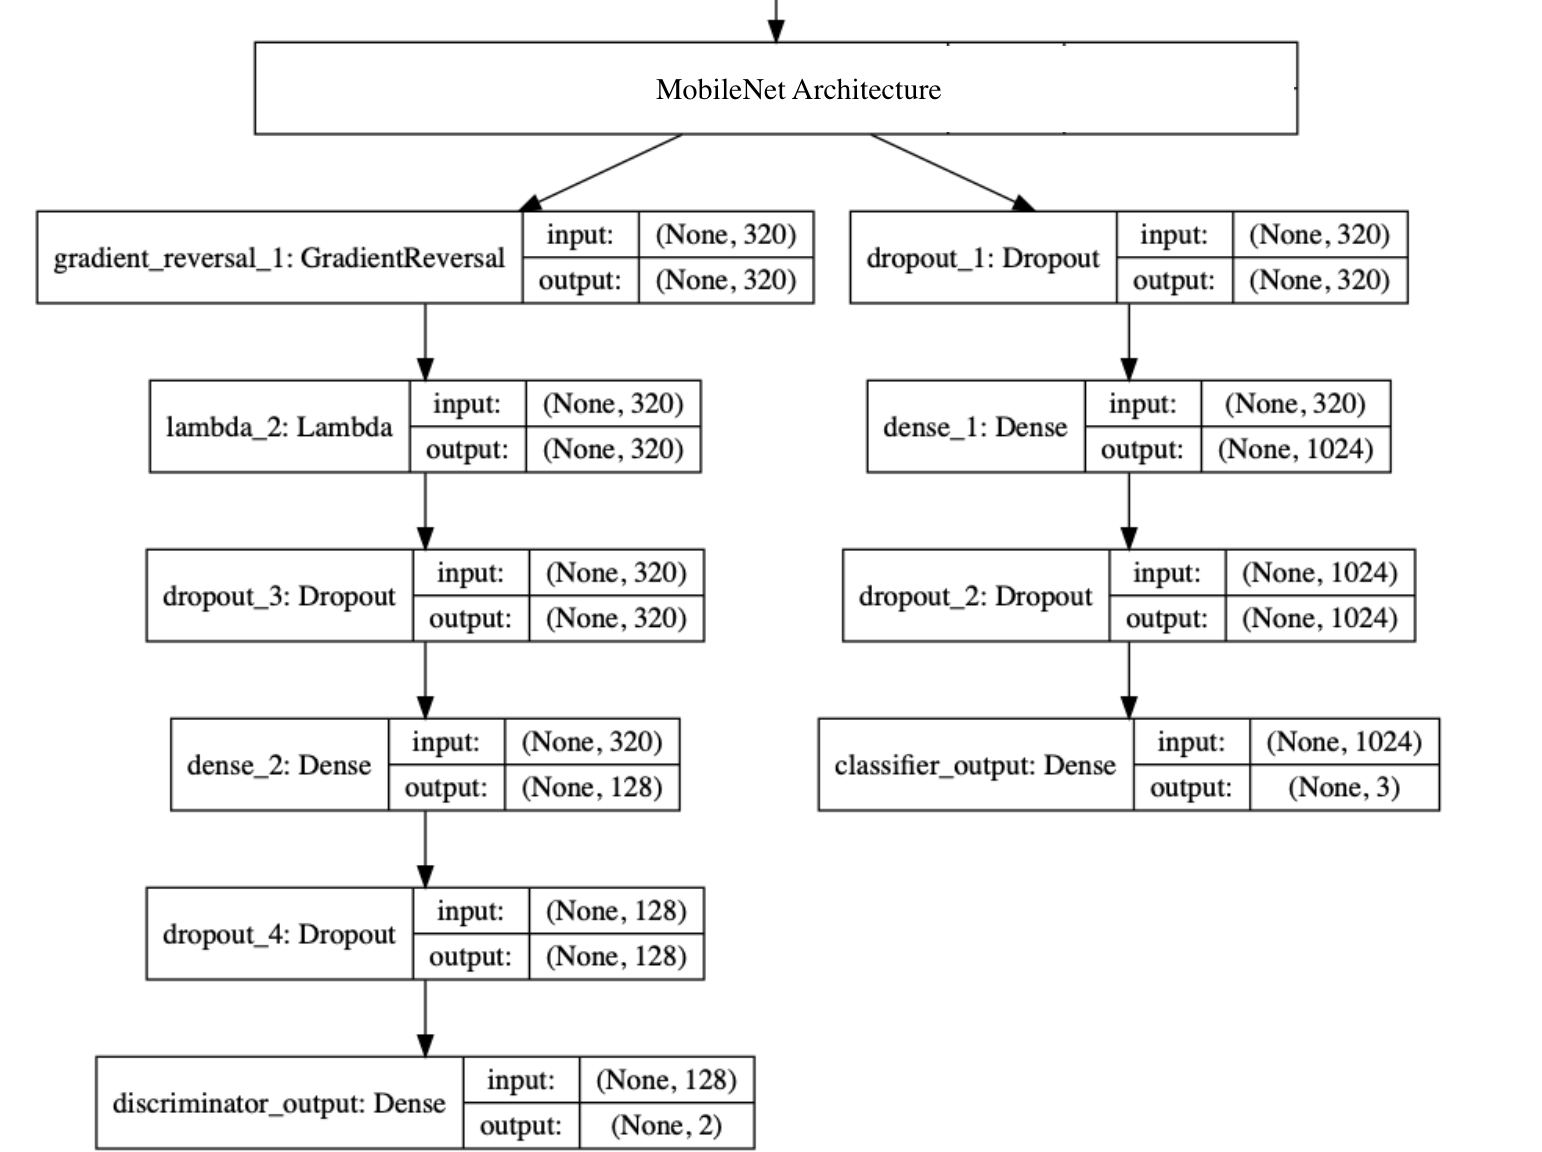
\includegraphics[width=120mm]{Images/Dann_arc.png}
 
 \textbf{Figure 8.} \textit{A diagram showing the added layers to the MobileNet architecture that change the CNN to a DANN CNN, with a gradiant reversal layer for the domain discriminator classifier.}
\end{figure}

If this gradient was zeroed one would be left with a model identical to the classifier discussed previously, based on the MobileNet architecture. If the reversed gradient is not scaled it would have a maximal effect, and would change the weights and biases with an equal effect to the backpropagation from the feature classifier. This would be expected to reduce the effectiveness of the network as the backpropopgation from the domain discriminator would be most destructive in cancelling out the gradients of the feature classifier. In order to assess the effectiveness of a DANN network, a range of linear scaling values, between 0 and 1, were be used to scale the gradient reversal vector.  


\addtocontents{toc}{\vspace{-0.1cm}}
\chapter{Results}
\onehalfspacing

\section{Model Classification}

\subsection{Training on GENIE Dataset}
\noindent After the training process is complete, the model weights and biases are saved to be able to transfer the results of the training to test the trained model on event samples that the network had not seen during the training and validation process. As well as this, statistics from the training and validation process are produced, giving the accuracy and loss values at each epoch. \medskip

\noindent The accuracy is defined as the fraction of the data set that the model correctly classifies, with respect to the truth label. The output of the model, for each event, is a vector with 3 components, much like the shape of the label that was given to the model, However, the result of the network will not be a one-hot encoded vector, but will have the model's confidence in predicting each class- with the model's predicted class being the that the model is most confident in - the vector component with the largest value. As these values represent probabilities of correct classification, the three components will sum to 1.\medskip

\noindent As the weights of the network as initially randomly generated, one would expect it's initial predictions to be poor. As the model is given more training data it can alter these weights to better fit to the data, and thus one would expect the accuracy of the model to increase over time. Similarly, this means that the loss values are expected to decrease over time.\medskip

\noindent Alongside the training accuracy and loss, the validation accuracy loss are given from the training process. These are the values given testing the model on the validation set- containing data not seen in the training process. This process takes place at the end of each training epoch, and no backpropagation takes place, the model is simply used for inference on the data to produce the accuracy and loss values to judge how the model is performing on unseen data, to see whether it is struggling to fit, overfitting, or successfully fitting to the data. \medskip

\begin{figure}[t!]
 \centering
 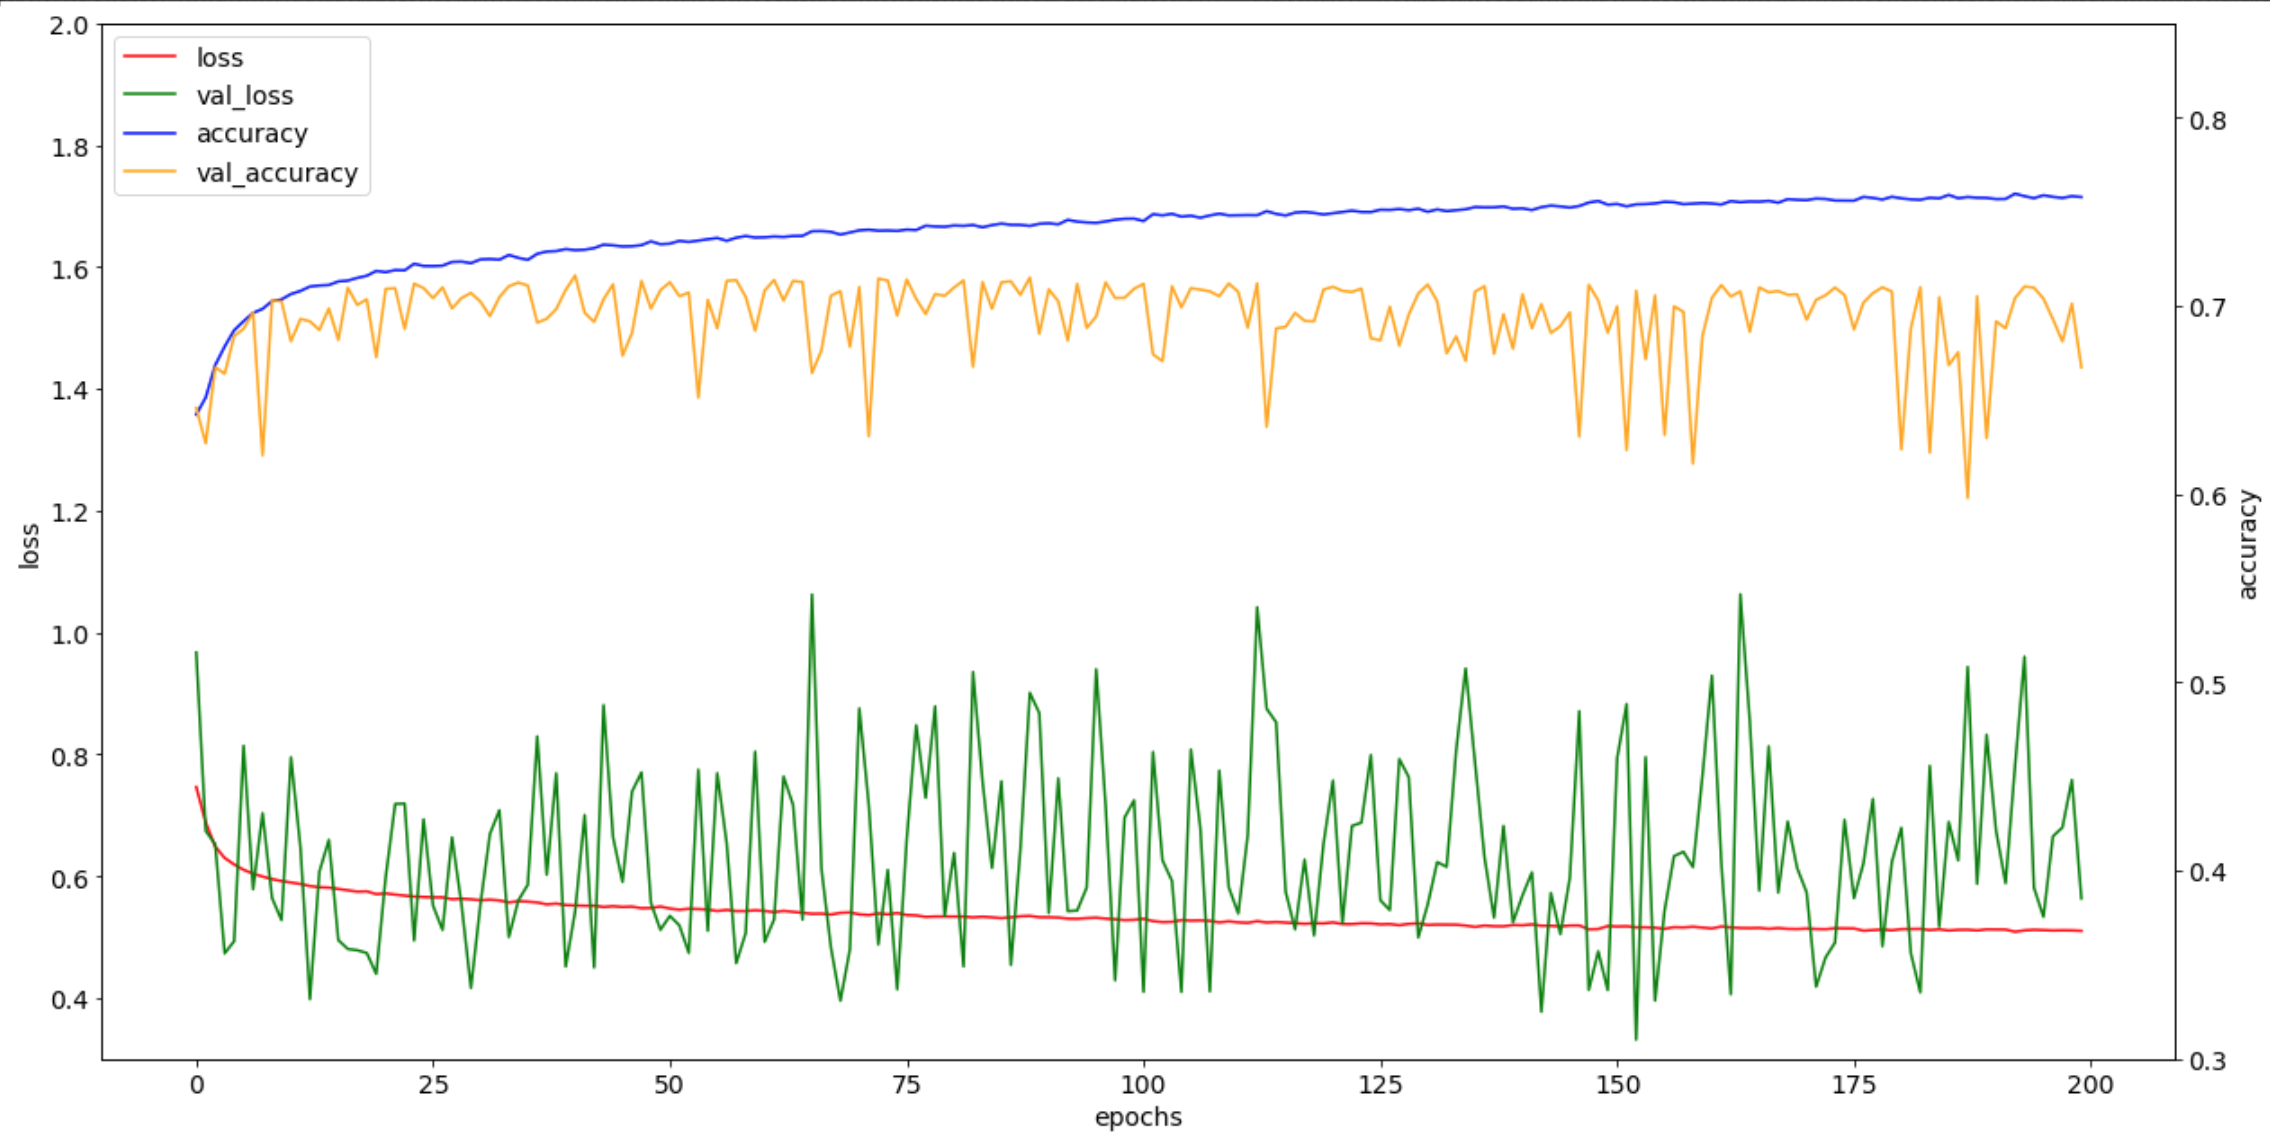
\includegraphics[width=160mm]{genie/acc_loss.png}
 
 \textbf{Figure 9.} \textit{Network training and validation accuracy and loss. The network was trained over 200 epochs using only GENIE generated events. The dateset was not balanced, and the number of $\nu_\mu$ events far exceed that of the other classes. }
\end{figure}

\noindent The MobileNet model was trained on 370864 samples from the GENIE event generator and validated on 52980 samples. The training took place over 200 epochs. As can be seen from the training data, Figure 9, the classifier performs very poorly. The classifier has overfit to the data set, and is struggling to generalise to the unseen validation data, producing the gap between the training accuracy, and the validation accuracy. Unlike traditional overfitting problems where the model overfits by capturing the statistical noise of the data, the overfitting here is taking place due to the data imbalance from the training dataset. In the training dataset, 239932 of the samples were $\nu_\mu$ interactions, 11564 $\nu_e$ interactions, and 119366 NC interactions, and these proportions were mirrored in the validation and testing datasets. Here the classifier can naively predict the event to be a $\nu_\mu$ event every time and be correct 65\% of the time.\medskip

\noindent An ideal classifier will produce two distinct distributions, whereby it can confidently predict the correct classification, and also confidently classify those that are of the the other classes- ie a very low prediction probability of $\nu_e$ or NC events when the truth value is a $\nu_\mu$ event. In Figure 10, it can be seen that a large number of $\nu_\mu$ events are accurately predicted with a high probability, however, the truth $\nu_e$ and NC events are also being classified as $\nu_\mu$ events. This classifier has struggled to determine the differences between the different classes. This can also be seen in Figure 11, where the $\nu_e$ classifier correctly identified $\nu_\mu$ and NC events as not $\nu_e$ events with a high probability, however it is classifying every event as a $\nu_\mu$, and thus no events as $\nu_e$ interactions, and incorrectly classifying the $\nu_e$ events.\medskip

\noindent In this case it is redundant to look at the purity and the efficiency of the classifier as every event is being classifier as as $\nu_\mu$ event, giving the classifier a very high efficiency, as all the $\nu_\mu$ events are identified correctly, however the purity of the classifier is poor as events that are not $\nu_\mu$ events are being classified as so. \medskip

\begin{figure}[t!]
 \centering
 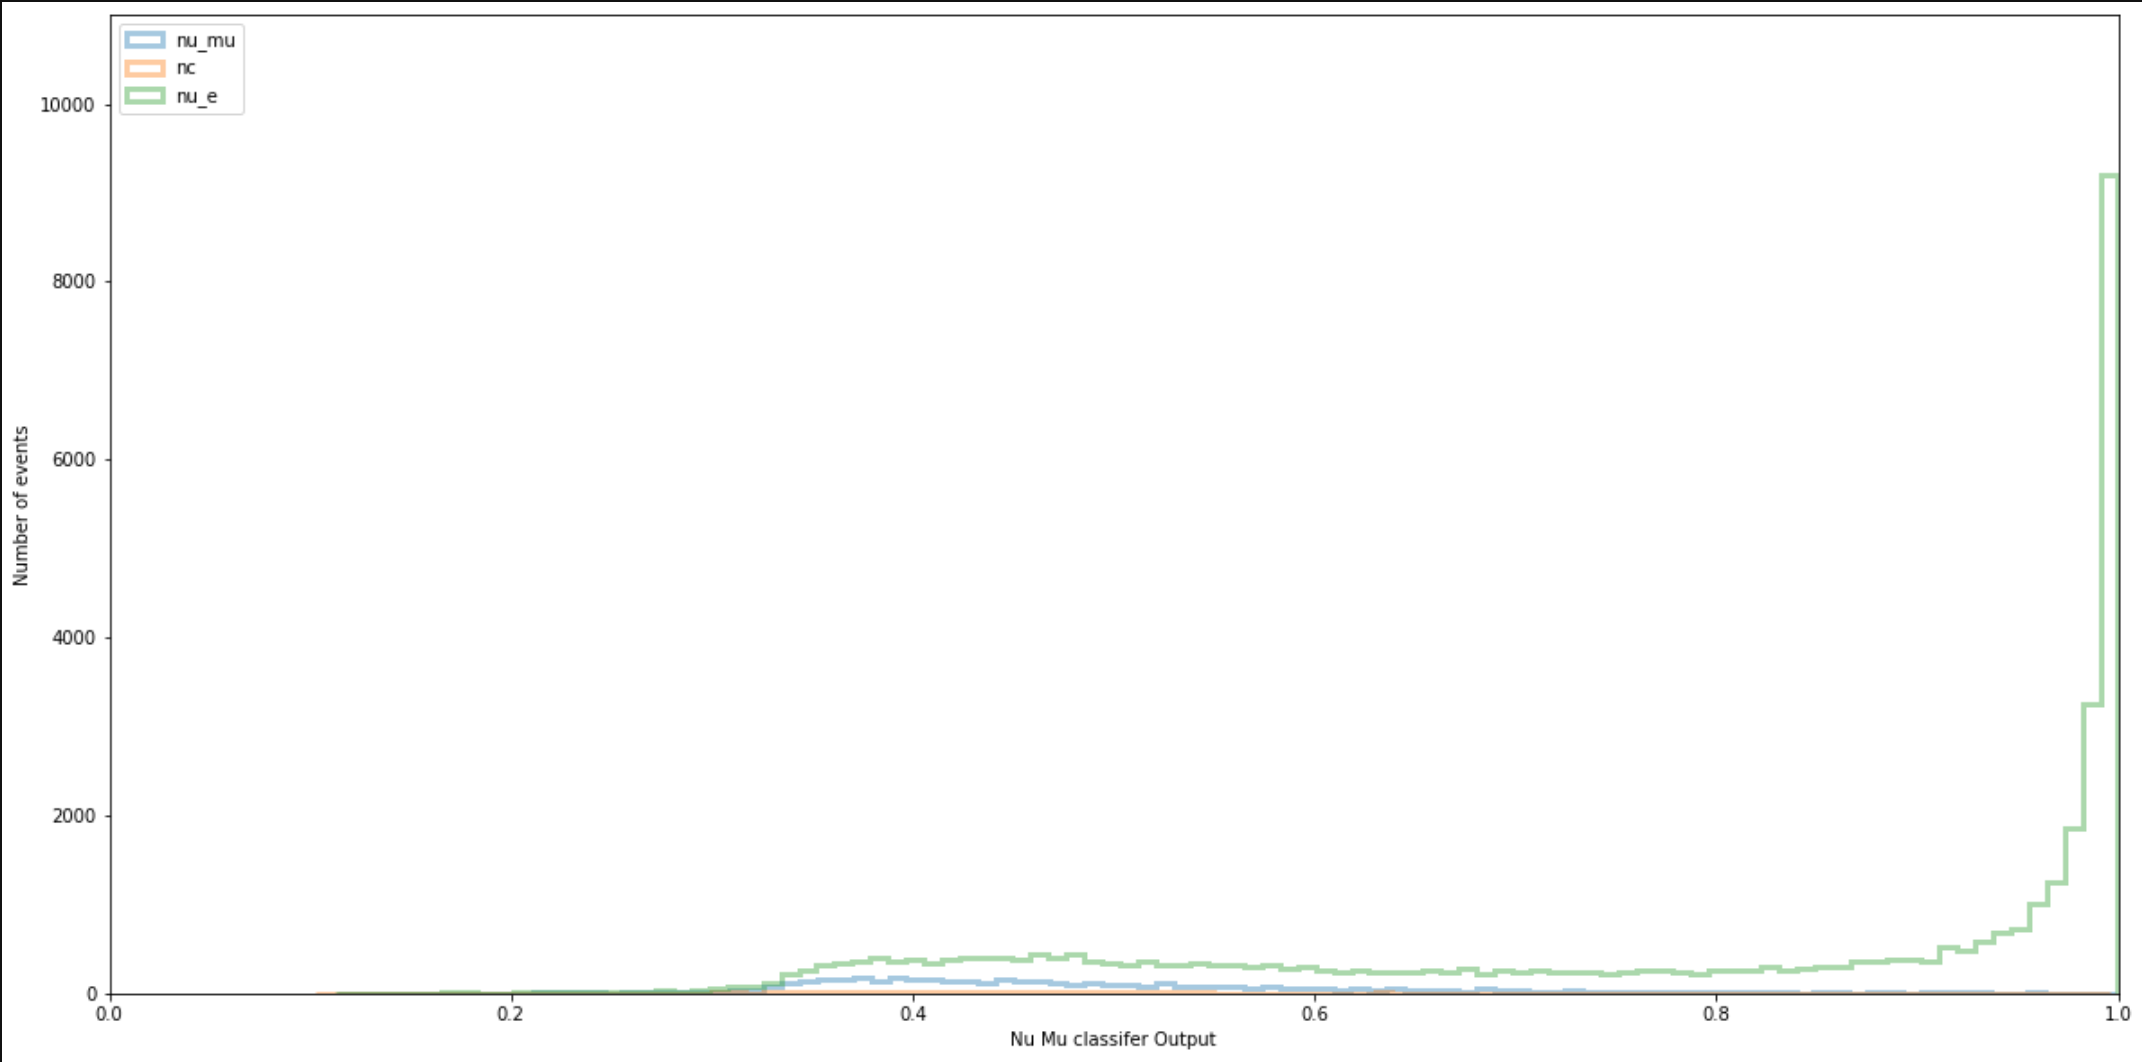
\includegraphics[width=160mm]{genie/NUMU.png}
 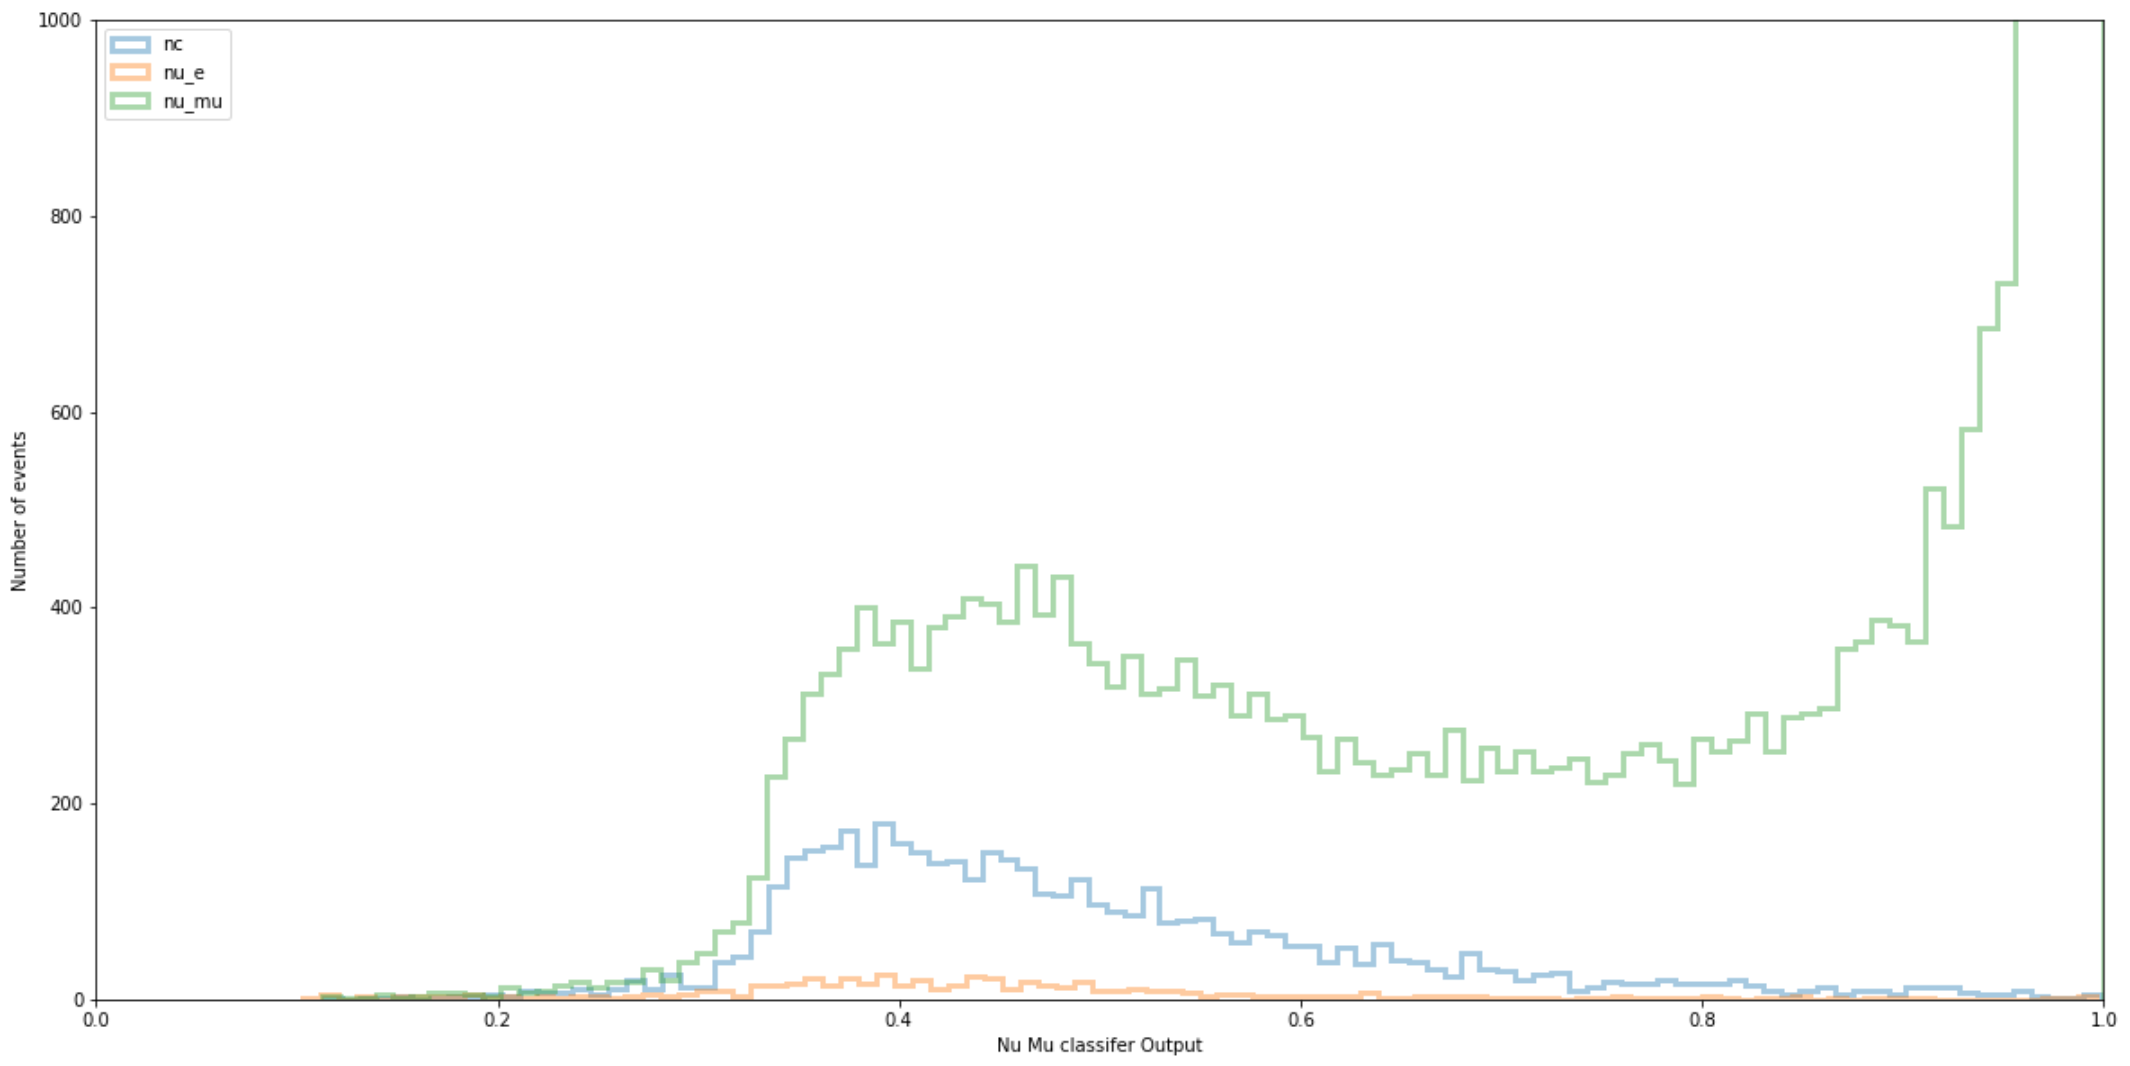
\includegraphics[width=160mm]{genie/NUMUZOOM.png} 
 
 \textbf{Figure 10.} \textit{$\nu_\mu$ classification output histogram. The dataset was trained and tested using only GENIE generated events. The dateset was not balanced, and the number of $\nu_\mu$ events far exceed that of the other classes.  Figures show the probability of being classified a $\nu_\mu$ for events of all the interaction types. Top Figure shows the entire dataset, while the bottom Figure shows a cropped version of the same dataset with the axis limited to a reduced number of counts.}
\end{figure}

\begin{figure}[t!]
 \centering
 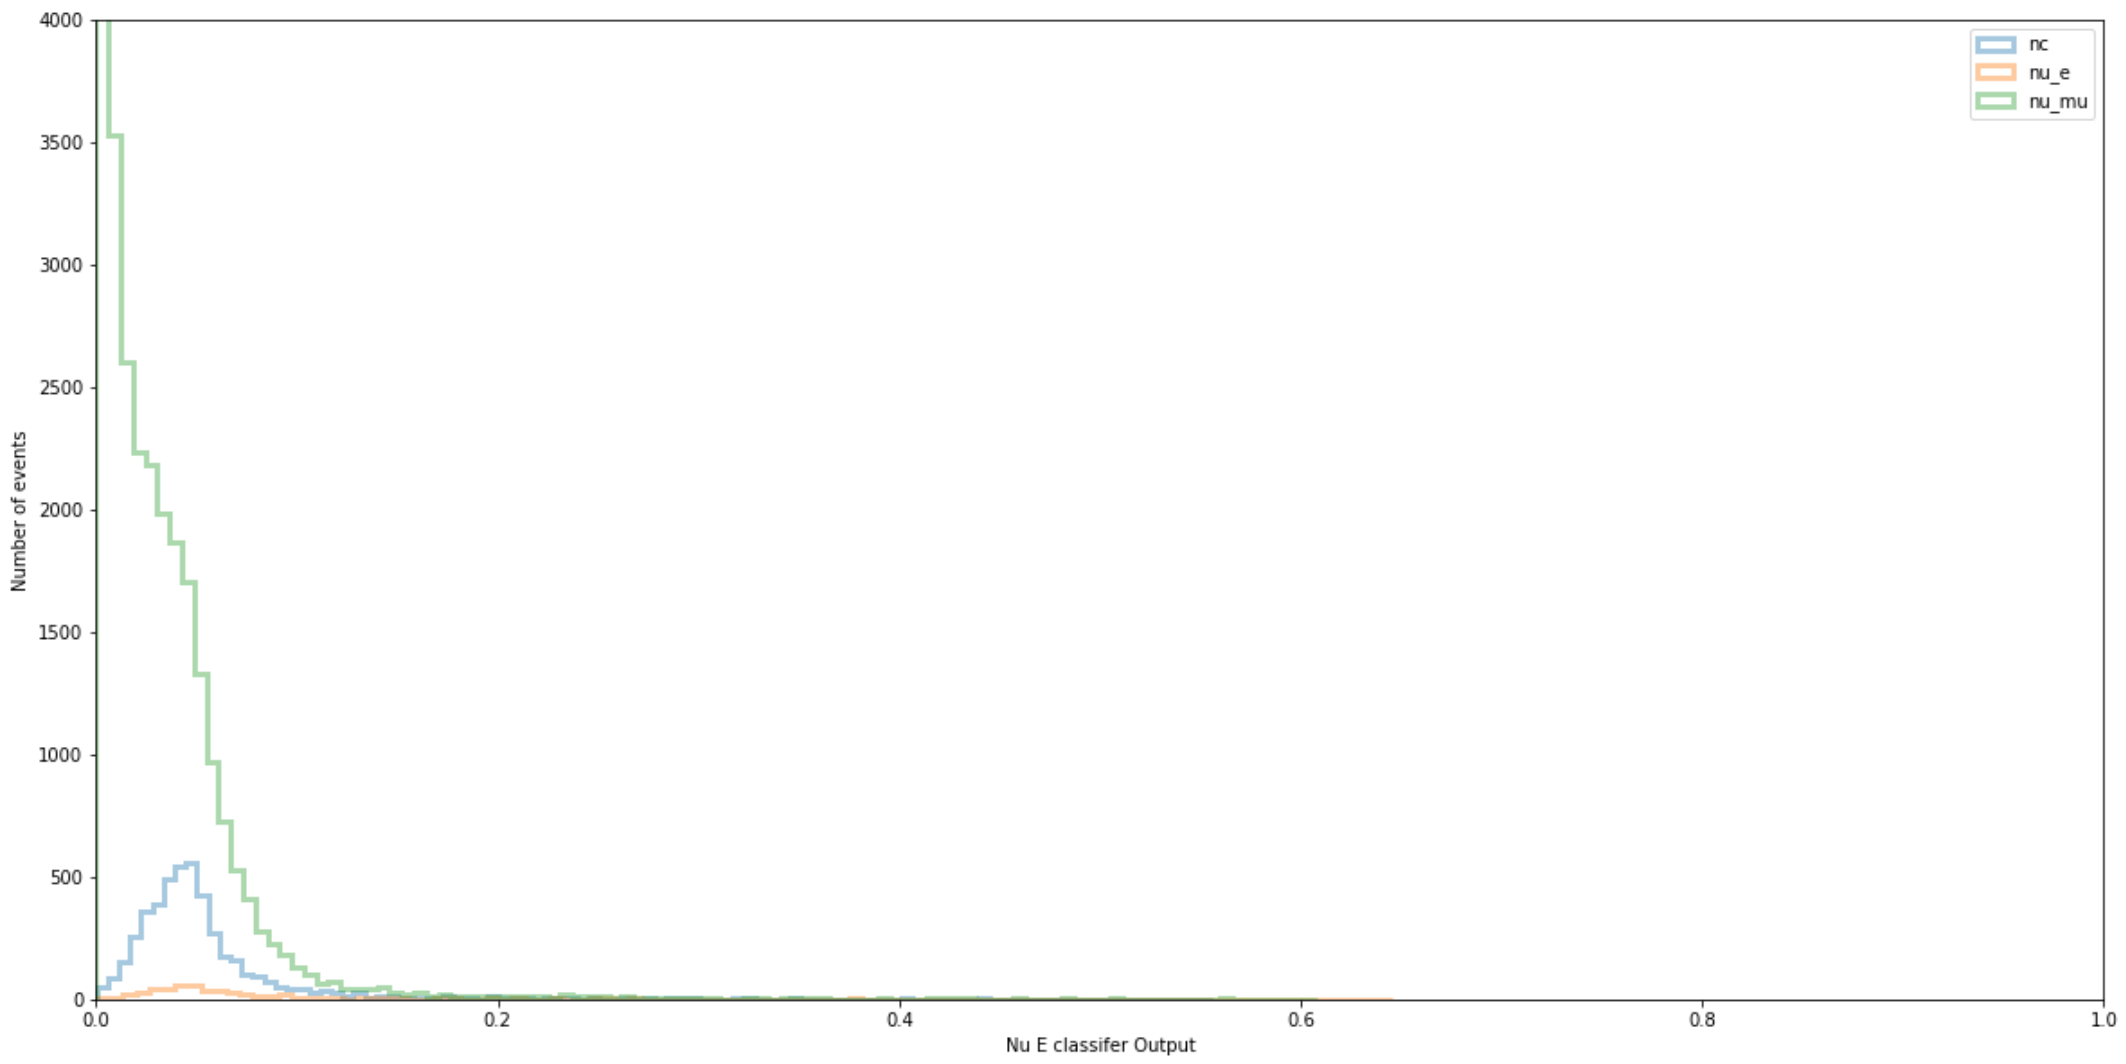
\includegraphics[width=160mm]{genie/NUE.png}
 
 \textbf{Figure 11.} \textit{$\nu_e$ classification output histogram. Figures show the probability of being classified a $\nu_\mu$ for events of all the interaction types. The training process was the same as for that in Figure 10.}
\end{figure}



 
\input{3.1.2 Results} 
\subsection{Training on a balanced GENIE Dataset and evaluated on GiBUU Data}

\noindent In order to see if there was a bias in the training process the model previously described in the previous section was used to classify GiBUU events. As the model had previously been trained on GENIE only events, if the classification results of GiBUU were poorer, we could establish that the model had become too specific to GENIE dataset and that there were differences in how the GENIE and GiBUU simulated these events. \medskip

\begin{figure}[t!]
 \centering
 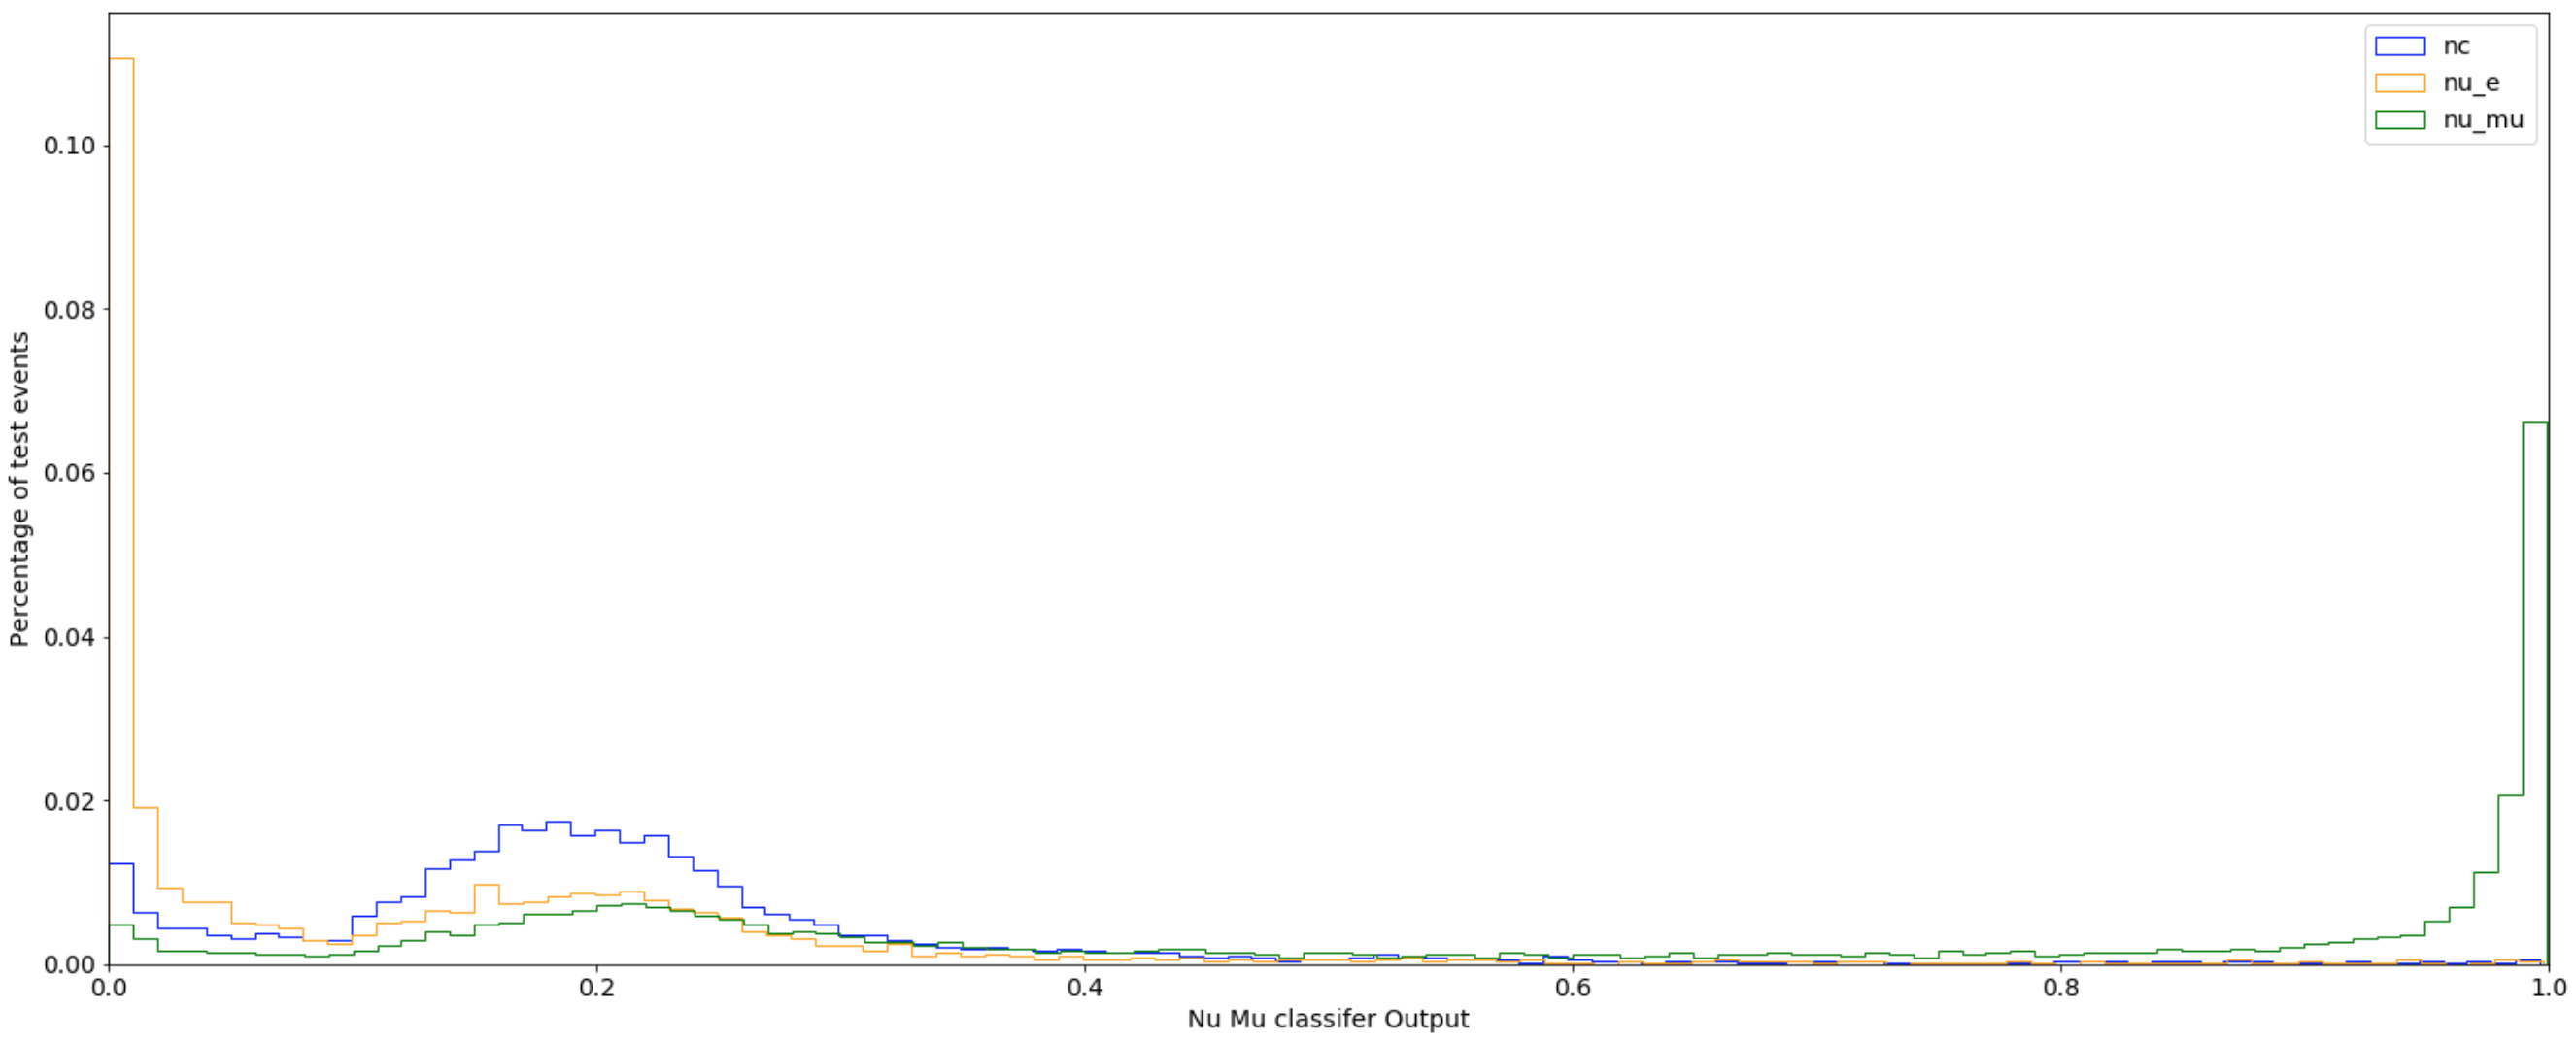
\includegraphics[width=160mm]{genie/gibuu/numu.png}
 \textbf{Figure 17.} \textit{$\nu_\mu$ classification output histogram. The dataset was trained using balanced GENIE only events- the same training process as the model in figures 13 and 14, but was evaluated on a balanced GiBUU dataset. Figures show the probability of being classified a $\nu_\mu$ for events of all the interaction types.}

 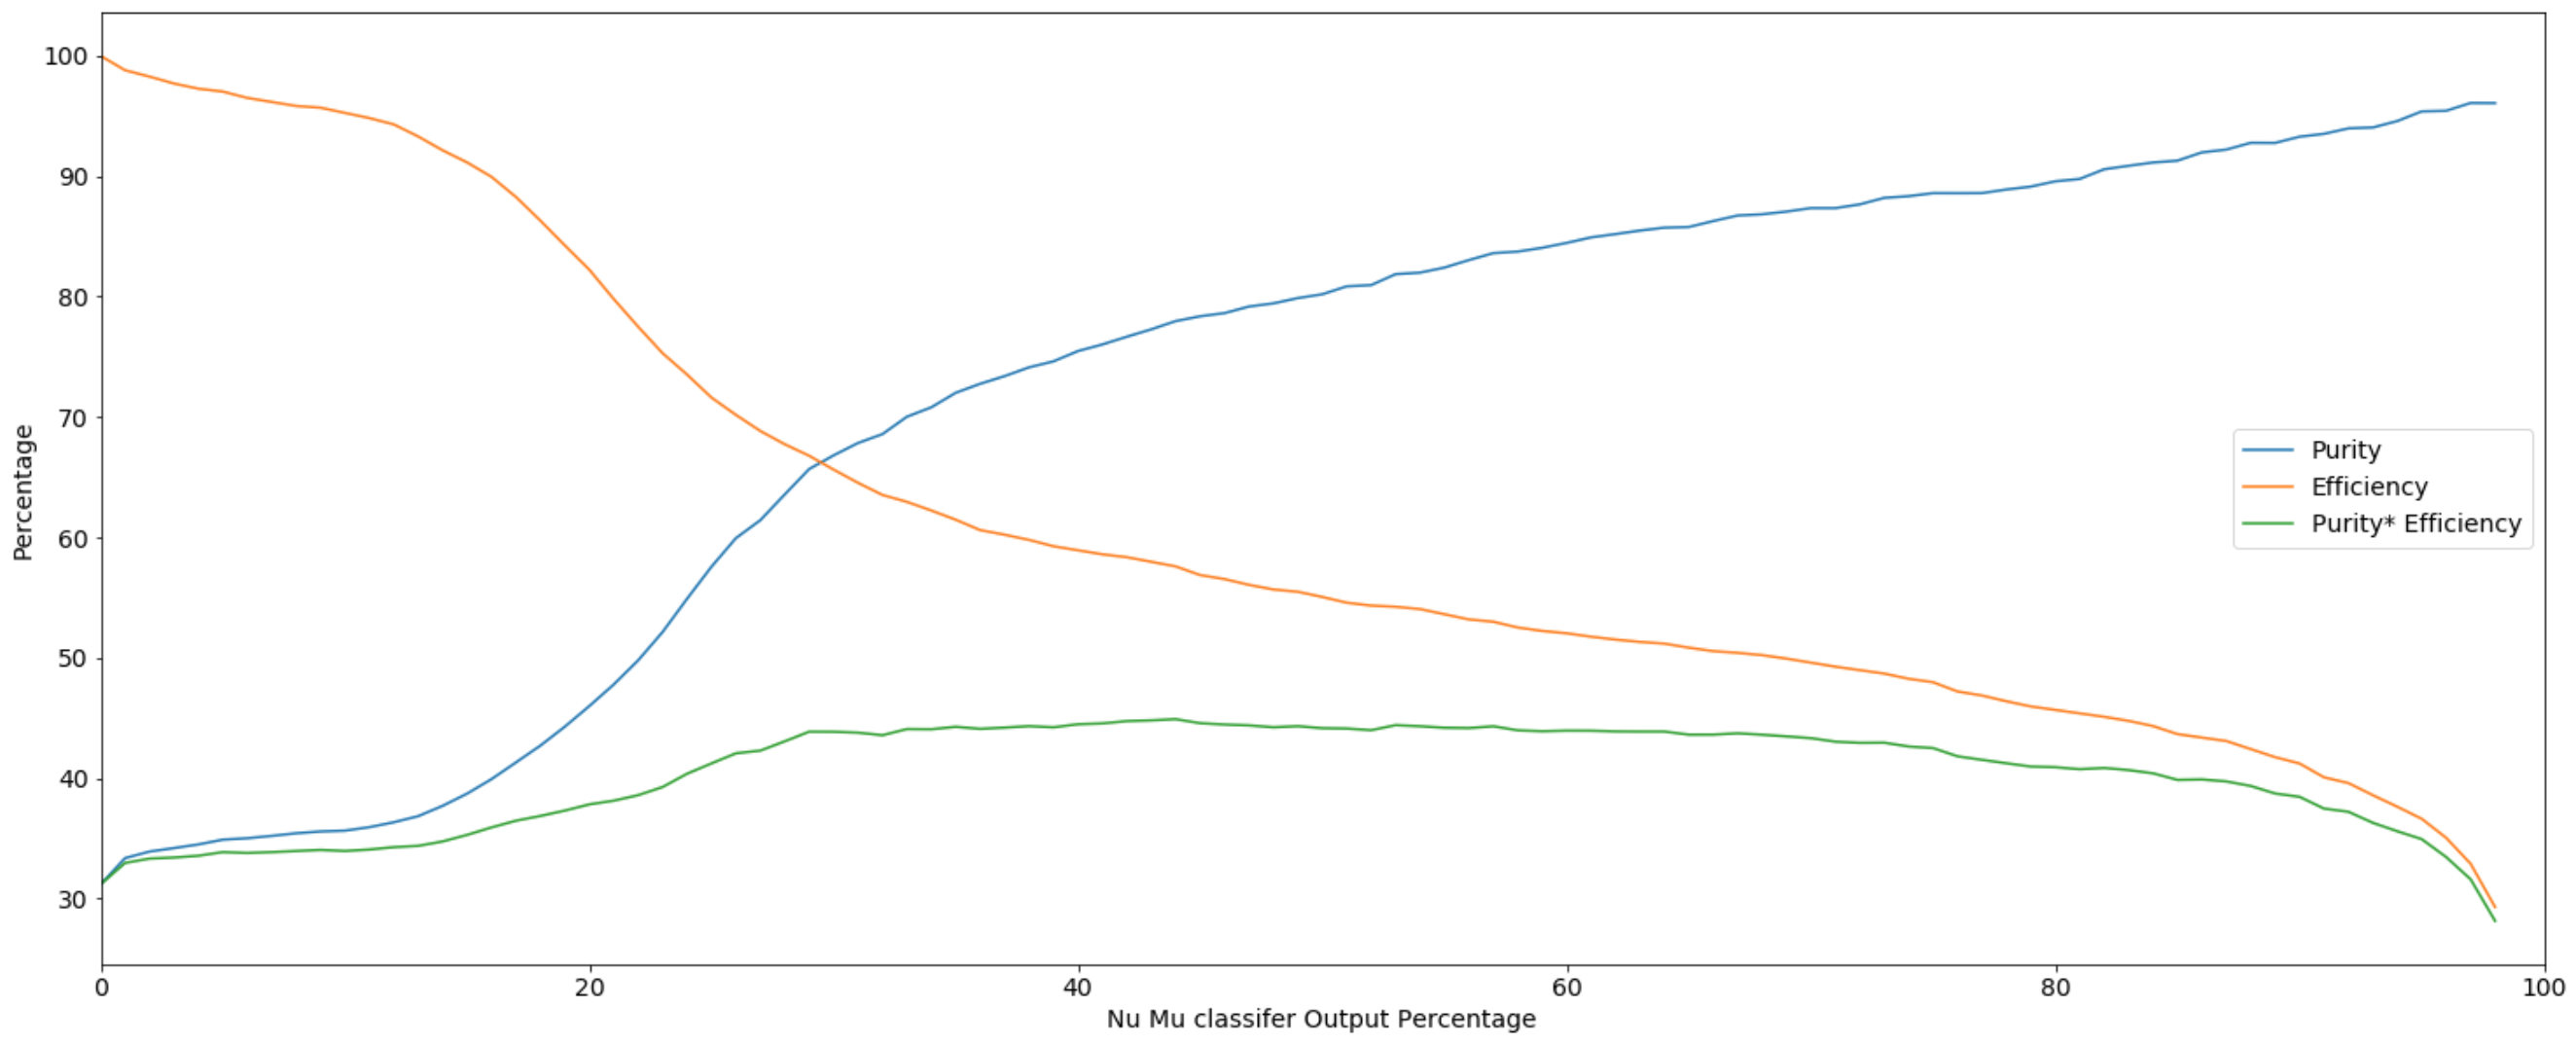
\includegraphics[width=160mm]{genie/gibuu/numupe.png}
 \textbf{Figure 18.} \textit{$\nu_e$ classification output histogram. The dataset was trained using balanced GENIE only events- the same training process as the model in figures 13 and 14, but was evaluated on a balanced GiBUU dataset. Figures show the probability of being classified a $\nu_e$ for events of all the interaction types.}
\end{figure}

\noindent The classifier was tested on 8856 events produced by GiBUU with an equal number of each of the interaction types. The $\nu_\mu$ classifier performs similarly when tested on GiBUU events as to when tested on GENIE events, with a similar proportion of events being correctly classified with a confidence level of above 90\%, this can be seen by comparing Figures 17 and 13. The difference between the two classification results is that at at confidence levels between 10\% and 30\%, see Figure 17, all three event types can be seen to be classified with similar confidence levels by the model with a similar distribution. Due to this mis-classification of $\nu_\mu$ events, the efficiency curve in Figure 18 falls steeply over this model output range, but then flattens out, as very few events are classified with a confidence between 30 and 80\%. This may be because the GiBUU generator produces a class of each event that look similar to the others. This is unusual as we would expect some $\nu_\mu$ and $NC$ events to look similar, and some $\nu_e$ and $NC$ events to look similar, but not $\nu_\mu$ and $\nu_e$ events to do so. \medskip

\begin{figure}[t!]
 \centering
 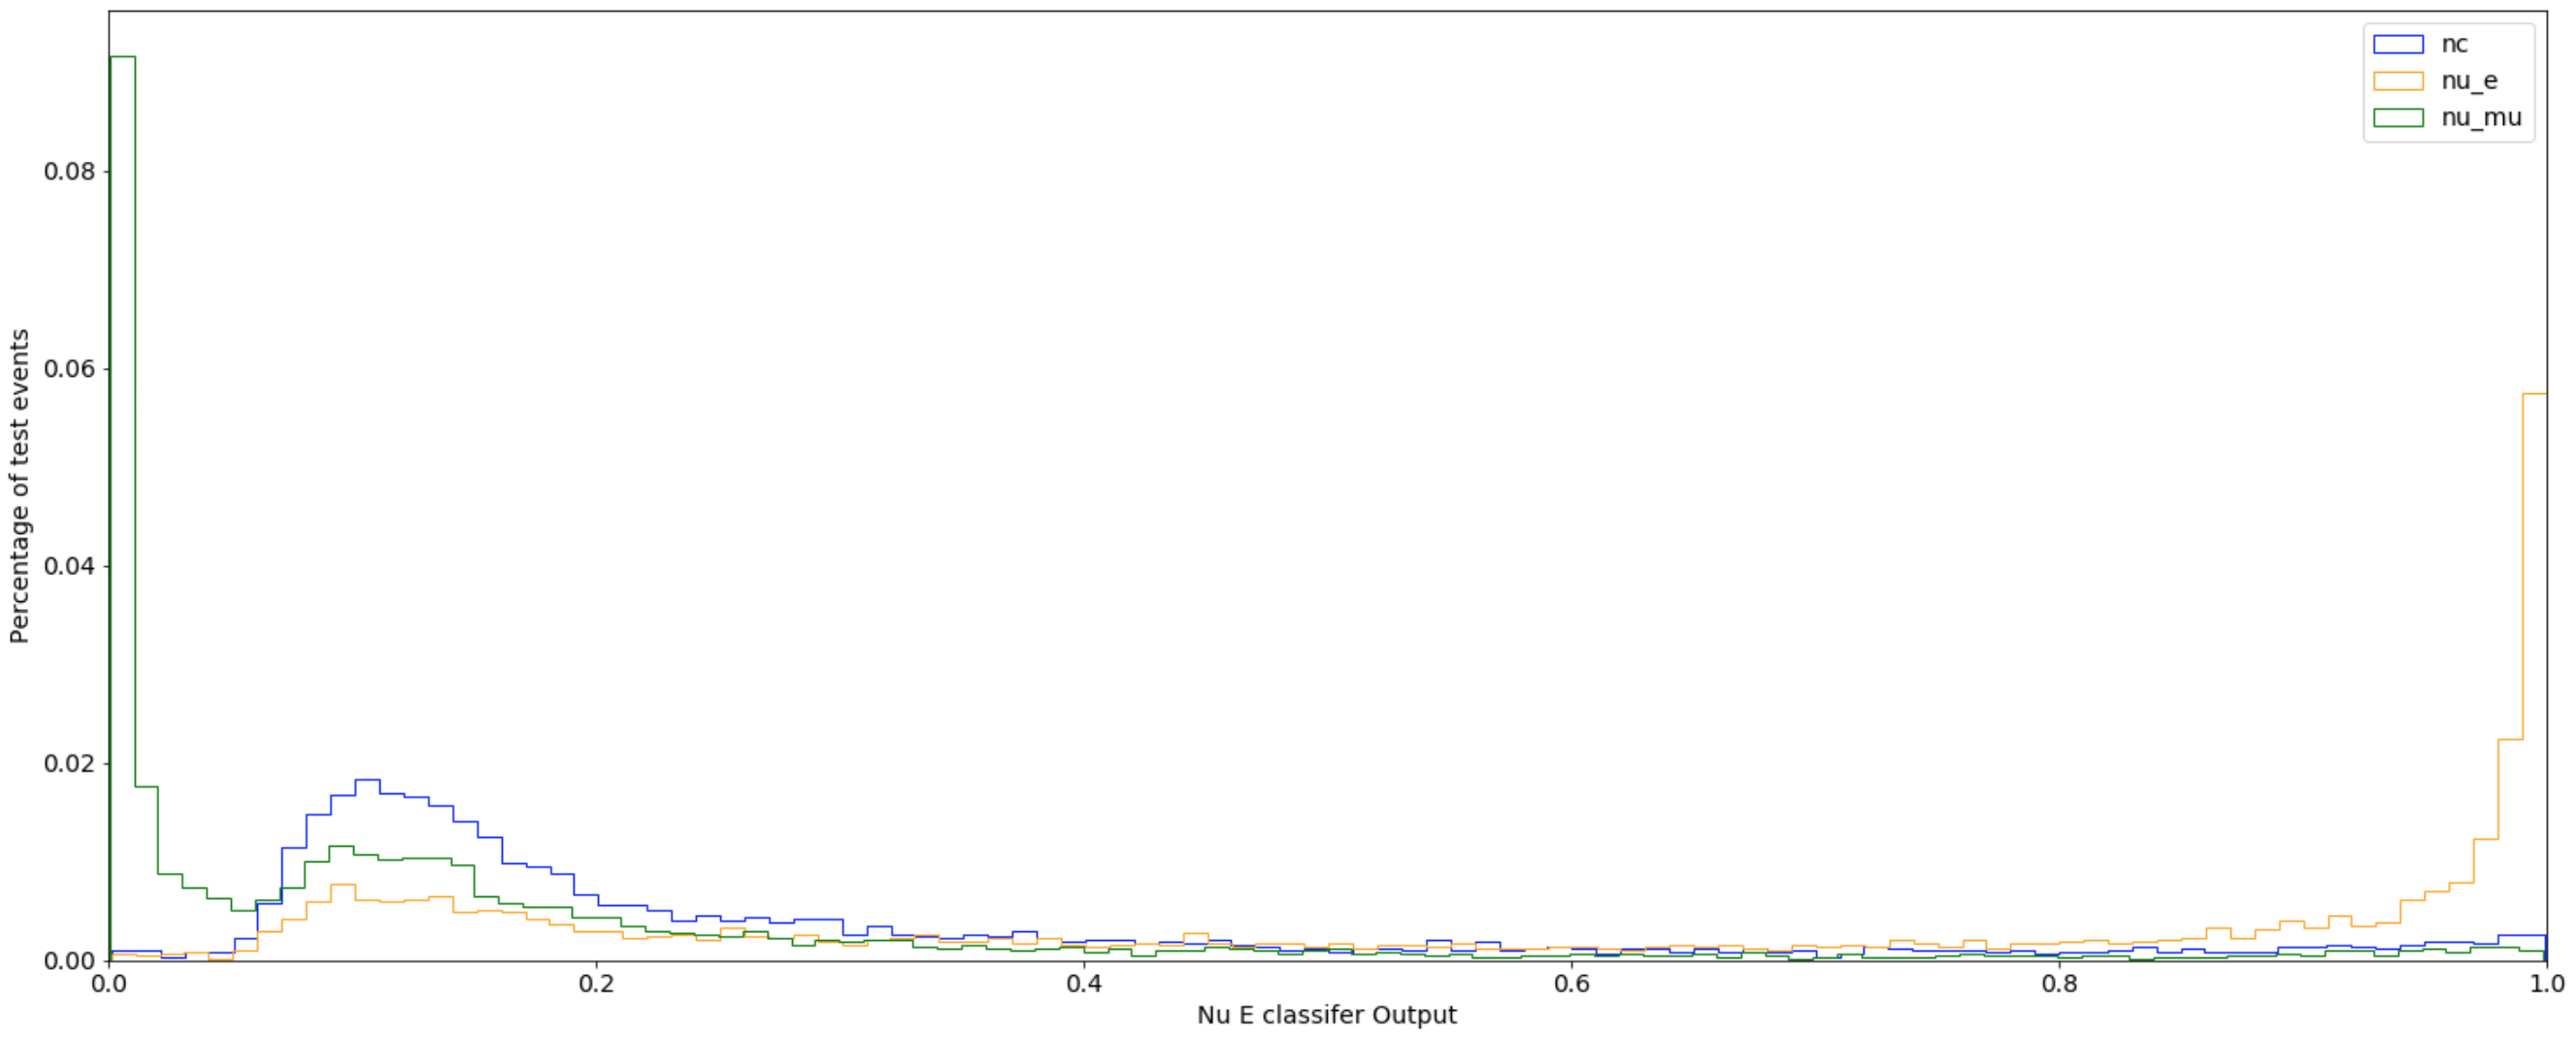
\includegraphics[width=160mm]{genie/gibuu/nue.png}
 \textbf{Figure 19.} \textit{Purity, efficiency and their product, curves for the $\nu_\mu$ classifier trained on a balanced GENIE dataset and tested on a balanced GiBUU dataset. The x-axis shows the confidence percentage of the network out (output multiplied by 100 to give the percentage).}

 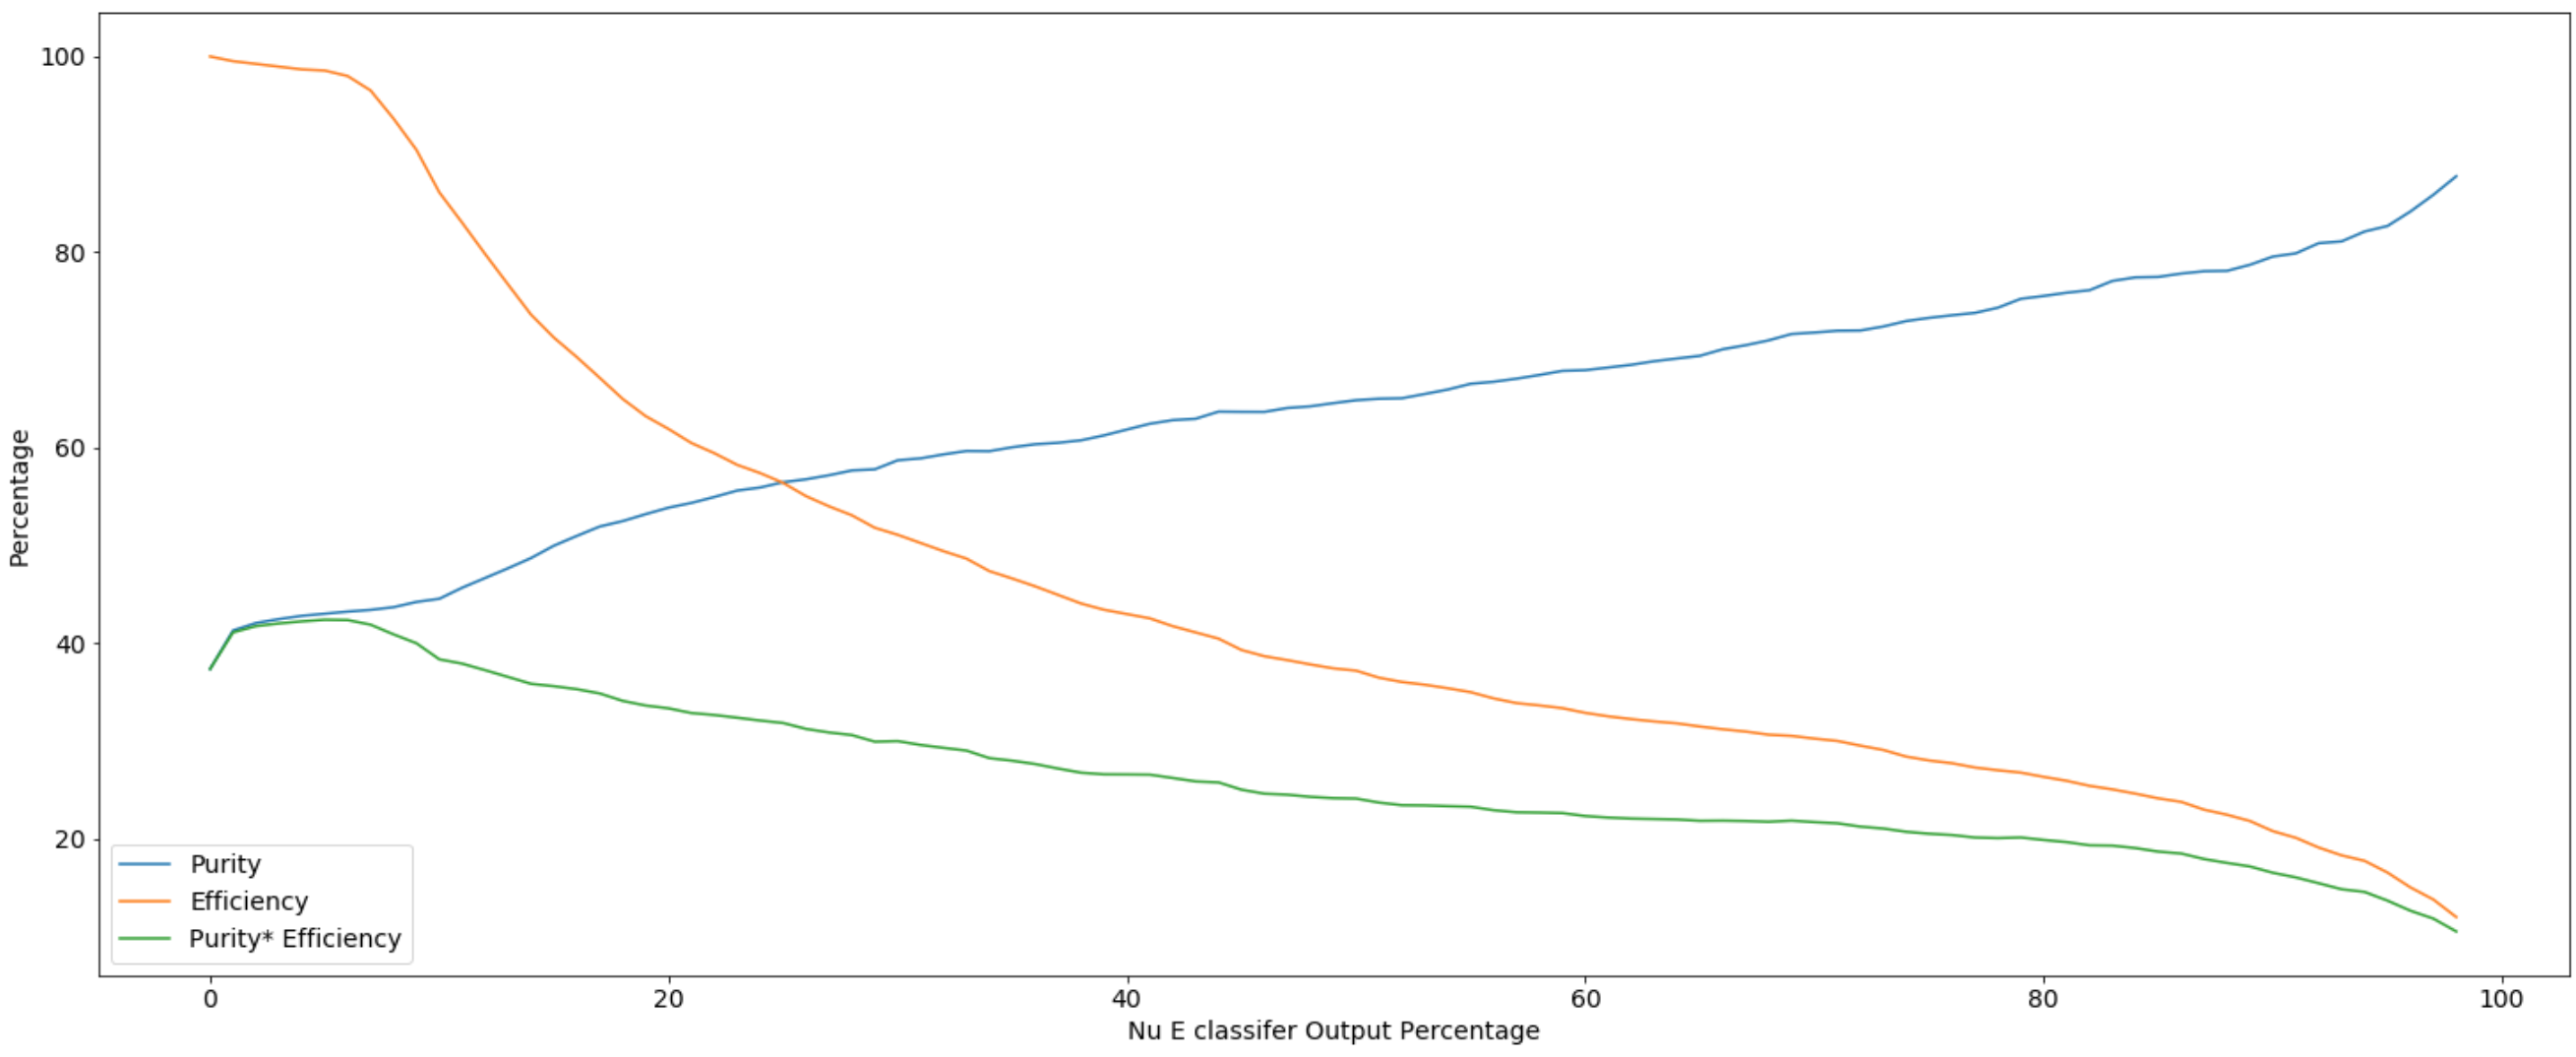
\includegraphics[width=160mm]{genie/gibuu/nuepe.png}
 \textbf{Figure 20.} \textit{Purity, efficiency and their product, curves for the $\nu_e$ classifier trained on a balanced GENIE dataset and tested on a balanced GiBUU dataset.}
\end{figure}

\noindent Looking at the classification of the $\nu_e$ events produced by GiBUU in Figure 19, we see that the model is not as strong in classifying events produced by GiBUU compared to produced by GENIE for the GENIE trained model. A similar proportion of the event samples were confidently correctly classified as $\nu_e$ events with a confidence of 90\% and above. The model also correctly classifies $\nu_\mu$ events as not $\nu_e$ with a high level of confidence, however the proportion of such events is smaller in the GiBUU dataset than the GENIE testing dataset. A reason for this is likely the slightly lower confidence classification of $\nu_\mu$ events, as well as $NC$ and $\nu_e$ events between 5\% and 25\% confidence levels. As with the $\nu_\mu$ classifier, the similarity in the distribution of confidence levels for the three interaction types in this confidence range is very similar, and indicates some similarity that the model is unable to discern between these events. As there are a larger number of $\nu_e$ events are wrongly classified with a high confidence, the efficiency curve in Figure 20 falls very steeply, resulting in a poor purity efficiency product curve compared to Figure 16. \medskip 
\subsection{Training on both GENIE and GiBUU Data}

\noindent A model was trained on both the GENIE and GiBUU datasets, and contained 61,804 samples for training, 8,830 for validation and 17,658 for testing with an equal number of the 3 interaction types, and an equal number of GENIE and GiBUU generated events.\medskip

\begin{figure}[t!]
 \centering
 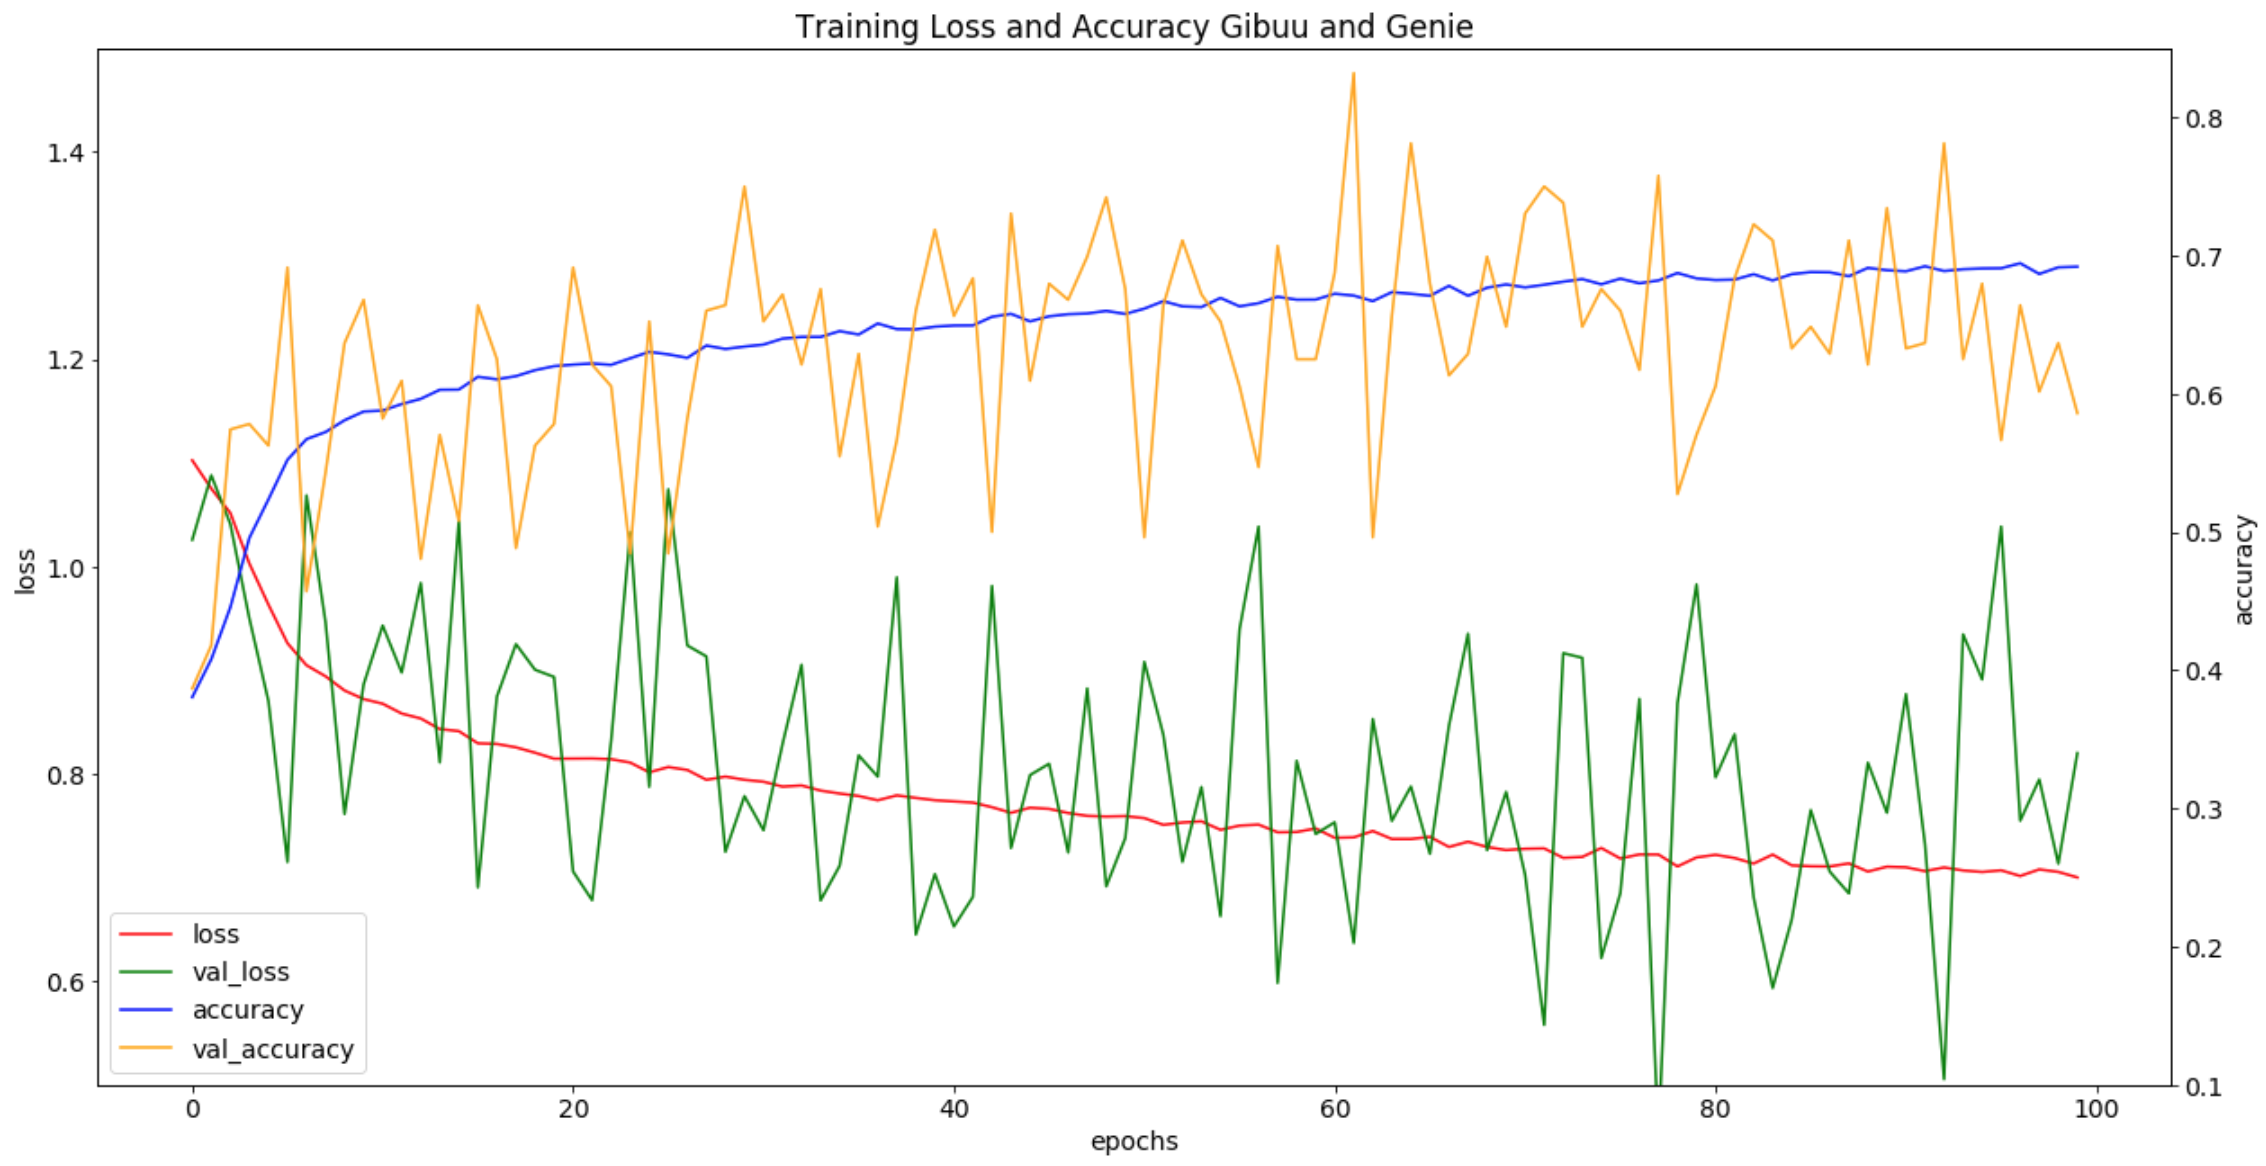
\includegraphics[width=160mm]{Both_Data/train.png}
 \textbf{Figure 21.} \textit{Network training and validation accuracy and loss.The network was trained over 100 epochs using both GENIE and GENIE generated events. With an equal number of all three event types. }
\end{figure}

\noindent From the training statistics in Figure 21, we can see that the model does not over fit the same way the imbalanced dataset did. The validation set often performs better than the training process, and this is because during the training process the dropout function is applied, so that network is classifying based on only a subset of its architecture. When then validating, all the nodes in the model are now available producing a more powerful classifier. The validation set also performs more poorly than the testing set during some epochs of the process, and this is because the network has over fit to the data it has seen and does not generalise as well to the unseen data. Overtime these two processes oscillate, however the overall trend of performance is increasing, as is expected.\medskip

\noindent Looking at the $\nu_\mu$ classifier output, Figure 22, we can see that the network performs well- better than the classifier that was trained on only GENIE events. The $\nu_\mu$ classifier successfully classifies a large proportion of the truth $\nu_\mu$ events correctly with a confidence of 90\%, while successfully classifying nearly all of the truth NC events as not $\nu_\mu$ with a confidence level of 60\% and $\nu_e$ with a confidence of 80\%. A number of truth $\nu_\mu$ events are predicted as not $\nu_\mu$ with a similar probability as the NC events, and this may be cause they are the subset of the $\nu_\mu$ that appear most similar to NC events, this will be looked into further in the Domain Classification section.\medskip

\begin{figure}[t!]
 \centering
 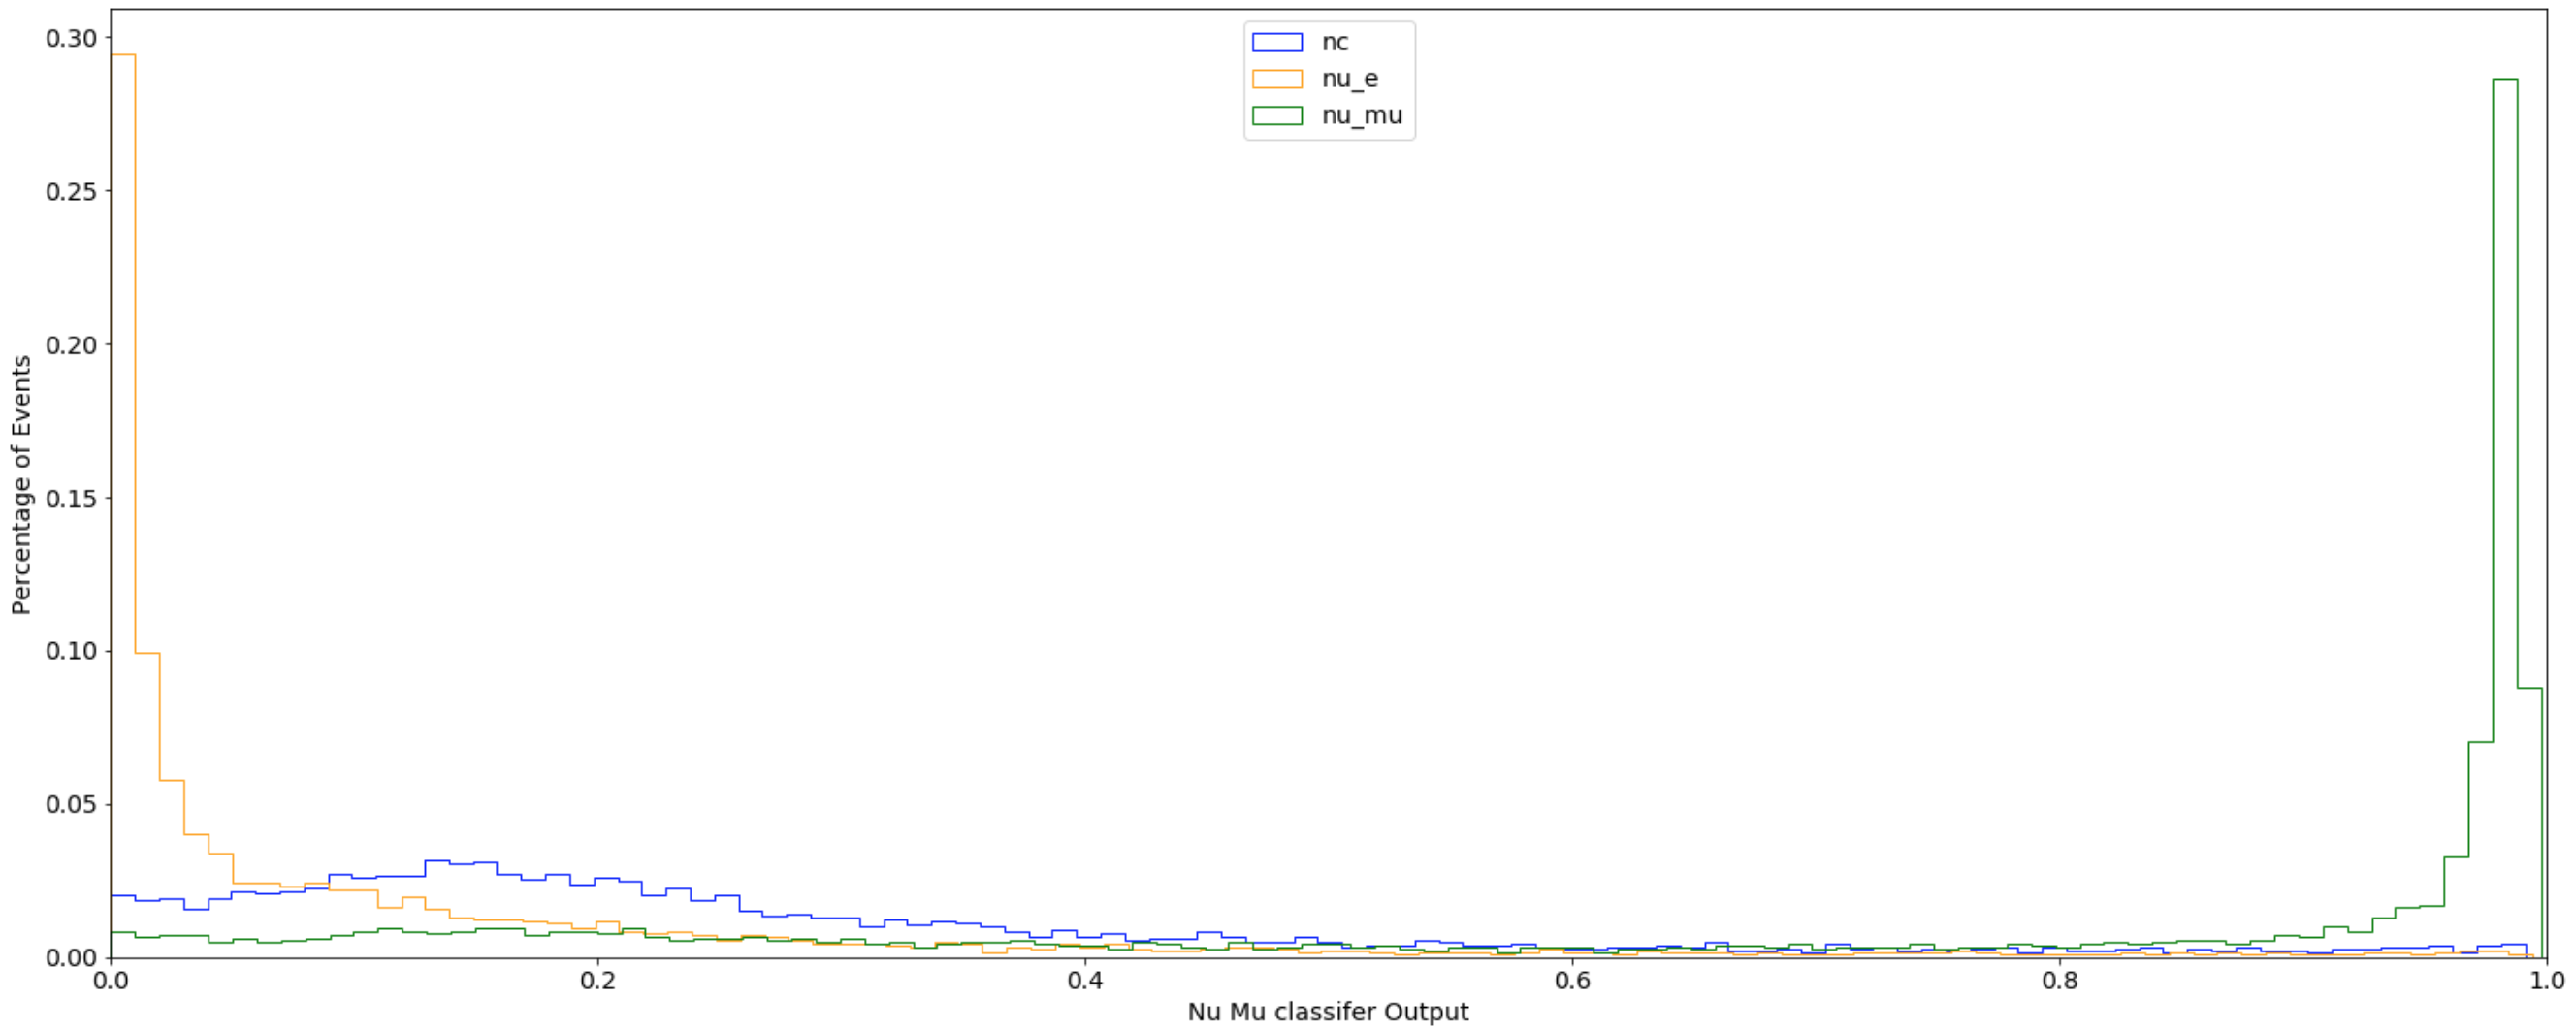
\includegraphics[width=160mm]{Both_Data/NUMU.png}
 \textbf{Figure 22.} \textit{$\nu_\mu$ classification output histogram. The dataset was trained and tested using data from both GENIE and GIBUU generated events. The dataset contained an equal number of all three event types.}

 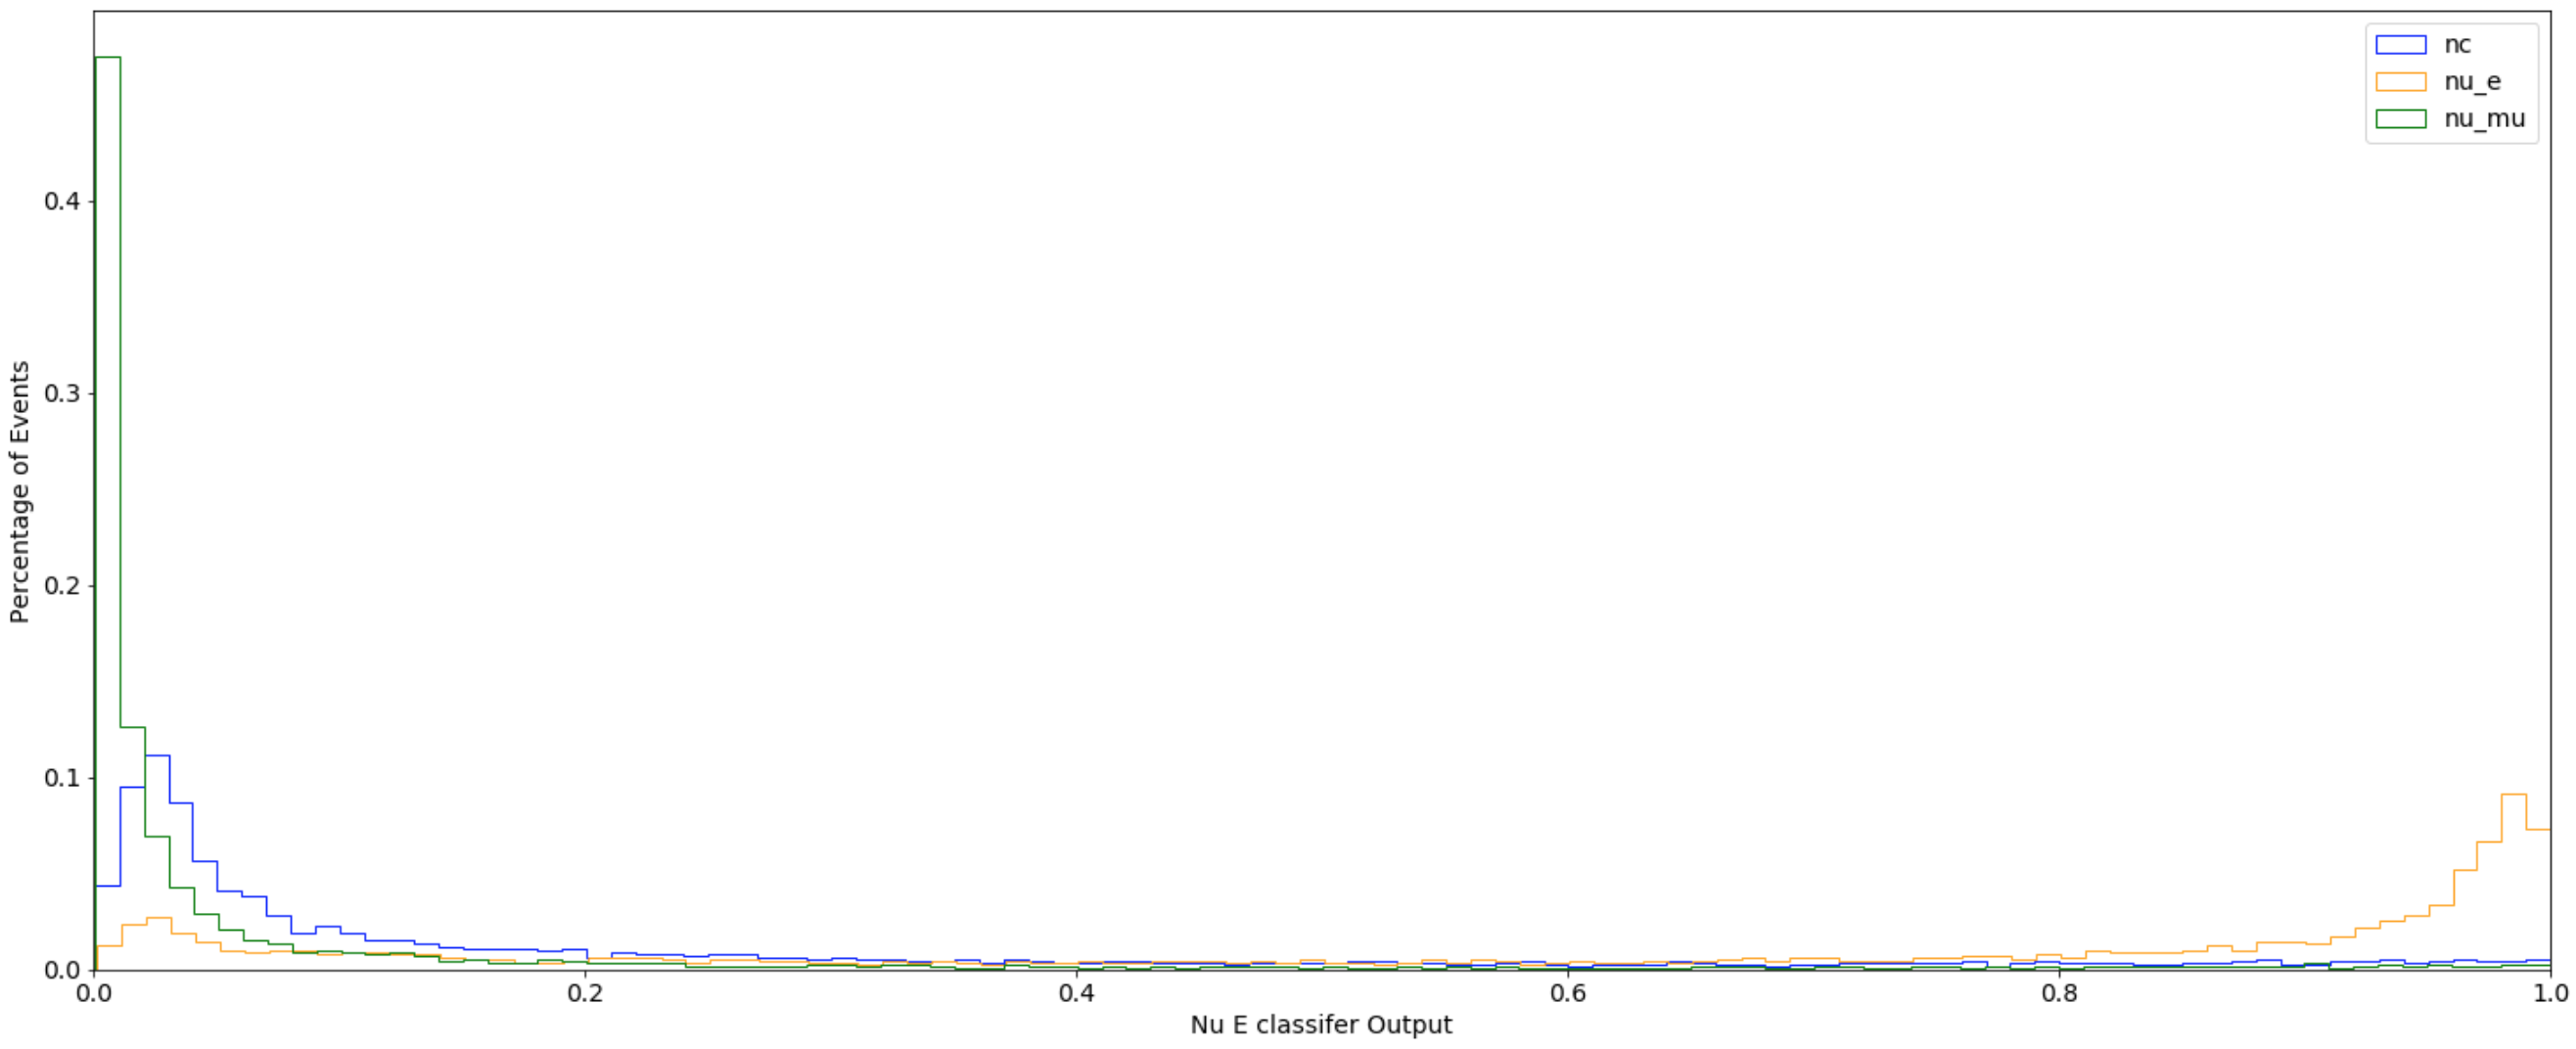
\includegraphics[width=160mm]{Both_Data/NUE.png}
 \textbf{Figure 23.} \textit{$\nu_e$ classification output histogram. The results were produced from the same training and testing process as Figures 21 and 22.}
\end{figure}

\noindent The $\nu_e$ classifier, in Figure 23, does not perform as strongly as the $\nu_\mu$ classifier, with a much smaller proprtion being correctly identified as $\nu_e$ events with a confidence of 80\%. What the $\nu_e$ does well is that it is able to correctly identify events as not $\nu_e$ events, with a large proportion of the $\nu_\mu$ and $NC$ events being classified as not $\nu_e$ events with a confidence level of 90\%. What also can be seen is again a number of $\nu_e$ are incorrectly identified as not $\nu_e$ with a similar confidence distribution as the $NC$ events, and this may be as these are the $\nu_e$ events that look similar to the $NC$ events that have large showers. \medskip

\begin{figure}[t!]
 \centering
 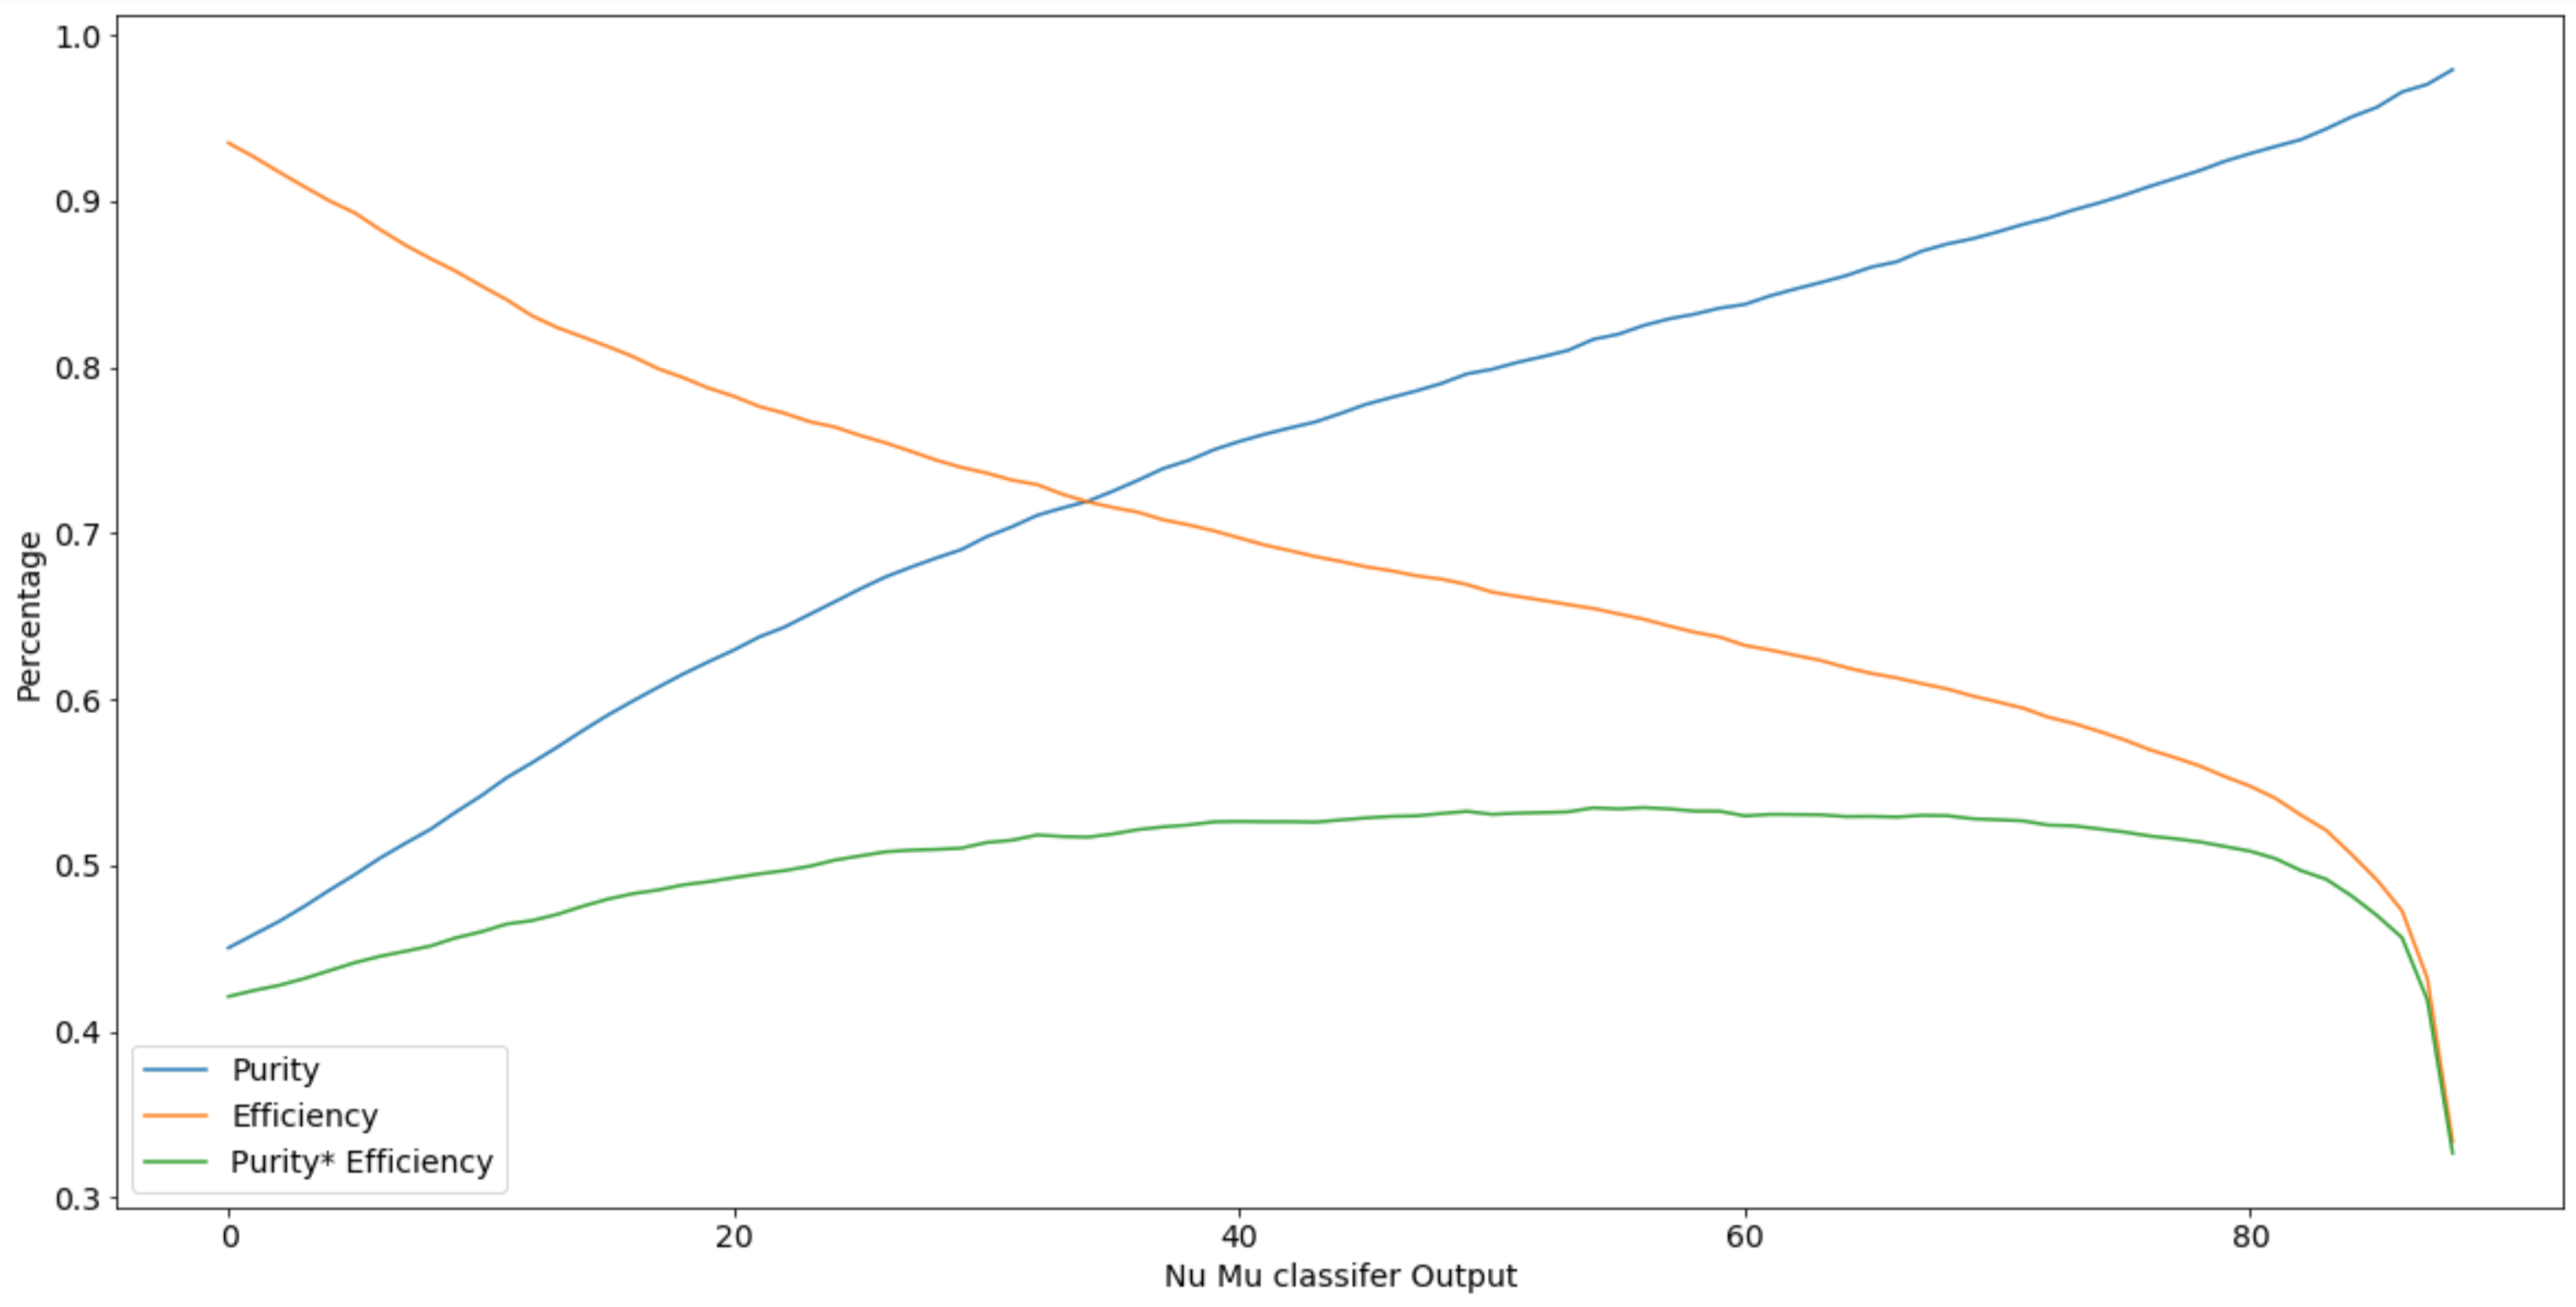
\includegraphics[width=160mm]{Both_Data/NUMUCL.png}
 \textbf{Figure 24.} \textit{$\nu_\mu$ classification output purity, efficiency and their product. The results were produced from the same training and testing process as Figures 22 and 23.}
 
 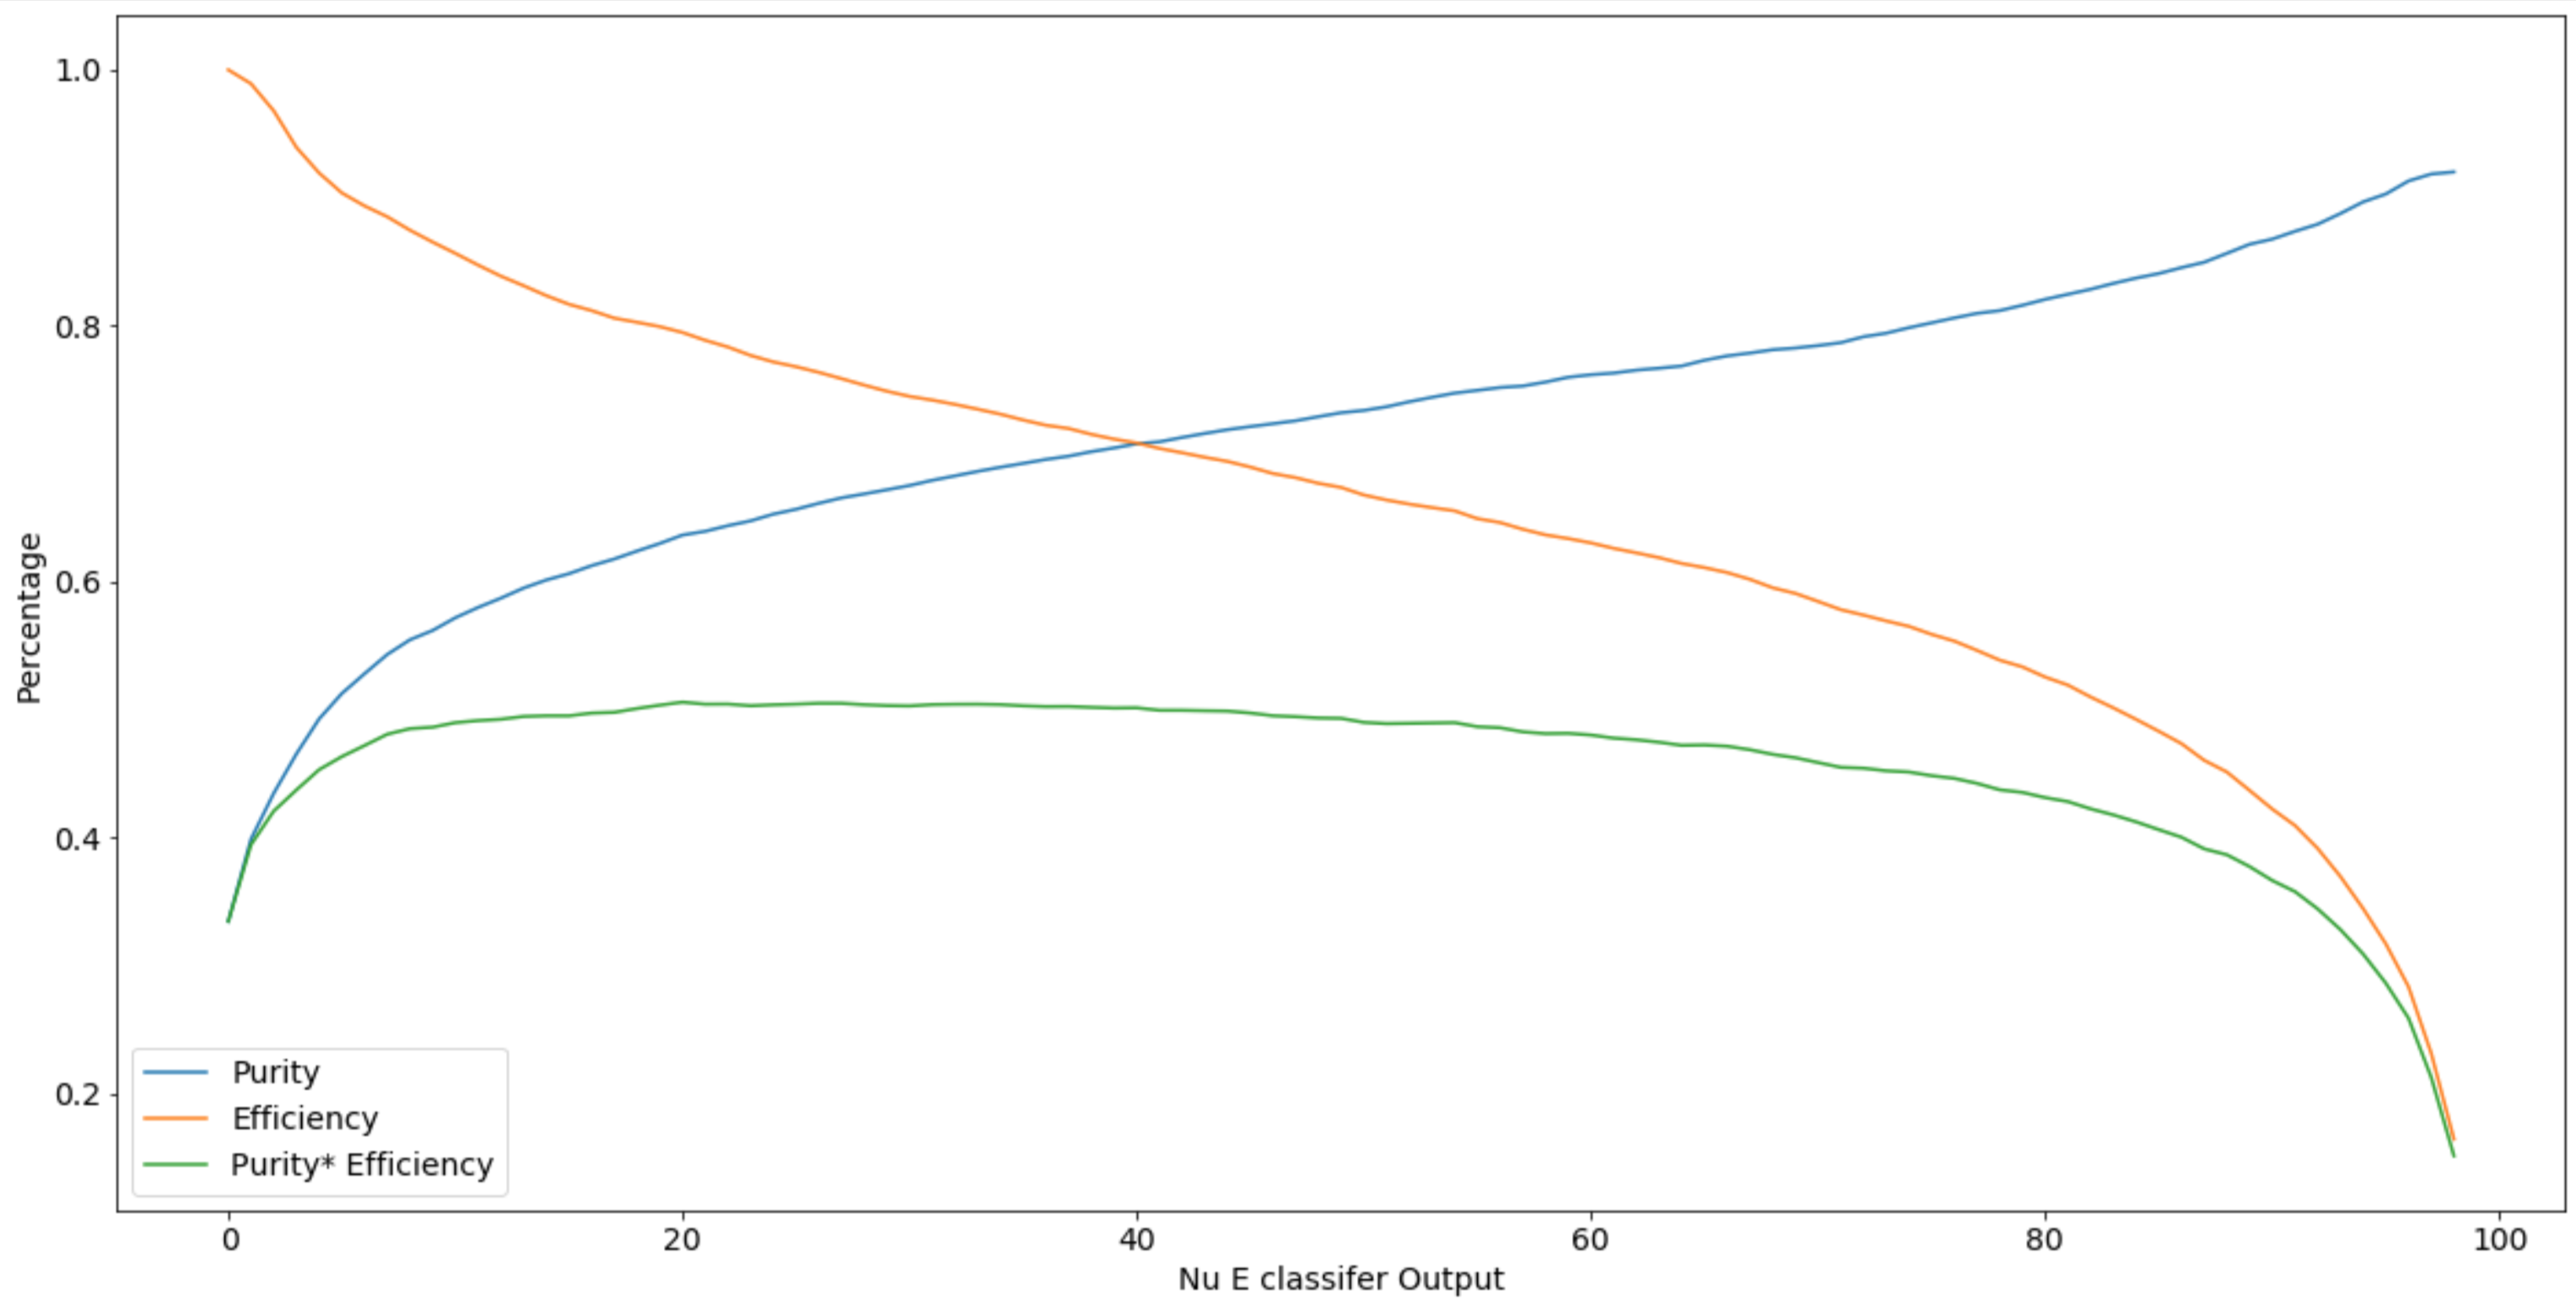
\includegraphics[width=160mm]{Both_Data/NUECL.png}
 \textbf{Figure 25.} \textit{$\nu_e$ classification output purity, efficiency and their product. The results were produced from the same training and testing process as Figures 22 and 23.}
\end{figure}


\noindent By looking at the $\nu_\mu$ purity-efficacy plot in Figure 24 and $\nu_e$ plot in Figure 25, it can be seen that the $\nu_\mu$ purity-efficiency product curve confirms the better performance that was indicated in Figure 22. The selection cut for the $\nu_\mu$ classifier would be made at a might higher value than with the $\nu_e$ classifier, and a cut at a 60\% confidence value would provide a classification accuracy, given by the purity value of 82\% while retaining 62\% of the $\nu_\mu$ events. \medskip

\begin{figure}[t!]
 \begin{subfigure}{}
 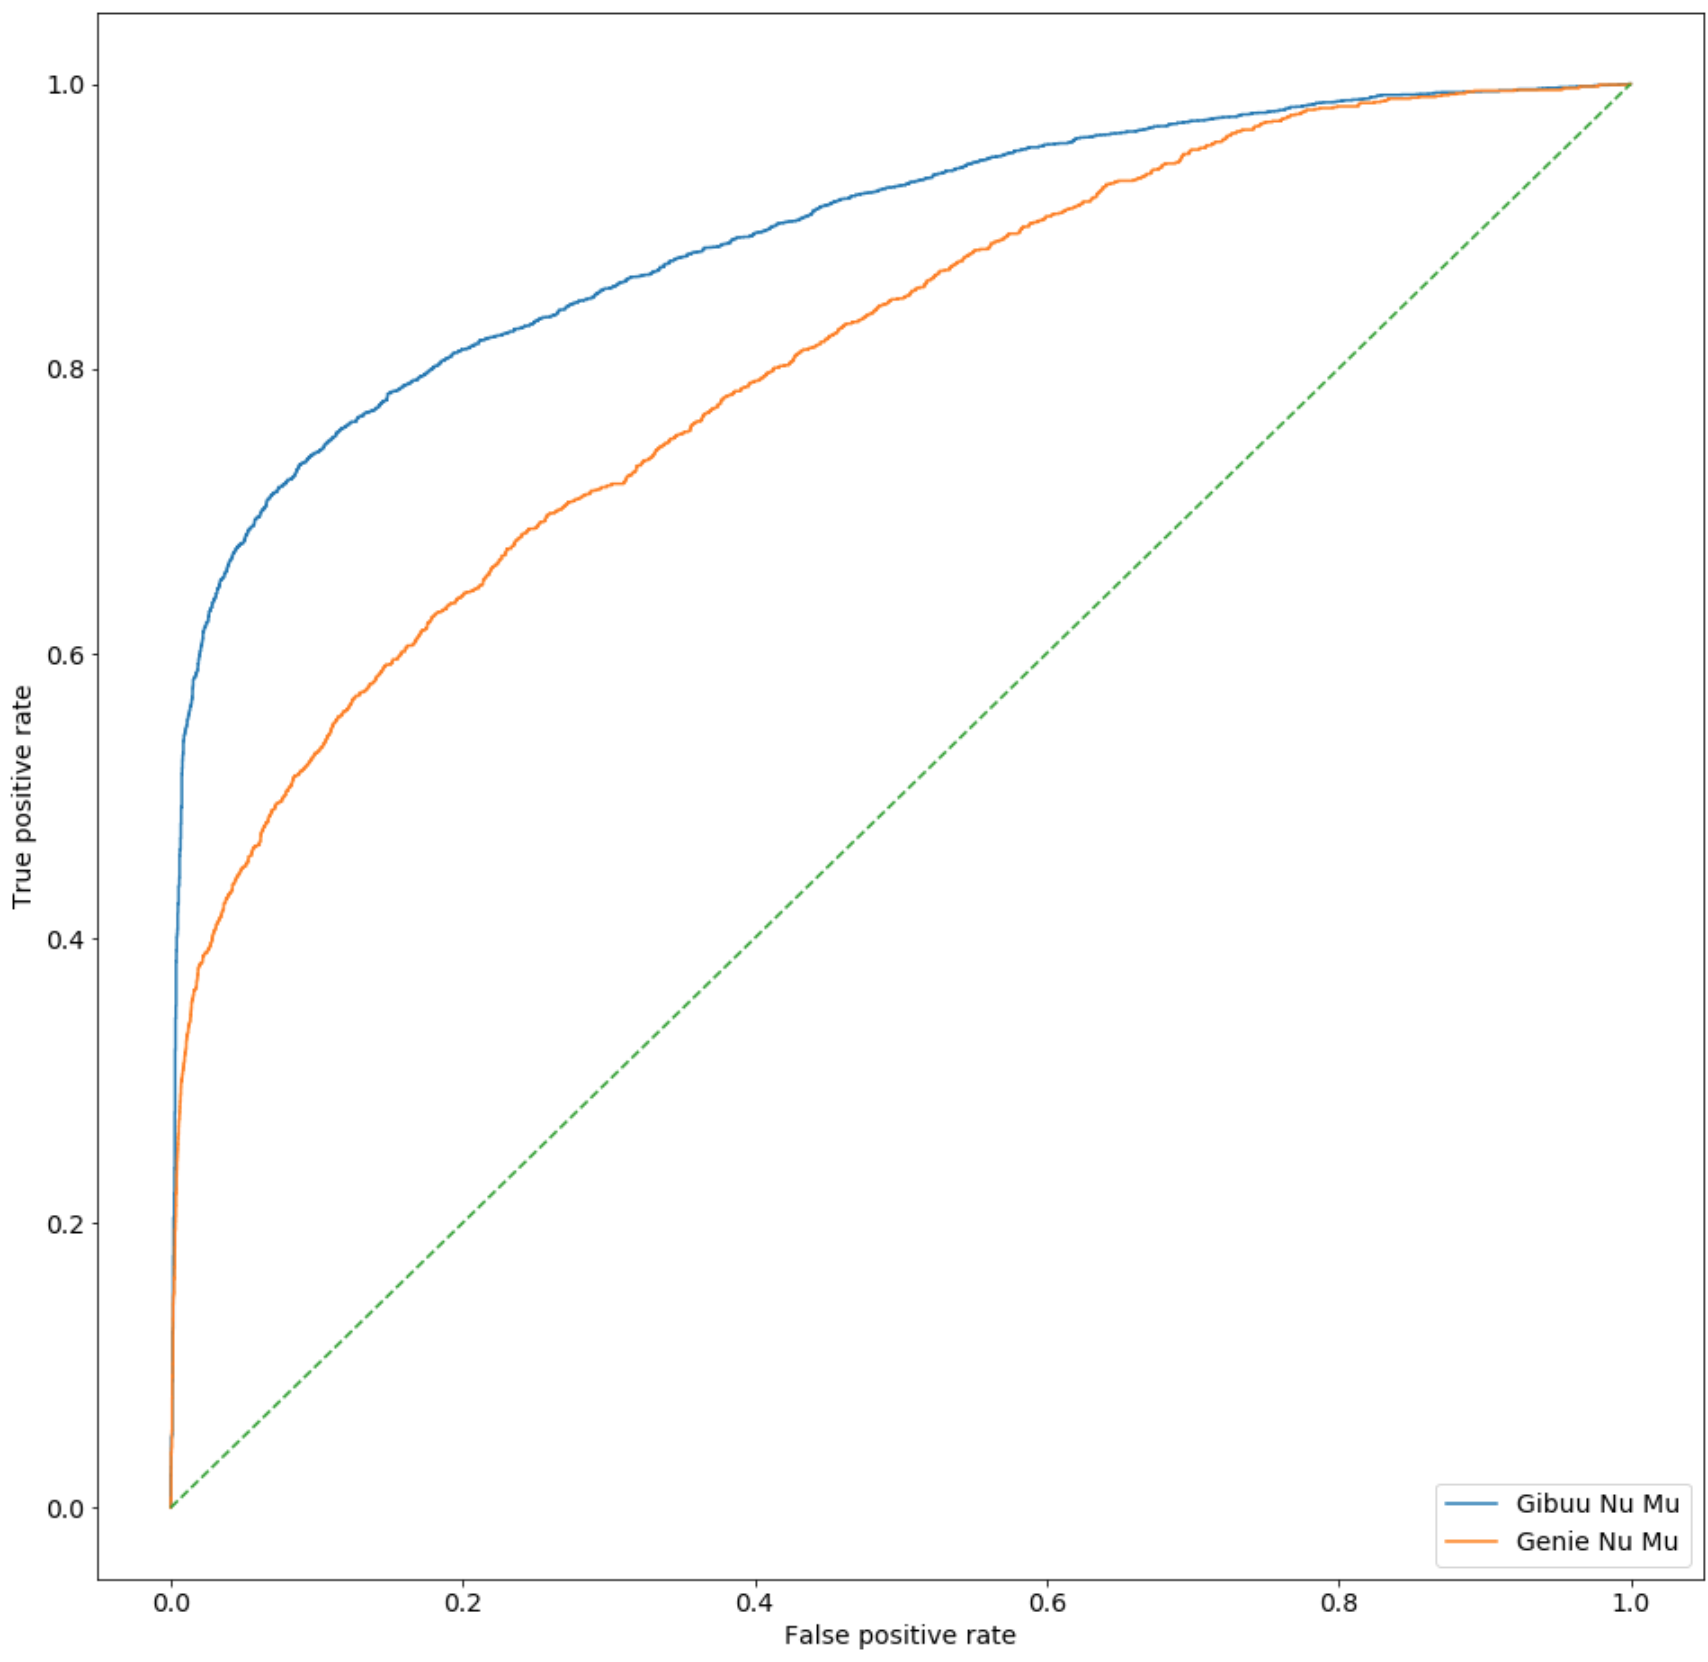
\includegraphics[width=75mm]{Both_Data/rocmu.png}
  \end{subfigure}
   \begin{subfigure}{}
 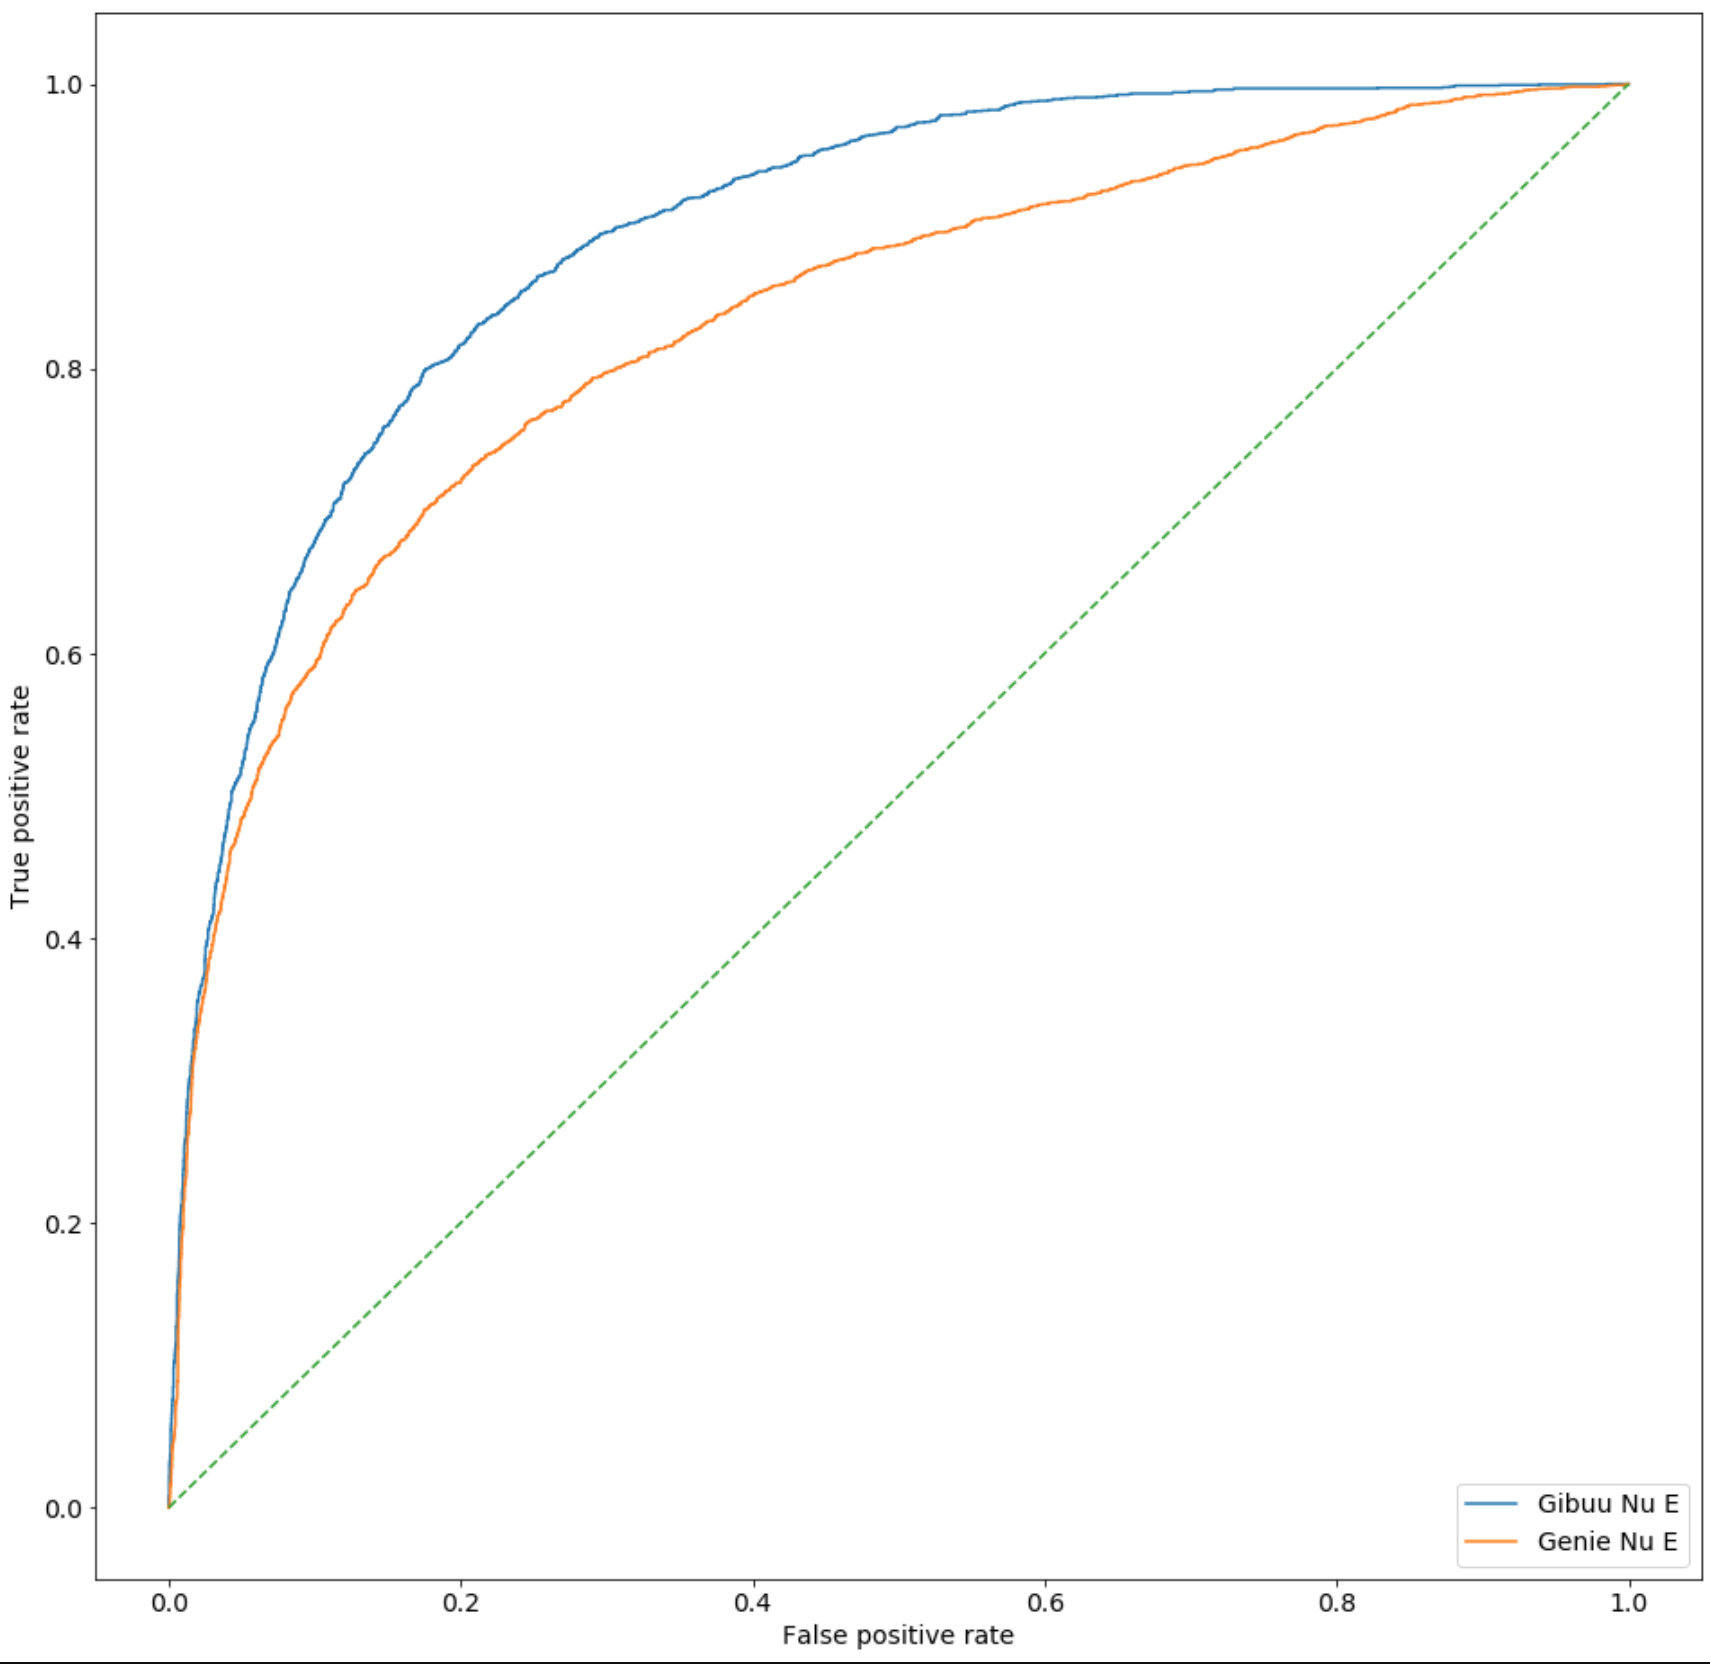
\includegraphics[width=75mm]{Both_Data/roce.png}
  \end{subfigure}
  
 \textbf{Figure 26.} \textit{ROC curves for $\nu_\mu$ classification on the left, and $\nu_e$ classification on the right. A blue curve represents GiBUU events and an orange curve, the GENIE events.}
\end{figure}

\noindent Using a Receiver Operating Characteristic (ROC) curve, which plots the true positive rate against the false positive rate of a binary classifier, in this case the classifier classifies whether the interaction was identified as a $\nu_\mu$ or not a $\nu_\mu$ event (and the same with the $\nu_e$ classifier to indicate how well the classifier performs, and provides a more intuitive visualisation for comparing performances. Figure 26 show the ROC curves for $\nu_\mu$ and the $\nu_e$ classifiers. The dotted line represents a random performance, and the closer a curve is to the upper left of the graph, the stronger the performance. By displaying the curves separately for GENIE and GiBUU events we are able to see that with both classifiers, the GiBUU events are classified with a higher accuracy than the GENIE events. This may be because a proportion of  GiBUU events are more distinctive in someway and the classifier learns how to classify these.\medskip







 

\subsection{Network Interpretability}

\noindent To try and understand why the network was classifying as it was, we decided to look at the node values of the penultimate layer of the trained network. This dense layer of 1024 nodes feeds into the final dense layer with 3 nodes, one for each of the classification types. By looking at the node activation layer, patterns emerge as to the importance of each node, and how the model has trained the weights and biases to learn how to classify each image for the result to be produced in the final output layer.\medskip

\begin{figure}[t!]
 \centering
 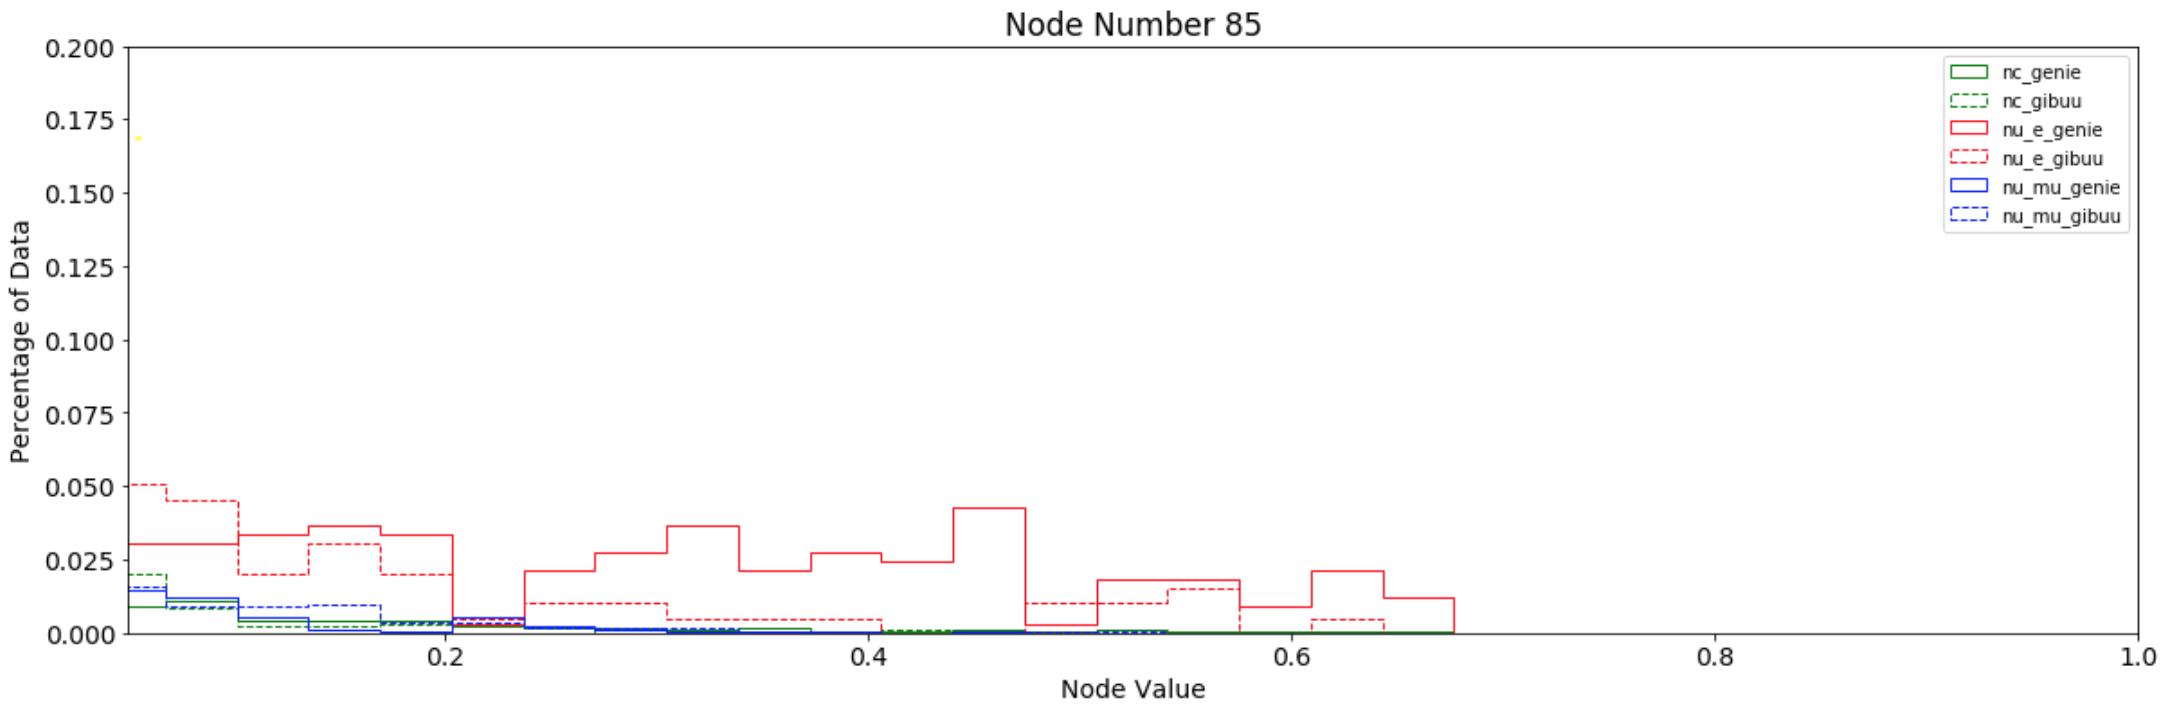
\includegraphics[width=160mm]{nodes/node01.png}
 
 \textbf{Figure 28.} \textit{Node activation values, for Node 85, for events of all three types and both event generators from the training process in section 3.1.4, where the network was trained and tested on equal GENIE and GiBUU combined data over 100 epochs.}

 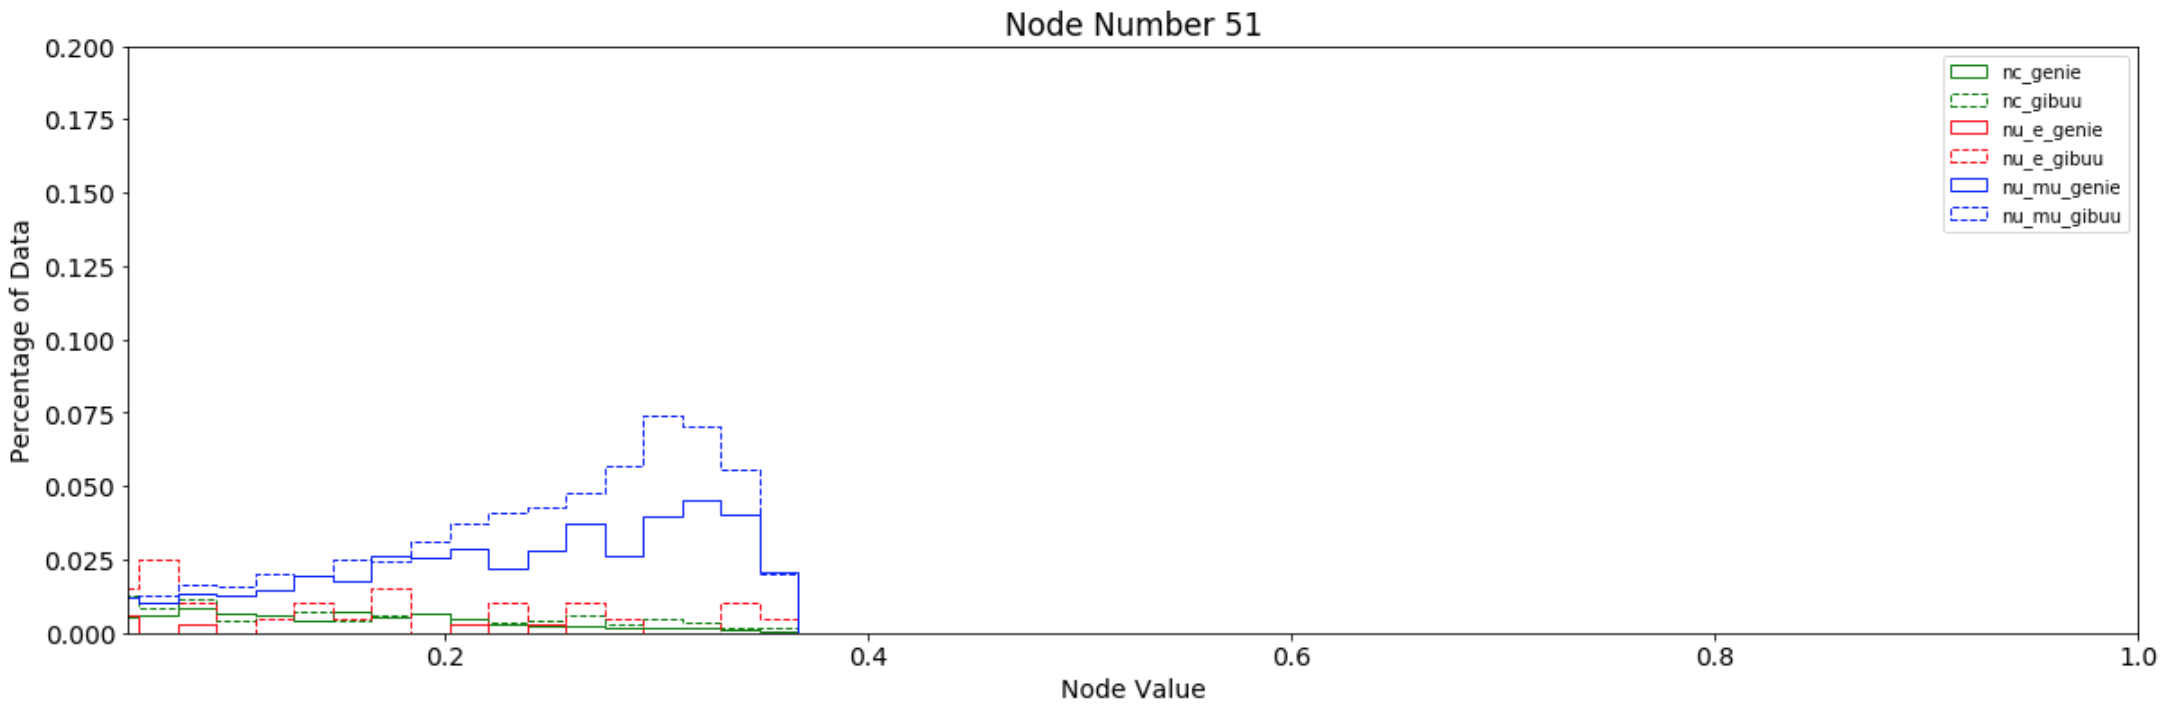
\includegraphics[width=160mm]{nodes/node02.png}
 
 \textbf{Figure 29.} \textit{Node activation values, for Node 51, for events of all three types and both event generators from the training process in section 3.1.4.}

 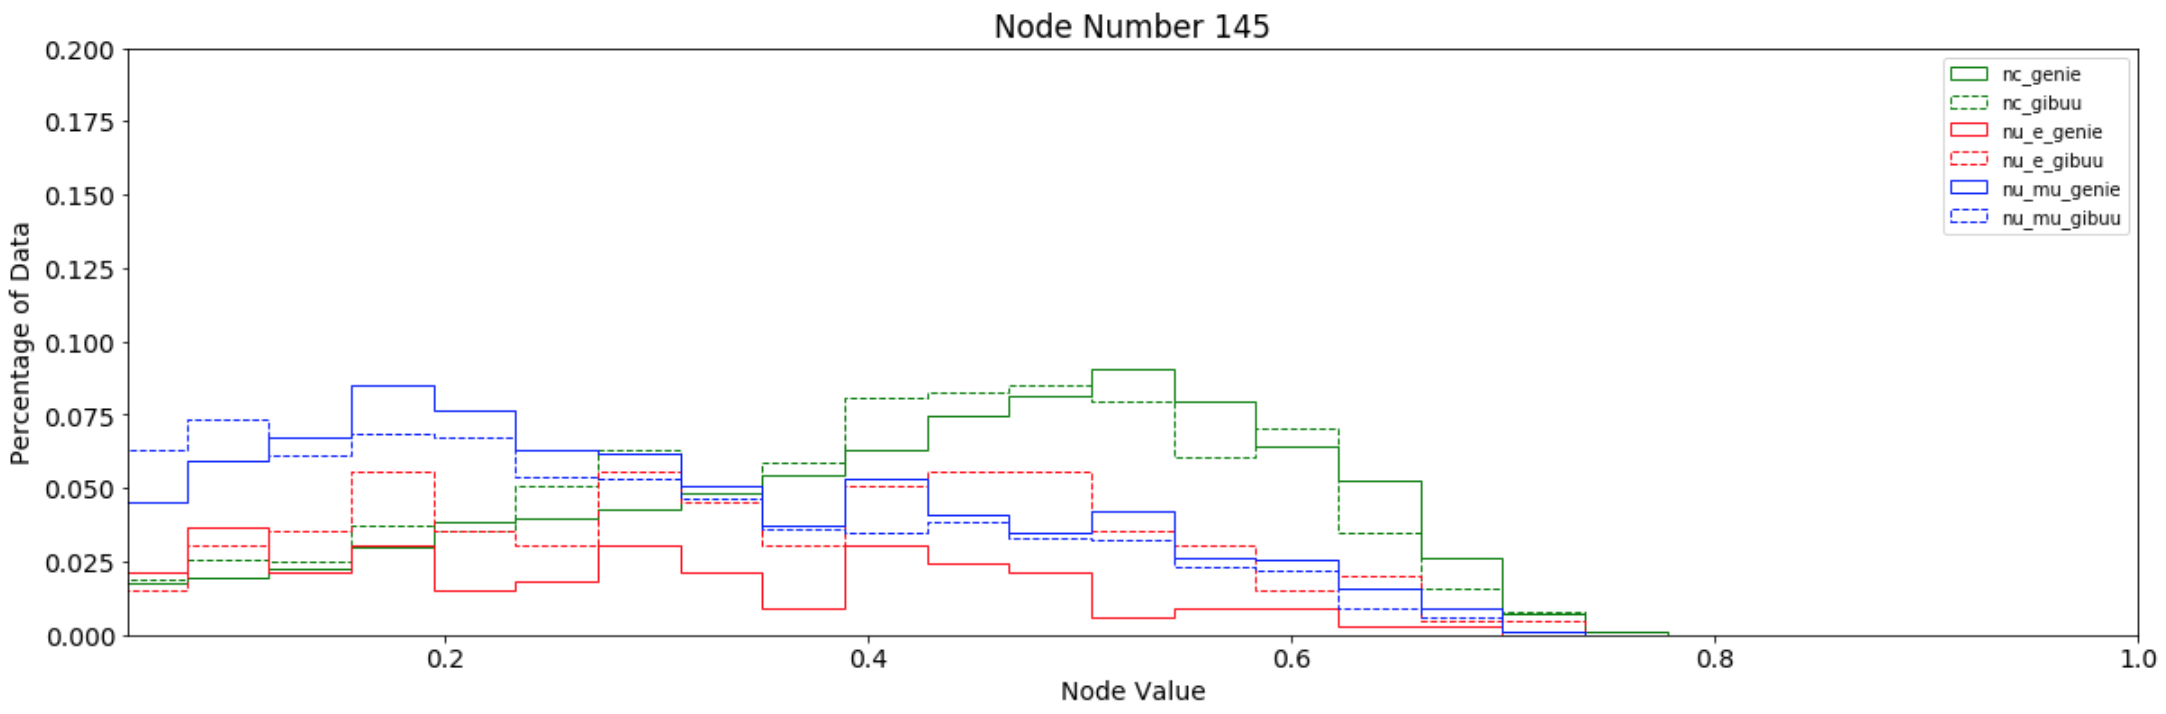
\includegraphics[width=160mm]{nodes/node03.png}
 
 \textbf{Figure 30.} \textit{Node activation values, for Node 145, for events of all three types and both event generators from the training process in section 3.1.4.}
\end{figure}



\noindent This analysis was performed on the classifier trained in section 3.1.4, which contained an equal number of events of each of the interaction type and from GENIE and GiBUU. The majority of the nodes in the final layer, 78.4\%, did not activate for any of the events and as a result would have no impact on the final classification. By plotting a histogram of the values of the nodes, and separating the distributions depending on interaction type and generator source, it became clear that activation of certain nodes indicates how the model will classify the event. An example was node 85, see Figure 28, here it can be seen that, on the most part, if the node is activated, the event will be classified as a $\nu_e$ event, especially at large values. This is also visible in Figure 29, where activation mostly indicates that the event will be classified as a $\nu_\mu$ event, and this is more apparent at large values of the node.\medskip

\noindent With some nodes, see Figure 20, certain values of the node indicate the classification of the event, with overlapping regions of the distributions visible. While many indicate the domain source of the event. This can be seen in Figure 31, where the largest values of the node activation are produced when the event is a GiBUU produced $\nu_\mu$ event. In Figure 32, the largest activation values occur when a GENIE produced $\nu_e$ event is passed through the network for classification.\medskip

\begin{figure}[t!]
 \centering
 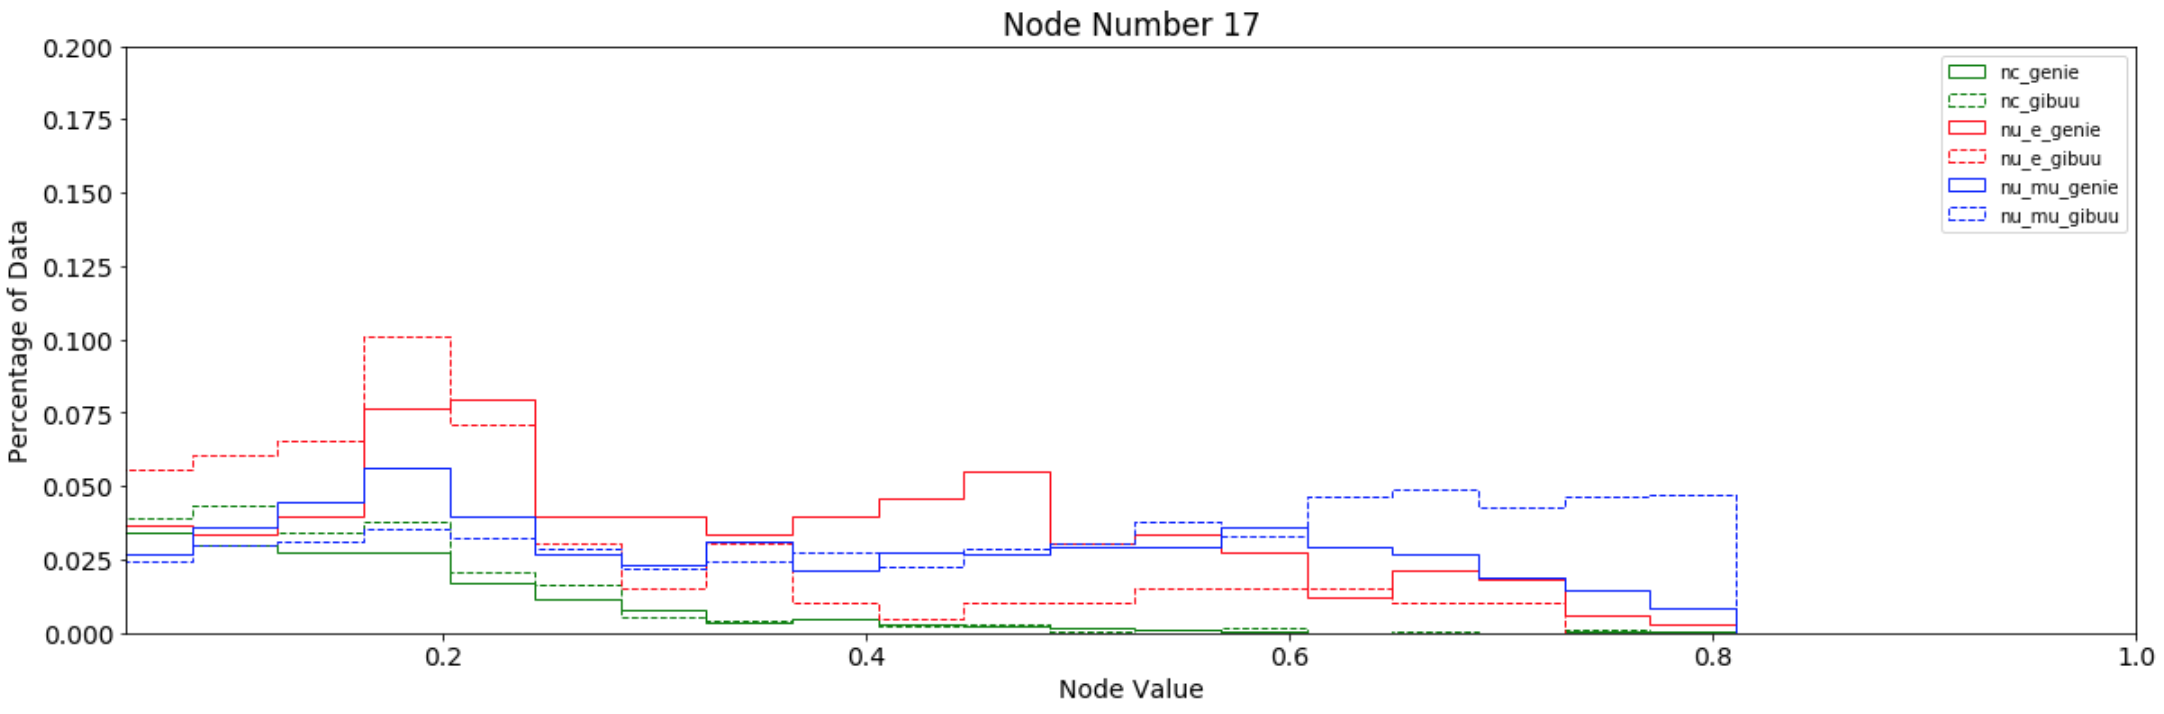
\includegraphics[width=160mm]{nodes/node04.png}
 
 \textbf{Figure 31.} \textit{Node activation values, for Node 17, for events of all three types and both event generators from the training process in section 3.1.4.}

 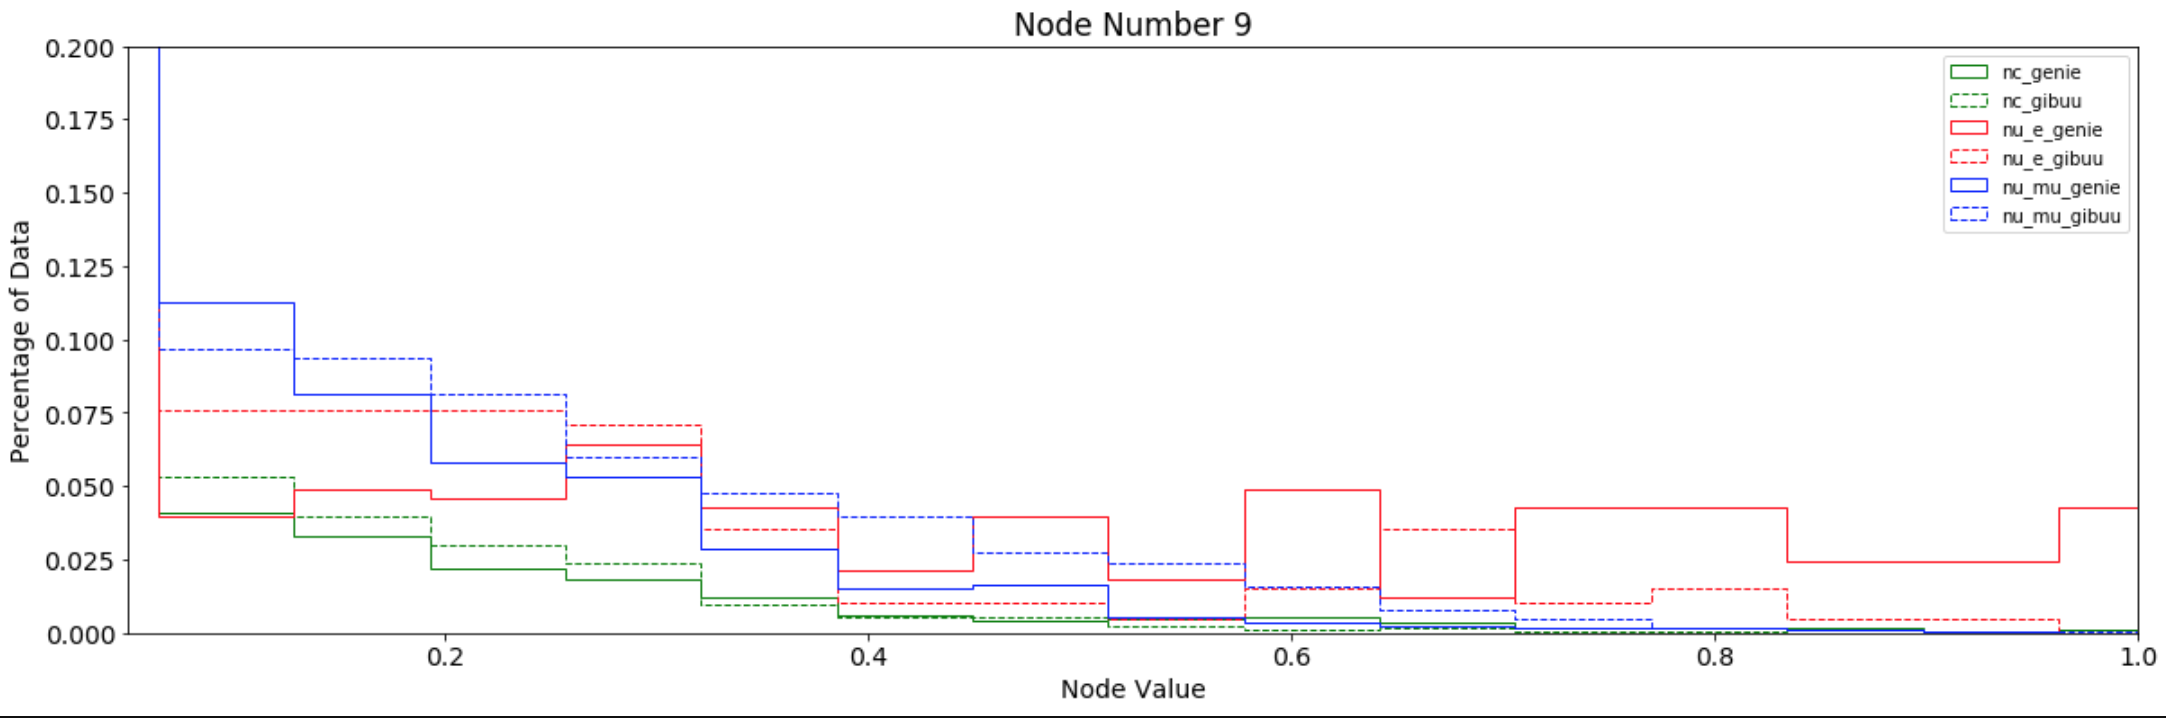
\includegraphics[width=160mm]{nodes/node05.png}
 
 \textbf{Figure 32.} \textit{Node activation values, for Node 9, for events of all three types and both event generators from the training process in section 3.1.4.}
\end{figure}

\noindent In order to be able to determine any patterns over the entirety of the penultimate node layer, rather than using qualitative methods on an individual basis, the node activation values were treated as distributions, for the various event types. Here the event types consisted of the 3 event interaction types and the two event generators. The maximum value of the purity efficiency functions was taken to represent each interaction type for each node. For each interaction type, ie. GENIE generated or $\nu_\mu$, an array was produced for the maximum purity efficiency values for each node. In order to see if there were any correlations between the values for each interaction type the arrays were plotted against each other as scatter plots.\medskip

\noindent While this may not be the most robust operation, what it does enable it the quantification of the separation of these node value distributions. By treating the node histograms as distributions, a purity efficiency curve will determine the separation of that distribution, from the background- the other event types. As significant patterns are being looked for in the higher values of nodes, as these are where greater activation has taken place, a purity efficiency calculation is appropriate, as these methods are used for classifications where correct classification is given by greater activation at higher confidence levels.\medskip

\begin{figure}[h]
 \centering
 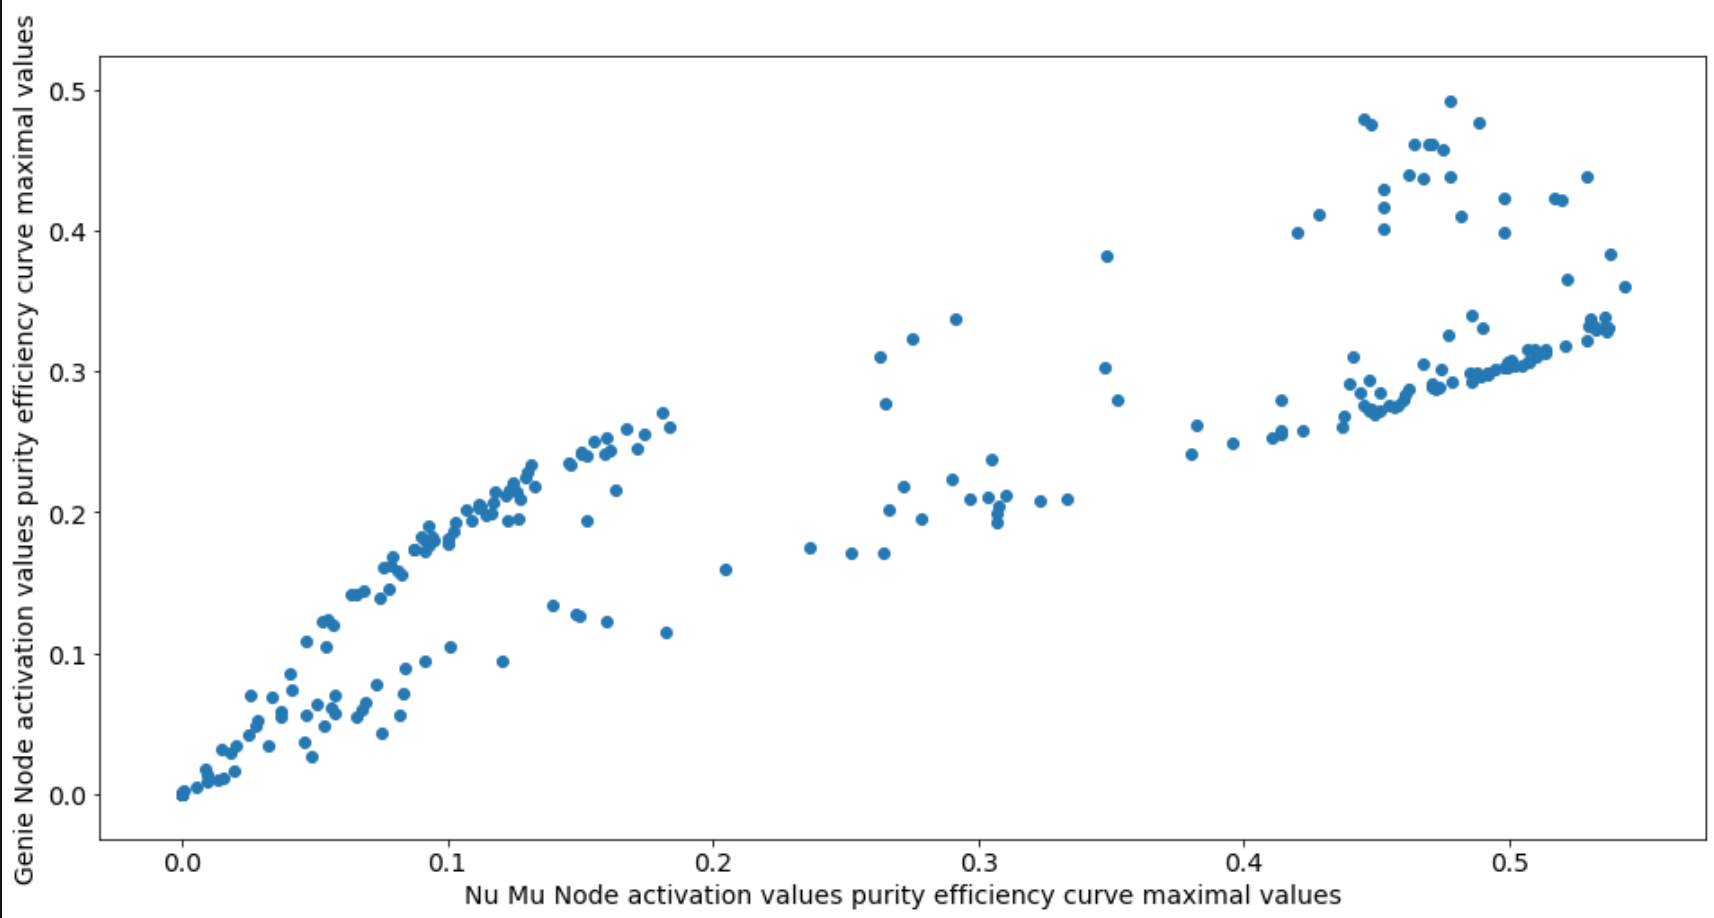
\includegraphics[width=100mm]{nodes/nodes2.png}
 
 \textbf{Figure 33.} \textit{Node activation values purity efficiency curve maximal values over all nodes to see the correlation between $\nu_\mu$ events and GibUU generated events}

\end{figure}

\noindent Most combinations showed no correlation, however the strongest correlation can be seen between the $\nu_\mu$ events and the GibUU events. This indicates that node activation where there was a measured separation were able to measure such for certain nodes for both $\nu_\mu$ events and GibUU events. An example of this would be Figure 33, where the largest activation was seen by GibUU produced $\nu_\mu$ event. The strong positive correlation indicates that there is a correlation between how easily the classifier classified the event, and if that event was a $\nu_\mu$ produced by GibUU produced, meaning these events have features that make them easily identifiable, or have features that were well learned by the model.\medskip



 
\newpage

\section{Domain Classification}

\begin{figure}[h]
 \centering
 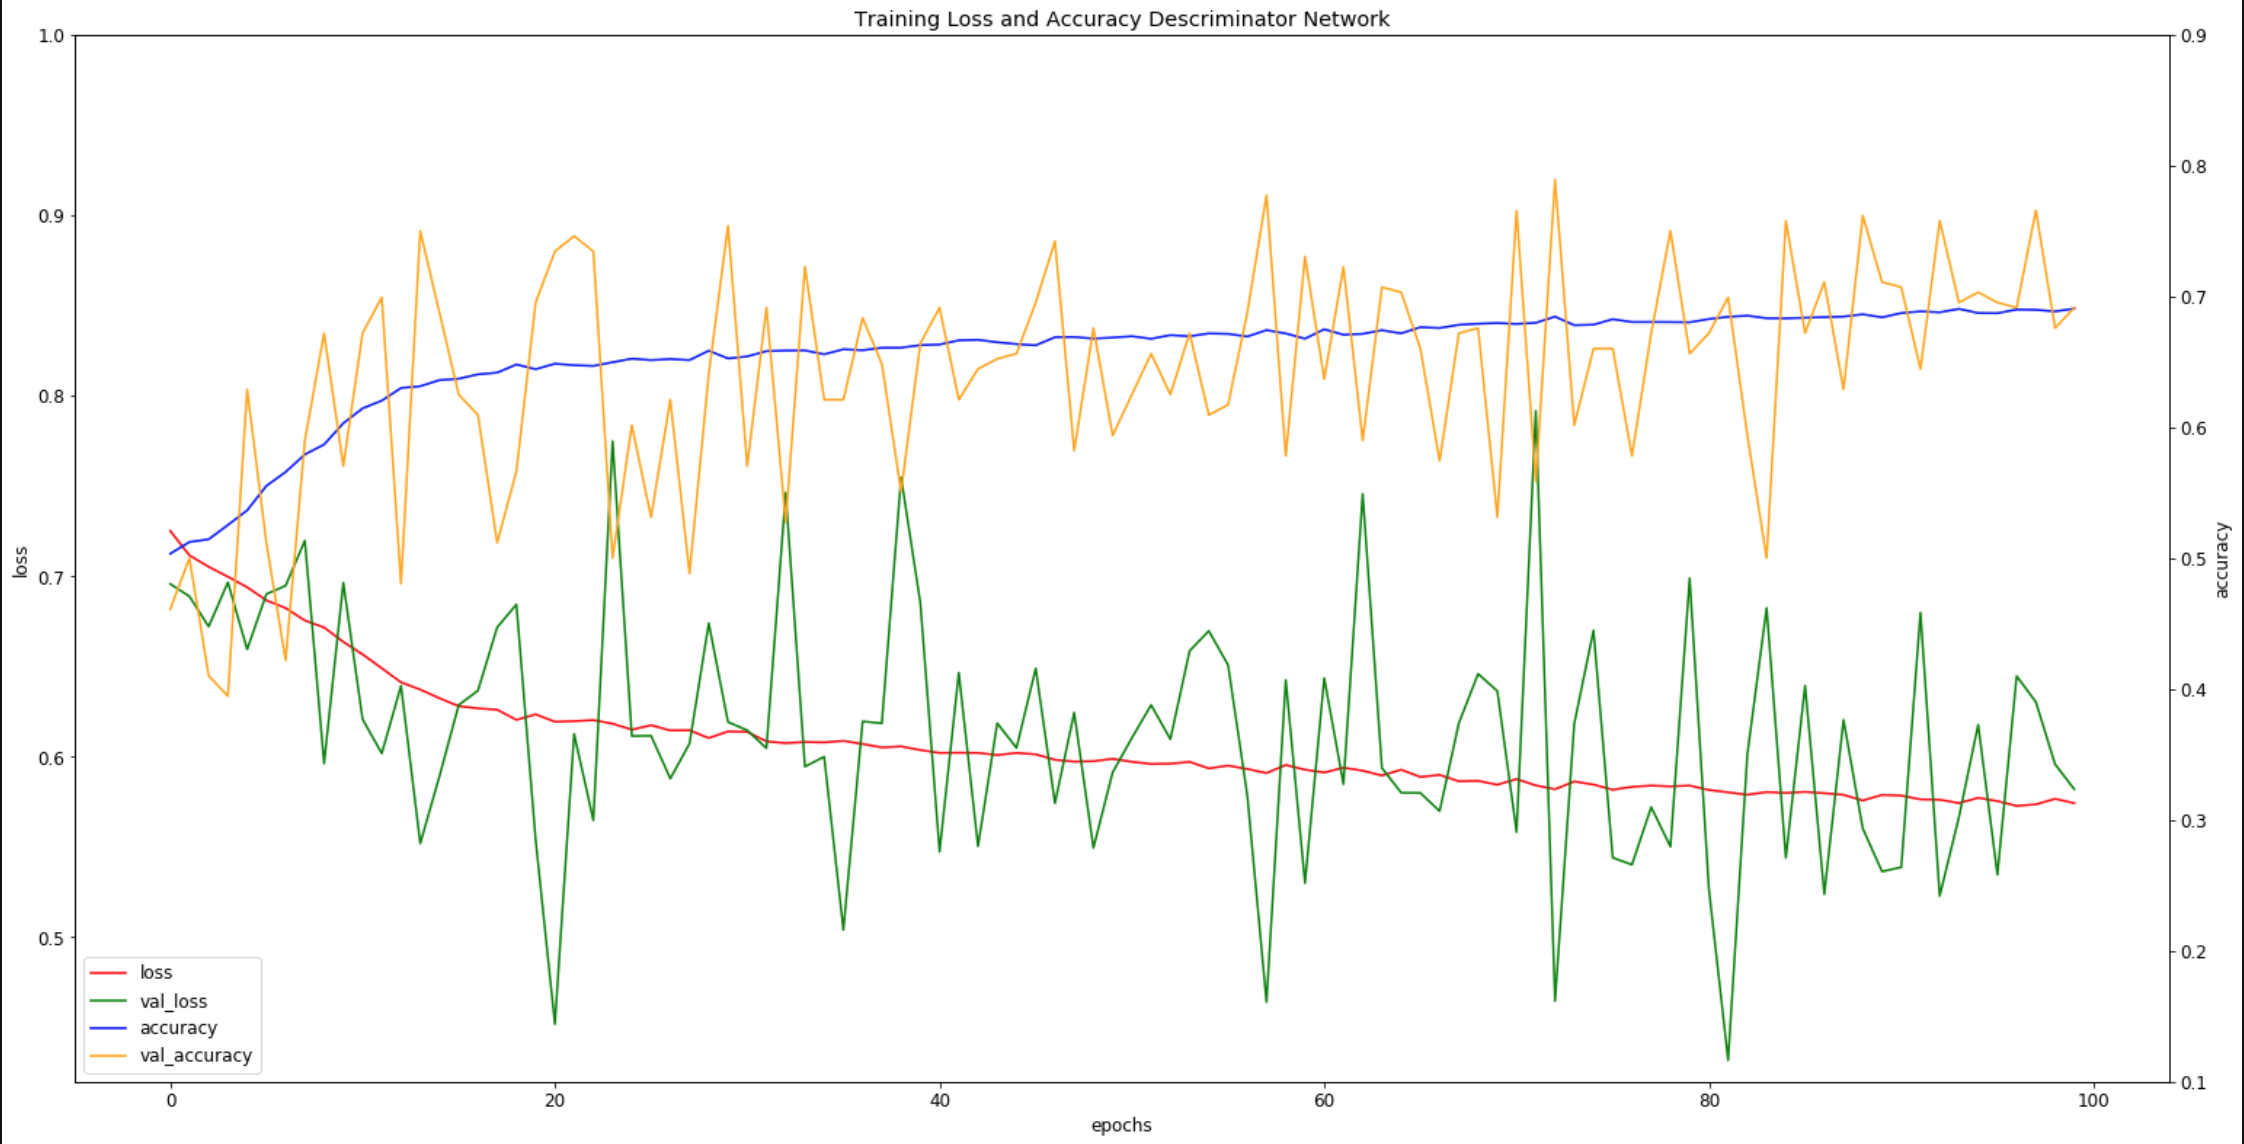
\includegraphics[width=160mm]{Descr/train.png}
 
  \textbf{Figure 34.} \textit{Network training and validation accuracy and loss for a discriminator network. The network was trained over 100 epochs using both GENIE and GENIE generated events. With an equal number of all three event types.}
\end{figure}

\begin{figure}[t!]
 \centering
 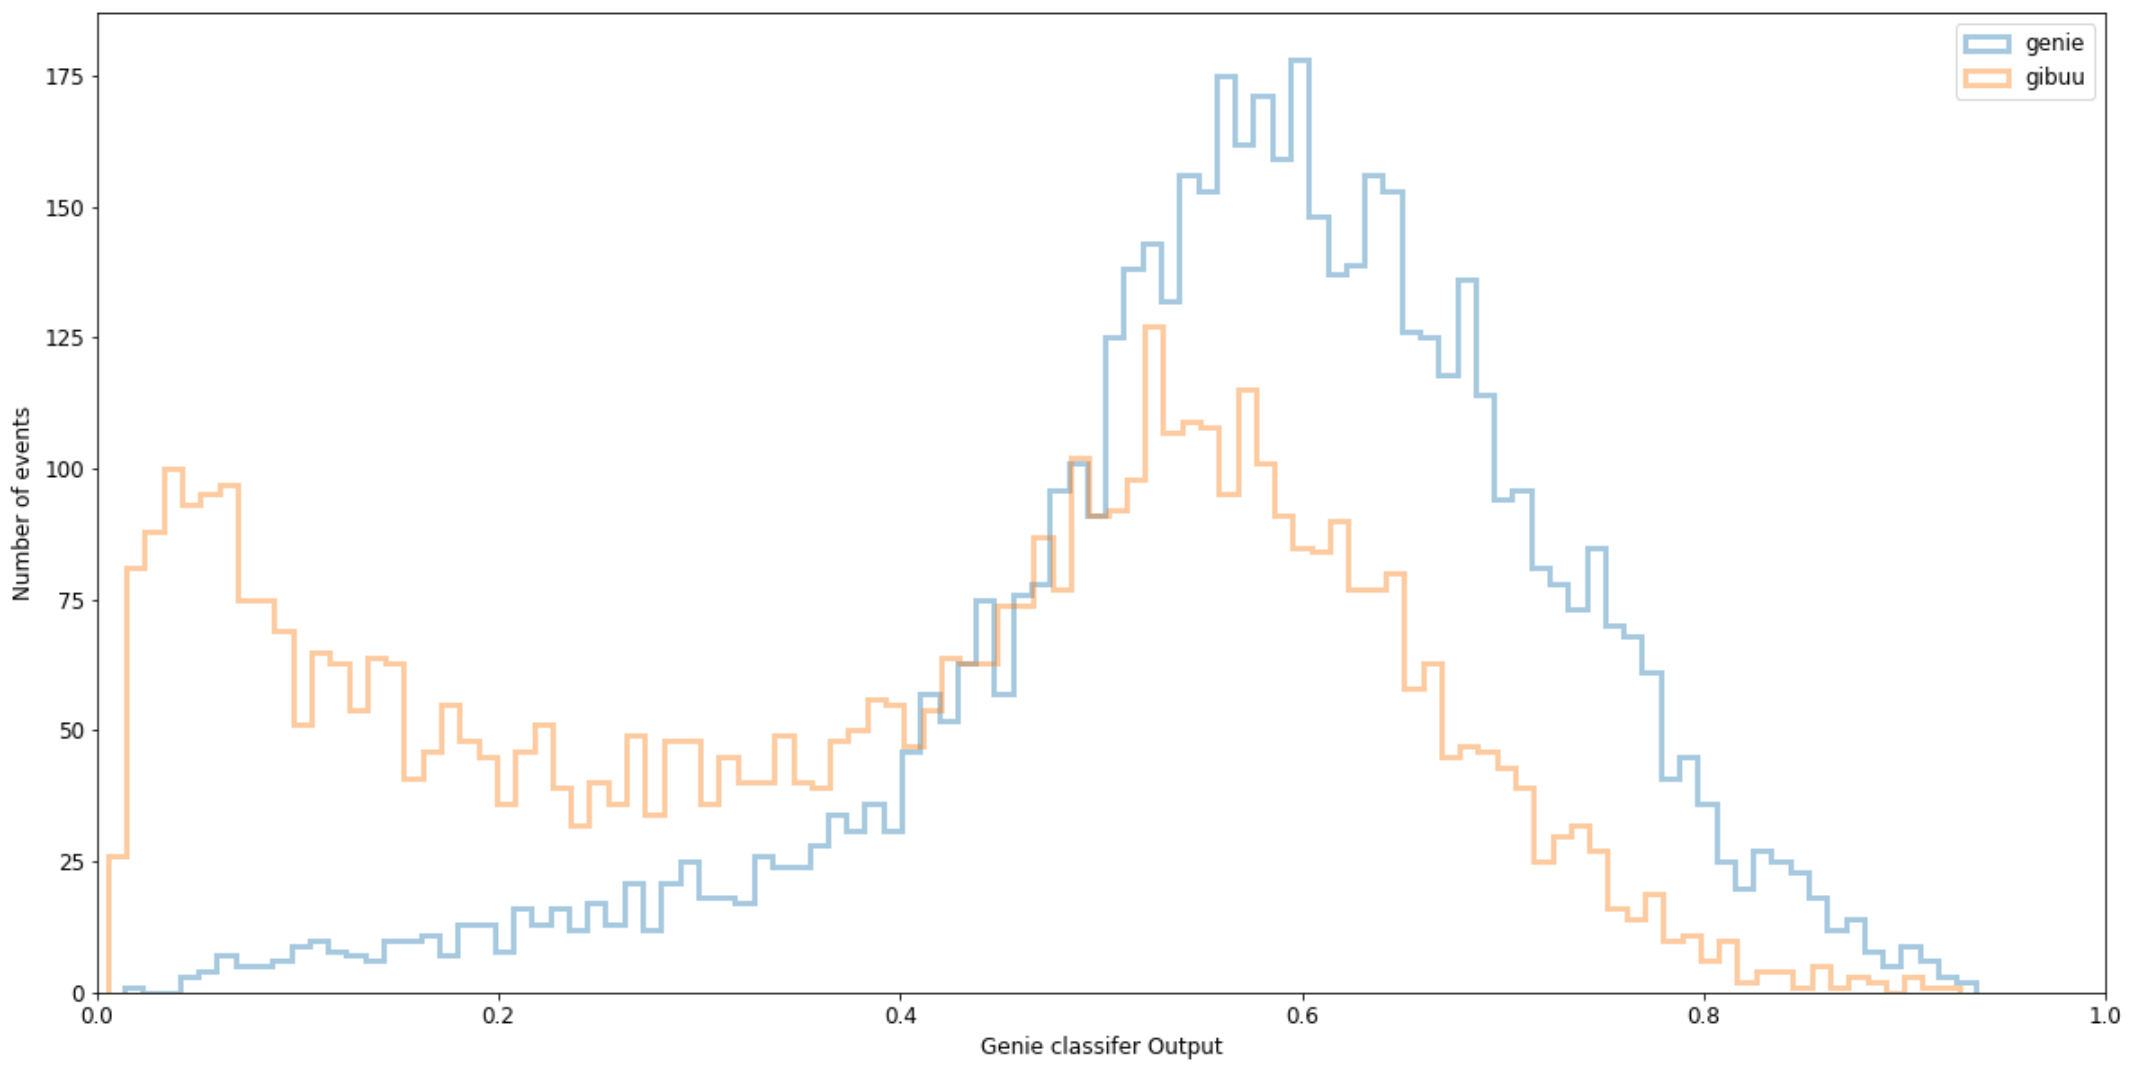
\includegraphics[width=160mm]{Descr/class.png}
 \textbf{Figure 35.} \textit{GENIE event classification output histogram. The dataset was trained and tested using an equal number of GENIE and GiBUU generated events. The dataset contained an equal number of the interaction types.}
\end{figure}

\begin{figure}[t!]
 \centering
 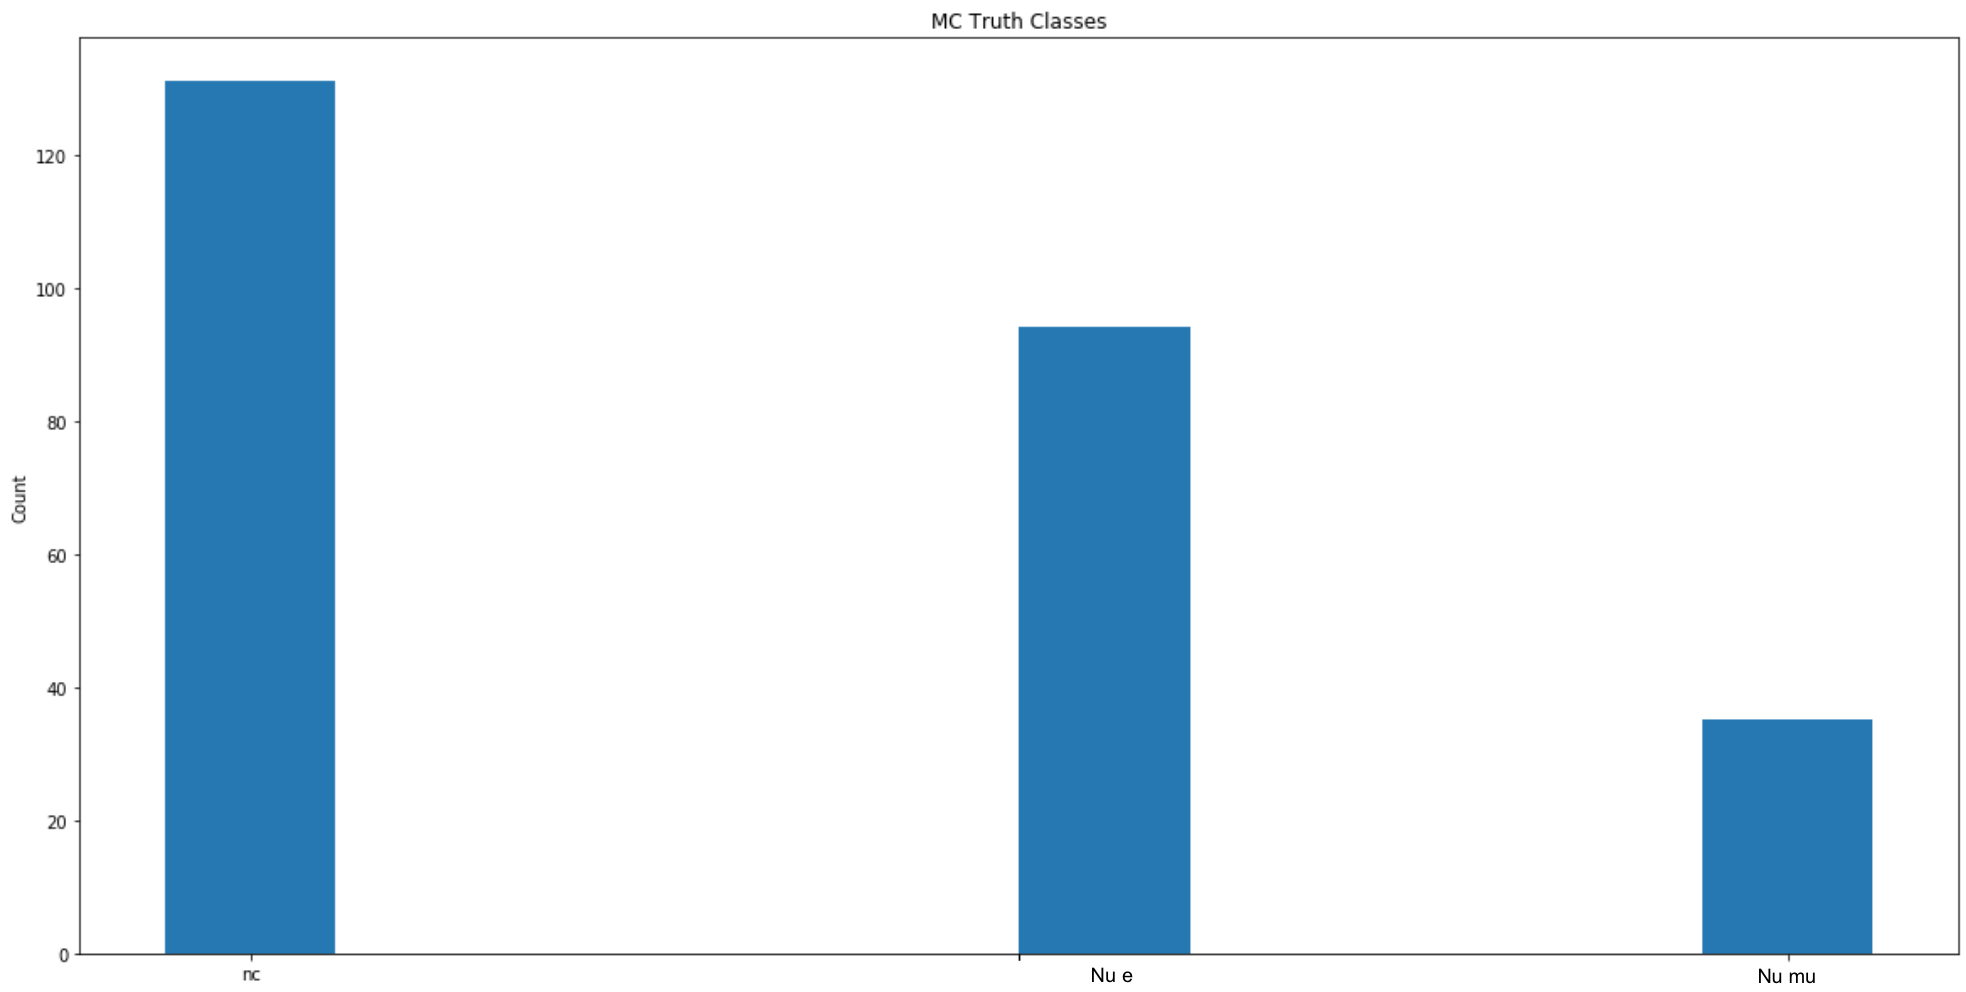
\includegraphics[width=160mm]{Descr/int.png}
 \textbf{Figure 36.} \textit{Histogram of the interaction types of events that the discriminator correctly identified as GiBUU events, with a confidence of greater tha 70\%}
\end{figure}


\noindent The network was modified to classify the events according to their production domain. In the training there were an equal number of GENIE and GiBUU events, as well as an equal number of each interaction type, to ensure that the model could train fairly and was not influenced by the distribution of events that may or may not be indicative of the domain. In Figure 34, the model does not appear to overfit, and the increase in accuracy tends to zero very quickly within the 100 epoch training process. The classification distribution can be seen in Figure 35 where there GENIE classifier output can be seen. The GiBUU classifier output is not shown as this is a binary classification task, and the GiBUU classifier is identical to that of the GENIE classifier simply reflected about the y-axis. \medskip

\noindent From Figure 35 we can see that the network struggles to classify the events from the two domains with confidence. Majority of the GENIE events are correctly classified with a probability between 50\% and 75\%. However with a very similar probability distribution a large proportion of the GiBUU events are incorrectly classified as GENIE events, indicating that these events are similar in appearance. However, with a confidence of 80\% and above (20\% and below on the GENIE classifier) the classifier correctly identifies a number of GibUU events, indicating that these events are fundamentally different in nature to the other GiBUU events, as well as the GENIE events that were incorrectly predicted as not GENIE events with a confidence of 80\%, and it is this difference in production nature that may cause bias in the interaction type classification when classifying events from the two different domains.\medskip

\noindent Figure 36 shows the interaction type of the events that are strongly classified as GiBUU events. There is a spread in the event types rather than one event type in particular being produced differently by GENIE and GiBUU. The $\nu_\mu$ feature the least here and one would expect this is because of the nature of $\nu_\mu$ interaction where the resultant $\mu$ leaves a very definite track. This may also explain why the classifier in section 3.1.4 was much more confident in correctly predicting the $\nu_\mu$ events- because they are easier to distinguish, as well as there being less variation between how the events are simulated between GENIE and GiBUU. \medskip

To try and understand the physical properties of these events, in Figure 37 the number of hits value is plotted for the GiBUU events that were classified as definitely GiBUU events, with a GENIE output value of less than 0.2, the GENIE events of the same GENIE output value and the GiBUU events with a GENIE classification output value of greater than 0.3. What can be seen is that the GiBUU events that were easily distinguishable are unique in their physical properties. They, on average, produce a much larger number of hits, than any other event, and in Figure 38 are seen to have much larger sum of FLS hits that made CellHits from this neutrino, energy values- unlike the rest of the events that typically have very low energy values here. The large number of hits suggests that these events have large showers- it then makes sense that they are mostly comprised of $\Nu_e$ events and $NC$ that look very similar.


\begin{figure}[t!]
 \centering
 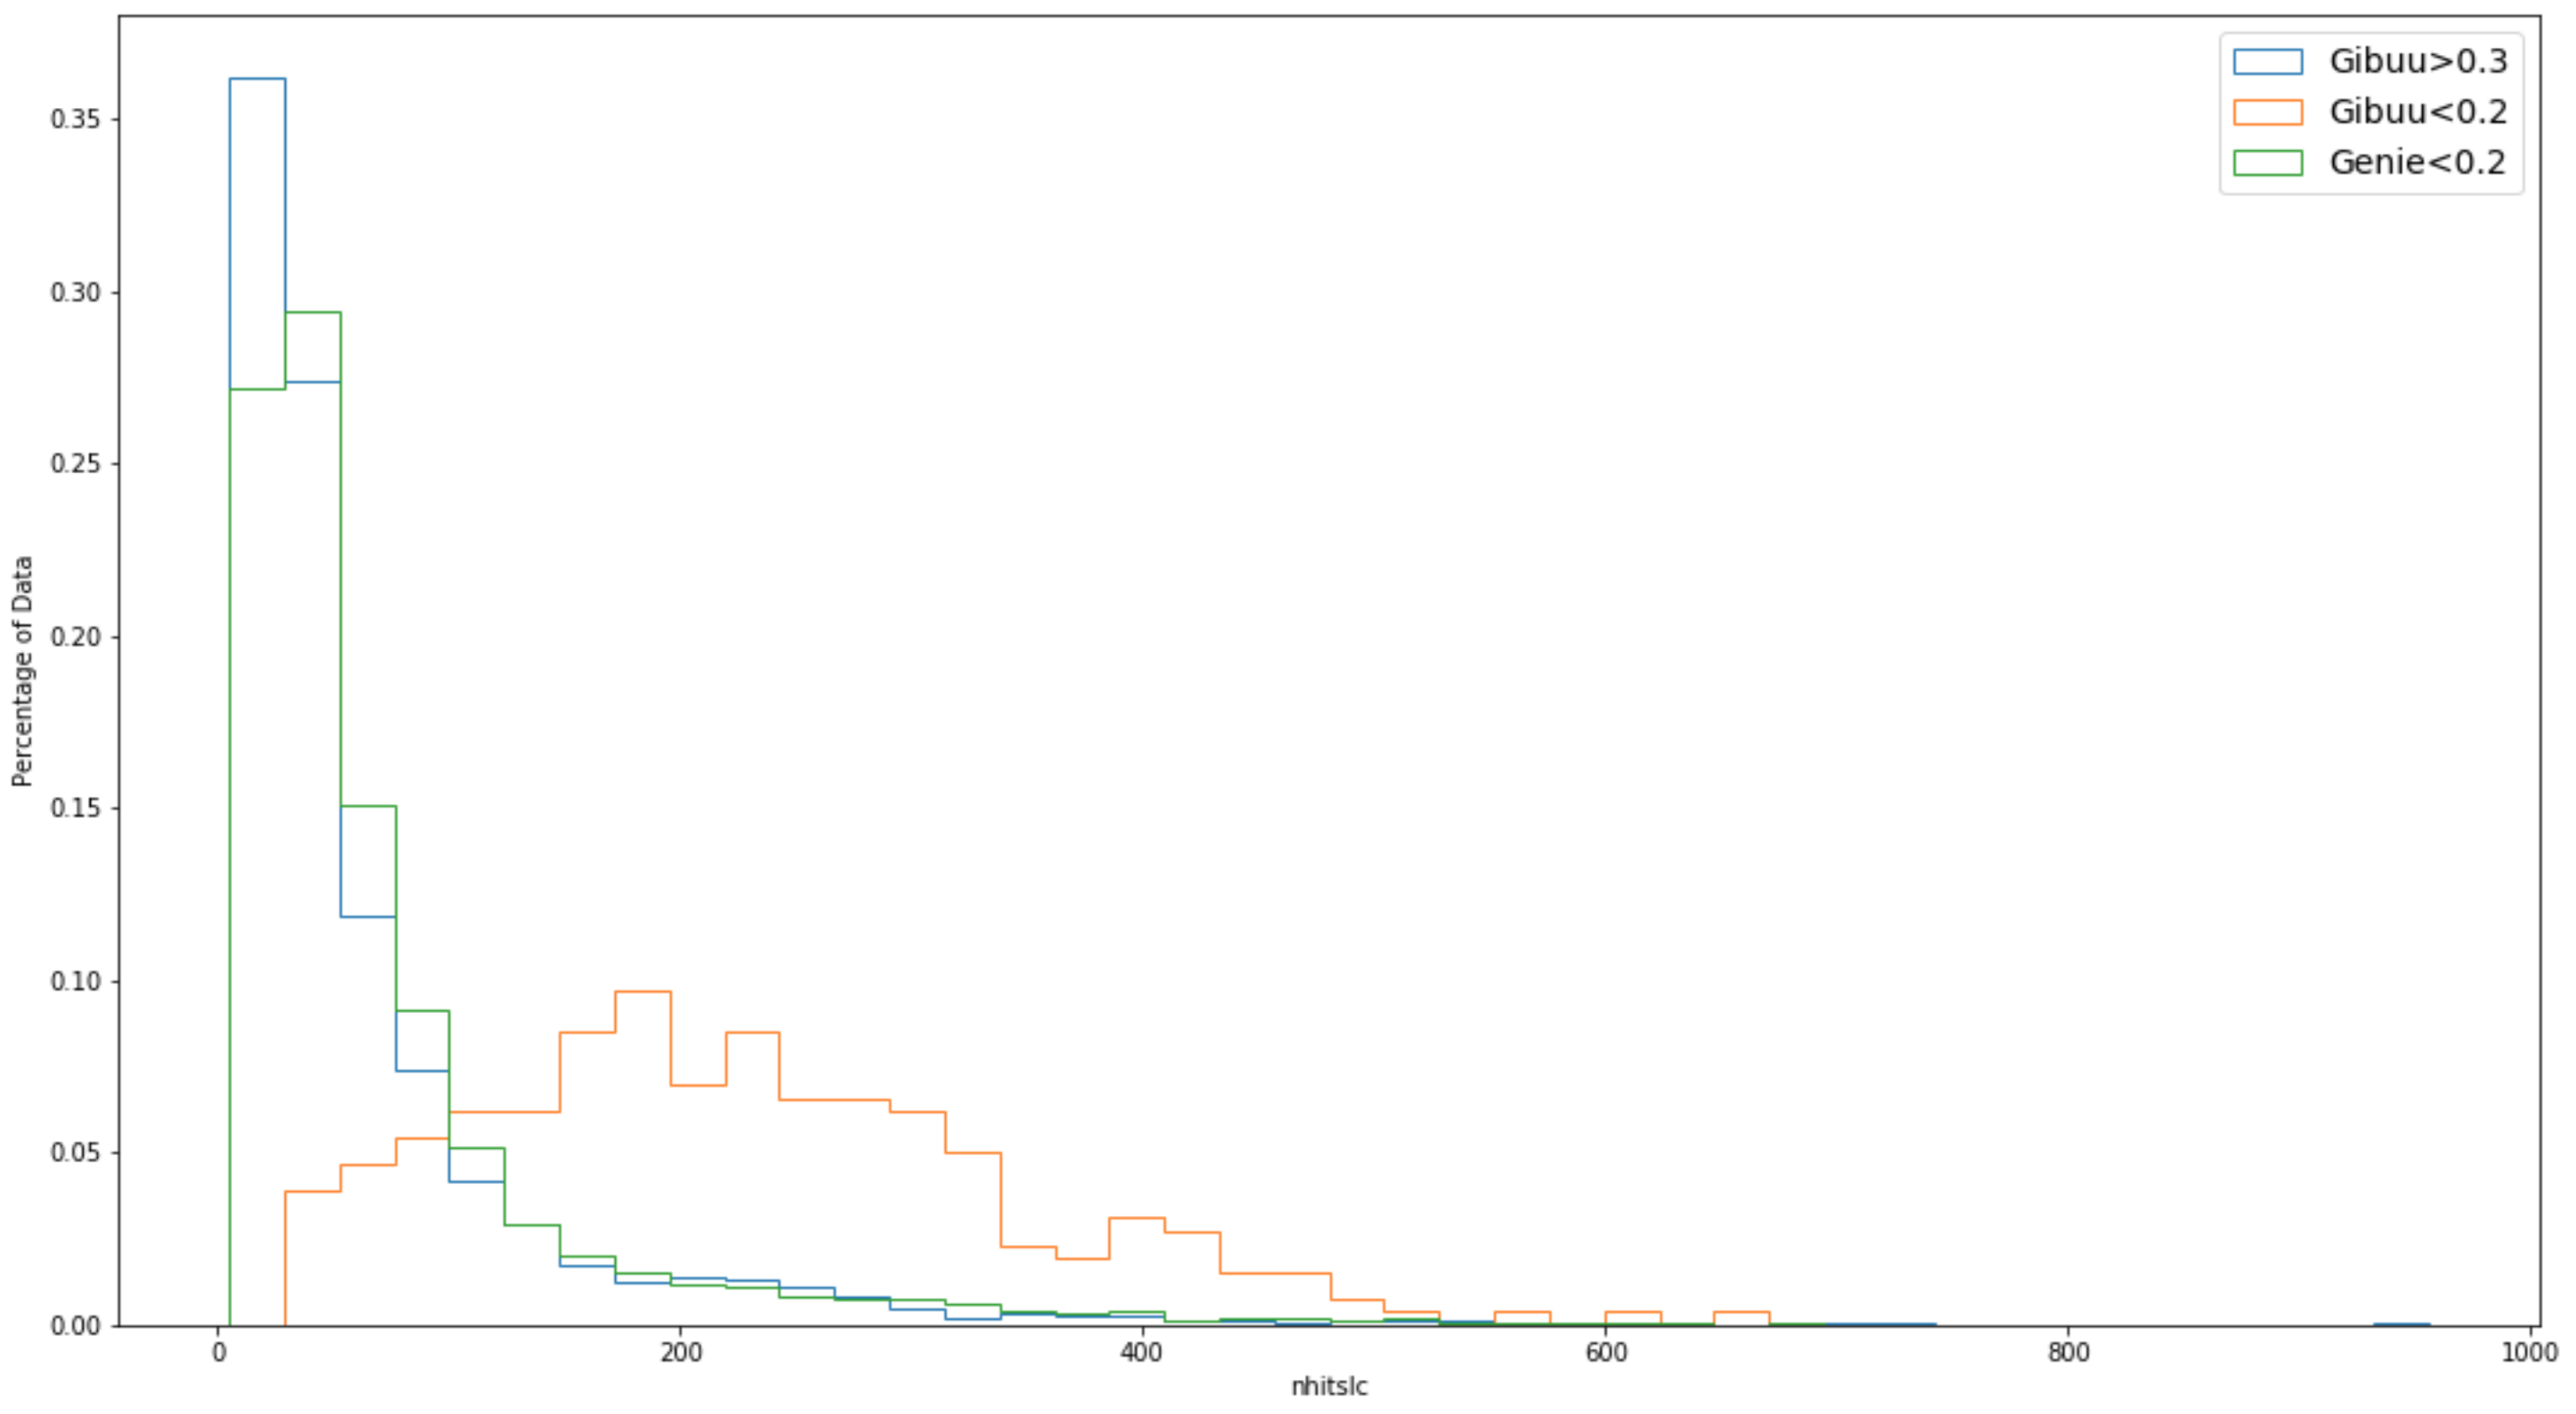
\includegraphics[width=160mm]{Descr/nhits.png}
 \textbf{Figure 37.} \textit{nhitslc- number of hits value plotted for events that with GENIE classification values of less that 20\% for both GENIE and GiBUU events, and greater than 30\% for GiBUU events, from the discriminator network}
\end{figure}

\begin{figure}[t!]
 \centering
 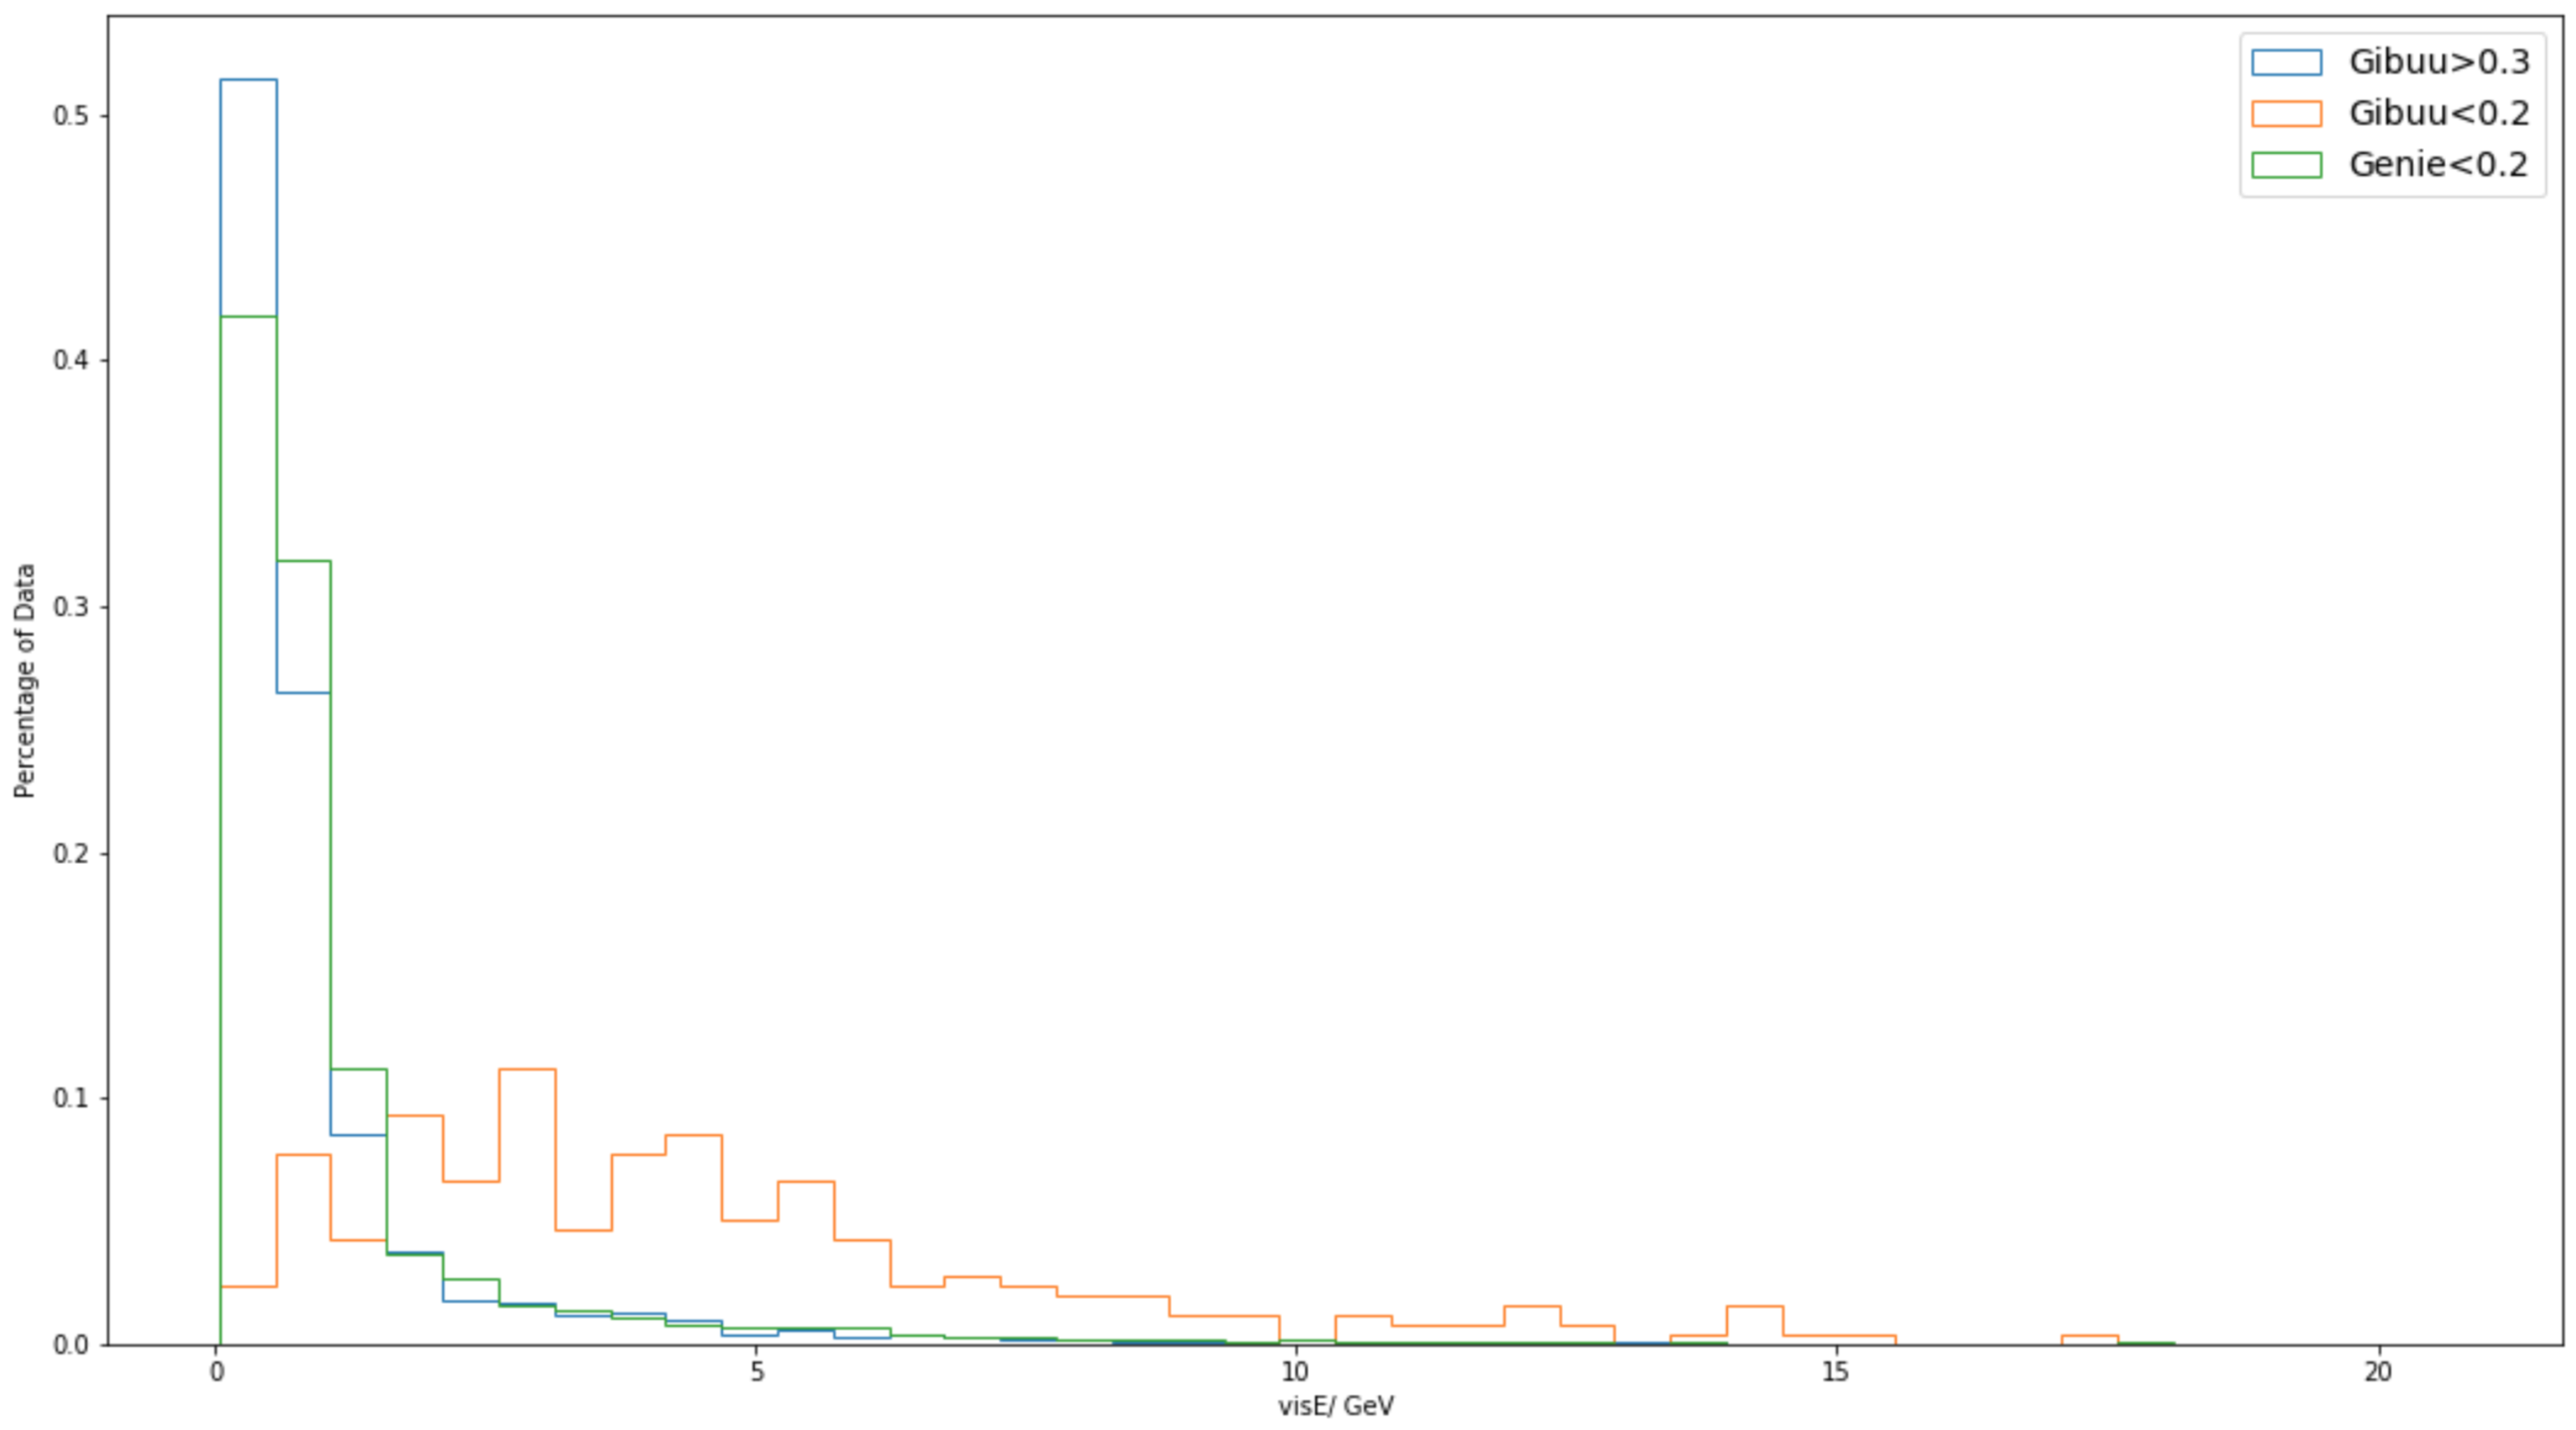
\includegraphics[width=160mm]{Descr/visE.png}
 \textbf{Figure 38.} \textit{visE- sum of FLS hits that made CellHits from this neutrino, energy value value plotted for events that with GENIE classification values of less that 20\% for both GENIE and GiBUU events, and greater than 30\% for GiBUU events, from the discriminator network}
\end{figure}

\newpage
 
\newpage
\section{Domain Adversarial Training}

\noindent The approach to see if a classifier that was invariant to these domain variations was to train a DANN that appended the CNN model that had been used previously. In order to determine the effectiveness of the DANN in producing a robust network invariant to the domain that the event was produced by, the feature classifier network was measured in the same way that the classifier networks were, and the purity efficiency curves were used to  determine the performance of the network.\medskip

\begin{figure}[t!]
 \centering
 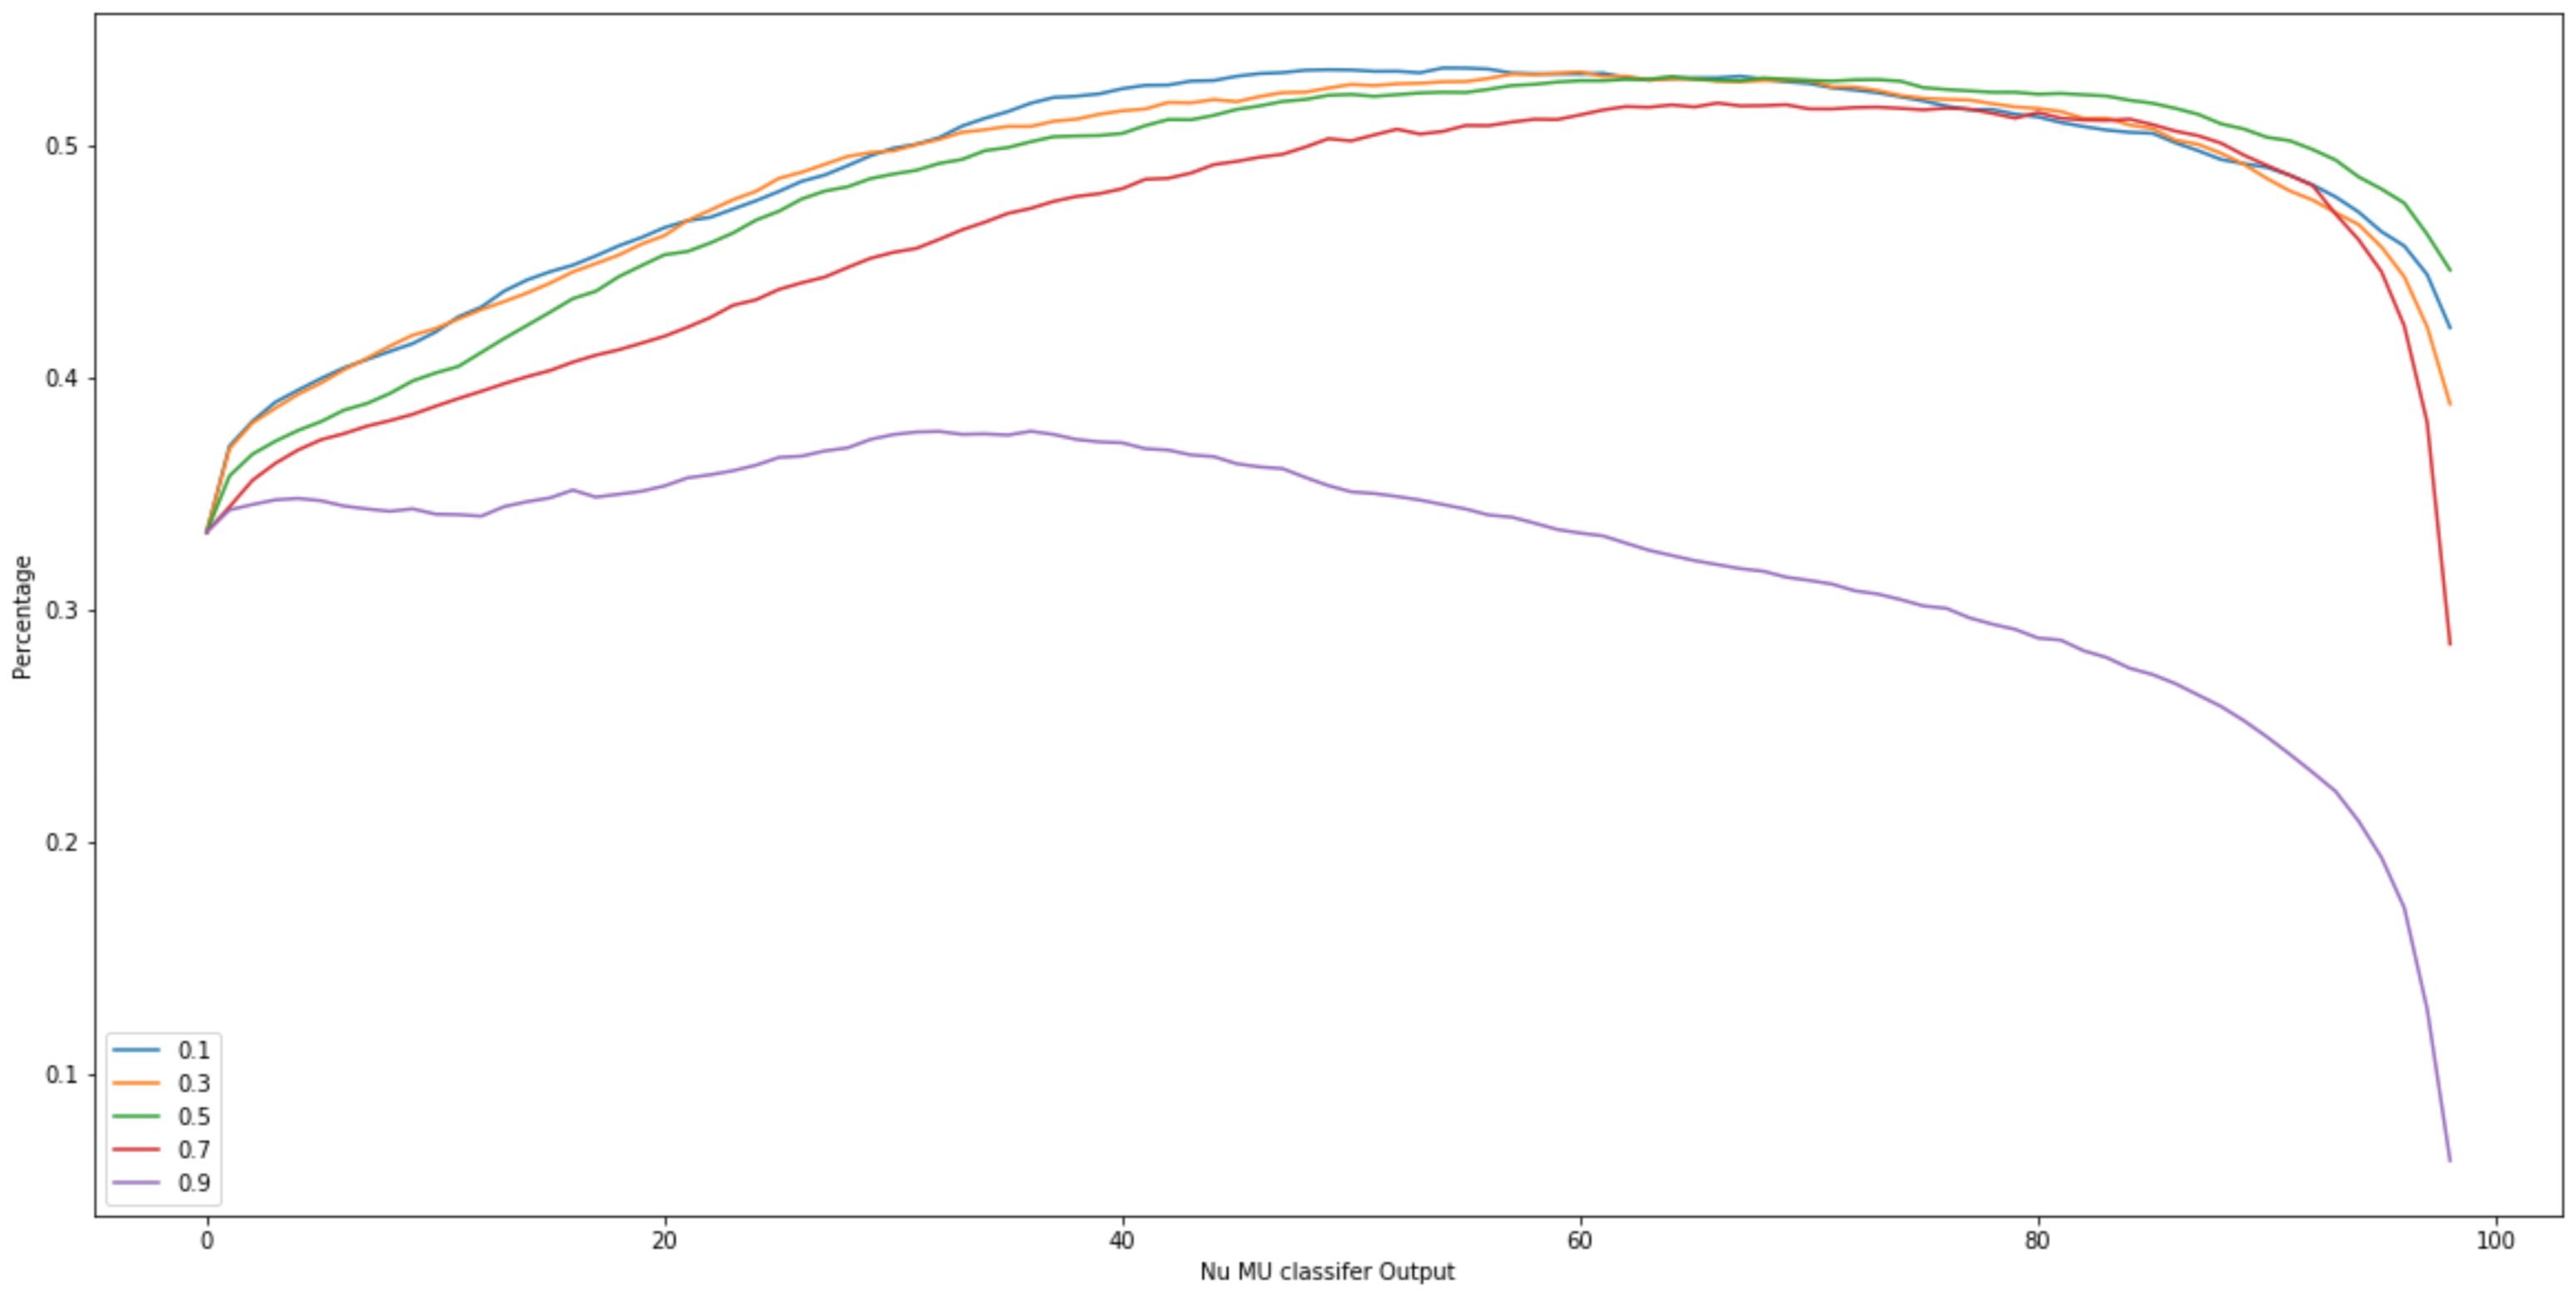
\includegraphics[width=160mm]{dann/dann1.png}
 
 \textbf{Figure 39.} \textit{Purity, efficeny and their product, for DANN $\nu_\mu$ classifier output for DANN gradient reversal scale factors of: 0.1, 0.3, 0.5, 0.7 and 0.9}

 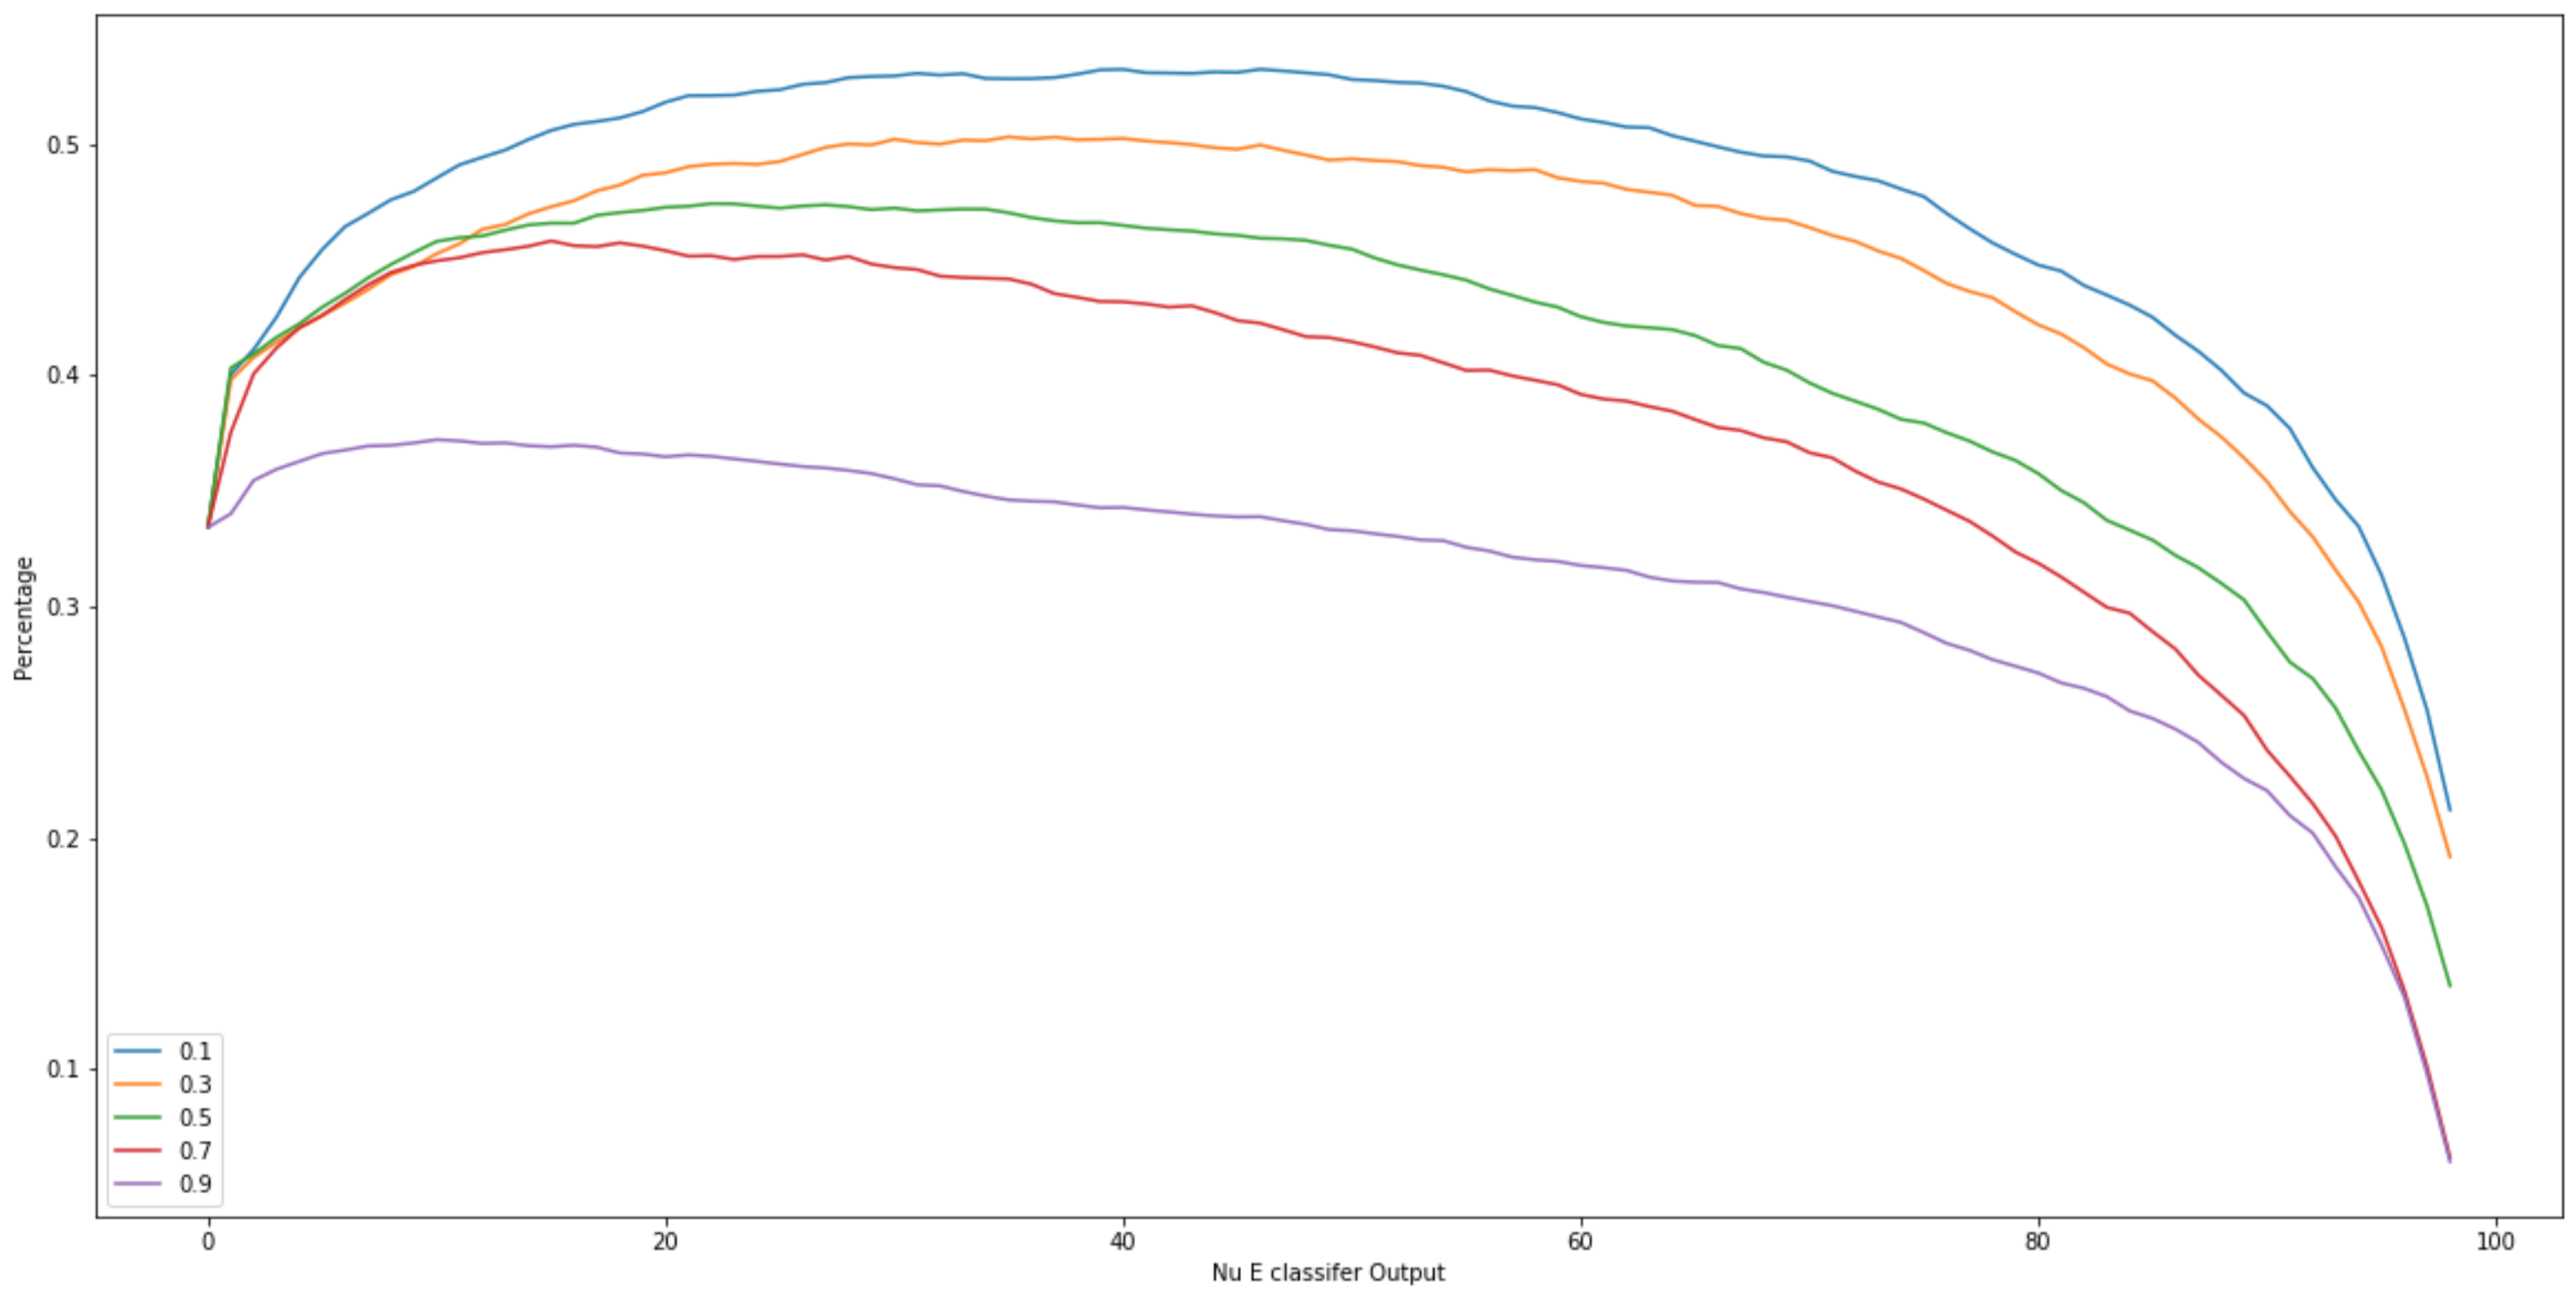
\includegraphics[width=160mm]{dann/dann2.png}
 
 \textbf{Figure 40.} \textit{Purity, efficeny and their product, for DANN $\nu_e$ classifier output for DANN gradient reversal scale factors of: 0.1, 0.3, 0.5, 0.7 and 0.}
\end{figure}

\noindent Scaling factors between 0 and 1, at 0.1, 0.3, 0.5, 0.7 and 0.9, were used in the training process of each model. Again the models were trained, validated and tested on a dataset containing an equal number of each of the three interaction event types, and an equal number of events produced by GiBUU and GENIE. The results of the $\nu_\mu$ classifier are in Figure 39, and show that the performance of the model does reduce as the gradient reversal scaling factor increases. For the smaller values this difference is very small, but as the values increase, the detrimental effect of the gradient reversal has a larger effect on the classification accuracy. This reduction in classification performance can also be seen in the $\nu_e$ classifier in Figure 40. Here the reduction in performance is much larger as the scaling factor increases. \medskip

\noindent This is as expected, in order for the network to become less sensitive to the domain in which the events are being produced, the network is likely to reduce in accuracy as certain events that were easily identified as an interaction type in one of the domains are now being penalised for having such distinctive features. This trade off in classification performance is beneficial however, as the model does not specialise to these distinctive features of the domain, and is better suited to evaluate events from a different domain.\medskip


\noindent In having a more robust model, the difference in classification performance of the model for events from the different domains would tend to zero. This would be as the model performs equally well on events produced by either domain, and thus is invariant to any differences between the two. In Figure 41 a ROC curve is plotted to show the $\nu_\mu$ classification performance for the models of varying gradient scale factors. Different curves were used to plot the performance of events from the two different sources, with solid lines corresponding to GiBUU generated events, and dashed lines for GENIE events, with the colours representing the scale factor used for the training process. While it is very small, it can be seen that the difference in classification performance between the GENIE and GiBUU events does reduce as the scale factor increases. The classification of GENIE events can be seen to increase as the scale factor strength increases, indicating that the model, which previously became overly specialised to GiBUU event features was not less dependent on these which were not found in GENIE events. This does suggest that the $\nu_\mu$ classifier does become more robust as a DANN training process with a larger scale factor takes place- however it is a very small change and would most likely not be considered a negligible improvement when compared to statistical noise. Not all the scale factor training processes were used as the Figure became unreadable, and the scale factor of 0.9 was not used due to it being an exceptionally poor classifier, as seen in Figure 40.\medskip

\begin{figure}[t!]
 \centering
 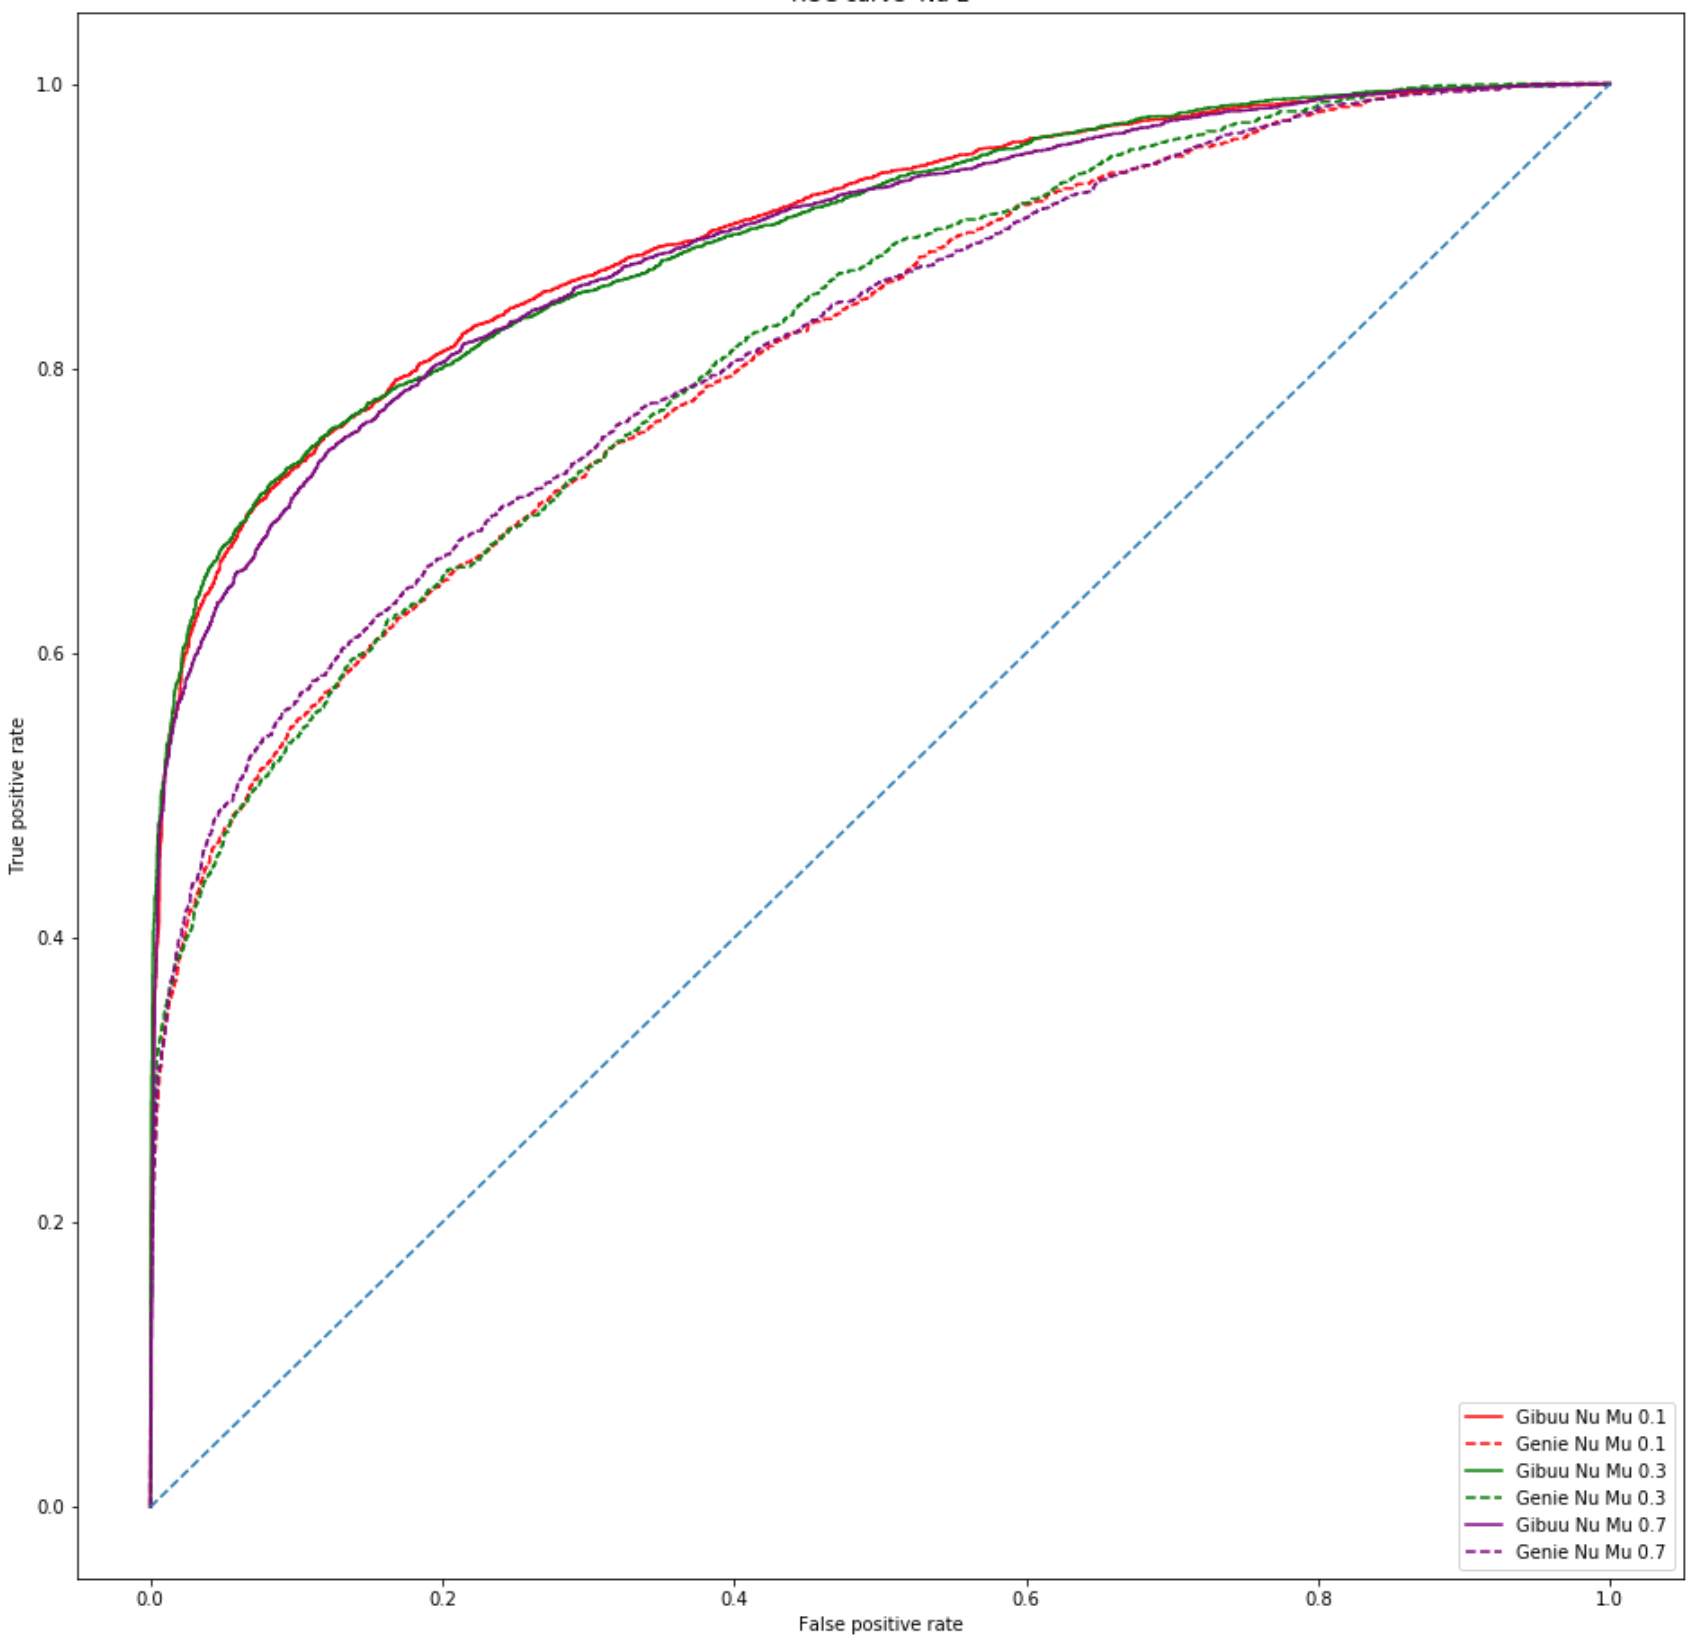
\includegraphics[width=160mm]{dann/dann3.png}
 
 \textbf{Figure 41.} \textit{ROC curve for for DANN $\nu_\mu$ classifier, for DANN gradient reversal scale factors of: 0.1, 0.3, and 0.7, where the GiBUU events are plotted with solid lines and the GENIE curves with dotted lines)}
\end{figure}

\begin{figure}[t!]
 \centering
 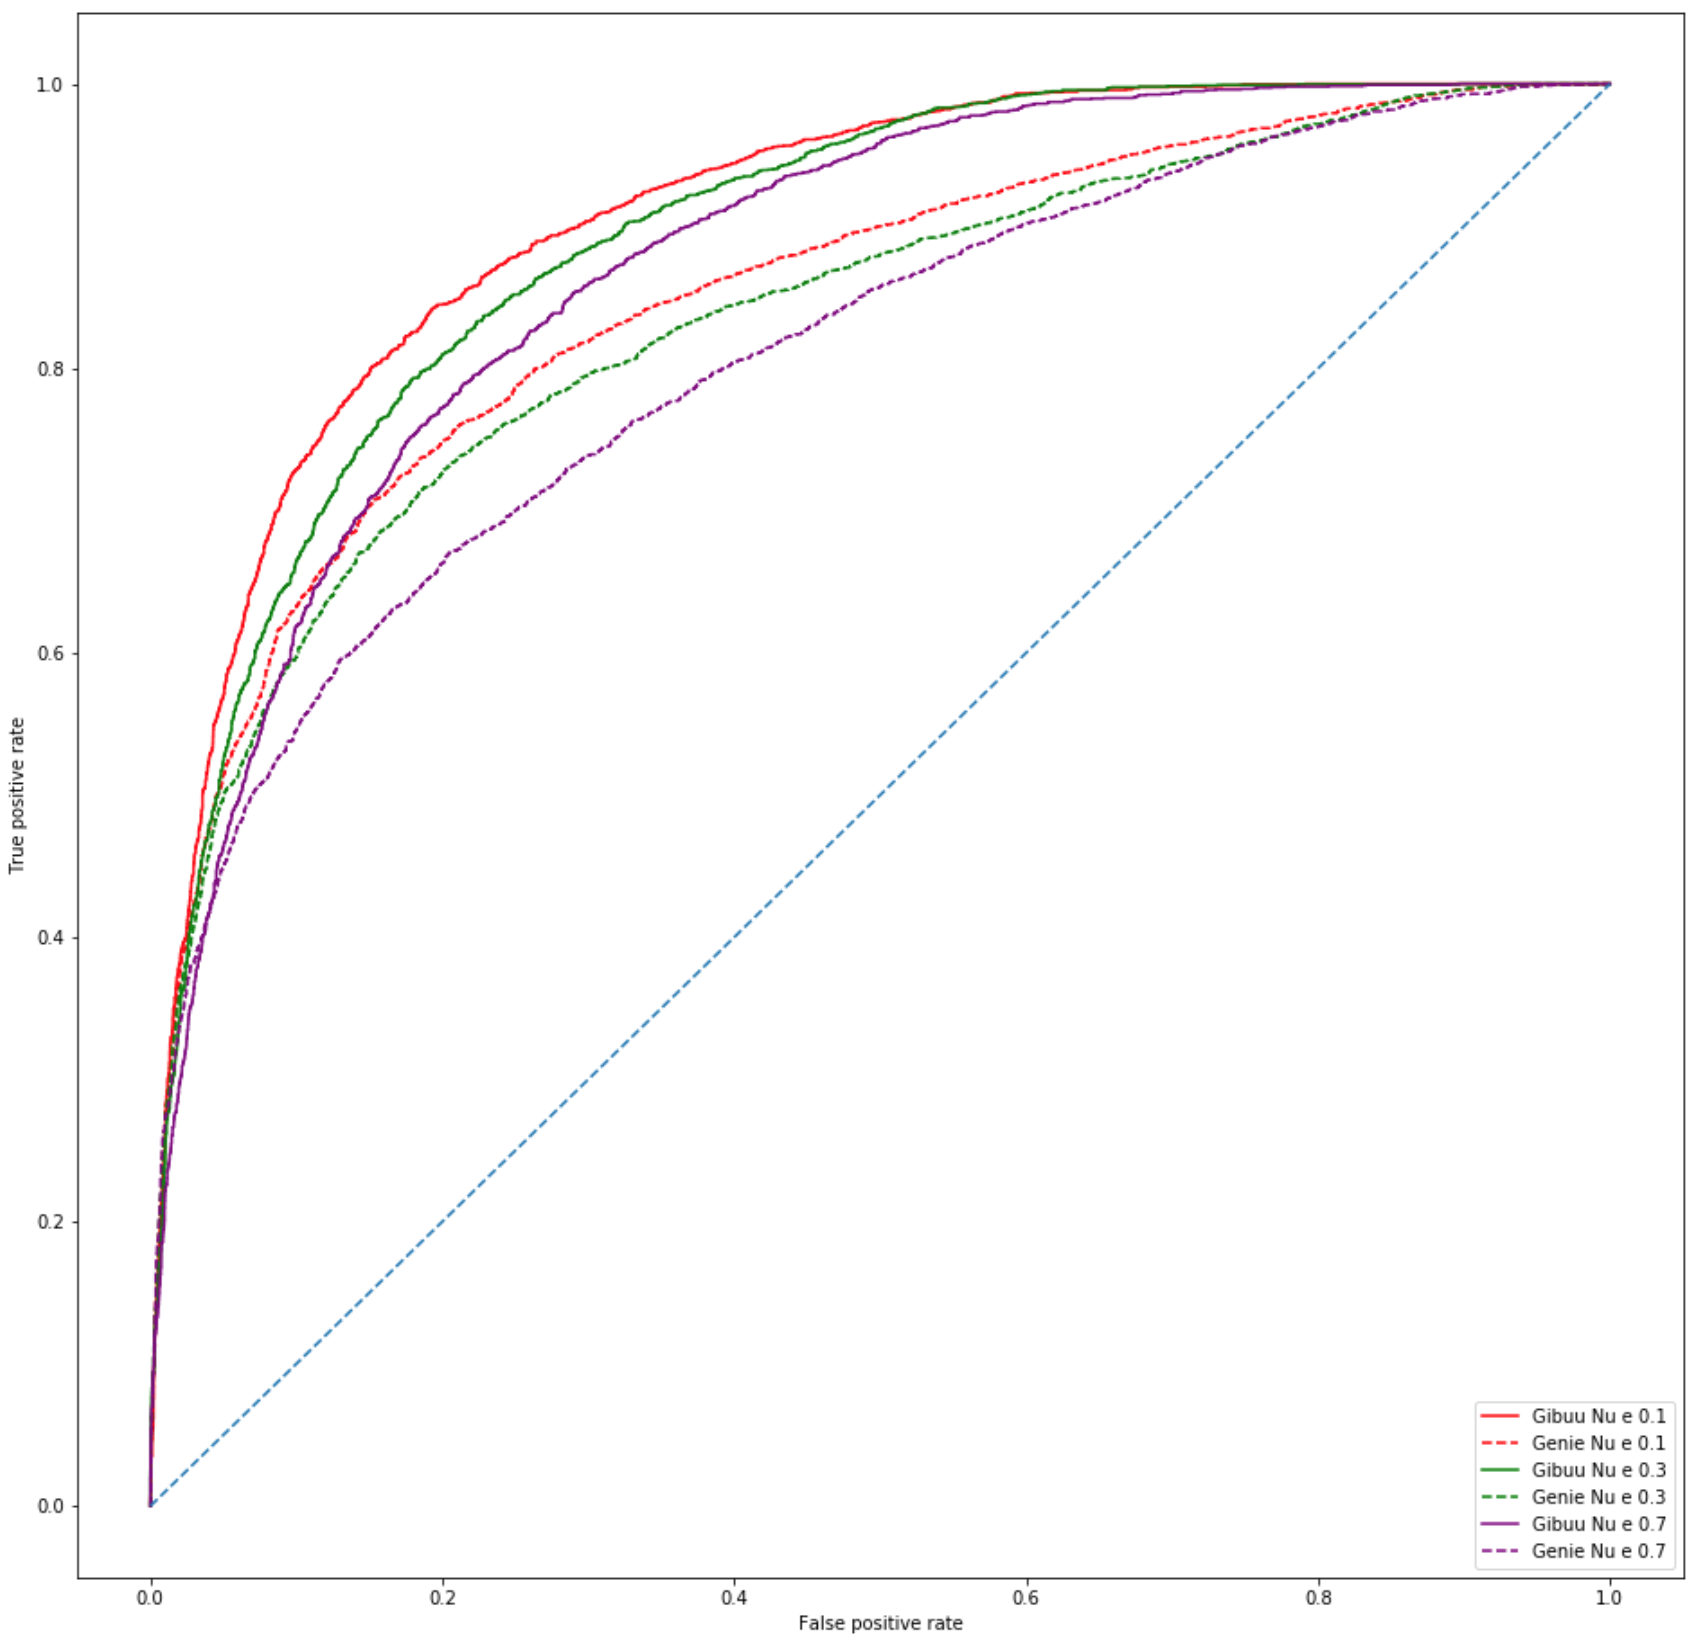
\includegraphics[width=160mm]{dann/dann4.png}
 
 \textbf{Figure 42.} \textit{ROC curve for for DANN $\nu_e$ classifier, for DANN gradient reversal scale factors of: 0.1, 0.3, and 0.7, where the GiBUU events are plotted with solid lines and the GENIE curves with dotted lines}
\end{figure}


\noindent This same increase in robustness cannot be seen by the the $\nu_e$ classifier, Figure 41, where the increase in the strength of the DANN gradient reversal resulted in an overall poorer performance on events produced by both GENIE and GiNUU, with this reduction in performance proportional to the strength of the gradient reversal scale factor. The performance reduces considerably, meaning that the DANN has reduced the network's ability to classify $\nu_e$ events by penalising any ability the network had at discriminating between the two domains. In Figure [], the $\nu_e$ classifier trained on GENIE data performed more poorly when then tested on GiBUU data, indicating that there was a difference the features in the image of a GENIE and GiBUU produced $\nu_e$. The DANN was unable to reduce the difference in classifier performance between events produced from the two domains, suggesting that the $\nu_e$ events now became more difficult to determine now that domain training took place.\medskip


\noindent Figure 36 showed that the nature of the events that were easily identifiable as GiBUU events nearly completely comprised of $NC$ and $\nu_e$ events. The result of successful DANN training would mean that these easily identifiable GiBUU events would result in a negative gradient that backpropagated to make these events less easily identifiable by the network. The proportion of events that were easily identified as being produced by GiBUU that were $\nu_\mu$ events was only 16\%, and thus the DANN process, with regards to these domain identifiable events, was much more limited, which is one reason as to why the DANN process did not reduce the performance of the $\nu_\mu$ classifier. By making the features of these $NC$ and $\nu_e$ events have a reduced impact on the classification process of the network, the network as a result became less successful at identifying these events. \medskip

\noindent This is very straightforward to follow as to how the GiBUU $\nu_e$ performance would have been reduced, but the GENIE performance also fell, leading to a poorer classifier, rather than a more robust one. This may be due to difficulties that are currently the case in classification of GENIE events, such as some $NC$ events looks similar to $\nu_\mu$ events and other similar $\nu_\e$ as displayed in previous sections, but further work would be required to provide insight into this.\medskip



 
\addtocontents{toc}{\vspace{-0.1cm}}
\chapter{Conclusions}
\onehalfspacing

\section{Model Classification}

\noindent This project was able to demonstrate that CNNs are effective tools that can be used to classify neutrino interaction types from image data supplied by MC event simulation generators. Analysis was able to show that there are significant differences in how the two generators GENIE and GiBUU simulate $NC$ and $\nu_e$ events, and these differences impact the classification of events when using a classifier has been trained on one generator and tested on the other/both, or if the classifier is trained on both. \medskip

\noindent While the datasets used in this project were balanced, it is unsure whether applying these models to unbalanced test data provided at the near detector at NO$\va$A would produce results that are not reflective of reality- that over predict the occurrence of $NC$ and $\nu_e$ events due to their much larger prominence in the training data than is the case. Training unbalanced dataset is an ongoing difficulty of machine learning, and one where further research could be applied following on from this project.\medskip

\noindent By analysing the penultimate dense layer activation values when test data was passed through the model, the physical properties of those events that contained domain bias was produced, giving insight into how deep learning classifiers of such events are made less accurate due a domain biases.

\noindent By looking at using the same network architecture to produce a classifier that was able to discern the production source of events, the opportunity for a DANN to reduce this domain bias was displayed. A DANN network was trained using various gradient reversal strength factors and was able to improve the model robustness for $\nu_\mu$ events, but future work may lead to such improvements for $\nu_e$ events. The partial success DANN network stands as a proof of concept that the method can prove effective, and with more work, and more data, a DANN could be a very powerful tool to reduce domain bias in classification models.\medskip

\section{Future Work}

\noindent There are a number of potential avenues for future work following on from this project. One is looking at how penultimate layer analysis can be used to further the field of machine learning explain-ability. Machine learning, and in particular, deep learning algorithms are viewed as black boxes that are given inputs and produce outputs, but methods such as those attempted in this project display that insights into how these algorithms make their decisions can be interpreted.\medskip

\noindent A potential technique to improve the classification accuracy of the model would be one in which chosen penultimate layer nodes were frozen out. This project did not allow the time to explore this, but by writing custom gradient layers, much like the gradient reversal layer implemented in the DANN, to zero back propagation from those selected nodes, but removing the impact of nodes that activated to indicate domain variation, may improve the classification result of the network if the classification features were the only ones that were used within the network.\medskip

\noindent As with all supervised machine learning algorithms, improvements are made when more data is provided to the network in the training process. Further work would be to train classifiers, domain classifiers and DANN models with larger amounts of input data, and potentially better hard were to accelerate this process to reduce the problem of overfitting due to small amounts of data, leading the networks to pick up on statistical noise. An alternative to this, to reduce the ill-posed nature of the problem would be to attempt to use a network architecture with a smaller number of trainable parameters. This network may be less powerful than the MobileNet architecture base used in this project, however it would be far less susceptible to overfitting.\medskip

\noindent Using a DANN to train inputs of both simulated data and detector data would be the next step to have a major impact at NO$\nu$A and improve the computer vision classifier already being used there to improve the accuracy of the data being used in neutrino oscillation calculations. \medskip

\noindent Further work could be carried out into understanding the results of the DANN network, and how one may be able to improve the accuracy of the network. An alternate ADDA method has been produced by \cite{Tzeng}, that encodes the labels in the source domain and a separate encoding that maps target labels to the same space using a mapping learned though a domain-adversarial loss. This could be another avenue of research for the problem of domain bias reduction.\medskip

\noindent In order to produce more training data there is the potential for a form of data augmentation, where small changes- an example would be a Gaussian blur, are applied to the training data to produce new training data from the original training set. This would be especially useful for $\nu_e$ events, where the proportion of data simulated at the near detector is much smaller than that of $\nu_\mu$ events.\medskip



\addtocontents{toc}{\vspace{0.3cm}}

\addtocontents{toc}{\textbf{5 \enspace Bibliography \enspace  \enspace \enspace  \enspace  \enspace  \enspace  \enspace
\enspace \enspace  \enspace  \enspace  \enspace  \enspace  \enspace  \enspace \enspace  \enspace  \enspace  \enspace
\enspace \enspace  \enspace  \enspace  \enspace  \enspace   \enspace \enspace  \enspace  \enspace  \enspace  \enspace
\enspace \enspace  \enspace  \enspace  \enspace  \enspace 
\enspace \enspace  \enspace  \enspace  \enspace  \enspace 
\enspace \enspace  \enspace  \enspace  \enspace  \enspace  \enspace  \enspace \enspace  \enspace  \enspace  \enspace
\enspace \enspace  \enspace  \enspace    50}}

\begin{thebibliography}{}

\bibitem{Vitagliano} 
E. Vitagliano, J. Redondo, G. Raffelta et al.
\textit{Solar neutrino flux at keV energies}. 
2017.

\bibitem{Maki} 
Z. Maki, M. Nakagawa, S. Sakata et al.
\textit{Remarks on the Unified Model of Elementary Particles}. 
1962.

\bibitem{Szadowski} 
Z. Szadowski, D. Glas, K. Pytel et al.
\textit{Artificial Neural Networks as a FPGA Trigger for a Detection of Neutrino-Induced Air Showers}. 
2016.

\bibitem{Perdue} 
G.N Perdue, A. Ghosh, M. Wospakrik et al.
\textit{Reducing model bias in a deep learning classifier using domain adversarial neural networks in MINER$\nu$A experiment}. 
2018.

\bibitem{Brenzke} 
M. Brenzke
\textit{Development and Optimization of Deep Neural Networks for Energy Reconstruction of Muon Events in IceCube}. 
2017.

\bibitem{Fukuda_1} 
 Y. Fukud, T. Hayakawa, E. Ich. et al.
\textit{The Super-Kamiokande detector}.
2002.



\bibitem{Acciarri_1} 
R. Acciarri, M. A. Acero, M. Adamowski et al.
\textit{Long-Baseline Neutrino Facility (LBNF) and Deep Underground Neutrino Experiment (DUNE) Conceptual Design Report Volume 1: The LBNF and DUNE Projects}. 
2016.

\bibitem{Aurisano} 
A. Aurisano, A. Radovic, D. Rocco et al.
\textit{A Convolutional Neural Network Neutrino Event Classifier}. 
2016.

\bibitem{Fukuda_2} 
Y. Fukuda , T.Hayakawa , E.Ichihara et al.
\textit{Evidence for oscillation of atmospheric neutrinos}. 
1998.

\bibitem{Capozzi} 
F. Capozzi, E. Lisi and A. Marrone et al.
\textit{Neutrino masses and mixings: Status of known and unknown 3$\nu$ parameters}. 
2016.
\bibitem{Giganti} 
C. Giganti, S. Lavignac, M. Zito et al.
\textit{Neutrino oscillations: the rise of the PMNS paradigm}. 017

\bibitem{Sonneveld} 
J. Sonneveld
\textit{Searches for physics beyond the standard model at the LHC}. 
2018.

\bibitem{Ishitsuka} 
M. Ishitsuka et al.
\textit{NOvA Near Detector}.

\bibitem{Singh} 
P. Singh
\textit{Extracting neutrino oscillation parameters using a simultaneous fit of the $\nu_e$ appearance and $\nu_\mu$ disappearance data in the NOvA experiment}.
2017.

\bibitem{Szegedy} 
C. Szegedy, C. Hill  and Y. Jia et al.
\textit{Going deeper with convolutions}. 
2014.

\bibitem{Adamson_1} 
P. Adamson, C. Ader and M. Andrews et al.
\textit{First measurement of muon-neutrino disappearance in NOvA}. 
2016.

\bibitem{Adamson_2} 
P. Adamson, C. Ader and M. Andrews et al.
\textit{First measurement of muon-neutrino appearance in NOvA}. 
2016.

\bibitem{McCulloch} 
W. McCulloch and W. Pitts. 
\textit{A Logical Calculus of Ideas Immanent in Nervous Activity}. 
1943.

\bibitem{Andreopoulos_1} 
C. Andreopoulos , C. Barry , S. Dytman et al.
\textit{The GENIE Neutrino Monte Carlo Generator PHYSICS \& USER MANUAL}. 
2015.

\bibitem{Andreopoulos_2} 
C.Andreopoulos , A.Bellb, D.Bhattacharyab et al.
\textit{The GENIE Neutrino Monte Carlo Generator}. 
2009.

\bibitem{Lalakulich} 
O. Lalakulich, K. Gallmeister, U. Mosel et al.
\textit{Neutrino nucleus reactions within the GiBUU model}. 
2011.

\bibitem{Acciarri_2} 
R. Acciarri, C. Adams, R. An et al.
\textit{Convolutional neural networks applied to neutrino events in a liquid argon time projection chamber}. 
2017.

\bibitem{Sandler} 
M. Sandler, A. Howard, M. Zhu et al.
\textit{MobileNetV2: Inverted Residuals and Linear Bottlenecks}.2018

\bibitem{Ganin} 
Y. Ganin, E. Ustinova, H. Ajakan et al.
\textit{Domain-Adversarial Training of Neural Networks}.
2016. 

\bibitem{Kingma} 
D. Kingma, J. Ba.
\textit{Adam: A Method for Stochastic Optimization}.
2014. 

\bibitem{Zhang} 
Q. Zhang, Y. Nian Wu,  S. Zhu et all
\textit{Interpretable Convolutional Neural Networks}.
2018. 

\bibitem{Bousmalis} 
Z. Bousmalis, G. Trigeorgis, N. Silberman et al.
\textit{Domain Separation Networks}.
2016.

\bibitem{Louppe} 
G. Louppe, M. Kegan K. Crammer et al.
\textit{Learning to Pivot with Adversarial Neural Networks}.
2017.

\bibitem{Brun} 
R. Brun, F. Rademakers et al.
\textit{ROOT - An object oriented data analysis framework}.
1997.

\bibitem{Tzeng}
E. Tzeng, J. Hoffman, K. Saenko et al.
\textit{Adversarial Discriminative Domain Adaptation}
2017

\bibitem{Guo}
H. Guo and S. B. Gelfand,
\textit{Analysis of gradient descent learning algorithms for multilayer feedforward neural networks}.
1990.
\end{thebibliography}

\addtocontents{toc}{\newline}
\addtocontents{toc}{\largeskip}
\addtocontents{toc}{\vspace{-0.2cm}}

\addtocontents{toc}{\textbf{6 \enspace Appendices - Source Code  \enspace \enspace  \enspace  \enspace  \enspace  
\enspace \enspace  \enspace  \enspace  \enspace  \enspace  \enspace  \enspace \enspace  \enspace  \enspace  \enspace
\enspace \enspace  \enspace  \enspace  \enspace  \enspace   \enspace \enspace  \enspace  \enspace  \enspace  \enspace
\enspace \enspace  \enspace  \enspace  \enspace  \enspace 
\enspace \enspace  \enspace  \enspace  \enspace  \enspace 
\enspace \enspace  \enspace  \enspace  \enspace  \enspace  \enspace  52}}


\onehalfspacing
\newpage
\chapter*{Appendices - Source Code}

\section*{functions.py}

\begin{lstlisting}[language=Python]
import h5py
import numpy as np
import copy
import pandas as pd
import random
import pickle as pkl
import mobilenetv2
import tensorflow as tf
import keras
from keras.optimizers import SGD, Adam
from keras.callbacks import EarlyStopping, ModelCheckpoint

def encode_event(array, i):
    """encode_event
    Function that takes in an hdf5 array and an index gives the run, subrun, evt, subevt, cycle of an event
    and returnsthem as a string for quick lookups
    # Arguments
        array: branch from the hdf5 files
        i: index within the array
    # Returns
	string containing run, subrun, evt, subevt, cycle
    """
    run = array['run'][i]
    subrun = array['subrun'][i]
    evt = array['evt'][i]
    subevt = array['subevt'][i]
    cycle = array['cycle'][i]
    try:
        genweight = array['genweight'][i]
        arr_str = ('{},{},{},{},{},{}'.format(run, subrun, evt, subevt, cycle, genweight))
    except KeyError:
        arr_str = ('{},{},{},{},{}'.format(run, subrun, evt, subevt, cycle))
    return arr_str



def get_files(path):
    """get_files
    Function creates a list of all the hdf5 files in a directorty
    # Arguments
        path: the path to the direectory
    # Returns
	filenames: list of filenames"""
    folder = os.listdir(os.fsencode(path))
    filenames = [os.fsdecode(file) for file in folder if os.fsdecode(file).endswith(('.h5'))]

    return filenames



def data(file):
    """data
    Function that extracts the data from the hdf5 file and returns the relevant data
    # Arguments
        file: hdf5 file name
    # Returns
	f - the hfd5 file
        file - hfd5 file name
        Train_Params - a dictionary with keys = [run, subrun, evt, subevt, cycle] and
        values = [train array index, iscc value, pdg value]
        maps - the arrays containing the image data
        cvnmaps - the branch of the hdf5 file that contains the maps
    """
    #import file
    f = h5py.File(file, 'r')

    # cvn training data branch and truth branch keys
    cvnmaps = f['rec.training.cvnmaps']
    mc = f['rec.mc.nu']
    train_event = [encode_event(cvnmaps, i) for i in range(len(cvnmaps['evt']))]
    mc_event = [encode_event(mc, i) for i in range(len(mc['evt']))]

    #mapping
    Train_Params = {}
    for i in range(len(mc_event)):
        for j in range(len(train_event)):
            #only including the run, subrun, evt, subevt, cycle data from the mc branch in the matching
            mc_data  = ','.join(mc_event[i].split(',')[:-1])
            train = train_event[j]
            if mc_data == train:
                Train_Params[mc_event[i]] = j, mc['iscc'][i][0], mc['pdg'][i][0]

    return f, file, Train_Params



def mu_cuts(f, file):
    """
    Function that takes in an hdf5 file and creates a list of events that do not pass the nu mu cuts:
    nu mu cuts defined - "CAFAna/Cuts/NumuCuts2018.h"
        cuts used - kNumuQuality && kNumuContainFD2017
    """
    files_list = [os.fsdecode(file) for file in folder if os.fsdecode(file).endswith(('.h5'))]
    cut_arr_mu = []

    ### kNumuQuality cut ###
    en_numu = f['rec.energy.numu']
    for i in range(len(en_numu['trkccE'])):
        if en_numu['trkccE'][i]<=0:
            s = encode_event(en_numu, i)
            if s not in cut_arr_mu:
                cut_arr_mu.append(s)

    cut = [encode_event(sel_remid, i) for i in len(en_numu['trkccE']) if en_numu['trkccE'][i]<=0]
    s = encode_event(cut, i)
    if s not in cut_arr_mu:
        cut_arr_mu.append(s)

    sel_remid = f['rec.sel.remid']
    for i in range(len(sel_remid['pid'])):
        if sel_remid['pid'][i]<=0:
            s = encode_event(sel_remid, i)
            if s not in cut_arr_mu:
                cut_arr_mu.append(s)

    slc = f['rec.slc']
    for i in range(len(slc['nhit'])):
        if slc['nhit'][i]<=20 or slc['ncontplanes'][i]<=4:
            s = encode_event(slc, i)
            if s not in cut_arr_mu:
                cut_arr_mu.append(s)

    cosmic = f['rec.trk.cosmic']
    for i in range(len(cosmic['ntracks'])):
        if cosmic['ntracks'][i]<=0 :
            s = encode_event(cosmic, i)
            if s not in cut_arr_mu:
                cut_arr_mu.append(s)

    ### kNumuContainFD2017 cut ###
    shwlid = f['rec.vtx.elastic.fuzzyk.png.shwlid']
    for i in range(f['rec.vtx.elastic.fuzzyk.png.shwlid']['start.x'].shape[1]):
        a = min(shwlid['start.x'][i],shwlid['stop.x'][i])
        b = max(shwlid['start.x'][i],shwlid['stop.x'][i])
        c = min(shwlid['start.y'][i], shwlid['stop.y'][i])
        d = max(shwlid['start.y'][i], shwlid['stop.y'][i])
        e = min(shwlid['start.z'][i], shwlid['stop.z'][i])
        f = max(shwlid['start.z'][i], shwlid['stop.z'][i])
        if a <=-180 or b >=180 or c <=-180 or d >=180 or e <=20 or f >=1525:
            s = encode_event(shwlid, i)
            if s not in cut_arr_mu:
                cut_arr_mu.append(s)

    f = h5py.File(file, 'r')
    kal_track = f['rec.trk.kalman.tracks']
    for i in range(len(kal_track['start.z'])):
        if kal_track['start.z'][i]>1275 or kal_track['stop.z'][i]>1275:
            s = encode_event(kal_track, i)
            if s not in cut_arr_mu:
                cut_arr_mu.append(s)

    slc = f['rec.slc']
    for i in range(len(slc['firstplane'])):
        if slc['firstplane'][i]<=1 or slc['lastplane'][i]==212 or slc['lastplane'][i]==213:
            s = encode_event(slc, i)
            if s not in cut_arr_mu:
                cut_arr_mu.append(s)

    sel = f['rec.sel.contain']
    for i in range(len(sel['kalfwdcellnd'])):
        if sel['kalyposattrans'][i]>=55 or sel['kalbakcellnd'][i]<10 or sel['kalfwdcellnd'][i]<5:
            s = encode_event(sel, i)
            if s not in cut_arr_mu:
                cut_arr_mu.append(s)

    return cut_arr_mu



def apply_cuts(Train_Params, cut_arr, file):
    """apply_cuts
    Function that the list of cut events and removes them from the mctruth events dictionary
    # Arguments
        Train_Params: the dictionary of events containing iscc and pdg data
        cut_arr: the list of events that did not pass the cuts
    # Returns
	Train_Params_Cut: the new dictionary of events
        events: the training data branch array index values of the events that passed the cut
        train: 2-dimential array, iscc, pdg
        train_val: 1-dimential array, iscc
    """
    Train_Params_Cut= copy.deepcopy(Train_Params)
    for i in cut_arr:
        if i in Train_Params_Cut.keys():
            del Train_Params_Cut[i]

    dataframes = []
    for key in Train_Params_Cut.keys():
        iscc = Train_Params_Cut[key][1]
        pdg = Train_Params_Cut[key][2]
        if iscc == 0:
            interaction = 1
        elif iscc == 1 and pdg*pdg ==144:
            interaction = 2
        elif iscc == 1 and pdg*pdg ==196:
            interaction = 3

        key_split = key.split(',')
        run = key_split[0][1:-1]
        subrun = key_split[1][1:-1]
        evt = key_split[2][1:-1]
        subevt = key_split[3][1:-1]
        cycle = key_split[4][1:-1]
        weight = key_split[5][1:-1]

        dataframes.append(pd.DataFrame({'run' : run,
                                        'subrun' : subrun,
                                        'evt' : evt,
                                        'subevt' : subevt,
                                        'cycle' : cycle,
                                        'weight': weight,
                                        'train_index' :  Train_Params_Cut[key][0],
                                        'label' : interaction,
                                        'file' : [file]
                                       }))

    df = pd.concat(dataframes)

    return df



def e_cuts(f, file):
    """e_cuts
    Function that takes in an hdf5 file and creates a list of events that do not pass the nu e cuts:
    nu mu cuts defined - "CAFAna/Cuts/NueCuts2017.h"
        cuts used - kNue2017NDFiducial && kNue2017NDContain && kNue2017NDFrontPlanes
    """
    ## Nu E Preselection Cuts  #
    cut_arr_e = []

    f = h5py.File(file, 'r')
    # kNue2017NDFiducial
    vtx_el = f[ 'rec.vtx.elastic']
    for i in range(len(vtx_el['vtx.x'])):
        a= vtx_el['vtx.x'][i]
        b= vtx_el['vtx.y'][i]
        c= vtx_el['vtx.z'][i]
        if a<=-100 or a>=160 or b<=-160 or b>=100 or c<=150 or c>=900:
            s = encode_event(vtx_el, i)
            if s not in cut_arr_e:
                cut_arr_e.append(s)

    # kNue2017NDContain
    shwlid = f['rec.vtx.elastic.fuzzyk.png.shwlid']
    for i in range(len(f['rec.vtx.elastic.fuzzyk.png.shwlid']['start.x'])):
        a = min(shwlid['start.x'][i],shwlid['stop.x'][i])
        b= max(shwlid['start.x'][i],shwlid['stop.x'][i])
        c= min(shwlid['start.y'][i], shwlid['stop.y'][i])
        d= max(shwlid['start.y'][i], shwlid['stop.y'][i])
        e = min(shwlid['start.z'][i], shwlid['stop.z'][i])
        f= max(shwlid['start.z'][i], shwlid['stop.z'][i])
        if a <=-170 or b >=170 or c <=-170 or d >=170 or e <=100 or f >=1225:
            s = encode_event(shwlid, i)
            if s not in cut_arr_e:
                cut_arr_e.append(s)
        pass

    # kNue2017NDFrontPlanes
    f = h5py.File(file, 'r')
    sel = f['rec.sel.contain']
    for i in range(len(sel['nplanestofront'])):
        if sel['nplanestofront'][i]<=6:
            s = encode_event(sel, i)
            if s not in cut_arr_e:
                cut_arr_e.append(s)

    return cut_arr_e



def maps(file):
    """maps Function that returns event maps from the hdf5 file
    # Arguments, file: hdf5 file name
    # Returns, maps - the arrays containing the image data
    """
    #import file
    f = h5py.File(file, 'r')

    # cvn training data branch
    cvnmaps = f['rec.training.cvnmaps']
    maps = cvnmaps['cvnmap']

    return maps



def image(maps):
    """image
    Function that the array containing the images and formats them correctly
    # Arguments
        maps: the array containing the images
    # Returns
	image_dataset: nested array containing two images for each event for the z-y and z-x planes
    """
    image_dataset = np.zeros(shape=(2,80,100))
    image_dataset[0,:,:] = np.rot90(np.asarray(maps[:8000]).reshape(100,80))
    image_dataset[1,:,:] = np.rot90(np.asarray(maps[8000:]).reshape(100,80))

    return image_dataset



def event(data, label):
    """event
    Function that takes in an array of event images and displays them
    # Arguments
        data: image array
        i: index within the array
    # Returns
	plot of image along with associated data
    """
    #first view z-x plane
    raw_im_1_cc = data[0,:,:]
    #second view z-y plane
    raw_im_2_cc = data[1,:,:]

    fig, (ax1, ax2) = plt.subplots(2, 1, figsize=(9, 9))

    #axis lables
    ax1.imshow(raw_im_1_cc, aspect='auto')
    ax1.set_xlabel('z (units)')
    ax1.set_ylabel('x (units)')
    ax2.imshow(raw_im_2_cc, aspect='auto')
    ax2.set_xlabel('z (units)')
    ax2.set_ylabel('y (units)')
    fig.suptitle(label)



def open_df(path, num):
    """open_df
    Function that takes in a folder path and a number and unpickles the assosiated dataframe
    # Arguments
        path: path to the folder containing pickled dataframes
        num: dataframe number, e.g. df_1.pkl
    # Returns
	the dataframe containing the associated data
    """
    with open(path+ 'df_{}.pkl'.format(num),'rb') as file:
        df = pkl.load(file)
    return df



def open_df_gibuu(path, num):
    """open_df_gibuu
    Function that takes in a folder path and a number and unpickles the assosiated dataframe
    # Arguments
        path: path to the folder containing pickled dataframes
        num: dataframe number, e.g. df_gibuu_1.pkl
    # Returns
	the dataframe containing the associated data
    """
    with open(path+ 'df_gibuu_{}.pkl'.format(num), 'rb') as file:
        try:
            df = pkl.load(file)
            return df
        #some gibuu file dataframes were not correctly saved, leading to Unpickling Errors
        except pkl.UnpicklingError:
            print('Unpickling Error with gibuu df file {}'.format(num))
            pass


def generator(batch_size, steps_per_epoch, dataset, model = 'default'):
    """generator
    Generator function that yeilds a tensor contraining image data and the associated lables to be called by the keras 
    in training of the model
    # Arguments
        batch_size: path to the folder containing pickled dataframes
        steps_per_epoch: dataframe number, e.g. df_gibuu_1.pkl
        dataset: 
        model: 
    # Returns
	batch_images:
	batch_labels:
	batch_events: 
    """
    batch_images = np.zeros((batch_size, 2, 80, 100))
    batch_labels = np.zeros((batch_size, 3))
    batch_events = np.zeros((batch_size, 2))

    while True:
        dataset = dataset.sample(frac=1).reset_index(drop=True)

        for index in range(len(dataset['file'])):
            row = dataset.loc[index]

            images = image(maps(row['file'])[row['train_index']])
            images = (images - np.min(images))/ (np.max(images) - np.min(images))
            images.astype(float)

            if abs(row['label']- 1) <=10**(-5):
                labels = [1, 0, 0]
            elif abs(row['label']- 2) <=10**(-5):
                labels = [0, 1, 0]
            elif abs(row['label']- 3) <=10**(-5):
                labels = [0, 0, 1]

            if '_genie_' in str(row['file']):
                events = [1, 0]
            elif 'gibuu' in str(row['file']):
                events = [0, 1]

            batch_images[index%batch_size] = images
            batch_labels[index%batch_size] = labels
            batch_events[index%batch_size] = events

            if index%batch_size==0 and index!=0:
                if model== 'default':
                    yield batch_images, batch_labels
                elif model== 'descr':
                    yield batch_images, batch_events
                elif model== 'dann':
                    yield batch_images, [batch_labels, batch_events]
          



def test_generator(batch_size, steps_per_epoch, dataset, data='both', model_type = 'default'):

    for index in range(len(dataset['file'])):
        row = dataset.loc[index]
        weight = float(row['weight'])
        file = str(row['file'])
    
        rand = 0
        rand2, rand3 = 1, 1

        if (weight<= rand and 'gibuu' in file) or \
            (rand2 <= 0.98 and abs(float(dataset.loc[index]['label'])-3)<=10**(-5)) or \
            (rand3 <= 0.82 and abs(float(dataset.loc[index]['label'])-1)<=10**(-5)):
            pass
        
        else:
            images = image(maps(row['file'])[row['train_index']])
            images = (images - np.min(images))/ (np.max(images) - np.min(images))

            if '_genie_' in file:
                 mc = [1, 0]
            elif 'gibuu' in file:
                 mc = [0, 1]

            if abs(row['label']- 1) <=10**(-5):
                label = [1, 0, 0]
            elif abs(row['label']- 2) <=10**(-5):
                label = [0, 1, 0]
            elif abs(row['label']- 3) <=10**(-5):
                label = [0, 0, 1]

            yield images, row

			

def index_finder(probabilities, df_row):
	
    genie_index_below = []
    genie_index_above = []
    gibuu_index_below = []
    gibuu_index_above = []
	
    for i , prob in enumerate(probabilities):
        genie = prob[0][0]
	gibuu = prob[0][1]
        if gibuu<0.2:
            gibuu_index_below.append(i)
	elif gibuu>0.4 and gibuu<0.7:
	    gibuu_index_above.append(i)
	if genie<0.2:
            genie_index_below.append(i)
	elif genie>0.4 and gibuu<0.7:
	    genie_index_above.append(i)
		
    df_genie_below = pd.DataFrame(columns = df_row.columns)
    df_genie_above = pd.DataFrame(columns = df_row.columns)
    df_gibuu_below = pd.DataFrame(columns = df_row.columns) 
    df_gibuu_above = pd.DataFrame(columns = df_row.columns)
	
    for i, j in enumerate(genie_index_below):
        df_genie_below.loc[i] = df_row.loc[j]
	df_genie_below['type'] = ['genie below']*len(df_genie_below)
	
    for i, j in enumerate(genie_index_above):
        df_genie_above.loc[i] = df_row.loc[j]
	df_genie_above['type'] = ['genie above']*len(df_genie_above)
	
    for i, j in enumerate(gibuu_index_below):
        df_gibuu_below.loc[i] = df_row.loc[j]
	df_gibuu_below['type'] = ['gibuu below']*len(df_gibuu_below)
	
    for i, j in enumerate(gibuu_index_above):
        df_gibuu_above.loc[i] = df_row.loc[j]
	df_gibuu_above['type'] = ['gibuu above']*len(df_gibuu_above)
	
    frames = [df_genie_below, df_genie_above, df_gibuu_below, df_gibuu_above]
    df = pd.concat(frames)
    df.index = range(len(df['file']))
	
    for index, evt in enumerate(df['evt']):
        file = df['file'][index]
        f = h5py.File(file ,'r')
        mc = f['rec.mc.nu']
        columns = [str(i) for i in mc.keys()]
        df_out = pd.DataFrame(columns = columns)

        for count, val in enumerate(mc['evt']):
            if int(val) == int(evt):
                if int(mc['subevt'][count]) ==  int(df['subevt'][index]):
                    mc_index = count
                    break
            elif int(val)>=int(evt)+1:
                break
        row = [mc[str(i)][mc_index][0] for i in mc.keys()]
        df_out.loc[index] = row

    return df_out

\end{lstlisting}

\section*{methods.py}

\begin{lstlisting}[language=Python]
from functions import *
from mobilenetv2 import *
from keras.models import Model
from itertools import islice


def cuts(path):
    """cuts
    Function that takes in an hdf5 file and applied multiple functions to :
    nu mu cuts defined - "CAFAna/Cuts/NueCuts2017.h"
        cuts used - kNue2017NDFiducial && kNue2017NDContain && kNue2017NDFrontPlanes
    """
    #import files
    file_dir = get_files(path)

    #split input files into batches of 50 files

    batches = [file_dir[i:i+100] for i in range(0, len(file_dir), 100)]
    batch_no = 0

    #for set of 50 files
    for i in batches:
        batch_no+=1

        dataframes = []

        #for file in batch
        for j in i:

            try :
                hdf, file, Train_Params = data(path + '/' + j)

                ######### Cuts #############################################################

                cut_arr_mu = mu_cuts(hdf, file)
                dataframes.append( apply_cuts(Train_Params, cut_arr_mu, file) )

                cut_arr_e = e_cuts(hdf, file)
                dataframes.append( apply_cuts(Train_Params, cut_arr_e, file))

            except OSError:
                pass

        #### Save files #########################################################################

        out_path = '/home/ishokar/dataframes/'

        df = pd.concat(dataframes)
        df.index = range(len(df['file']))

        with open(out_path + '/df_{}.pkl'.format(batch_no),'wb') as f1:
            pkl.dump(df, f1)







def train(train_type = 'default',
          epochs= 200,
          batch_size = 32,
          dataset_percent = 0.8,
          call_back_patience = 10,
          learning_rate = 0.001,
          DANN_strength = 0.1, 
          model_optimiser='SGD',
          out_file_name = '32_SGD'):

    """train_mobnetmodelv2
    Function that compiles and trains the mobilenet network
    # Arguments/Hyperparamaters
        epochs: number of epochs,
        batch_size : batch size,
        learning_rate : learning rate,
        call_back_patience : number of epochs patience before stopping training if no improvement takes place,
        save_best : saves weights of the best model based on validation loss
    # Returns
	mobnetmodel: trained model
        history : training statistics
    """
    path = '/home/ishokar/dataframes/'
    df_train = open_df(path, 'train_equal')
    df_train.index = range(len(df_train['file']))
    steps_per_epoch = round(len(df_train['file'])/(batch_size)*dataset_percent)
    
    df_val = open_df(path, 'val_equal')
    df_val.index = range(len(df_val['file']))
    val_steps_per_epoch = round(len(df_val['file'])/(batch_size)*dataset_percent)

    if model_optimiser == 'SGD':
        opt= SGD(lr=learning_rate, momentum=0.9)
    elif model_optimiser == 'Adam':
        opt = Adam(learning_rate=learning_rate)
    else:
        print('Not valid model_optimiser name')

    callbacks = [EarlyStopping(monitor='accuracy', patience=call_back_patience)]

    if train_type == 'dann':
        mobnetmodel = MobileNetV2_DANN(input_shape=((2, 80, 100),), classifier_classes=3, descriminator_classes = 2, DANN_strength = DANN_strength)
        mobnetmodel.compile(optimizer=opt, loss='categorical_crossentropy',metrics=['accuracy'])

    elif train_type== 'default':
        mobnetmodel = mobilenetv2.MobileNetV2(input_shape=((2, 80, 100),), classes=3)
        mobnetmodel.compile(optimizer=opt, loss='categorical_crossentropy',metrics=['accuracy'])

    elif train_type == 'descr':
        mobnetmodel = mobilenetv2.MobileNetV2(input_shape=((2, 80, 100),), classes=2)
        mobnetmodel.compile(optimizer=opt, loss='binary_crossentropy',metrics=['accuracy'])

    history = mobnetmodel.fit_generator(generator=generator(batch_size, steps_per_epoch, df_train, model = train_type),
                                        steps_per_epoch= steps_per_epoch,
                                        validation_data= generator(batch_size, val_steps_per_epoch, df_val, model = train_type),
                                        validation_steps= val_steps_per_epoch,
                                        epochs=epochs,
                                        callbacks = callbacks)

    mobnetmodel.save_weights("weights_{}.h5".format(out_file_name))
    history.model = None
    pkl.dump(history, open( "history_{}.pkl".format(out_file_name), "wb" ))

    return mobnetmodel, history







def test(weights_file, path, name, dataset_percent = 0.1, data = 'both', model_type = 'default', output = 'default'):

    probabilities =[]
    layer_nodes = []    
    batch_no = 32

    df_test = open_df(path, 'test_equal')
    df_test.index = range(len(df_test['file']))
    df_test =df_test.sample(frac=1).reset_index(drop=True)
    steps_per_epoch = round(len(df_test['file'])*dataset_percent)
    
    columns = df_test.columns    
    df_row = pd.DataFrame(columns = columns)

    if model_type == 'default':
        model = MobileNetV2(input_shape=((2, 80, 100),), classes=3, )

    elif model_type == 'descr':
        model =MobileNetV2(input_shape=((2, 80, 100),), classes=2, )

    elif model_type == 'dann':
        model = MobileNetV2_DANN(input_shape=((2, 80, 100),), classifier_classes=3, descriminator_classes = 2)

    model.load_weights('/home/ishokar/march_test/output_weights' + weights_file)

    steps = 0
    for data, row_0 in islice(test_generator(1, 1, df_test, data, model_type), steps_per_epoch):
        df_row.loc[steps] = row_0

        data = data.reshape((1, 2, 80, 100))
        probabilities_0 = model.predict(data, steps = 1)
        probabilities.append(probabilities_0)

        intermediate_layer_model = Model(inputs=model.input,outputs=model.layers[-3].output)
        layer_nodes_0 = intermediate_layer_model.predict(data)
        layer_nodes.append(layer_nodes_0)
        
        if model_type == 'default':
            lab = df_row.loc[steps]['label']
        else:
            lab = df_row.loc[steps]['label']
        print(steps,'/', steps_per_epoch, ':', round((steps*100)/steps_per_epoch, 2), '%,', probabilities_0[0], lab) 
        steps+=1
    
    pkl.dump(layer_nodes, open('files_new/nodes_values_{}_{}.pkl'.format(name, weights_file[8:-3]),'wb'))
    pkl.dump(probabilities, open('files_new/test_probabilities_{}_{}.pkl'.format(name, weights_file[8:-3]),'wb'))
    pkl.dump(df_row, open('files_new/test_df_{}_{}.pkl'.format(name, weights_file[8:-3]),'wb'))
	
    df2 = index_finder(probabilities, df_row)
    pkl.dump(df2, open('df_physics.pkl','wb'))

\end{lstlisting}

\section*{cuts.py}

\begin{lstlisting}[language=Python]
from functions import *
from methods import *

#function that applies the cuts method to a folder containing hdf5 files and returns a dataframe
cuts('/unix/nova/hdf5/ND-ProngCVN-FHC')

\end{lstlisting}

\section*{mobilenetv2.py}

\begin{lstlisting}[language=Python]
from __future__ import print_function
from __future__ import absolute_import
from __future__ import division

import tensorflow as tf
import keras
from keras import backend as K, optimizers

from keras.engine import Layer
from keras.models import Model
from keras.layers import Input
from keras.layers import Dense
from keras.layers import Dropout
from keras.layers import Reshape
from keras.layers import Activation
from keras.layers import BatchNormalization
from keras.layers import MaxPooling2D
from keras.layers import GlobalAveragePooling2D
from keras.layers import GlobalMaxPooling2D
from keras.layers import DepthwiseConv2D
from keras.layers import Conv2D
from keras.layers import Lambda
from keras.layers import ReLU
from keras.layers import GaussianDropout
from keras.layers import add
from keras.layers import concatenate
from keras.layers import multiply
from keras.regularizers import l2

from keras.backend import get_session

#############################################################################

def MobileNetV2(input_shape=None,
                re_shape=(2,100,80,1),
                alpha=0.25,
                depth_multiplier=1,
                classes=5,
                weightdecay=0.0002,
                jitter=0.001,
                input_tensor=None):

    """MobileNetv1
    This function defines a MobileNetv1 architectures.
    # Arguments
        inputs: Inuput Tensor, e.g. an image
        alpha: Width Multiplier
        depth_multiplier: Resolution Multiplier
        classes: number of labels
        weightdecay: weight decay for last layer
    # Returns
	five MobileNetv2 model stages."""
    if input_tensor is None:
        img_input = Input(shape=input_shape[0], name='input')
    inputs=img_input
    if jitter != 0:
        img_input_jitter = GaussianDropout(jitter)(img_input)
        shaped = Reshape(re_shape)(img_input_jitter)
    else:
        shaped = Reshape(re_shape)(img_input)
    def _lambda_unstack(x):
        import tensorflow as tf
        return tf.unstack(x,axis=1)
    shaped = Lambda(_lambda_unstack)(shaped)
    img_input1 = shaped[0]
    img_input2 = shaped[1]
    if(re_shape[0] == 4):
        img_input3 = shaped[2]
        img_input4 = shaped[3]
    if(re_shape[0] == 4):
        img_input = [img_input1, img_input2, img_input3, img_input4]
    else:
        img_input  = [img_input1, img_input2]

    branches = []
    names = ['x','y','px','py']
    for i in range(len(img_input)):
        branch = subnet(img_input[i], names[i], alpha)
        branches.append(branch)

    merge = concatenate(branches)

    merge = _inverted_residual_block(merge, 64,  (3, 3), t=6, strides=2, n=4, alpha=alpha, block_id=7, name='merge')
    merge = _inverted_residual_block(merge, 96,  (3, 3), t=6, strides=1, n=3, alpha=alpha, block_id=11, name='merge')
    merge = _inverted_residual_block(merge, 160, (3, 3), t=6, strides=2, n=3, alpha=alpha, block_id=14, name='merge')
    merge = _inverted_residual_block(merge, 320, (3, 3), t=6, strides=1, n=1, alpha=alpha, block_id=17, name='merge')
    merge = _conv_block(merge, 1280, alpha, (1, 1), strides=(1, 1), block_id=18, name='merge')

    merge = GlobalAveragePooling2D()(merge)
    merge = Dropout(0.4)(merge)
    merge = Dense(1024,activation='relu')(merge)
    merge = Dropout(0.4)(merge)

    out = Dense(classes,
                use_bias=False,
                kernel_regularizer=l2(weightdecay),
                activation='softmax',
                name='output')(merge)

    model = Model(inputs=inputs, outputs=out, name='mobilenetv2')
    print(model)
    # load weights
    return model

#############################################################################

def MobileNetV2_DANN(input_shape=None,
                    re_shape=(2,100,80,1),
                    DANN_strength = 0.1,
                    alpha=0.25,
                    depth_multiplier=1,
                    classifier_classes=3,
                    descriminator_classes=2,
                    batch_size = 32,
                    weightdecay=0.0002,
                    jitter=0.001,
                    input_tensor=None):

    """MobileNetv1
    This function defines a MobileNetv1 architectures.
    # Arguments
        inputs: Inuput Tensor, e.g. an image
        alpha: Width Multiplier
        depth_multiplier: Resolution Multiplier
        classes: number of labels
        weightdecay: weight decay for last layer
    # Returns
	five MobileNetv2 model stages."""
    if input_tensor is None:
        img_input = Input(shape=input_shape[0], name='input')
    inputs=img_input
    if jitter != 0:
        img_input_jitter = GaussianDropout(jitter)(img_input)
        shaped = Reshape(re_shape)(img_input_jitter)
    else:
        shaped = Reshape(re_shape)(img_input)
    def _lambda_unstack(x):
        import tensorflow as tf
        return tf.unstack(x,axis=1)
    shaped = Lambda(_lambda_unstack)(shaped)
    img_input1 = shaped[0]
    img_input2 = shaped[1]
    if(re_shape[0] == 4):
        img_input3 = shaped[2]
        img_input4 = shaped[3]
    if(re_shape[0] == 4):
        img_input = [img_input1, img_input2, img_input3, img_input4]
    else:
        img_input  = [img_input1, img_input2]

    branches = []
    names = ['x','y','px','py']
    for i in range(len(img_input)):
        branch = subnet(img_input[i], names[i], alpha)
        branches.append(branch)

    merge = concatenate(branches)

    merge = _inverted_residual_block(merge, 64,  (3, 3), t=6, strides=2, n=4, alpha=alpha, block_id=7, name='merge')
    merge = _inverted_residual_block(merge, 96,  (3, 3), t=6, strides=1, n=3, alpha=alpha, block_id=11, name='merge')
    merge = _inverted_residual_block(merge, 160, (3, 3), t=6, strides=2, n=3, alpha=alpha, block_id=14, name='merge')
    merge = _inverted_residual_block(merge, 320, (3, 3), t=6, strides=1, n=1, alpha=alpha, block_id=17, name='merge')
    merge = _conv_block(merge, 1280, alpha, (1, 1), strides=(1, 1), block_id=18, name='merge')

    av_pool = GlobalAveragePooling2D()(merge)

    merge = Dropout(0.4)(av_pool)
    merge = Dense(1024,activation='relu')(merge)
    merge = Dropout(0.4)(merge)

    #insert discriminator

    grl_layer = GradientReversal(1.0)
    feature_output_grl = grl_layer(av_pool)

    labeled_feature_output = Lambda(lambda x: K.switch(K.variable(1), K.concatenate([x[:int(batch_size//2)], x[:int(batch_size//2)]], axis=0), x), output_shape=lambda x: x[0:])(feature_output_grl)

    out = Dropout(0.5)(labeled_feature_output)
    out = Dense(128, activation="relu")(out)
    out = Dropout(0.5)(out)
    discriminator_output = Dense(descriminator_classes, activation="softmax", name="discriminator_output")(out)

    classifier_output = Dense(classifier_classes,
                              use_bias=False,
                              kernel_regularizer=l2(weightdecay),
                              activation='softmax',
                              name='output')(merge)


    model = Model(inputs=inputs, outputs=[classifier_output, discriminator_output], name='mobilenetv2')
    print(model)

    return model


### GRADIENT REVERSAL BLOCK ######################################################################

def reverse_gradient(X, hp_lambda):
    '''Flips the sign of the incoming gradient during training.'''
    try:
        reverse_gradient.num_calls += 1
    except AttributeError:
        reverse_gradient.num_calls = 1

    grad_name = "GradientReversal%d" % reverse_gradient.num_calls

    @tf.RegisterGradient(grad_name)
    def _flip_gradients(op, grad):
        return [tf.negative(grad) *0.5* hp_lambda]

    g = get_session().graph
    with g.gradient_override_map({'Identity': grad_name}):
        y = tf.identity(X)

    return y

class GradientReversal(Layer):
    '''Flip the sign of gradient during training.'''
    def __init__(self, hp_lambda, **kwargs):
        super(GradientReversal, self).__init__(**kwargs)
        self.supports_masking = False
        self.hp_lambda = hp_lambda

    def build(self, input_shape):
        self.trainable_weights = []

    def call(self, x, mask=None):
        return reverse_gradient(x, self.hp_lambda)

    def get_output_shape_for(self, input_shape):
        return input_shape

    def get_config(self):
        config = {}
        base_config = super(GradientReversal, self).get_config()
        return dict(list(base_config.items()) + list(config.items()))


##############################################################################################

def _conv_block(inputs, filters, alpha, kernel=(3, 3), strides=(1, 1), block_id=1, name=''):
    """Adds an initial convolution layer (with batch normalization and relu6).
    # Arguments
        inputs: Input tensor of shape `(rows, cols, chans)`
            (with `channels_last` data format) or
            (chans, rows, cols) (with `channels_first` data format).
            It should have exactly 3 inputs channels,
            and width and height should be no smaller than 32.
            E.g. `(224, 224, 3)` would be one valid value.
        filters: Integer, the dimensionality of the output space
            (i.e. the number output of filters in the convolution).
        alpha: controls the width of the network.
            - If `alpha` < 1.0, proportionally decreases the number
                of filters in each layer.
            - If `alpha` > 1.0, proportionally increases the number
                of filters in each layer.
            - If `alpha` = 1, default number of filters from the paper
                 are used at each layer.
        kernel: An integer or tuple/list of 2 integers, specifying the
            width and height of the 2D convolution window.
            Can be a single integer to specify the same value for
            all spatial dimensions.
        strides: An integer or tuple/list of 2 integers,
            specifying the strides of the convolution along the width and height.
            Can be a single integer to specify the same value for
            all spatial dimensions.
            Specifying any stride value != 1 is incompatible with specifying
            any `dilation_rate` value != 1.
    # Input shape
        4D tensor with shape:
        `(samples, channels, rows, cols)` if data_format='channels_first'
        or 4D tensor with shape:
        `(samples, rows, cols, channels)` if data_format='channels_last'.
    # Output shape
        4D tensor with shape:
        `(samples, filters, new_rows, new_cols)` if data_format='channels_first'
        or 4D tensor with shape:
        `(samples, new_rows, new_cols, filters)` if data_format='channels_last'.
        `rows` and `cols` values might have changed due to stride.
    # Returns
	Output tensor of block.
    """
    channel_axis = 1 if K.image_data_format() == 'channels_first' else -1
    filters = int(filters * alpha)
    x = Conv2D(filters, kernel,
               padding='same',
               use_bias=False,
               strides=strides,
               name=name+'conv{}'.format(block_id))(inputs)
    x = BatchNormalization(axis=channel_axis, name=name+'conv{}_bn'.format(block_id))(x)
    return ReLU(6, name=name+'conv{}_relu'.format(block_id))(x)

def _bottleneck(inputs, filters, kernel, t, s, r=False, alpha=1.0, block_id=1, train_bn = False, name=''):
    """Bottleneck
    This function defines a basic bottleneck structure.
    # Arguments
        inputs: Tensor, input tensor of conv layer.
        filters: Integer, the dimensionality of the output space.
        kernel: An integer or tuple/list of 2 integers, specifying the
            width and height of the 2D convolution window.
        t: Integer, expansion factor.
            t is always applied to the input size.
        s: An integer or tuple/list of 2 integers,specifying the strides
            of the convolution along the width and height.Can be a single
            integer to specify the same value for all spatial dimensions.
        r: Boolean, Whether to use the residuals.
    # Returns
	Output tensor.
    """
    channel_axis = 1 if K.image_data_format() == 'channels_first' else -1
    tchannel = K.int_shape(inputs)[channel_axis] * t
    filters = int(alpha * filters)
    x = _conv_block(inputs, tchannel, alpha, (1, 1), (1, 1),block_id=block_id, name=name)
    x = DepthwiseConv2D(kernel,
                    strides=(s, s),
                    depth_multiplier=1,
                    padding='same',
                    name=name+'conv_dw_{}'.format(block_id))(x)
    x = BatchNormalization(axis=channel_axis,name=name+'conv_dw_{}_bn'.format(block_id))(x)
    x = ReLU(6, name=name+'conv_dw_{}_relu'.format(block_id))(x)
    x = Conv2D(filters,
                    (1, 1),
                    strides=(1, 1),
                    padding='same',
                    name=name+'conv_pw_{}'.format(block_id))(x)
    x = BatchNormalization(axis=channel_axis, name=name+'conv_pw_{}_bn'.format(block_id))(x, training=train_bn)
    if r:
        x = add([x, inputs], name=name+'res{}'.format(block_id))
    return x

def _inverted_residual_block(inputs, filters, kernel, t, strides, n, alpha, block_id, name=''):
    """Inverted Residual Block
    This function defines a sequence of 1 or more identical layers.
    # Arguments
        inputs: Tensor, input tensor of conv layer.
        filters: Integer, the dimensionality of the output space.
        kernel: An integer or tuple/list of 2 integers, specifying the
            width and height of the 2D convolution window.
        t: Integer, expansion factor.
            t is always applied to the input size.
        s: An integer or tuple/list of 2 integers,specifying the strides
            of the convolution along the width and height.Can be a single
            integer to specify the same value for all spatial dimensions.
        n: Integer, layer repeat times.
    # Returns
	Output tensor.
    """
    x = _bottleneck(inputs, filters, kernel, t, strides, False, alpha, block_id, name=name)
    for i in range(1, n):
        block_id += 1
        x = _bottleneck(x, filters, kernel, t, 1, True, alpha, block_id, name=name)
    return x

def subnet(x, name, alpha):
    x = _conv_block(x, 32, alpha, (3, 3), strides=(2, 2), block_id=0, name=name)
    x = _inverted_residual_block(x, 16,  (3, 3), t=1, strides=1, n=1, alpha=alpha, block_id=1, name=name)
    x = _inverted_residual_block(x, 24,  (3, 3), t=6, strides=2, n=2, alpha=alpha, block_id=2, name=name)
    x = _inverted_residual_block(x, 32,  (3, 3), t=6, strides=2, n=3, alpha=alpha, block_id=4, name=name)

    return x

\end{lstlisting}

\section*{train.py}

\begin{lstlisting}[language=Python]
from methods import *

# model_optimiser options: 'Adam', 'SGD'

train(train_type = 'dann',
      epochs= 100,
      batch_size = 32,
      dataset_percent = 0.9,
      call_back_patience = 10,
      learning_rate = 0.001,
      DANN_strength = 0.1,
      model_optimiser='Adam',
      out_file_name = '32_Adam_dann_0.5_02_03')

\end{lstlisting}

\section*{test.py}

\begin{lstlisting}[language=Python]
from methods import *

#function paramemters

path = '/home/ishokar/dataframes/'

data = 'both'
model_type = 'descr'
output = 'default'

file= '/weights_train_100_descr_32_sgd_22_02.h5'
file_name = 'default_TOboth_equal_1'

dataset_percent = 0.001

test(file, path, file_name, dataset_percent, data, model_type, output)

\end{lstlisting}

\section*{analysis.py}

\begin{lstlisting}[language=Python]
from functions import *
from methods import *
import seaborn as sns
import matplotlib.pyplot as plt
import pickle as pkl
import matplotlib.pyplot as plt
from sklearn import metrics

def plot_history(path, file):
    
    with open(path + file,'rb') as f1:
        history = pkl.load(f1)
        
    fig = plt.figure(figsize=(16,8))

    ax1 = fig.add_axes([0, 0, 1, 1])
    ax2 = fig.add_axes()
    ax2 = ax1.twinx() 

    lns1 = ax1.plot(history.history['loss'][:100], color='red', label='loss')
    lns2 = ax1.plot(history.history['val_loss'][:100], color='green', label='val_loss')

    lns3 = ax2.plot(history.history['accuracy'][:100], color='blue', label='accuracy')
    lns4 = ax2.plot(history.history['val_accuracy'][:100], color='orange', label='val_accuracy')

    leg = lns1 + lns2 + lns3 + lns4
    labs = [l.get_label() for l in leg]
    ax1.legend(leg, labs, loc='upper left')
    plt.title('', fontsize=20)

    plt.rcParams.update({'font.size': 14})

    ax1.set_ylim(0.0, 5)
    ax1.set_ylabel('loss')

    ax2.set_ylim(0.1, 0.85)
    ax2.set_ylabel('accuracy')

    ax1.set_xlabel('epochs')

    plt.show()
    
    

def test_results(path, model_name):
    
    with open(path+ 'test_probabilities__{.format(model_name)}.pkl'.format(model_name),'rb') as f1:
        probabilities = pkl.load(f1)
    with open(path+ 'test_df__{}.pkl'.format(model_name),'rb') as f2:
        df = pkl.load(f2)
    with open(path+ 'df_physics_{}.pkl.format(model_name)','rb') as f3:
        physics_df = pkl.load(f3)
    with open(path+ 'nodes_values_default_{}.pkl'.format(model_name),'rb') as f4:
    node_values = pkl.load(f4)
    
    return probabilities, df, physics_df, node_values



def unpack_df():
    labels = list(df['label'])
    gibuu_weights = list(df['weight'])

    events = np.zeros((len(df['file']), 2))
    
    for i in range(len(df['file'])):
        if '_genie_' in str(df['file'][i]):
            events[i] = [1, 0]
        elif 'gibuu' in str(df['file'][i]):
            events[i] = [0, 1]
            
    def sub(x):
        return x-1
    
    test_vals = list(map(sub, labels))   
    
    return labels, gibuu_weights, events, test_vals



def predictions():
    
    predictions = []
    for i in probabilities:
        nc = i[0][0]
        nu_e = i[0][1]
        nu_mu = i[0][2]
        if nc>= nu_e and nc>=nu_mu:
            predictions.append(0)
        elif nu_e>= nc and nu_e>=nu_mu:
            predictions.append(1)
        elif nu_mu>= nu_e and nu_mu>=nc:
            predictions.append(2)

    #accuracy
    acc = 0
    for i in range(len(probabilities)):
        if test_vals[i]==predictions[i]:
            acc+=1
        else:
            pass
    acc/=len(test_vals)
    
    
    print('Accuracy:{} \n'.format(acc))

    #printing first 10 events to check data
    
    print('Probabilities: \n')
    for i in range(10):
        print(probabilities[i], '\n')
    print('Predictions: \n')
    print(predictions[:10], '\n')
    print('Truth labels: \n')
    print(test_vals[:10])
    
    return predictions



def event_hist(data, data_type):
    # data_type options: test_vals, predictions
    
    plt.figure(figsize=(12,6))
    plt.hist(data)
    x = [0.1, 1.1, 1.9]
    class_names = ['nc', 'nu_e', 'nu_mu']
    plt.xticks(x, class_names)
    plt.ylabel('Count')
    if data_type== 'test_vals':
        plt.title('MC Truth Classes')
    elif data_type== 'predictions':
        plt.title('Predicited Classes')
    
    
        
def classifier_output(probabilities, interaction) :      

    if interaction == 'nc':
        index = 0
    elif interaction == 'nu_e':
        index = 1
    elif interaction == 'nu_mu':
        index = 2
        
    mu_e = []
    nc = []
    nu_mu = []
    
    for i in range(len(probabilities)):
        if test_vals[i] ==0 :
            nc.append(probabilities[i][0][index])
        elif test_vals[i] ==1:
            mu_e.append(probabilities[i][0][index])
        elif test_vals[i] ==2:
            nu_mu.append(probabilities[i][0][index])

    plt.figure(figsize=(25,10))
    factor = 1/(len(test_vals))
    
    (counts, bins) = np.histogram(nc, bins=100)
    plt.hist(bins[:-1], bins, weights=factor*counts, histtype='step', fill=False, linestyle=('solid'),color=('b'))
    
    (counts, bins) = np.histogram(mu_e, bins=100)
    plt.hist(bins[:-1], bins, weights=factor*counts, histtype='step', fill=False, linestyle=('solid'),color=('orange'))
    
    (counts, bins) = np.histogram(nu_mu, bins=100)
    plt.hist(bins[:-1], bins, weights=factor*counts, histtype='step', fill=False, linestyle=('solid'),color=('g'))

    plt.legend(['nc', 'nu_e','nu_mu'], loc='upper left')
    plt.ylabel('Percentage of test events')
    plt.xlim(0,1)
    plt.xlabel('{} classifer Output'.format(interaction))
    
    
    

def purity_efficiency(probabilites, interaction):
    
    if interaction == 'nc':
        index = 0
    elif interaction == 'nu_e':
        index = 1
    elif interaction == 'nu_mu':
        index = 2
    
    purity_list = []
    efficiency_list = []
    p_x_e_list = []

    for j in np.arange(0, 0.99, 0.01):
        nu_mu_above = []
        nu_mu_below = []
        nc_above = []
        nc_below = []
        nu_e_above = []
        nu_e_below = []
        

        for i in range(len(probabilities)):
            if test_vals[i] ==2:
                if probabilities[i][0][index]>=j:
                    nu_mu_above.append(probabilities[i][0][index]*gibuu_weights[i])
                elif probabilities[i][0][index]<=j:
                    nu_mu_below.append(probabilities[i][0][index]*gibuu_weights[i])

            elif test_vals[i] ==0:         
                if probabilities[i][0][index]>=j:
                    nc_above.append(probabilities[i][0][index]*gibuu_weights[i])
                elif probabilities[i][0][index]<=j:
                    nc_below.append(probabilities[i][0][index]*gibuu_weights[i])

            elif test_vals[i] ==1:        
                if probabilities[i][0][index]>=j:
                    nu_e_above.append(probabilities[i][0][index]*gibuu_weights[i])
                elif probabilities[i][0][index]<=j:
                    nu_e_below.append(probabilities[i][0][index]*gibuu_weights[i])
        
        if interaction == 'nc':
            purity = len(nc_above)/(len(nc_above)+len(nu_mu_above)+len(nu_e_above))
            efficiency = len(nc_above)/(len(nc_above)+len(nc_below))
            
        elif interaction == 'nu_e':
            purity = len(nu_e_above)/(len(nc_above)+len(nu_mu_above)+len(nu_e_above))
            efficiency = len(nu_e_above)/(len(nu_e_above)+len(nu_e_below))
            
        elif interaction == 'nu_mu':      
            purity = len(nu_mu_above)/(len(nc_above)+len(nu_mu_above)+len(nu_e_above))
            efficiency = len(nu_mu_above)/(len(nu_mu_above)+len(nu_mu_below))
            
        purity_list.append(purity*100)
        efficiency_list.append(efficiency*100)
        p_x_e_list.append(purity*efficiency*100)
    
    plt.figure(figsize=(25,10))
    plt.plot(purity_list)
    plt.plot(efficiency_list)
    plt.plot(p_x_e_list)
    plt.xlabel('{} classifer Output Percentage'.format(interaction))
    plt.ylabel('Percentage')
    plt.legend(['Purity', 'Efficiency', 'Purity* Efficiency'], loc='lower left')
    
    
    
    
def roc(probabilities, test_vals):
    pr_nc = []
    pr_nu_e = []
    pr_nu_mu = []
    for i in range(len(probabilities)):
        pr_nc.append(probabilities[i][0][0])
        pr_nu_e.append(probabilities[i][0][1])
        pr_nu_mu.append(probabilities[i][0][2])

    nc_fpr, nc_tpr, nc_thresholds = metrics.roc_curve(test_vals, pr_nc, pos_label=0)
    nu_e_fpr, nu_e_tpr, nu_e_thresholds = metrics.roc_curve(test_vals, pr_nu_e, pos_label=1)
    nu_mu_fpr, nu_mu_tpr, nu_mu_thresholds = metrics.roc_curve(test_vals, pr_nu_mu, pos_label=2)

    plt.figure(figsize=(10,10))
    plt.plot(nc_fpr, nc_tpr, label = 'NC')
    plt.plot(nu_e_fpr, nu_e_tpr, label = 'Nu E')
    plt.plot(nu_mu_fpr, nu_mu_tpr, label = 'Nu Mu')
    plt.legend(['NC', 'Nu E', 'Nu Mu',], loc='upper left')
    plt.xlabel('False positive rate')
    plt.ylabel('True positive rate')
    plt.title('ROC curve')
    plt.plot([0,1], [0,1], '--')
    
    
    
def node_event(node):
    bins = 20
    nc_genie = []
    nc_gibuu = []
    nu_e_genie = []
    nu_e_gibuu = []
    nu_mu_genie = []
    nu_mu_gibuu = []
    for i in range(len(events)):
        if test_vals[i] == 0 and events[i][0] == 1:
            nc_genie.append(node_values[i][0][node])
        elif test_vals[i] == 0 and events[i][1]  == 1:
            nc_gibuu.append(node_values[i][0][node])
        elif test_vals[i] == 1 and events[i][0]  == 1:
            nu_e_genie.append(node_values[i][0][node])
        elif test_vals[i] == 1 and events[i][1]  == 1:
            nu_e_gibuu.append(node_values[i][0][node])
        elif test_vals[i] == 2 and events[i][0]  == 1:
            nu_mu_genie.append(node_values[i][0][node])
        elif test_vals[i] == 2 and events[i][1]  == 1:
            nu_mu_gibuu.append(node_values[i][0][node])

    dataset_ = [nc_genie, nc_gibuu, nu_e_genie, nu_e_gibuu, nu_mu_genie, nu_mu_gibuu]
    label = ['nc_genie', 'nc_gibuu', 'nu_e_genie', 'nu_e_gibuu', 'nu_mu_genie', 'nu_mu_gibuu']

    plt.figure(figsize=(8,5))
    (counts, bins) = np.histogram(nc_genie, bins=bins)
    factor = 1/(len(nc_genie))
    plt.hist(bins[:-1], bins, weights=factor*counts, histtype='step', fill=False, label='nc_genie', linestyle=('solid'),color=('g'))
    
    (counts, bins) = np.histogram(nc_gibuu, bins=bins)
    factor = 1/(len(nc_gibuu))
    plt.hist(bins[:-1], bins, weights=factor*counts, histtype='step', fill=False, label='nc_gibuu', linestyle=('dashed'),color=('g'))
    
    (counts, bins) = np.histogram(nu_e_genie, bins=bins)
    factor = 1/(len(nu_e_genie))
    plt.hist(bins[:-1], bins, weights=factor*counts, histtype='step', fill=False, label='nu_e_genie', linestyle=('solid'),color=('r'))
    
    (counts, bins) = np.histogram(nu_e_gibuu, bins=bins)
    factor = 1/(len(nu_e_gibuu))
    plt.hist(bins[:-1], bins, weights=factor*counts, histtype='step', fill=False, label='nu_e_gibuu', linestyle=('dashed'),color=('r'))
    
    (counts, bins) = np.histogram(nu_mu_genie, bins=bins)
    factor = 1/(len(nu_mu_genie))
    plt.hist(bins[:-1], bins, weights=factor*counts, histtype='step', fill=False, label='nu_mu_genie', linestyle=('solid'),color=('b'))
    
    (counts, bins) = np.histogram(nu_mu_gibuu, bins=bins)
    factor = 1/(len(nu_mu_gibuu))
    plt.hist(bins[:-1], bins, weights=factor*counts, histtype='step', fill=False, label='nu_mu_gibuu', linestyle=('dashed'),color=('b'))

    plt.title('Node Number {}'.format(node))
    plt.legend(prop={'size': 10})
    plt.xlabel('Node Value')
    plt.ylabel('Percentage of Data')
    plt.xlim(0.05,1)
    plt.ylim(0,0.2)
    
    
    
def node_pe(node):
    for j in np.arange(0, 0.25, 0.01):
        purity_list = []
        efficiency_list = []
        p_x_e_list = []
        
        nu_mu_above = []
        nu_mu_below = []
        nc_above = []
        nc_below = []
        nu_e_above = []
        nu_e_below = []
        for i in range(len(probabilities)):
            if test_vals[i] ==2:
                if probabilities[i][0][1]>=j:
                    nu_mu_above.append(node_values[i][0][node])
                elif probabilities[i][0][1]<=j:
                    nu_mu_below.append(node_values[i][0][node])

            elif test_vals[i] ==0:         
                if probabilities[i][0][1]>=j:
                    nc_above.append(node_values[i][0][node])
                elif probabilities[i][0][1]<=j:
                    nc_below.append(node_values[i][0][node])

            elif test_vals[i] ==1:        
                if probabilities[i][0][1]>=j:
                    nu_e_above.append(node_values[i][0][node])
                elif probabilities[i][0][1]<=j:
                    nu_e_below.append(node_values[i][0][node])
                    
                    
    purity = len(nu_e_above)/(len(nc_above)+len(nu_mu_above)+len(nu_e_above))
    purity_list.append(purity)

    efficiency = len(nu_e_above)/(len(nu_e_above)+len(nu_e_below))
    efficiency_list.append(efficiency)

    p_x_e_list.append(purity*efficiency)

    fig = plt.figure(figsize=(20,10))
    plt.plot(purity_list)
    plt.plot(efficiency_list)
    plt.plot(p_x_e_list)
    plt.xlabel('Nu Mu classifer Output')
    plt.ylabel('Percentage')
    plt.title('Trained and Tested on Both Datasets')
    plt.legend(['Purity', 'Efficiency', 'Purity* Efficiency'], loc='lower left')
    
def domain_physics(text, bins):

    plt.figure(figsize=(18,10))
    (counts, bins) = np.histogram(df2[text], bins=bins)
    factor = 1/(len(df2[text]))
    plt.hist(bins[:-1], bins, weights=factor*counts, histtype='step', fill=False, label='Gibuu<0.2')

    (counts, bins) = np.histogram(df3[text], bins=bins)
    factor = 1/(len(df3[text]))
    plt.hist(bins[:-1], bins, weights=factor*counts, histtype='step', fill=False, label= 'Genie<0.2')

    (counts, bins) = np.histogram(df4[text], bins=bins)
    factor = 1/(len(df4[text]))
    plt.hist(bins[:-1], bins, weights=factor*counts, histtype='step', fill=False, label='0.4<Gibuu<0.7')
    
    plt.legend(prop={'size': 14})
    plt.ylabel('Percentage of Data')
    plt.xlabel(text)
    plt.show()

\end{lstlisting}

\end{document}


